\documentclass[letterpaper,10pt]{book}
% Change to 10 pt
\usepackage{pdfpages}
\usepackage{morewrites}			% to counteract the no write space problem
\setcounter{tocdepth}{6}

\usepackage[framemethod=TikZ]{mdframed}

\usepackage{fancyhdr}

\usepackage{paralist}
\usepackage{amsmath}
\usepackage{amsfonts}
\usepackage{amssymb}
\usepackage{graphicx}

\usepackage{datetime}
%\usepackage{ulem}

%\usepackage[nottoc]{toobibind}

\usepackage[inline]{enumitem}

% Outer margin at 2.50 is exacty correct to fit the ``corruption alert'' tables
\usepackage[inner=1.0in, outer=2.50in, top=2.54cm,bottom=2.54cm, marginparwidth=2.25in]{geometry}

\usepackage{marginnote}
\usepackage{longtable}
\usepackage{booktabs}
\usepackage{xcolor}

\usepackage{soul}

%%%%%%%%%%%%
\definecolor{ForestGreen}{rgb}{0.00,0.29,0.098}
%%%%%%%%%%%%

\usepackage{marginnote}

\usepackage{imakeidx} 
\usepackage[
	backref=true,
	style=numeric,
%	citestyle=numeric,
	backend=bibtex
	]{biblatex}
\usepackage[driverfallback=hypertex,colorlinks=True]{hyperref}
\usepackage{cleveref}

\makeindex[name=scripture,columnsep=20pt, columnseprule=True,columns=3, title=Scripture References]
\makeindex[name=speaker,columnsep=20pt, columnseprule=True,,columns=2, title=Sermon Creator]
\makeindex[name=series,columnsep=20pt, columnseprule=True,,columns=2, title=Sermon Series]
\makeindex[name=date,columnsep=20pt, columnseprule=True,columns=2, title=Sermon Date]
\makeindex[name=event,columnsep=20pt, columnseprule=True,columns=2, title=Event]
\makeindex[name=topic,columnsep=20pt, columnseprule=True,columns=2, title=Topic]
\makeindex[name=AWIP,columnsep=20pt, columnseprule=True,columns=3, title=All Words in Passage]
\makeindex[name=NWIV,columnsep=20pt, columnseprule=True,columns=3, title=Number of Words in Verse]
\makeindex[name=PNIP,columnsep=20pt, columnseprule=True,columns=3, title=Proper Names in Passage]
\makeindex[name=PEIP,columnsep=20pt, columnseprule=True,columns=2, title=Prophetic Events in Passage]
\makeindex[name=TWPAQ,columnsep=20pt, columnseprule=True,columns=1, title=13-Word Phrases and Quotes]
\makeindex[name=PFTTIS,columnsep=20pt, columnseprule=False,columns=3, title=Phrases found 13 times in scripture]
\makeindex[name=WFTTIS,columnsep=20pt, columnseprule=False,columns=3, title=Words found 13 times in scripture]
\makeindex[name=WFITV,columnsep=20pt, columnseprule=False,columns=3, title=Words found in exactly 13 verses]
\makeindex[name=EVENTS,columnsep=20pt, columnseprule=False,columns=2, title=Sermon Log by Place]
\makeindex[name=QUESTIONS,columnsep=20pt, columnseprule=False,columns=2, title=Bible Questions]
\makeindex[name=DOCTRINES,columnsep=20pt, columnseprule=False,columns=2, title=Doctrines]
\makeindex[name=SONGS,columnsep=20pt, columnseprule=False,columns=1, title=Songs]
\makeindex[name=LOCATION,columnsep=20pt, columnseprule=False,columns= 2, title=Location]
\makeindex[name=FACEBOOK,columnsep=20pt, columnseprule=False,columns=2, title=Facebook]
\makeindex[name=DEVOTIONAL,columnsep=20pt, columnseprule=False,columns=2, title=Devotional Items]
%%%%%%%%%%%%%%%%% EXTRA COLORS
\definecolor{champagne}{rgb}{0.97,0.91,0.81}
\definecolor{bone}{rgb}{0.89,0.85,0.79}
\pagestyle{fancy}
\fancyhf{}
\fancyhead[LE,RO]{\today}
\fancyhead[RE,LO]{Daily Bible Reading}
\fancyhead[CE,CO]{-page \thepage  - }

\fancyfoot[CO,CE]{\leftmark}
%\fancyfoot[LE,RO]{CSCE 692, HW1}

\title{DBR\\
Daily \\ Reads}
\author{Keith Anthony \\
\today }
%+/ffffff +   \pagenumbering{gobble}
\bibliography{Bibliographies/All20220122}

\setlength{\fboxsep}{1.0pt}

\usepackage[utf8]{inputenc}
\usepackage{tikz}

\begin{document}
%%%%%%%%%%%% Tile Page

\begin{titlepage}

\begin{flushright}
\rightskip=-2.5cm
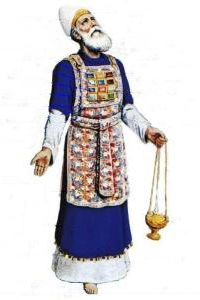
\includegraphics[width=50mm,scale=1.5]{Extras/Melchisedec.jpg}
\vspace{0.4in}  % Create a title for the document and write it in bold font
\LARGE{\textbf{\date}} % Again, do a line break
\linebreak 
% Create a subtitle \large{with Outlines, Statistics, Cross References, and Notes}
\vspace{0.5in}
\begin{flushleft}
\LARGE{Day \#82: Wednesday, 23  March 2022  \\}\vspace{0.25in}
\LARGE{1 Samuel 1-3 Psalm 82 Proverb 23}
\end{flushleft}
\vspace{0.6in}
\bigskip

\normalsize{Xenia, Oh.\\}
\normalsize{created: \today}
\vspace{1.3in}

\end{flushright}
\end{titlepage}

\newpage 
\tableofcontents\hypertarget{TOC}{}
\listoffigures
\listoftables

\hyphenation{A-bim-e-lech bre-thren E-phra-im  Gib-e-o-nites Jer-u-sa-lem through-out Phil-i-stines The-o-phil-us Am-a-le-kites ven-geance Mesh-el-e-mi-ah onan-ism Phar-a-oh thoughts grev-ous-ness Hach-a-liah adul-ter-er Shad-rach}

%%%%%%%%%%%%%%%%% EXTRA COLORS
%%%%%%%%%%%%%%%%% EXTRA COLORS
%%%%%%%%%%%%%%%%% EXTRA COLORS
\definecolor{champagne}{rgb}{0.97,0.91,0.81}
\definecolor{bone}{rgb}{0.89,0.85,0.79}

\definecolor{ForestGreen}{rgb}{0.00,0.29,0.098}
\definecolor{GIVING}{cmyk}{1,0.0,0.72,.1}

\definecolor{MLPE}{cmyk}{1,1,0,.45}
\definecolor{SOCCER}{cmyk}{.77, 0, .42, .49}
\definecolor{PAYBILL}{cmyk}{0,0.83,0.76,0.07}
\definecolor{SERMON}{cmyk}{.14,.9,0,.30} % aka seance \href{http://www.flatuicolorpicker.com/purple-cmyk-color-model/}{seance}
\definecolor{BIBLE}{cmyk}{0,.17,.74,.17}
\definecolor{WORKBLUE}{cmyk}{1, .5, 0, .6}
\definecolor{myOrange}{cmyk}{0, .4, .98, .03}
\definecolor{myTan}{cmyk}{0.0,.07,.17,.10}
\definecolor{myRed}{cmyk}{0,1,1,0}
\definecolor{myWhite}{cmyk}{0,0,0,0}
\definecolor{BLUESoD}{cmyk}{.97,.84,0,.04}
\definecolor{WHITE}{cmyk}{0,0,0,0}
\definecolor{OLDGOLD}{cmyk}{0.05,0.3,1.00,0}
\definecolor{CASTLETON}{cmyk}{1,0,0.31,0.66}
\definecolor{cadmiumgreen}{rgb}{0.0, 0.42, 0.24}
\definecolor{jungle}{rgb}{0.203,0.4882,0.1718}
\definecolor{MYGOLD}{rgb}{1,.84,0}

\definecolor{MYLIGHTGRAY}{rgb}{.85,.85,.85}

\definecolor{codegreen}{rgb}{0,0.6,0}
\definecolor{codegray}{rgb}{0.5,0.5,0.5}
\definecolor{codepurple}{rgb}{0.58,0,0.82}
\definecolor{backcolour}{rgb}{0.95,0.95,0.92}


\mdfdefinestyle{MyFrame}{%
    linecolor=blue,
    outerlinewidth=2pt,
    roundcorner=5pt,
    innertopmargin=\baselineskip,
    innerbottommargin=\baselineskip,
    innerrightmargin=10pt,
    innerleftmargin=10pt,
    backgroundcolor=gray!25!white}


\mdfdefinestyle{MyFrame2}{%
    linecolor=black,
    outerlinewidth=2pt,
    roundcorner=5pt,
    innertopmargin=\baselineskip,
    innerbottommargin=\baselineskip,
    innerrightmargin=10pt,
    innerleftmargin=10pt,
    backgroundcolor=yellow!25!white}


%%%%%
%% for PFTTIS list
%%%%%

%%% And Joseph said unto
\index[PFTTIS]{And Joseph said unto!Genesis!Gen 40:008}
\index[PFTTIS]{And Joseph said unto!Genesis!Gen 40:012}
\index[PFTTIS]{And Joseph said unto!Genesis!Gen 41:025}
\index[PFTTIS]{And Joseph said unto!Genesis!Gen 42:014}
\index[PFTTIS]{And Joseph said unto!Genesis!Gen 42:018}
\index[PFTTIS]{And Joseph said unto!Genesis!Gen 44:015}
\index[PFTTIS]{And Joseph said unto!Genesis!Gen 45:003}
\index[PFTTIS]{And Joseph said unto!Genesis!Gen 45:004}
\index[PFTTIS]{And Joseph said unto!Genesis!Gen 46:031}
\index[PFTTIS]{And Joseph said unto!Genesis!Gen 48:009}
\index[PFTTIS]{And Joseph said unto!Genesis!Gen 48:018}
\index[PFTTIS]{And Joseph said unto!Genesis!Gen 50:019}
\index[PFTTIS]{And Joseph said unto!Genesis!Gen 50:024}


%%% a shadow
\index[PFTTIS]{a shadow!1Chronicles!1Chr 029:15}
\index[PFTTIS]{a shadow!Job!Job 008:09}
\index[PFTTIS]{a shadow!Job!Job 014:02}
\index[PFTTIS]{a shadow!Job!Job 017:07}
\index[PFTTIS]{a shadow!Psalm!Psa 102:011}
\index[PFTTIS]{a shadow!Psalm!Psa 144:004}
\index[PFTTIS]{a shadow!Ecclesiastes!Eccl 006:012}
\index[PFTTIS]{a shadow!Ecclesiastes!Eccl 008:013}
\index[PFTTIS]{a shadow!Isaiah!Isa 04:006}
\index[PFTTIS]{a shadow!Isaiah!Isa 25:004}
\index[PFTTIS]{a shadow!Jonah!Jnh 04:06}
\index[PFTTIS]{a shadow!Colossians!Col 02:017}
\index[PFTTIS]{a shadow!Hebews!Heb 10:001}

%%% blessed is the man
\index[PFTTIS]{blessed is the man!Psalm!Psa 001:001}
\index[PFTTIS]{blessed is the man!Psalm!Psa 032:002}
\index[PFTTIS]{blessed is the man!Psalm!Psa 034:008}
\index[PFTTIS]{blessed is the man!Psalm!Psa 065:004}
\index[PFTTIS]{blessed is the man!Psalm!Psa 084:005}
\index[PFTTIS]{blessed is the man!Psalm!Psa 084:012}
\index[PFTTIS]{blessed is the man!Psalm!Psa 094:012}
\index[PFTTIS]{blessed is the man!Psalm!Psa 112:001}
\index[PFTTIS]{blessed is the man!Proverbs!Pro 008:034}
\index[PFTTIS]{blessed is the man!Isaiah!Isa 056:002}
\index[PFTTIS]{blessed is the man!Jeremiah!Jer 017:007}
\index[PFTTIS]{blessed is the man!Romans!Rom 004:008}
\index[PFTTIS]{blessed is the man!James!Jam 001:012}


%%% carry them
\index[PFTTIS]{carry them!Leviticus!Lev 14:045}
\index[PFTTIS]{carry them!Numbers!Num 11:012}
\index[PFTTIS]{carry them!Joshua!Jsh 04:003}
\index[PFTTIS]{carry them!1Samuel!1Sam 20:040}
\index[PFTTIS]{carry them!1Kings!1Kng 08:046}
\index[PFTTIS]{carry them!2Chronicles!2Chr 06:036}
\index[PFTTIS]{carry them!Ezra!Ezra 05:015}
\index[PFTTIS]{carry them!Isaiah!Isa 40:011}
\index[PFTTIS]{carry them!Isaiah!Isa 41:016}
\index[PFTTIS]{carry them!Isaiah!Isa 57:013}
\index[PFTTIS]{carry them!Jeremiah!Jer 20:004}
\index[PFTTIS]{carry them!Jeremiah!Jer 20:005}
\index[PFTTIS]{carry them!Jeremiah!Jer 43:012}


\index[PFTTIS]{good tidings!2Samuel!2Sam 18:027}
\index[PFTTIS]{good tidings!1Kings!1Ki 01:042}
\index[PFTTIS]{good tidings!2Kings!2Ki 07:009 (2x)}
\index[PFTTIS]{good tidings!Isaiah!Isa 40:009 (2x)}
\index[PFTTIS]{good tidings!Isaiah!Isa 41:007}
\index[PFTTIS]{good tidings!Isaiah!Isa 52:007}
\index[PFTTIS]{good tidings!Isaiah!Isa 61:001}
\index[PFTTIS]{good tidings!Nahum!Nah 01:005}
\index[PFTTIS]{good tidings!Luke!Lk 02:010}
\index[PFTTIS]{good tidings!1Thessalonians!1Thess 03:006}


%%% dead body
\index[PFTTIS]{dead body!Leviticus!Lev 21:011}
\index[PFTTIS]{dead body!Numbers!Num 06:006}
\index[PFTTIS]{dead body!Numbers!Num 09:006}
\index[PFTTIS]{dead body!Numbers!Num 09:007}
\index[PFTTIS]{dead body!Numbers!Num 09:010}
\index[PFTTIS]{dead body!Numbers!Num 09:011}
\index[PFTTIS]{dead body!Numbers!Num 09:013}
\index[PFTTIS]{dead body!Numbers!Num 09:016}
\index[PFTTIS]{dead body!2Kings!2Ki 08:005}
\index[PFTTIS]{dead body!Isaiah!Isa 26:019}
\index[PFTTIS]{dead body!Jeremiah!Jer 26:023}
\index[PFTTIS]{dead body!Jeremiah!Jer 36:030}
\index[PFTTIS]{dead body!Haggai!Hag 02:013}

%%% great sea
\index[PFTTIS]{great sea!Numbers!Num 34:006}
\index[PFTTIS]{great sea!Numbers!Num 34:007}
\index[PFTTIS]{great sea!Joshua!Jos 01:004}
\index[PFTTIS]{great sea!Joshua!Jos 09:001}
\index[PFTTIS]{great sea!Joshua!Jos 15:012}
\index[PFTTIS]{great sea!Joshua!Jos 15:047}
\index[PFTTIS]{great sea!Joshua!Jos 23:004}
\index[PFTTIS]{great sea!Ezekiel!Eze 47:010}
\index[PFTTIS]{great sea!Ezekiel!Eze 47:015}
\index[PFTTIS]{great sea!Ezekiel!Eze 47:019}
\index[PFTTIS]{great sea!Ezekiel!Eze 47:020}
\index[PFTTIS]{great sea!Ezekiel!Eze 48:028}
\index[PFTTIS]{great sea!Daniel!Dan 07:002}


%%% have forsaken me
\index[PFTTIS]{have forsaken me!Judges!Jdg 10:013}
\index[PFTTIS]{have forsaken me!1Samuel!1Sam 08:008}
\index[PFTTIS]{have forsaken me!1Kings!1Ki 11:033}
\index[PFTTIS]{have forsaken me!2Kings!2Ki 22:017}
\index[PFTTIS]{have forsaken me!2Chronicles!2Chr 12:005}
\index[PFTTIS]{have forsaken me!2Chronicles!2Chr 34:025}
\index[PFTTIS]{have forsaken me!Jeremiah!Jer 01:016}
\index[PFTTIS]{have forsaken me!Jeremiah!Jer 02:013}
\index[PFTTIS]{have forsaken me!Jeremiah!Jer 05:007}
\index[PFTTIS]{have forsaken me!Jeremiah!Jer 05:019}
\index[PFTTIS]{have forsaken me!Jeremiah!Jer 16:011 (2x)}
\index[PFTTIS]{have forsaken me!Jeremiah!Jer 19:004}

%%% no king
\index[PFTTIS]{no king!Judges!Jdg 17:06}
\index[PFTTIS]{no king!Judges!Jdg 18:01}
\index[PFTTIS]{no king!Judges!Jdg 19:01}
\index[PFTTIS]{no king!Judges!Jdg 21:25}
\index[PFTTIS]{no king!1Kings!1Ki 22:47}
\index[PFTTIS]{no king!2Kings!2Ki 23:25}
\index[PFTTIS]{no king!Nehemiah!Neh 13:26}
\index[PFTTIS]{no king!Psalms!Psa 033:016}
\index[PFTTIS]{no king!Proverbs!Pro 30:27}
\index[PFTTIS]{no king!Daniel!Dan 02:10}
\index[PFTTIS]{no king!Hosea!Hos 10:03}
\index[PFTTIS]{no king!Micah!Mic 04:09}
\index[PFTTIS]{no king!John!Jhn 19:15}


%%% rebellious house
\index[PFTTIS]{rebellious house!Exodus!Exo 02:005}
\index[PFTTIS]{rebellious house!Exodus!Exo 02:006}
\index[PFTTIS]{rebellious house!Exodus!Exo 02:008}
\index[PFTTIS]{rebellious house!Exodus!Exo 03:009}
\index[PFTTIS]{rebellious house!Exodus!Exo 03:026}
\index[PFTTIS]{rebellious house!Exodus!Exo 03:027}
\index[PFTTIS]{rebellious house!Exodus!Exo 12:002 (2x)}
\index[PFTTIS]{rebellious house!Exodus!Exo 12:003}
\index[PFTTIS]{rebellious house!Exodus!Exo 12:009}
\index[PFTTIS]{rebellious house!Exodus!Exo 12:025}
\index[PFTTIS]{rebellious house!Exodus!Exo 17:012}
\index[PFTTIS]{rebellious house!Exodus!Exo 24:003}

%%% seek him
\index[PFTTIS]{seek him!Deuteronomy!Deu 04:029}\index[PFTTIS]{seek him!1Samuel!1Sam 23:025}
\index[PFTTIS]{seek him!1Chronicles!1Chr 28:009}
\index[PFTTIS]{seek him!2Chronicles!1Chr 15:002}
\index[PFTTIS]{seek him!Ezra!Ezr 08:022}
\index[PFTTIS]{seek him!Psalms!Psa 022:026}
\index[PFTTIS]{seek him!Psalms!Psa 024:006}
\index[PFTTIS]{seek him!Psalms!Psa 119:002}
\index[PFTTIS]{seek him!SoS!SoS 03:002}
\index[PFTTIS]{seek him!SoS!SoS 06:001}
\index[PFTTIS]{seek him!Hosea!Hos 07:010}
\index[PFTTIS]{seek him!Amos!Amo 05:008}
\index[PFTTIS]{seek him!Hebrews!Heb 11:0063}


%%% seek ye
\index[PFTTIS]{seek ye!Isaiah!Isa 34:016}
\index[PFTTIS]{seek ye!Isaiah!Isa 45:019}
\index[PFTTIS]{seek ye!Isaiah!Isa 55:006}
\index[PFTTIS]{seek ye!Amos!Amos 5:004}
\index[PFTTIS]{seek ye!John!John 1:38}
\index[PFTTIS]{seek ye!John!John 18:4}
\index[PFTTIS]{seek ye!John!John 18:7}
\index[PFTTIS]{seek ye!Matthew!Matt 6:33}
\index[PFTTIS]{seek ye!Numbers!Num 16:10}
\index[PFTTIS]{seek ye!Luke!Luke 12:31}
\index[PFTTIS]{seek ye!Luke!Luke 24:5}
\index[PFTTIS]{seek ye!Psalm!Psa 27:8}
\index[PFTTIS]{seek ye!Zephaniah!Zeph 2:3}

%%% the uncircumcised
\index[PFTTIS]{the uncircumcised!Genesis!Gen 17:014}
\index[PFTTIS]{the uncircumcised!Judges!Jdg 14:003}
\index[PFTTIS]{the uncircumcised!Judges!Jdg 15:018}
\index[PFTTIS]{the uncircumcised!2Samuel!2Sam 01:020}
\index[PFTTIS]{the uncircumcised!Isaiah!Isa 02:001}
\index[PFTTIS]{the uncircumcised!Jeremiah!Jer 09:025}
\index[PFTTIS]{the uncircumcised!Ezekiel!Eze 28:010}
\index[PFTTIS]{the uncircumcised!Ezekiel!Eze 31:018}
\index[PFTTIS]{the uncircumcised!Ezekiel!Eze 32:019}
\index[PFTTIS]{the uncircumcised!Ezekiel!Eze 32:027}
\index[PFTTIS]{the uncircumcised!Ezekiel!Eze 32:028}
\index[PFTTIS]{the uncircumcised!Ezekiel!Eze 32:029}
\index[PFTTIS]{the uncircumcised!Ezekiel!Eze 32:032}

%%% worship him
\index[PFTTIS]{worship him!Psalms!Psa 97:007}
\index[PFTTIS]{worship him!Zephaniah!Zeph 02:011}
\index[PFTTIS]{worship him!Matthew!Matt 02:002}
\index[PFTTIS]{worship him!Matthew!Matt 02:008}
\index[PFTTIS]{worship him!John!John 04:023}
\index[PFTTIS]{worship him!John!John 04:024 (2x)} 
\index[PFTTIS]{worship him!Acts!Acts 17:023}
\index[PFTTIS]{worship him!Hebrews!Heb 01:006}
\index[PFTTIS]{worship him!Revelation!Rev 04:010}
\index[PFTTIS]{worship him!Revelation!Rev 13:008}
\index[PFTTIS]{worship him!Revelation!Rev 14:007}
\index[PFTTIS]{worship him!Revelation!Rev 19:010}


%%%%%
%% for PFTTIS list
%%%%%

%%% afflictions
\index[WFTTIS]{afflictions!Psalms!Psa 34:019}
\index[WFTTIS]{afflictions!Psalms!Psa 132:001}
\index[WFTTIS]{afflictions!Acts!Acts 07:010}
\index[WFTTIS]{afflictions!Acts!Acts 20:023}
\index[WFTTIS]{afflictions!2Corinthians!2Cor 06:004}
\index[WFTTIS]{afflictions!Colossians!Col 01:024}
\index[WFTTIS]{afflictions!1Thessalonians!1Thess 03:003}
\index[WFTTIS]{afflictions!2Timothy!2Tim 01:008}
\index[WFTTIS]{afflictions!2Timothy!2Tim 03:011}
\index[WFTTIS]{afflictions!2Timothy!2Tim 04:005}
\index[WFTTIS]{afflictions!Hebrews!Heb 10:032}
\index[WFTTIS]{afflictions!Hebrews!Heb 10:033}
\index[WFTTIS]{afflictions!1Peter!1Pet 05:009}

%%% acsend
\index[WFTTIS]{acsend!Joshua!Jos 06:05}
\index[WFTTIS]{acsend!Psalm!Psa 024:003}
\index[WFTTIS]{acsend!Psalm!Psa 135:007}
\index[WFTTIS]{acsend!Psalm!Psa 139:008}
\index[WFTTIS]{acsend!Isaiah!Isa 14:013}
\index[WFTTIS]{acsend!Isaiah!Isa 14:014}
\index[WFTTIS]{acsend!Jeremiah!Jer 10:013}
\index[WFTTIS]{acsend!Jeremiah!Jer 51:016}
\index[WFTTIS]{acsend!Ezekiel!Eze 38:009}
\index[WFTTIS]{acsend!John!John 06:062}
\index[WFTTIS]{acsend!John!John 20:017}
\index[WFTTIS]{acsend!Romans!Rom 10:006}
\index[WFTTIS]{acsend!Revelation!Rev 17:008}

%%% Assyrian
\index[WFTTIS]{Assyrian!Isaiah!Isa 10:005}
\index[WFTTIS]{Assyrian!Isaiah!Isa 10:024}
\index[WFTTIS]{Assyrian!Isaiah!Isa 14:025}
\index[WFTTIS]{Assyrian!Isaiah!Isa 19:023}
\index[WFTTIS]{Assyrian!Isaiah!Isa 23:013}
\index[WFTTIS]{Assyrian!Isaiah!Isa 30:031}
\index[WFTTIS]{Assyrian!Isaiah!Isa 31:008}
\index[WFTTIS]{Assyrian!Isaiah!Isa 52:004}
\index[WFTTIS]{Assyrian!Ezekiel!Eze 31:003}
\index[WFTTIS]{Assyrian!Hosea!Hos 05:013}
\index[WFTTIS]{Assyrian!Hosea!Hos 11:005}
\index[WFTTIS]{Assyrian!Micah!Hos 05:005}
\index[WFTTIS]{Assyrian!Micah!Hos 05:006}

%%% blot
\index[WFTTIS]{blot!Exodus!Exo 32:032}
\index[WFTTIS]{blot!Exodus!Exo 32:033}
\index[WFTTIS]{blot!Numbers!Num 05:026}
\index[WFTTIS]{blot!Deuteronomy!Deut 09:014}
\index[WFTTIS]{blot!Deuteronomy!Deut 25:019}
\index[WFTTIS]{blot!Deuteronomy!Deut 29:020}
\index[WFTTIS]{blot!2Kings!2Ki 14:027}
\index[WFTTIS]{blot!Job!Job 31:007}
\index[WFTTIS]{blot!Psalms!Psa 51:001}
\index[WFTTIS]{blot!Psalms!Psa 51:009}
\index[WFTTIS]{blot!Proverbs!Pro 09:007}
\index[WFTTIS]{blot!Jeremiah!Jer 18:023}
\index[WFTTIS]{blot!Revelation!Rev 03:005}


%%% chain
\index[WFTTIS]{chain!Genesis!Gen 41:042}
\index[WFTTIS]{chain!1Kings!1Ki 07:017}
\index[WFTTIS]{chain!Psalms!Psa 73:006}
\index[WFTTIS]{chain!SoS!Sos 04:009}
\index[WFTTIS]{chain!Lamentations!Lam 03:007}
\index[WFTTIS]{chain!Ezekiel!Eze 07:023}
\index[WFTTIS]{chain!Ezekiel!Eze 16:011}
\index[WFTTIS]{chain!Daniel!Dan 05:007}
\index[WFTTIS]{chain!Daniel!Dan 05:016}
\index[WFTTIS]{chain!Daniel!Dan 05:029}
\index[WFTTIS]{chain!Acts!Acts 28:020}
\index[WFTTIS]{chain!2Timothy!2Tim 01:016}
\index[WFTTIS]{chain!Revelation!Rev 20:001}


%%% controversy
\index[WFTTIS]{controversy!Deuteronomy!Deu 17:008}
\index[WFTTIS]{controversy!Deuteronomy!Deu 19:017}
\index[WFTTIS]{controversy!Deuteronomy!Deu 21:005}
\index[WFTTIS]{controversy!Deuteronomy!Deu 25:001}
\index[WFTTIS]{controversy!2Samuel!2Sam 15:002}
\index[WFTTIS]{controversy!Isaiah!Isa 34:008}
\index[WFTTIS]{controversy!Jeremiah!Jer 25:031}
\index[WFTTIS]{controversy!Ezekiel!Eze 44:024}
\index[WFTTIS]{controversy!Hosea!Hos 04:001}
\index[WFTTIS]{controversy!Hosea!Hos 12:002}
\index[WFTTIS]{controversy!Micah!Mic 06:002 (2x)}
\index[WFTTIS]{controversy!1Timothy!1Tim 03:016}


%%% Dagon/Dagon's
\index[WFTTIS]{Dagon!Judges!Jdg 16:023}
\index[WFTTIS]{Dagon!1Samuel!1Sam 05:002 (2x)}
\index[WFTTIS]{Dagon!1Samuel!1Sam 05:003 (2x)}
\index[WFTTIS]{Dagon!1Samuel!1Sam 05:004 (3x)}
\index[WFTTIS]{Dagon!1Samuel!1Sam 05:005 (3x)}
\index[WFTTIS]{Dagon!1Samuel!1Sam 05:007}
\index[WFTTIS]{Dagon!1Chronicles!1Chr 10:010}

%%% disobedient
\index[WFTTIS]{disobedient!1Kings!1Ki 13:026}
\index[WFTTIS]{disobedient!Nehemiah!Neh 09:026}
\index[WFTTIS]{disobedient!Luke!Luke 01:017}
\index[WFTTIS]{disobedient!Acts!Acts 26:019}
\index[WFTTIS]{disobedient!Romans!Rom 01:030}
\index[WFTTIS]{disobedient!Romans!Rom 10:021}
\index[WFTTIS]{disobedient!1Timothy!1Tim 01:009}
\index[WFTTIS]{disobedient!2Timothy!2Tim 03:002}
\index[WFTTIS]{disobedient!Titus!Titus 01:016}
\index[WFTTIS]{disobedient!Titus!Titus 03:003}
\index[WFTTIS]{disobedient!1Peter!1Pet 02:007}
\index[WFTTIS]{disobedient!1Peter!1Pet 02:008}
\index[WFTTIS]{disobedient!1Peter!1Pet 03:020}


%%% doubt
\index[WFTTIS]{doubt!Genesis!Gen 37:033}
\index[WFTTIS]{doubt!Deuteronomy!Deu 28:066}
\index[WFTTIS]{doubt!Job!Job 12:002}
\index[WFTTIS]{doubt!Matthew!Matt 14:031}
\index[WFTTIS]{doubt!Matthew!Matt 21:021}
\index[WFTTIS]{doubt!Mark!Mk 11:023}
\index[WFTTIS]{doubt!Luke!Lk 11:020}
\index[WFTTIS]{doubt!John!Jhn 10:024}
\index[WFTTIS]{doubt!Acts!Acts 02:012}
\index[WFTTIS]{doubt!Acts!Acts 28:004}
\index[WFTTIS]{doubt!1Corinthians!1Cor 09:010}
\index[WFTTIS]{doubt!Galatians!Gal 04:020}
\index[WFTTIS]{doubt!1John!1Jhn 02:019}


%%% dungeon
\index[WFTTIS]{dungeon!Genesis!Gen 40:015}
\index[WFTTIS]{dungeon!Genesis!Gen 41:014}
\index[WFTTIS]{dungeon!Exodus!Exo 12:029}
\index[WFTTIS]{dungeon!Jeremiah!Jer 37:016}
\index[WFTTIS]{dungeon!Jeremiah!Jer 38:006 (2x)}
\index[WFTTIS]{dungeon!Jeremiah!Jer 38:007}
\index[WFTTIS]{dungeon!Jeremiah!Jer 38:009}
\index[WFTTIS]{dungeon!Jeremiah!Jer 38:010}
\index[WFTTIS]{dungeon!Jeremiah!Jer 38:011}
\index[WFTTIS]{dungeon!Jeremiah!Jer 38:013}
\index[WFTTIS]{dungeon!Lamentations!Lam 03:053}
\index[WFTTIS]{dungeon!Lamentations!Lam 03:055}


%%% error
\index[WFTTIS]{error!2Samuel!2Sam 06:007}
\index[WFTTIS]{error!Job!Job 19:004}
\index[WFTTIS]{error!Ecclesiastes!Ecc 05:006}
\index[WFTTIS]{error!Ecclesiastes!Ecc 10:005}
\index[WFTTIS]{error!Isaiah!Isa 32:006}
\index[WFTTIS]{error!Daniel!Dan 06:004}
\index[WFTTIS]{error!Matthew!Matt 27:064}
\index[WFTTIS]{error!Romans!Rom 01:027}
\index[WFTTIS]{error!James!Jam 05:020}
\index[WFTTIS]{error!2Peter!2Pet 02:018}
\index[WFTTIS]{error!2Peter!2Pet 03:017}
\index[WFTTIS]{error!1John!1Jn 04:006}
\index[WFTTIS]{error!Jude!Jude 01:011}

%%% fourish
\index[WFTTIS]{fourish!Psalms!Psa 072:007}
\index[WFTTIS]{fourish!Psalms!Psa 072:016}
\index[WFTTIS]{fourish!Psalms!Psa 092:007}
\index[WFTTIS]{fourish!Psalms!Psa 092:012}
\index[WFTTIS]{fourish!Psalms!Psa 092:013}
\index[WFTTIS]{fourish!Psalms!Psa 132:018}
\index[WFTTIS]{fourish!Proverbs!Pro 11:28}
\index[WFTTIS]{fourish!Proverbs!Pro 14:11}
\index[WFTTIS]{fourish!Ecclesiastes!Ecc 12:05}
\index[WFTTIS]{fourish!SongOfSolomon!SOS 07:12}
\index[WFTTIS]{fourish!Isaiah!Isa 17:11}
\index[WFTTIS]{fourish!Isaiah!Isa 66:14}
\index[WFTTIS]{fourish!Ezekiel!Eze 17:24}




%%% giants
\index[WFTTIS]{giants!Genesis!Gen 06:004}
\index[WFTTIS]{giants!Numbers!Num 13:033}
\index[WFTTIS]{giants!Deuteronomy!Deut 02:011}
\index[WFTTIS]{giants!Deuteronomy!Deut 02:021}
\index[WFTTIS]{giants!Deuteronomy!Deut 03:011}
\index[WFTTIS]{giants!Deuteronomy!Deut 03:013}
\index[WFTTIS]{giants!Joshua!Josh 12:004}
\index[WFTTIS]{giants!Joshua!Josh 13:012}
\index[WFTTIS]{giants!Joshua!Josh 15:008}
\index[WFTTIS]{giants!Joshua!Josh 17:015}
\index[WFTTIS]{giants!Joshua!Josh 16:016}

%%% good man
\index[WFTTIS]{good man!2 Samuel!2Sa 18:27}
%(1) Psalms 37:23 [5]
%(1) Psalms 112:5 [2]
%(1) Proverbs 12:2 [2]
%(1) Proverbs 13:22 [2]
%(1) Proverbs 14:14 [14]
%(1) Micah 7:2 [2]
%(1) Matthew 12:35 [2]
%(1) Luke 6:45 [2]
%(1) Luke 23:50 [15]
%(1) John 7:12 [17]
%(1) Acts 11:24 [5]
%(1) Romans 5:7 [14]

%%% Hinnom
\index[WFTTIS]{Hinnom!Joshua!Jsh 15:008}
\index[WFTTIS]{Hinnom!Joshua!Jsh 18:016}
\index[WFTTIS]{Hinnom!2Kings!2Ki 23:010}
\index[WFTTIS]{Hinnom!2Chronicles!2Chr 28:003}
\index[WFTTIS]{Hinnom!2Chronicles!2Chr 33:006}
\index[WFTTIS]{Hinnom!Nehemiah!Neh 11:030}
\index[WFTTIS]{Hinnom!Jeremiah!Jer 07:031}
\index[WFTTIS]{Hinnom!Jeremiah!Jer 07:032}
\index[WFTTIS]{Hinnom!Jeremiah!Jer 19:002}
\index[WFTTIS]{Hinnom!Jeremiah!Jer 19:006}
\index[WFTTIS]{Hinnom!Jeremiah!Jer 32:035}

%%% inclined
\index[WFTTIS]{inclined!Judges!Jdg 09:003}
\index[WFTTIS]{inclined!Psalms!Psa 040:001}
\index[WFTTIS]{inclined!Psalms!Psa 116:002}
\index[WFTTIS]{inclined!Psalms!Psa 119:112}
\index[WFTTIS]{inclined!Proverbs!Pro 05:13}
\index[WFTTIS]{inclined!Jeremiah!Jer 07:24}
\index[WFTTIS]{inclined!Jeremiah!Jer 07:26}
\index[WFTTIS]{inclined!Jeremiah!Jer 11:08}
\index[WFTTIS]{inclined!Jeremiah!Jer 17:23}
\index[WFTTIS]{inclined!Jeremiah!Jer 25:04}
\index[WFTTIS]{inclined!Jeremiah!Jer 34:14}
\index[WFTTIS]{inclined!Jeremiah!Jer 35:15}
\index[WFTTIS]{inclined!Jeremiah!Jer 44:05}


%%% laughed
\index[WFTTIS]{laughed!Genesis!Gen 17:017}
\index[WFTTIS]{laughed!Genesis!Gen 18:012}
\index[WFTTIS]{laughed!Genesis!Gen 18:015}
\index[WFTTIS]{laughed!2Kings!2Ki 19:021}
\index[WFTTIS]{laughed!2Chronicles!2Chr 30:010}
\index[WFTTIS]{laughed!Nehemiah!Neh 02:019}
\index[WFTTIS]{laughed!Job!Job 12:004}
\index[WFTTIS]{laughed!Job!Job 29:024}
\index[WFTTIS]{laughed!Isaiah!Isa 37:022}
\index[WFTTIS]{laughed!Ezekiel!Ezek 23:032}
\index[WFTTIS]{laughed!Matthew!Matt 09:024}
\index[WFTTIS]{laughed!Mark!Mk 05:040}
\index[WFTTIS]{laughed!Luke!Lk 08:053}

%%% liar
\index[WFTTIS]{liar!Job!Job 24:025}
\index[WFTTIS]{liar!Proverbs!Pro 17:004}
\index[WFTTIS]{liar!Proverbs!Pro 19:022}
\index[WFTTIS]{liar!Proverbs!Pro 30:006}
\index[WFTTIS]{liar!Jeremiah!Jer 15:018}
\index[WFTTIS]{liar!John!Jhn 08:044}
\index[WFTTIS]{liar!John!Jhn 08:055}
\index[WFTTIS]{liar!Romans!Rom 03:004}
\index[WFTTIS]{liar!1John!1Jhn 01:010}
\index[WFTTIS]{liar!1John!1Jhn 02:004}
\index[WFTTIS]{liar!1John!1Jhn 02:022}
\index[WFTTIS]{liar!1John!1Jhn 04:020}
\index[WFTTIS]{liar!1John!1Jhn 05:010}

%%% palsy
\index[WFTTIS]{palsy!Matthew!Matt 04:024}
\index[WFTTIS]{palsy!Matthew!Matt 08:006}
\index[WFTTIS]{palsy!Matthew!Matt 09:002}
\index[WFTTIS]{palsy!Matthew!Matt 09:006}
\index[WFTTIS]{palsy!Mark!Mk 02:003}
\index[WFTTIS]{palsy!Mark!Mk 02:004}
\index[WFTTIS]{palsy!Mark!Mk 02:005}
\index[WFTTIS]{palsy!Mark!Mk 02:009}
\index[WFTTIS]{palsy!Mark!Mk 02:010}
\index[WFTTIS]{palsy!Luke!Lk 05:018}
\index[WFTTIS]{palsy!Luke!Lk 05:024}
\index[WFTTIS]{palsy!Acts!Acts 09:033}

%%% Profitable
\index[WFTTIS]{profitable!Job!Job 22:002 (2x)}
\index[WFTTIS]{profitable!Ecclesiastes!Ecc 10:010}
\index[WFTTIS]{profitable!Isaiah!Isa 44:010}
\index[WFTTIS]{profitable!Jeremiah!Jer 13:007}
\index[WFTTIS]{profitable!Matthew!Matt 05:029}
\index[WFTTIS]{profitable!Matthew!Matt 05:030}
\index[WFTTIS]{profitable!Acts!Acts 20:020}
\index[WFTTIS]{profitable!1Timothy!1Tim 04:008}
\index[WFTTIS]{profitable!2Timothy!2Tim 03:016}
\index[WFTTIS]{profitable!2Timothy!2Tim 04:011}
\index[WFTTIS]{profitable!Titus!Titus 03:008}
\index[WFTTIS]{profitable!Philemon!Phlm 01:011}

%%% Rechab
\index[WFTTIS]{Rechab!2Samuel!2Sam 04:002}
\index[WFTTIS]{Rechab!2Samuel!2Sam 04:005}
\index[WFTTIS]{Rechab!2Samuel!2Sam 04:006}
\index[WFTTIS]{Rechab!2Samuel!2Sam 04:009}
\index[WFTTIS]{Rechab!2KIngs!2Ki 10:015}
\index[WFTTIS]{Rechab!2KIngs!2Ki 10:023}
\index[WFTTIS]{Rechab!1Chronicles!1Chr 02:055}
\index[WFTTIS]{Rechab!Nehemiah!Neh 03:014}
\index[WFTTIS]{Rechab!Jeremiah!Jer 35:006}
\index[WFTTIS]{Rechab!Jeremiah!Jer 35:008}
\index[WFTTIS]{Rechab!Jeremiah!Jer 35:014}
\index[WFTTIS]{Rechab!Jeremiah!Jer 35:016}
\index[WFTTIS]{Rechab!Jeremiah!Jer 35:019}

%%% serpents
\index[WFTTIS]{serpents!Exodus!Exo 07:012}
\index[WFTTIS]{serpents!Numbers!Num 21:006}
\index[WFTTIS]{serpents!Numbers!Num 21:007}
\index[WFTTIS]{serpents!Deuteronomy!Deu 08:015}
\index[WFTTIS]{serpents!Deuteronomy!Deu 32:024}
\index[WFTTIS]{serpents!Jeremiah!Jer 08:017}
\index[WFTTIS]{serpents!Matthew!Matt 10:016}
\index[WFTTIS]{serpents!Matthew!Matt 23:033}
\index[WFTTIS]{serpents!Mark!Mk 16:018}
\index[WFTTIS]{serpents!Luke!Lk 10:019}
\index[WFTTIS]{serpents!1Corinthians!1Cor 10:009}
\index[WFTTIS]{serpents!James!Jas 03:007}
\index[WFTTIS]{serpents!Revelation!Rev 09:019}

%%% short
\index[WFTTIS]{short!Numbers!Num 11:023}
\index[WFTTIS]{short!2Kings!2Ki 10:032}
\index[WFTTIS]{short!Job!Job 17:012}
\index[WFTTIS]{short!Job!Job 20:005}
\index[WFTTIS]{short!Psalms!Psa 89:047}
\index[WFTTIS]{short!Romans!Rom 03:023}
\index[WFTTIS]{short!Romans!Rom 09:028  (2x)}
\index[WFTTIS]{short!1Corinthians!1Cor 07:029}
\index[WFTTIS]{short!1Thessalonians!1Thess 02:017}
\index[WFTTIS]{short!Hebrews!Heb 04:001}
\index[WFTTIS]{short!Revelation!Rev 12:012}
\index[WFTTIS]{short!Revelation!Rev 17:010}

%%% smiteth
\index[WFTTIS]{smiteth!Exodus!Exo 21:012}
\index[WFTTIS]{smiteth!Exodus!Exo 21:15}
\index[WFTTIS]{smiteth!Deuteronomy!Dt 25:11}
\index[WFTTIS]{smiteth!Deuteronomy!Dt 27:24}
\index[WFTTIS]{smiteth!Joshua!Jsh 15:16}
\index[WFTTIS]{smiteth!Judges!Jdg 15:16}
\index[WFTTIS]{smiteth!2 Samuel!2Sa 05:08}
\index[WFTTIS]{smiteth!1Chronicles!1Chr 11:06}
\index[WFTTIS]{smiteth!Job!1Chr 26:12}
\index[WFTTIS]{smiteth!Isaiah!Isa 09:13}
\index[WFTTIS]{smiteth!Lamentations!Lam 03:30}
\index[WFTTIS]{smiteth!Ezekiel!Eze 07:09}
\index[WFTTIS]{smiteth!Luke!Lk 06:29}



%%% vanities
\index[WFTTIS]{vanities!Deuteronomy!Deut 21:021}
\index[WFTTIS]{vanities!1Kings!1Ki 16:013}
\index[WFTTIS]{vanities!1Kings!1Ki 16:026}
\index[WFTTIS]{vanities!Psalms!Psa 031:006}
\index[WFTTIS]{vanities!Ecclesiastes!Ecc 01:002 (2x)}
\index[WFTTIS]{vanities!Ecclesiastes!Ecc 05:007}
\index[WFTTIS]{vanities!Ecclesiastes!Ecc 12:008}
\index[WFTTIS]{vanities!Jeremiah!Jer 08:019}
\index[WFTTIS]{vanities!Jeremiah!Jer 10:008}
\index[WFTTIS]{vanities!Jeremiah!Jer 14:022}
\index[WFTTIS]{vanities!Jonah!Jnh 02:008}
\index[WFTTIS]{vanities!Acts!Acts 14:015}



%%%%%
%% for PFTTIS list
%%%%%

%%% worm
\index[WFITV]{worm!Exodus!Exo 16:024}
\index[WFITV]{worm!Job!Job 17:014}
\index[WFITV]{worm!Job!Job 24:029}
\index[WFITV]{worm!Job!Job 25:005 (2x)}
\index[WFITV]{worm!Psalms!Psa 022:006}
\index[WFITV]{worm!Isaiah!Isa 14:011}
\index[WFITV]{worm!Isaiah!Isa 41:014}
\index[WFITV]{worm!Isaiah!Isa 51:008}
\index[WFITV]{worm!Isaiah!Isa 66:024}
\index[WFITV]{worm!Jonah!Jnh 04:007}
\index[WFITV]{worm!Mark!Mk 09:044}
\index[WFITV]{worm!Mark!Mk 09:046}
\index[WFITV]{worm!Mark!Mk 09:048}


%\subsubsection{Title}
%\textbf{Introduction:} Isaiah 46 
%\index[speaker]{Speaker!Isaiah 49 (Title}
%\index[series]{Book (Speaker)!IPassage (Title)}
%\index[date]{2017/07/09!Isaiah 49 (Title)}
%\begin{compactenum}[I.]
%    \item  \textbf{Point} \index[scripture]{Isaiah!IPassage} (IPassage)
%\end{compactenum}




  


%\input{02OT-Exodus/ExodusIntroduction}

\newpage
\begin{figure}
\begin{center}
\includegraphics[scale=0.5, angle=90]{09OT-1Samuel/References/Bible-Project-Samuels}
\caption[1 and 2 Samuel from the Bible Project]{1 and 2 Samuel from the Bible Project}
\label{fig:1 and 2 Samuel from the Bible Project}
\end{center}
\end{figure}

\newpage
\begin{figure}
\begin{center}
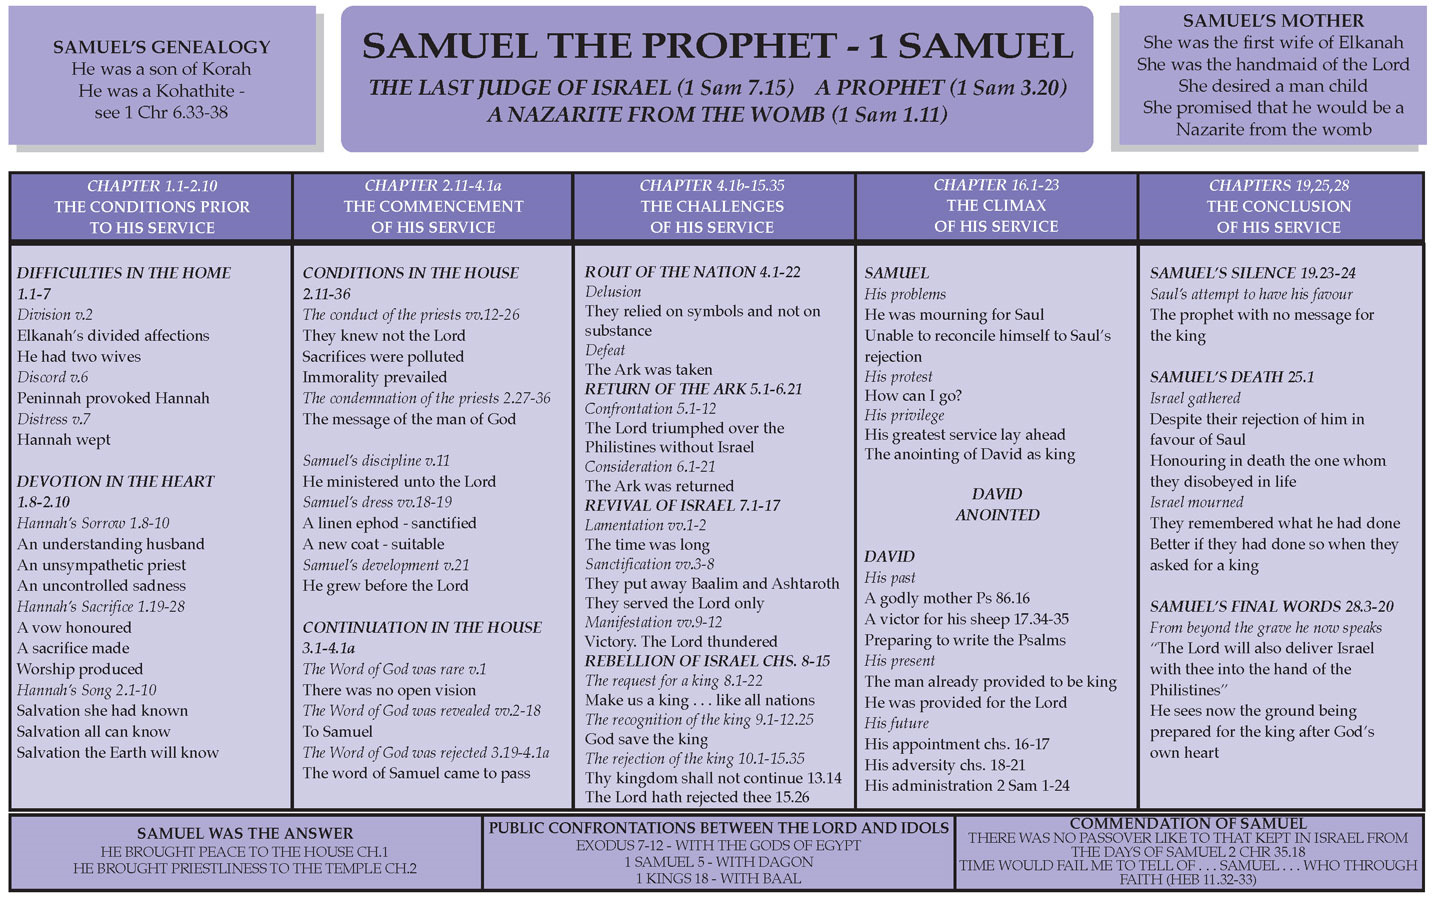
\includegraphics[scale=0.6, angle=90]{09OT-1Samuel/References/Samuel-the-Prophet}
\caption[Samuel the Prophet]{Samuel the Prophet}
\label{fig:Samuel the Prophet}
\end{center}
\end{figure}

\newpage
\begin{figure}
\begin{center}
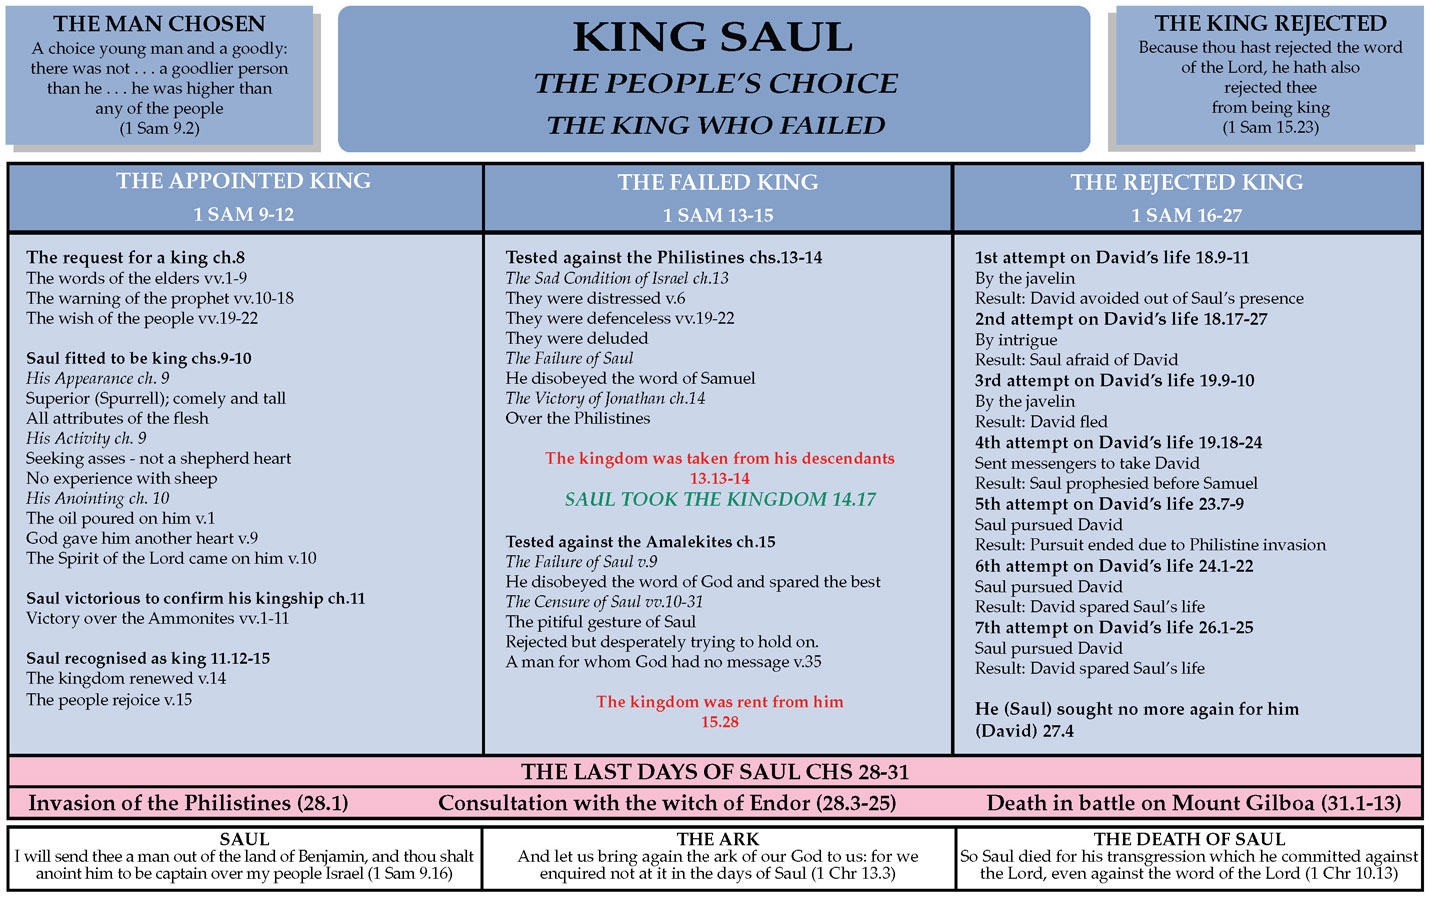
\includegraphics[scale=0.6, angle=90]{09OT-1Samuel/References/King-Saul}
\caption[King Saul]{King Saul}
\label{fig:King Saul}
\end{center}
\end{figure}

\newpage
\begin{figure}
\begin{center}
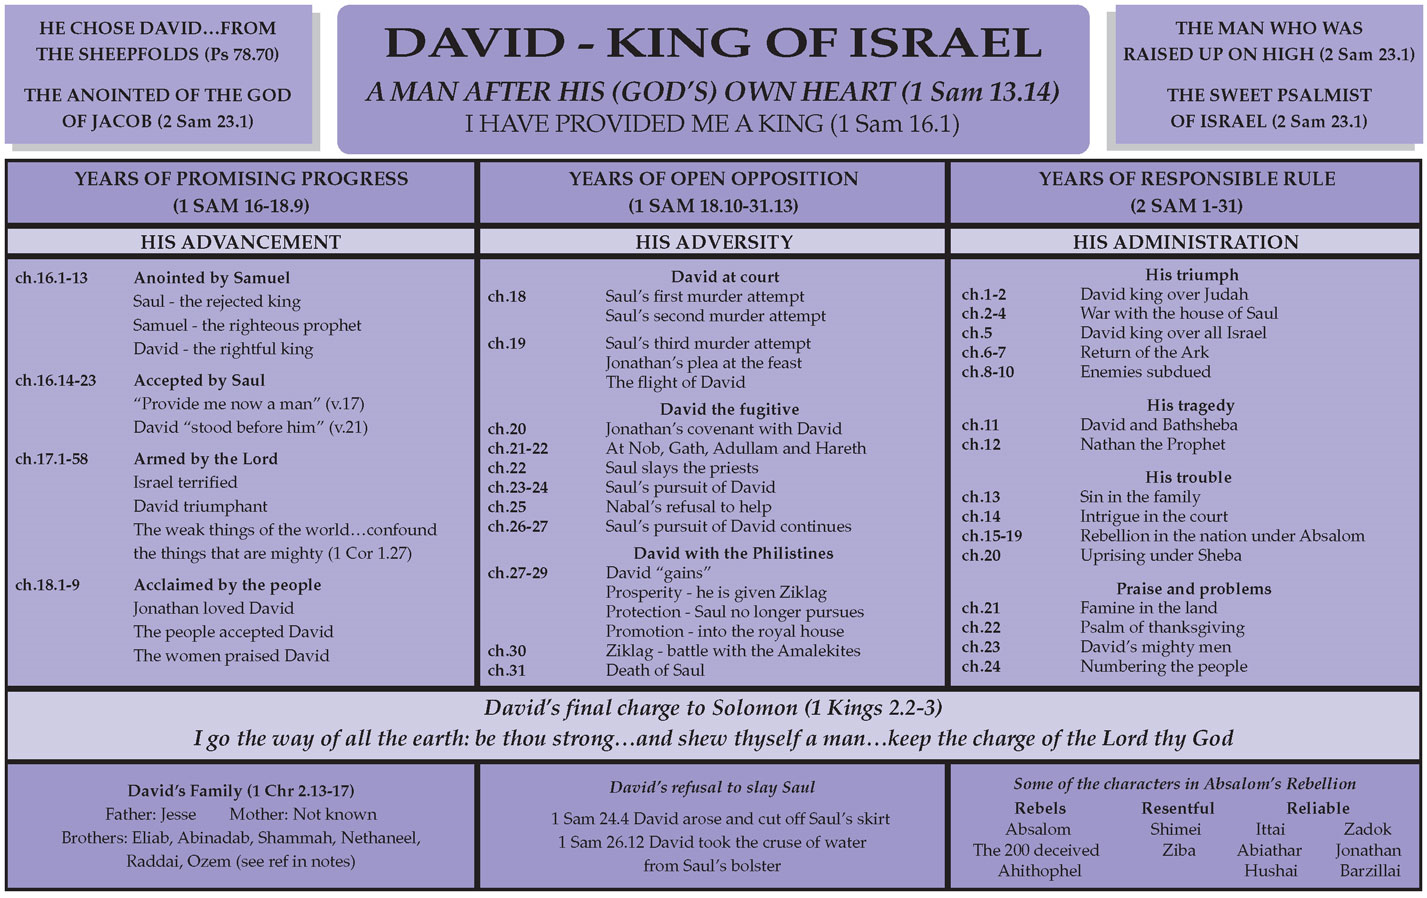
\includegraphics[scale=0.6, angle=90]{09OT-1Samuel/References/David-the-King}
\caption[David the King]{David the King}
\label{fig:David the King}
\end{center}
\end{figure}

\newpage
\begin{figure}
\begin{center}
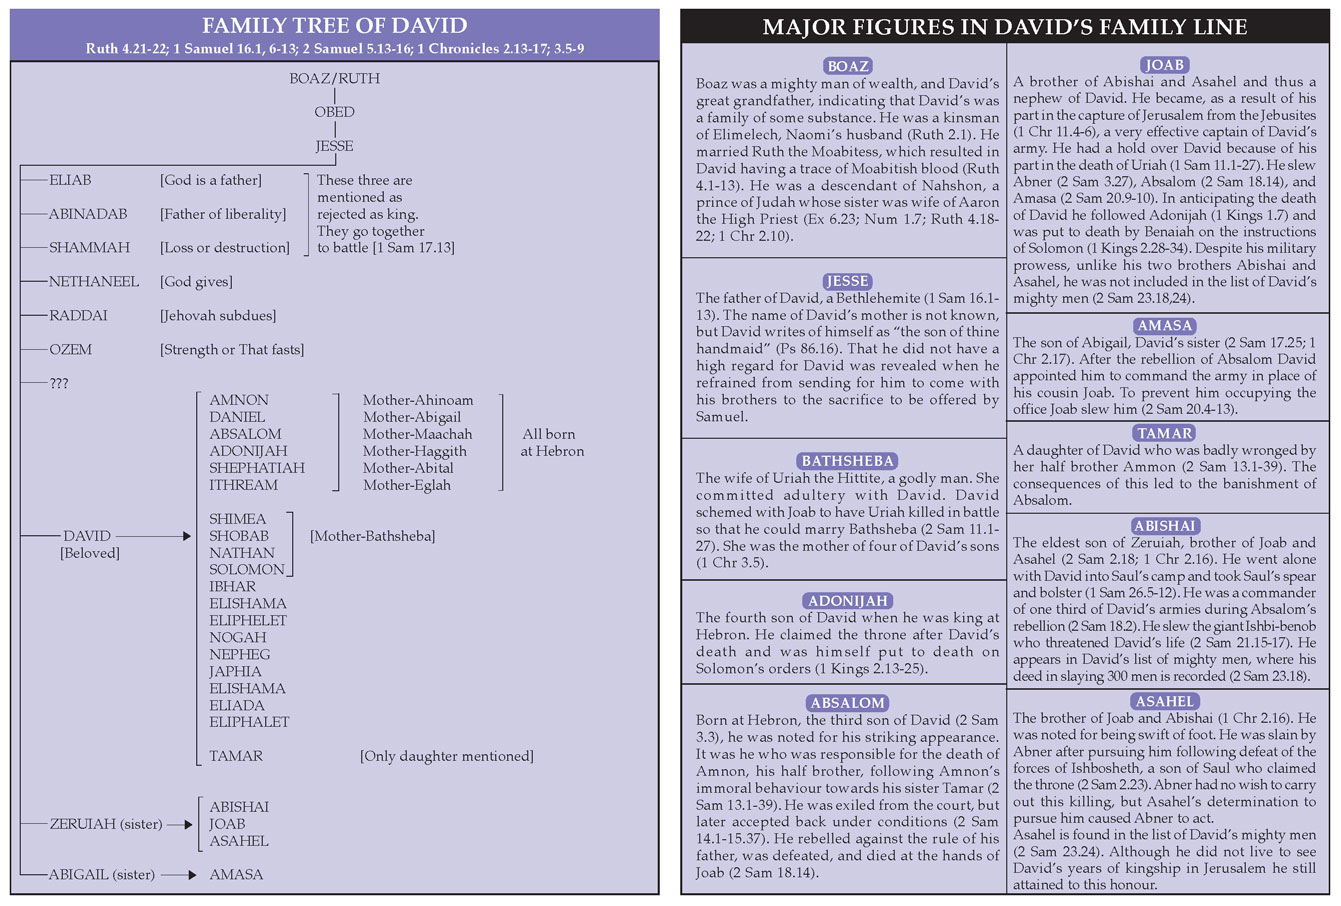
\includegraphics[scale=0.6, angle=90]{09OT-1Samuel/References/Family-of-David}
\caption[Family of David]{Family of David}
\label{fig:Family of David}
\end{center}
\end{figure}



\chapter{1 Samuel 1}



\marginpar{\scriptsize \centering \fcolorbox{bone}{lime}{\textbf{A LENT SON}}\\ (1 Samuel 1:1-28) \begin{compactenum}[I.][8]
    \item A \textbf{Barren Woman}  \index[scripture]{1Samuel!1Sa 01:05}(1Sa 1:5)
    \item \textbf{Bitter \& Weeping}  \index[scripture]{1Samuel!1Sa 01:10}(1Sa 1:10)
    \item \textbf{Belial's Women}  \index[scripture]{1Samuel!1Sa 01:16}(1Sa 1:16)
    \item A \textbf{Baby Awaited}  \index[scripture]{1Samuel!1Sa 01:18}(1Sa 1:18)
    \item The \textbf{Boy Weaned}  \index[scripture]{1Samuel!1Sa 01:23}(1Sa 1:23)
    \item A \textbf{Blessed Woman}  \index[scripture]{1Samuel!1Sa 01:27}(1Sa 1:27)
    \item A \textbf{Boy Worshipping}  \index[scripture]{1Samuel!1Sa 01:28}(1Sa 1:28)
\end{compactenum}}






\footnote{\textcolor[cmyk]{0.99998,1,0,0}{\hyperlink{TOC}{Return to end of Table of Contents.}}}\footnote{\href{https://audiobible.com/bible/1_samuel_1.html}{\textcolor[cmyk]{0.99998,1,0,0}{1 Samuel 1 Audio}}}\textcolor[cmyk]{0.99998,1,0,0}{Now there was a certain man of Ramathaim-zophim, of mount Ephraim, and his name \emph{was} Elkanah, the son of Jeroham, the son of Elihu, the son of Tohu, the son of Zuph, an Ephrathite:}
[2] \textcolor[cmyk]{0.99998,1,0,0}{And he had two wives; the name of the one \emph{was} Hannah, and the name of the other Peninnah: and Peninnah had children, but Hannah had no children.}
[3] \textcolor[cmyk]{0.99998,1,0,0}{And this man went up out of his city yearly to worship and to sacrifice unto the LORD of hosts in Shiloh. And the two sons of Eli, Hophni and Phinehas, the priests of the LORD, \emph{were} there.}\\
\\
\P \textcolor[cmyk]{0.99998,1,0,0}{And when the time was that Elkanah offered, he gave to Peninnah his wife, and to all her sons and her daughters, portions:}
[5] \textcolor[cmyk]{0.99998,1,0,0}{But unto Hannah he gave a worthy portion; for he loved Hannah: but the LORD had \fcolorbox{bone}{lime}{shut up her womb}.}
[6] \textcolor[cmyk]{0.99998,1,0,0}{And her adversary also provoked her sore, for to make her fret, because the LORD had shut up her womb.}
[7] \textcolor[cmyk]{0.99998,1,0,0}{And \emph{as} he did so year by year, when she went up to the house of the LORD, so she provoked her; therefore she wept, and did not eat.}
[8] \textcolor[cmyk]{0.99998,1,0,0}{Then said Elkanah her husband to her, Hannah, why weepest thou? and why eatest thou not? and why is thy heart grieved? \emph{am} not I better to thee than ten sons?}\\
\\
\P \textcolor[cmyk]{0.99998,1,0,0}{So Hannah rose up after they had eaten in Shiloh, and after they had drunk. Now Eli the priest sat upon a seat by a post of the temple of the LORD.}
[10] \textcolor[cmyk]{0.99998,1,0,0}{And she \emph{was} \fcolorbox{bone}{lime}{in bitterness} of soul, and prayed unto the LORD, and wept sore.}
[11] \textcolor[cmyk]{0.99998,1,0,0}{And she vowed a vow, and said, O LORD of hosts, if thou wilt indeed look on the affliction of thine handmaid, and remember me, and not forget thine handmaid, but wilt give unto thine handmaid a man child, then I will give him unto the LORD all the days of his life, and there shall no razor come upon his head.}
[12] \textcolor[cmyk]{0.99998,1,0,0}{And it came to pass, as she continued praying before the LORD, that Eli marked her mouth.}
[13] \textcolor[cmyk]{0.99998,1,0,0}{Now Hannah, she spake in her heart; only her lips moved, but her voice was not heard: therefore Eli thought she had been drunken.}
[14] \textcolor[cmyk]{0.99998,1,0,0}{And Eli said unto her, How long wilt thou be drunken? put away thy wine from thee.}
[15] \textcolor[cmyk]{0.99998,1,0,0}{And Hannah answered and said, No, my lord, I \emph{am} a woman of a sorrowful spirit: I have drunk neither wine nor strong drink, but have poured out my soul before the LORD.}
[16] \textcolor[cmyk]{0.99998,1,0,0}{Count not thine handmaid for a \fcolorbox{bone}{lime}{daughter of Belial}: for out of the abundance of my complaint and grief have I spoken hitherto.}
[17] \textcolor[cmyk]{0.99998,1,0,0}{Then Eli answered and said, Go in peace: and the God of Israel grant \emph{thee} thy petition that thou hast asked of him.}
[18] \textcolor[cmyk]{0.99998,1,0,0}{And she said, Let thine handmaid find grace in thy sight. So the woman went her way, and did eat, and her countenance was no more \emph{sad}.}\\
\\
\P \textcolor[cmyk]{0.99998,1,0,0}{And they rose up in the morning early, and worshipped before the LORD, and returned, and came to their house to Ramah: and Elkanah knew Hannah his wife; and the LORD remembered her.}
[20] \textcolor[cmyk]{0.99998,1,0,0}{Wherefore it came to pass, when the time was come about after Hannah had conceived, that she bare a son, and called his name Samuel, \emph{saying}, Because I have asked him of the LORD.}
[21] \textcolor[cmyk]{0.99998,1,0,0}{And the man Elkanah, and all his house, went up to offer unto the LORD the yearly sacrifice, and his vow.}
[22] \textcolor[cmyk]{0.99998,1,0,0}{But Hannah went not up; for she said unto her husband, \emph{I} \emph{will} \emph{not} \emph{go} \emph{up} until the child be weaned, and \emph{then} I will bring him, that he may appear before the LORD, and there abide for ever.}
[23] \textcolor[cmyk]{0.99998,1,0,0}{And Elkanah her husband said unto her, Do what seemeth thee good; tarry until thou have \fcolorbox{bone}{lime}{weaned} him; only the LORD establish his word. So the woman abode, and gave her son suck until she \fcolorbox{bone}{lime}{weaned} him.}\\
\\
\P \textcolor[cmyk]{0.99998,1,0,0}{And when she had weaned him, she took him up with her, with three bullocks, and one ephah of flour, and a bottle of wine, and brought him unto the house of the LORD in Shiloh: and the child \emph{was} young.}
[25] \textcolor[cmyk]{0.99998,1,0,0}{And they slew a bullock, and brought the child to Eli.}
[26] \textcolor[cmyk]{0.99998,1,0,0}{And she said, Oh my lord, \emph{as} thy soul liveth, my lord, I \emph{am} the woman that stood by thee here, praying unto the LORD.}
[27] \textcolor[cmyk]{0.99998,1,0,0}{For this child I prayed; and the \fcolorbox{bone}{lime}{LORD hath given me} my petition which I asked of him:}
[28] \textcolor[cmyk]{0.99998,1,0,0}{Therefore also I have lent him to the LORD; as long as he liveth he shall be lent to the LORD. And \fcolorbox{bone}{lime}{he worshipped} the LORD there.}
\index[NWIV]{34!1Samuel!1Sa 1:1}\index[AWIP]{Now!1Samuel!1Sa 1:1}\index[AWIP]{there!1Samuel!1Sa 1:1}\index[AWIP]{was!1Samuel!1Sa 1:1}\index[AWIP]{a!1Samuel!1Sa 1:1}\index[AWIP]{certain!1Samuel!1Sa 1:1}\index[AWIP]{man!1Samuel!1Sa 1:1}\index[AWIP]{of!1Samuel!1Sa 1:1}\index[AWIP]{of!1Samuel!1Sa 1:1 (2)}\index[AWIP]{of!1Samuel!1Sa 1:1 (3)}\index[AWIP]{of!1Samuel!1Sa 1:1 (4)}\index[AWIP]{of!1Samuel!1Sa 1:1 (5)}\index[AWIP]{of!1Samuel!1Sa 1:1 (6)}\index[AWIP]{Ramathaim-zophim!1Samuel!1Sa 1:1}\index[AWIP]{mount!1Samuel!1Sa 1:1}\index[AWIP]{Ephraim!1Samuel!1Sa 1:1}\index[AWIP]{and!1Samuel!1Sa 1:1}\index[AWIP]{his!1Samuel!1Sa 1:1}\index[AWIP]{name!1Samuel!1Sa 1:1}\index[AWIP]{\emph{was}!1Samuel!1Sa 1:1}\index[AWIP]{Elkanah!1Samuel!1Sa 1:1}\index[AWIP]{the!1Samuel!1Sa 1:1}\index[AWIP]{the!1Samuel!1Sa 1:1 (2)}\index[AWIP]{the!1Samuel!1Sa 1:1 (3)}\index[AWIP]{the!1Samuel!1Sa 1:1 (4)}\index[AWIP]{son!1Samuel!1Sa 1:1}\index[AWIP]{son!1Samuel!1Sa 1:1 (2)}\index[AWIP]{son!1Samuel!1Sa 1:1 (3)}\index[AWIP]{son!1Samuel!1Sa 1:1 (4)}\index[AWIP]{Jeroham!1Samuel!1Sa 1:1}\index[AWIP]{Elihu!1Samuel!1Sa 1:1}\index[AWIP]{Tohu!1Samuel!1Sa 1:1}\index[AWIP]{Zuph!1Samuel!1Sa 1:1}\index[AWIP]{an!1Samuel!1Sa 1:1}\index[AWIP]{Ephrathite!1Samuel!1Sa 1:1}\index[AWIP]{\emph{was}!1Samuel!1Sa 1:1}

\index[NWIV]{28!1Samuel!1Sa 1:2}\index[AWIP]{And!1Samuel!1Sa 1:2}\index[AWIP]{he!1Samuel!1Sa 1:2}\index[AWIP]{had!1Samuel!1Sa 1:2}\index[AWIP]{had!1Samuel!1Sa 1:2 (2)}\index[AWIP]{had!1Samuel!1Sa 1:2 (3)}\index[AWIP]{two!1Samuel!1Sa 1:2}\index[AWIP]{wives!1Samuel!1Sa 1:2}\index[AWIP]{the!1Samuel!1Sa 1:2}\index[AWIP]{the!1Samuel!1Sa 1:2 (2)}\index[AWIP]{the!1Samuel!1Sa 1:2 (3)}\index[AWIP]{the!1Samuel!1Sa 1:2 (4)}\index[AWIP]{name!1Samuel!1Sa 1:2}\index[AWIP]{name!1Samuel!1Sa 1:2 (2)}\index[AWIP]{of!1Samuel!1Sa 1:2}\index[AWIP]{of!1Samuel!1Sa 1:2 (2)}\index[AWIP]{one!1Samuel!1Sa 1:2}\index[AWIP]{\emph{was}!1Samuel!1Sa 1:2}\index[AWIP]{Hannah!1Samuel!1Sa 1:2}\index[AWIP]{Hannah!1Samuel!1Sa 1:2 (2)}\index[AWIP]{and!1Samuel!1Sa 1:2}\index[AWIP]{and!1Samuel!1Sa 1:2 (2)}\index[AWIP]{other!1Samuel!1Sa 1:2}\index[AWIP]{Peninnah!1Samuel!1Sa 1:2}\index[AWIP]{Peninnah!1Samuel!1Sa 1:2 (2)}\index[AWIP]{children!1Samuel!1Sa 1:2}\index[AWIP]{children!1Samuel!1Sa 1:2 (2)}\index[AWIP]{but!1Samuel!1Sa 1:2}\index[AWIP]{no!1Samuel!1Sa 1:2}\index[AWIP]{\emph{was}!1Samuel!1Sa 1:2}

\index[NWIV]{38!1Samuel!1Sa 1:3}\index[AWIP]{And!1Samuel!1Sa 1:3}\index[AWIP]{And!1Samuel!1Sa 1:3 (2)}\index[AWIP]{this!1Samuel!1Sa 1:3}\index[AWIP]{man!1Samuel!1Sa 1:3}\index[AWIP]{went!1Samuel!1Sa 1:3}\index[AWIP]{up!1Samuel!1Sa 1:3}\index[AWIP]{out!1Samuel!1Sa 1:3}\index[AWIP]{of!1Samuel!1Sa 1:3}\index[AWIP]{of!1Samuel!1Sa 1:3 (2)}\index[AWIP]{of!1Samuel!1Sa 1:3 (3)}\index[AWIP]{of!1Samuel!1Sa 1:3 (4)}\index[AWIP]{his!1Samuel!1Sa 1:3}\index[AWIP]{city!1Samuel!1Sa 1:3}\index[AWIP]{yearly!1Samuel!1Sa 1:3}\index[AWIP]{to!1Samuel!1Sa 1:3}\index[AWIP]{to!1Samuel!1Sa 1:3 (2)}\index[AWIP]{worship!1Samuel!1Sa 1:3}\index[AWIP]{and!1Samuel!1Sa 1:3}\index[AWIP]{and!1Samuel!1Sa 1:3 (2)}\index[AWIP]{sacrifice!1Samuel!1Sa 1:3}\index[AWIP]{unto!1Samuel!1Sa 1:3}\index[AWIP]{the!1Samuel!1Sa 1:3}\index[AWIP]{the!1Samuel!1Sa 1:3 (2)}\index[AWIP]{the!1Samuel!1Sa 1:3 (3)}\index[AWIP]{the!1Samuel!1Sa 1:3 (4)}\index[AWIP]{LORD!1Samuel!1Sa 1:3}\index[AWIP]{LORD!1Samuel!1Sa 1:3 (2)}\index[AWIP]{hosts!1Samuel!1Sa 1:3}\index[AWIP]{in!1Samuel!1Sa 1:3}\index[AWIP]{Shiloh!1Samuel!1Sa 1:3}\index[AWIP]{two!1Samuel!1Sa 1:3}\index[AWIP]{sons!1Samuel!1Sa 1:3}\index[AWIP]{Eli!1Samuel!1Sa 1:3}\index[AWIP]{Hophni!1Samuel!1Sa 1:3}\index[AWIP]{Phinehas!1Samuel!1Sa 1:3}\index[AWIP]{priests!1Samuel!1Sa 1:3}\index[AWIP]{\emph{were}!1Samuel!1Sa 1:3}\index[AWIP]{there!1Samuel!1Sa 1:3}\index[AWIP]{\emph{were}!1Samuel!1Sa 1:3}

\index[NWIV]{23!1Samuel!1Sa 1:4}\index[AWIP]{And!1Samuel!1Sa 1:4}\index[AWIP]{when!1Samuel!1Sa 1:4}\index[AWIP]{the!1Samuel!1Sa 1:4}\index[AWIP]{time!1Samuel!1Sa 1:4}\index[AWIP]{was!1Samuel!1Sa 1:4}\index[AWIP]{that!1Samuel!1Sa 1:4}\index[AWIP]{Elkanah!1Samuel!1Sa 1:4}\index[AWIP]{offered!1Samuel!1Sa 1:4}\index[AWIP]{he!1Samuel!1Sa 1:4}\index[AWIP]{gave!1Samuel!1Sa 1:4}\index[AWIP]{to!1Samuel!1Sa 1:4}\index[AWIP]{to!1Samuel!1Sa 1:4 (2)}\index[AWIP]{Peninnah!1Samuel!1Sa 1:4}\index[AWIP]{his!1Samuel!1Sa 1:4}\index[AWIP]{wife!1Samuel!1Sa 1:4}\index[AWIP]{and!1Samuel!1Sa 1:4}\index[AWIP]{and!1Samuel!1Sa 1:4 (2)}\index[AWIP]{all!1Samuel!1Sa 1:4}\index[AWIP]{her!1Samuel!1Sa 1:4}\index[AWIP]{her!1Samuel!1Sa 1:4 (2)}\index[AWIP]{sons!1Samuel!1Sa 1:4}\index[AWIP]{daughters!1Samuel!1Sa 1:4}\index[AWIP]{portions!1Samuel!1Sa 1:4}

\index[NWIV]{20!1Samuel!1Sa 1:5}\index[AWIP]{But!1Samuel!1Sa 1:5}\index[AWIP]{unto!1Samuel!1Sa 1:5}\index[AWIP]{Hannah!1Samuel!1Sa 1:5}\index[AWIP]{Hannah!1Samuel!1Sa 1:5 (2)}\index[AWIP]{he!1Samuel!1Sa 1:5}\index[AWIP]{he!1Samuel!1Sa 1:5 (2)}\index[AWIP]{gave!1Samuel!1Sa 1:5}\index[AWIP]{a!1Samuel!1Sa 1:5}\index[AWIP]{worthy!1Samuel!1Sa 1:5}\index[AWIP]{portion!1Samuel!1Sa 1:5}\index[AWIP]{for!1Samuel!1Sa 1:5}\index[AWIP]{loved!1Samuel!1Sa 1:5}\index[AWIP]{but!1Samuel!1Sa 1:5}\index[AWIP]{the!1Samuel!1Sa 1:5}\index[AWIP]{LORD!1Samuel!1Sa 1:5}\index[AWIP]{had!1Samuel!1Sa 1:5}\index[AWIP]{shut!1Samuel!1Sa 1:5}\index[AWIP]{up!1Samuel!1Sa 1:5}\index[AWIP]{her!1Samuel!1Sa 1:5}\index[AWIP]{womb!1Samuel!1Sa 1:5}

\index[NWIV]{20!1Samuel!1Sa 1:6}\index[AWIP]{And!1Samuel!1Sa 1:6}\index[AWIP]{her!1Samuel!1Sa 1:6}\index[AWIP]{her!1Samuel!1Sa 1:6 (2)}\index[AWIP]{her!1Samuel!1Sa 1:6 (3)}\index[AWIP]{her!1Samuel!1Sa 1:6 (4)}\index[AWIP]{adversary!1Samuel!1Sa 1:6}\index[AWIP]{also!1Samuel!1Sa 1:6}\index[AWIP]{provoked!1Samuel!1Sa 1:6}\index[AWIP]{sore!1Samuel!1Sa 1:6}\index[AWIP]{for!1Samuel!1Sa 1:6}\index[AWIP]{to!1Samuel!1Sa 1:6}\index[AWIP]{make!1Samuel!1Sa 1:6}\index[AWIP]{fret!1Samuel!1Sa 1:6}\index[AWIP]{because!1Samuel!1Sa 1:6}\index[AWIP]{the!1Samuel!1Sa 1:6}\index[AWIP]{LORD!1Samuel!1Sa 1:6}\index[AWIP]{had!1Samuel!1Sa 1:6}\index[AWIP]{shut!1Samuel!1Sa 1:6}\index[AWIP]{up!1Samuel!1Sa 1:6}\index[AWIP]{womb!1Samuel!1Sa 1:6}

\index[NWIV]{29!1Samuel!1Sa 1:7}\index[AWIP]{And!1Samuel!1Sa 1:7}\index[AWIP]{\emph{as}!1Samuel!1Sa 1:7}\index[AWIP]{he!1Samuel!1Sa 1:7}\index[AWIP]{did!1Samuel!1Sa 1:7}\index[AWIP]{did!1Samuel!1Sa 1:7 (2)}\index[AWIP]{so!1Samuel!1Sa 1:7}\index[AWIP]{so!1Samuel!1Sa 1:7 (2)}\index[AWIP]{year!1Samuel!1Sa 1:7}\index[AWIP]{year!1Samuel!1Sa 1:7 (2)}\index[AWIP]{by!1Samuel!1Sa 1:7}\index[AWIP]{when!1Samuel!1Sa 1:7}\index[AWIP]{she!1Samuel!1Sa 1:7}\index[AWIP]{she!1Samuel!1Sa 1:7 (2)}\index[AWIP]{she!1Samuel!1Sa 1:7 (3)}\index[AWIP]{went!1Samuel!1Sa 1:7}\index[AWIP]{up!1Samuel!1Sa 1:7}\index[AWIP]{to!1Samuel!1Sa 1:7}\index[AWIP]{the!1Samuel!1Sa 1:7}\index[AWIP]{the!1Samuel!1Sa 1:7 (2)}\index[AWIP]{house!1Samuel!1Sa 1:7}\index[AWIP]{of!1Samuel!1Sa 1:7}\index[AWIP]{LORD!1Samuel!1Sa 1:7}\index[AWIP]{provoked!1Samuel!1Sa 1:7}\index[AWIP]{her!1Samuel!1Sa 1:7}\index[AWIP]{therefore!1Samuel!1Sa 1:7}\index[AWIP]{wept!1Samuel!1Sa 1:7}\index[AWIP]{and!1Samuel!1Sa 1:7}\index[AWIP]{not!1Samuel!1Sa 1:7}\index[AWIP]{eat!1Samuel!1Sa 1:7}\index[AWIP]{\emph{as}!1Samuel!1Sa 1:7}

\index[NWIV]{31!1Samuel!1Sa 1:8}\index[AWIP]{Then!1Samuel!1Sa 1:8}\index[AWIP]{said!1Samuel!1Sa 1:8}\index[AWIP]{Elkanah!1Samuel!1Sa 1:8}\index[AWIP]{her!1Samuel!1Sa 1:8}\index[AWIP]{her!1Samuel!1Sa 1:8 (2)}\index[AWIP]{husband!1Samuel!1Sa 1:8}\index[AWIP]{to!1Samuel!1Sa 1:8}\index[AWIP]{to!1Samuel!1Sa 1:8 (2)}\index[AWIP]{Hannah!1Samuel!1Sa 1:8}\index[AWIP]{why!1Samuel!1Sa 1:8}\index[AWIP]{why!1Samuel!1Sa 1:8 (2)}\index[AWIP]{why!1Samuel!1Sa 1:8 (3)}\index[AWIP]{weepest!1Samuel!1Sa 1:8}\index[AWIP]{thou?!1Samuel!1Sa 1:8}\index[AWIP]{and!1Samuel!1Sa 1:8}\index[AWIP]{and!1Samuel!1Sa 1:8 (2)}\index[AWIP]{eatest!1Samuel!1Sa 1:8}\index[AWIP]{thou!1Samuel!1Sa 1:8}\index[AWIP]{not?!1Samuel!1Sa 1:8}\index[AWIP]{is!1Samuel!1Sa 1:8}\index[AWIP]{thy!1Samuel!1Sa 1:8}\index[AWIP]{heart!1Samuel!1Sa 1:8}\index[AWIP]{grieved?!1Samuel!1Sa 1:8}\index[AWIP]{\emph{am}!1Samuel!1Sa 1:8}\index[AWIP]{not!1Samuel!1Sa 1:8}\index[AWIP]{I!1Samuel!1Sa 1:8}\index[AWIP]{better!1Samuel!1Sa 1:8}\index[AWIP]{thee!1Samuel!1Sa 1:8}\index[AWIP]{than!1Samuel!1Sa 1:8}\index[AWIP]{ten!1Samuel!1Sa 1:8}\index[AWIP]{sons?!1Samuel!1Sa 1:8}\index[AWIP]{\emph{am}!1Samuel!1Sa 1:8}

\index[NWIV]{32!1Samuel!1Sa 1:9}\index[AWIP]{So!1Samuel!1Sa 1:9}\index[AWIP]{Hannah!1Samuel!1Sa 1:9}\index[AWIP]{rose!1Samuel!1Sa 1:9}\index[AWIP]{up!1Samuel!1Sa 1:9}\index[AWIP]{after!1Samuel!1Sa 1:9}\index[AWIP]{after!1Samuel!1Sa 1:9 (2)}\index[AWIP]{they!1Samuel!1Sa 1:9}\index[AWIP]{they!1Samuel!1Sa 1:9 (2)}\index[AWIP]{had!1Samuel!1Sa 1:9}\index[AWIP]{had!1Samuel!1Sa 1:9 (2)}\index[AWIP]{eaten!1Samuel!1Sa 1:9}\index[AWIP]{in!1Samuel!1Sa 1:9}\index[AWIP]{Shiloh!1Samuel!1Sa 1:9}\index[AWIP]{and!1Samuel!1Sa 1:9}\index[AWIP]{drunk!1Samuel!1Sa 1:9}\index[AWIP]{Now!1Samuel!1Sa 1:9}\index[AWIP]{Eli!1Samuel!1Sa 1:9}\index[AWIP]{the!1Samuel!1Sa 1:9}\index[AWIP]{the!1Samuel!1Sa 1:9 (2)}\index[AWIP]{the!1Samuel!1Sa 1:9 (3)}\index[AWIP]{priest!1Samuel!1Sa 1:9}\index[AWIP]{sat!1Samuel!1Sa 1:9}\index[AWIP]{upon!1Samuel!1Sa 1:9}\index[AWIP]{a!1Samuel!1Sa 1:9}\index[AWIP]{a!1Samuel!1Sa 1:9 (2)}\index[AWIP]{seat!1Samuel!1Sa 1:9}\index[AWIP]{by!1Samuel!1Sa 1:9}\index[AWIP]{post!1Samuel!1Sa 1:9}\index[AWIP]{of!1Samuel!1Sa 1:9}\index[AWIP]{of!1Samuel!1Sa 1:9 (2)}\index[AWIP]{temple!1Samuel!1Sa 1:9}\index[AWIP]{LORD!1Samuel!1Sa 1:9}

\index[NWIV]{15!1Samuel!1Sa 1:10}\index[AWIP]{And!1Samuel!1Sa 1:10}\index[AWIP]{she!1Samuel!1Sa 1:10}\index[AWIP]{\emph{was}!1Samuel!1Sa 1:10}\index[AWIP]{in!1Samuel!1Sa 1:10}\index[AWIP]{bitterness!1Samuel!1Sa 1:10}\index[AWIP]{of!1Samuel!1Sa 1:10}\index[AWIP]{soul!1Samuel!1Sa 1:10}\index[AWIP]{and!1Samuel!1Sa 1:10}\index[AWIP]{and!1Samuel!1Sa 1:10 (2)}\index[AWIP]{prayed!1Samuel!1Sa 1:10}\index[AWIP]{unto!1Samuel!1Sa 1:10}\index[AWIP]{the!1Samuel!1Sa 1:10}\index[AWIP]{LORD!1Samuel!1Sa 1:10}\index[AWIP]{wept!1Samuel!1Sa 1:10}\index[AWIP]{sore!1Samuel!1Sa 1:10}\index[AWIP]{\emph{was}!1Samuel!1Sa 1:10}

\index[NWIV]{62!1Samuel!1Sa 1:11}\index[AWIP]{And!1Samuel!1Sa 1:11}\index[AWIP]{she!1Samuel!1Sa 1:11}\index[AWIP]{vowed!1Samuel!1Sa 1:11}\index[AWIP]{a!1Samuel!1Sa 1:11}\index[AWIP]{a!1Samuel!1Sa 1:11 (2)}\index[AWIP]{vow!1Samuel!1Sa 1:11}\index[AWIP]{and!1Samuel!1Sa 1:11}\index[AWIP]{and!1Samuel!1Sa 1:11 (2)}\index[AWIP]{and!1Samuel!1Sa 1:11 (3)}\index[AWIP]{and!1Samuel!1Sa 1:11 (4)}\index[AWIP]{said!1Samuel!1Sa 1:11}\index[AWIP]{O!1Samuel!1Sa 1:11}\index[AWIP]{LORD!1Samuel!1Sa 1:11}\index[AWIP]{LORD!1Samuel!1Sa 1:11 (2)}\index[AWIP]{of!1Samuel!1Sa 1:11}\index[AWIP]{of!1Samuel!1Sa 1:11 (2)}\index[AWIP]{of!1Samuel!1Sa 1:11 (3)}\index[AWIP]{hosts!1Samuel!1Sa 1:11}\index[AWIP]{if!1Samuel!1Sa 1:11}\index[AWIP]{thou!1Samuel!1Sa 1:11}\index[AWIP]{wilt!1Samuel!1Sa 1:11}\index[AWIP]{wilt!1Samuel!1Sa 1:11 (2)}\index[AWIP]{indeed!1Samuel!1Sa 1:11}\index[AWIP]{look!1Samuel!1Sa 1:11}\index[AWIP]{on!1Samuel!1Sa 1:11}\index[AWIP]{the!1Samuel!1Sa 1:11}\index[AWIP]{the!1Samuel!1Sa 1:11 (2)}\index[AWIP]{the!1Samuel!1Sa 1:11 (3)}\index[AWIP]{affliction!1Samuel!1Sa 1:11}\index[AWIP]{thine!1Samuel!1Sa 1:11}\index[AWIP]{thine!1Samuel!1Sa 1:11 (2)}\index[AWIP]{thine!1Samuel!1Sa 1:11 (3)}\index[AWIP]{handmaid!1Samuel!1Sa 1:11}\index[AWIP]{handmaid!1Samuel!1Sa 1:11 (2)}\index[AWIP]{handmaid!1Samuel!1Sa 1:11 (3)}\index[AWIP]{remember!1Samuel!1Sa 1:11}\index[AWIP]{me!1Samuel!1Sa 1:11}\index[AWIP]{not!1Samuel!1Sa 1:11}\index[AWIP]{forget!1Samuel!1Sa 1:11}\index[AWIP]{but!1Samuel!1Sa 1:11}\index[AWIP]{give!1Samuel!1Sa 1:11}\index[AWIP]{give!1Samuel!1Sa 1:11 (2)}\index[AWIP]{unto!1Samuel!1Sa 1:11}\index[AWIP]{unto!1Samuel!1Sa 1:11 (2)}\index[AWIP]{man!1Samuel!1Sa 1:11}\index[AWIP]{child!1Samuel!1Sa 1:11}\index[AWIP]{then!1Samuel!1Sa 1:11}\index[AWIP]{I!1Samuel!1Sa 1:11}\index[AWIP]{will!1Samuel!1Sa 1:11}\index[AWIP]{him!1Samuel!1Sa 1:11}\index[AWIP]{all!1Samuel!1Sa 1:11}\index[AWIP]{days!1Samuel!1Sa 1:11}\index[AWIP]{his!1Samuel!1Sa 1:11}\index[AWIP]{his!1Samuel!1Sa 1:11 (2)}\index[AWIP]{life!1Samuel!1Sa 1:11}\index[AWIP]{there!1Samuel!1Sa 1:11}\index[AWIP]{shall!1Samuel!1Sa 1:11}\index[AWIP]{no!1Samuel!1Sa 1:11}\index[AWIP]{razor!1Samuel!1Sa 1:11}\index[AWIP]{come!1Samuel!1Sa 1:11}\index[AWIP]{upon!1Samuel!1Sa 1:11}\index[AWIP]{head!1Samuel!1Sa 1:11}

\index[NWIV]{17!1Samuel!1Sa 1:12}\index[AWIP]{And!1Samuel!1Sa 1:12}\index[AWIP]{it!1Samuel!1Sa 1:12}\index[AWIP]{came!1Samuel!1Sa 1:12}\index[AWIP]{to!1Samuel!1Sa 1:12}\index[AWIP]{pass!1Samuel!1Sa 1:12}\index[AWIP]{as!1Samuel!1Sa 1:12}\index[AWIP]{she!1Samuel!1Sa 1:12}\index[AWIP]{continued!1Samuel!1Sa 1:12}\index[AWIP]{praying!1Samuel!1Sa 1:12}\index[AWIP]{before!1Samuel!1Sa 1:12}\index[AWIP]{the!1Samuel!1Sa 1:12}\index[AWIP]{LORD!1Samuel!1Sa 1:12}\index[AWIP]{that!1Samuel!1Sa 1:12}\index[AWIP]{Eli!1Samuel!1Sa 1:12}\index[AWIP]{marked!1Samuel!1Sa 1:12}\index[AWIP]{her!1Samuel!1Sa 1:12}\index[AWIP]{mouth!1Samuel!1Sa 1:12}

\index[NWIV]{24!1Samuel!1Sa 1:13}\index[AWIP]{Now!1Samuel!1Sa 1:13}\index[AWIP]{Hannah!1Samuel!1Sa 1:13}\index[AWIP]{she!1Samuel!1Sa 1:13}\index[AWIP]{she!1Samuel!1Sa 1:13 (2)}\index[AWIP]{spake!1Samuel!1Sa 1:13}\index[AWIP]{in!1Samuel!1Sa 1:13}\index[AWIP]{her!1Samuel!1Sa 1:13}\index[AWIP]{her!1Samuel!1Sa 1:13 (2)}\index[AWIP]{her!1Samuel!1Sa 1:13 (3)}\index[AWIP]{heart!1Samuel!1Sa 1:13}\index[AWIP]{only!1Samuel!1Sa 1:13}\index[AWIP]{lips!1Samuel!1Sa 1:13}\index[AWIP]{moved!1Samuel!1Sa 1:13}\index[AWIP]{but!1Samuel!1Sa 1:13}\index[AWIP]{voice!1Samuel!1Sa 1:13}\index[AWIP]{was!1Samuel!1Sa 1:13}\index[AWIP]{not!1Samuel!1Sa 1:13}\index[AWIP]{heard!1Samuel!1Sa 1:13}\index[AWIP]{therefore!1Samuel!1Sa 1:13}\index[AWIP]{Eli!1Samuel!1Sa 1:13}\index[AWIP]{thought!1Samuel!1Sa 1:13}\index[AWIP]{had!1Samuel!1Sa 1:13}\index[AWIP]{been!1Samuel!1Sa 1:13}\index[AWIP]{drunken!1Samuel!1Sa 1:13}

\index[NWIV]{17!1Samuel!1Sa 1:14}\index[AWIP]{And!1Samuel!1Sa 1:14}\index[AWIP]{Eli!1Samuel!1Sa 1:14}\index[AWIP]{said!1Samuel!1Sa 1:14}\index[AWIP]{unto!1Samuel!1Sa 1:14}\index[AWIP]{her!1Samuel!1Sa 1:14}\index[AWIP]{How!1Samuel!1Sa 1:14}\index[AWIP]{long!1Samuel!1Sa 1:14}\index[AWIP]{wilt!1Samuel!1Sa 1:14}\index[AWIP]{thou!1Samuel!1Sa 1:14}\index[AWIP]{be!1Samuel!1Sa 1:14}\index[AWIP]{drunken?!1Samuel!1Sa 1:14}\index[AWIP]{put!1Samuel!1Sa 1:14}\index[AWIP]{away!1Samuel!1Sa 1:14}\index[AWIP]{thy!1Samuel!1Sa 1:14}\index[AWIP]{wine!1Samuel!1Sa 1:14}\index[AWIP]{from!1Samuel!1Sa 1:14}\index[AWIP]{thee!1Samuel!1Sa 1:14}

\index[NWIV]{33!1Samuel!1Sa 1:15}\index[AWIP]{And!1Samuel!1Sa 1:15}\index[AWIP]{Hannah!1Samuel!1Sa 1:15}\index[AWIP]{answered!1Samuel!1Sa 1:15}\index[AWIP]{and!1Samuel!1Sa 1:15}\index[AWIP]{said!1Samuel!1Sa 1:15}\index[AWIP]{No!1Samuel!1Sa 1:15}\index[AWIP]{my!1Samuel!1Sa 1:15}\index[AWIP]{my!1Samuel!1Sa 1:15 (2)}\index[AWIP]{lord!1Samuel!1Sa 1:15}\index[AWIP]{I!1Samuel!1Sa 1:15}\index[AWIP]{I!1Samuel!1Sa 1:15 (2)}\index[AWIP]{\emph{am}!1Samuel!1Sa 1:15}\index[AWIP]{a!1Samuel!1Sa 1:15}\index[AWIP]{a!1Samuel!1Sa 1:15 (2)}\index[AWIP]{woman!1Samuel!1Sa 1:15}\index[AWIP]{of!1Samuel!1Sa 1:15}\index[AWIP]{sorrowful!1Samuel!1Sa 1:15}\index[AWIP]{spirit!1Samuel!1Sa 1:15}\index[AWIP]{have!1Samuel!1Sa 1:15}\index[AWIP]{have!1Samuel!1Sa 1:15 (2)}\index[AWIP]{drunk!1Samuel!1Sa 1:15}\index[AWIP]{neither!1Samuel!1Sa 1:15}\index[AWIP]{wine!1Samuel!1Sa 1:15}\index[AWIP]{nor!1Samuel!1Sa 1:15}\index[AWIP]{strong!1Samuel!1Sa 1:15}\index[AWIP]{drink!1Samuel!1Sa 1:15}\index[AWIP]{but!1Samuel!1Sa 1:15}\index[AWIP]{poured!1Samuel!1Sa 1:15}\index[AWIP]{out!1Samuel!1Sa 1:15}\index[AWIP]{soul!1Samuel!1Sa 1:15}\index[AWIP]{before!1Samuel!1Sa 1:15}\index[AWIP]{the!1Samuel!1Sa 1:15}\index[AWIP]{LORD!1Samuel!1Sa 1:15}\index[AWIP]{\emph{am}!1Samuel!1Sa 1:15}

\index[NWIV]{23!1Samuel!1Sa 1:16}\index[AWIP]{Count!1Samuel!1Sa 1:16}\index[AWIP]{not!1Samuel!1Sa 1:16}\index[AWIP]{thine!1Samuel!1Sa 1:16}\index[AWIP]{handmaid!1Samuel!1Sa 1:16}\index[AWIP]{for!1Samuel!1Sa 1:16}\index[AWIP]{for!1Samuel!1Sa 1:16 (2)}\index[AWIP]{a!1Samuel!1Sa 1:16}\index[AWIP]{daughter!1Samuel!1Sa 1:16}\index[AWIP]{of!1Samuel!1Sa 1:16}\index[AWIP]{of!1Samuel!1Sa 1:16 (2)}\index[AWIP]{of!1Samuel!1Sa 1:16 (3)}\index[AWIP]{Belial!1Samuel!1Sa 1:16}\index[AWIP]{out!1Samuel!1Sa 1:16}\index[AWIP]{the!1Samuel!1Sa 1:16}\index[AWIP]{abundance!1Samuel!1Sa 1:16}\index[AWIP]{my!1Samuel!1Sa 1:16}\index[AWIP]{complaint!1Samuel!1Sa 1:16}\index[AWIP]{and!1Samuel!1Sa 1:16}\index[AWIP]{grief!1Samuel!1Sa 1:16}\index[AWIP]{have!1Samuel!1Sa 1:16}\index[AWIP]{I!1Samuel!1Sa 1:16}\index[AWIP]{spoken!1Samuel!1Sa 1:16}\index[AWIP]{hitherto!1Samuel!1Sa 1:16}

\index[NWIV]{23!1Samuel!1Sa 1:17}\index[AWIP]{Then!1Samuel!1Sa 1:17}\index[AWIP]{Eli!1Samuel!1Sa 1:17}\index[AWIP]{answered!1Samuel!1Sa 1:17}\index[AWIP]{and!1Samuel!1Sa 1:17}\index[AWIP]{and!1Samuel!1Sa 1:17 (2)}\index[AWIP]{said!1Samuel!1Sa 1:17}\index[AWIP]{Go!1Samuel!1Sa 1:17}\index[AWIP]{in!1Samuel!1Sa 1:17}\index[AWIP]{peace!1Samuel!1Sa 1:17}\index[AWIP]{the!1Samuel!1Sa 1:17}\index[AWIP]{God!1Samuel!1Sa 1:17}\index[AWIP]{of!1Samuel!1Sa 1:17}\index[AWIP]{of!1Samuel!1Sa 1:17 (2)}\index[AWIP]{Israel!1Samuel!1Sa 1:17}\index[AWIP]{grant!1Samuel!1Sa 1:17}\index[AWIP]{\emph{thee}!1Samuel!1Sa 1:17}\index[AWIP]{thy!1Samuel!1Sa 1:17}\index[AWIP]{petition!1Samuel!1Sa 1:17}\index[AWIP]{that!1Samuel!1Sa 1:17}\index[AWIP]{thou!1Samuel!1Sa 1:17}\index[AWIP]{hast!1Samuel!1Sa 1:17}\index[AWIP]{asked!1Samuel!1Sa 1:17}\index[AWIP]{him!1Samuel!1Sa 1:17}\index[AWIP]{\emph{thee}!1Samuel!1Sa 1:17}

\index[NWIV]{27!1Samuel!1Sa 1:18}\index[AWIP]{And!1Samuel!1Sa 1:18}\index[AWIP]{she!1Samuel!1Sa 1:18}\index[AWIP]{said!1Samuel!1Sa 1:18}\index[AWIP]{Let!1Samuel!1Sa 1:18}\index[AWIP]{thine!1Samuel!1Sa 1:18}\index[AWIP]{handmaid!1Samuel!1Sa 1:18}\index[AWIP]{find!1Samuel!1Sa 1:18}\index[AWIP]{grace!1Samuel!1Sa 1:18}\index[AWIP]{in!1Samuel!1Sa 1:18}\index[AWIP]{thy!1Samuel!1Sa 1:18}\index[AWIP]{sight!1Samuel!1Sa 1:18}\index[AWIP]{So!1Samuel!1Sa 1:18}\index[AWIP]{the!1Samuel!1Sa 1:18}\index[AWIP]{woman!1Samuel!1Sa 1:18}\index[AWIP]{went!1Samuel!1Sa 1:18}\index[AWIP]{her!1Samuel!1Sa 1:18}\index[AWIP]{her!1Samuel!1Sa 1:18 (2)}\index[AWIP]{way!1Samuel!1Sa 1:18}\index[AWIP]{and!1Samuel!1Sa 1:18}\index[AWIP]{and!1Samuel!1Sa 1:18 (2)}\index[AWIP]{did!1Samuel!1Sa 1:18}\index[AWIP]{eat!1Samuel!1Sa 1:18}\index[AWIP]{countenance!1Samuel!1Sa 1:18}\index[AWIP]{was!1Samuel!1Sa 1:18}\index[AWIP]{no!1Samuel!1Sa 1:18}\index[AWIP]{more!1Samuel!1Sa 1:18}\index[AWIP]{\emph{sad}!1Samuel!1Sa 1:18}\index[AWIP]{\emph{sad}!1Samuel!1Sa 1:18}

\index[NWIV]{33!1Samuel!1Sa 1:19}\index[AWIP]{And!1Samuel!1Sa 1:19}\index[AWIP]{they!1Samuel!1Sa 1:19}\index[AWIP]{rose!1Samuel!1Sa 1:19}\index[AWIP]{up!1Samuel!1Sa 1:19}\index[AWIP]{in!1Samuel!1Sa 1:19}\index[AWIP]{the!1Samuel!1Sa 1:19}\index[AWIP]{the!1Samuel!1Sa 1:19 (2)}\index[AWIP]{the!1Samuel!1Sa 1:19 (3)}\index[AWIP]{morning!1Samuel!1Sa 1:19}\index[AWIP]{early!1Samuel!1Sa 1:19}\index[AWIP]{and!1Samuel!1Sa 1:19}\index[AWIP]{and!1Samuel!1Sa 1:19 (2)}\index[AWIP]{and!1Samuel!1Sa 1:19 (3)}\index[AWIP]{and!1Samuel!1Sa 1:19 (4)}\index[AWIP]{and!1Samuel!1Sa 1:19 (5)}\index[AWIP]{worshipped!1Samuel!1Sa 1:19}\index[AWIP]{before!1Samuel!1Sa 1:19}\index[AWIP]{LORD!1Samuel!1Sa 1:19}\index[AWIP]{LORD!1Samuel!1Sa 1:19 (2)}\index[AWIP]{returned!1Samuel!1Sa 1:19}\index[AWIP]{came!1Samuel!1Sa 1:19}\index[AWIP]{to!1Samuel!1Sa 1:19}\index[AWIP]{to!1Samuel!1Sa 1:19 (2)}\index[AWIP]{their!1Samuel!1Sa 1:19}\index[AWIP]{house!1Samuel!1Sa 1:19}\index[AWIP]{Ramah!1Samuel!1Sa 1:19}\index[AWIP]{Elkanah!1Samuel!1Sa 1:19}\index[AWIP]{knew!1Samuel!1Sa 1:19}\index[AWIP]{Hannah!1Samuel!1Sa 1:19}\index[AWIP]{his!1Samuel!1Sa 1:19}\index[AWIP]{wife!1Samuel!1Sa 1:19}\index[AWIP]{remembered!1Samuel!1Sa 1:19}\index[AWIP]{her!1Samuel!1Sa 1:19}

\index[NWIV]{34!1Samuel!1Sa 1:20}\index[AWIP]{Wherefore!1Samuel!1Sa 1:20}\index[AWIP]{it!1Samuel!1Sa 1:20}\index[AWIP]{came!1Samuel!1Sa 1:20}\index[AWIP]{to!1Samuel!1Sa 1:20}\index[AWIP]{pass!1Samuel!1Sa 1:20}\index[AWIP]{when!1Samuel!1Sa 1:20}\index[AWIP]{the!1Samuel!1Sa 1:20}\index[AWIP]{the!1Samuel!1Sa 1:20 (2)}\index[AWIP]{time!1Samuel!1Sa 1:20}\index[AWIP]{was!1Samuel!1Sa 1:20}\index[AWIP]{come!1Samuel!1Sa 1:20}\index[AWIP]{about!1Samuel!1Sa 1:20}\index[AWIP]{after!1Samuel!1Sa 1:20}\index[AWIP]{Hannah!1Samuel!1Sa 1:20}\index[AWIP]{had!1Samuel!1Sa 1:20}\index[AWIP]{conceived!1Samuel!1Sa 1:20}\index[AWIP]{that!1Samuel!1Sa 1:20}\index[AWIP]{she!1Samuel!1Sa 1:20}\index[AWIP]{bare!1Samuel!1Sa 1:20}\index[AWIP]{a!1Samuel!1Sa 1:20}\index[AWIP]{son!1Samuel!1Sa 1:20}\index[AWIP]{and!1Samuel!1Sa 1:20}\index[AWIP]{called!1Samuel!1Sa 1:20}\index[AWIP]{his!1Samuel!1Sa 1:20}\index[AWIP]{name!1Samuel!1Sa 1:20}\index[AWIP]{Samuel!1Samuel!1Sa 1:20}\index[AWIP]{\emph{saying}!1Samuel!1Sa 1:20}\index[AWIP]{Because!1Samuel!1Sa 1:20}\index[AWIP]{I!1Samuel!1Sa 1:20}\index[AWIP]{have!1Samuel!1Sa 1:20}\index[AWIP]{asked!1Samuel!1Sa 1:20}\index[AWIP]{him!1Samuel!1Sa 1:20}\index[AWIP]{of!1Samuel!1Sa 1:20}\index[AWIP]{LORD!1Samuel!1Sa 1:20}\index[AWIP]{\emph{saying}!1Samuel!1Sa 1:20}

\index[NWIV]{21!1Samuel!1Sa 1:21}\index[AWIP]{And!1Samuel!1Sa 1:21}\index[AWIP]{the!1Samuel!1Sa 1:21}\index[AWIP]{the!1Samuel!1Sa 1:21 (2)}\index[AWIP]{the!1Samuel!1Sa 1:21 (3)}\index[AWIP]{man!1Samuel!1Sa 1:21}\index[AWIP]{Elkanah!1Samuel!1Sa 1:21}\index[AWIP]{and!1Samuel!1Sa 1:21}\index[AWIP]{and!1Samuel!1Sa 1:21 (2)}\index[AWIP]{all!1Samuel!1Sa 1:21}\index[AWIP]{his!1Samuel!1Sa 1:21}\index[AWIP]{his!1Samuel!1Sa 1:21 (2)}\index[AWIP]{house!1Samuel!1Sa 1:21}\index[AWIP]{went!1Samuel!1Sa 1:21}\index[AWIP]{up!1Samuel!1Sa 1:21}\index[AWIP]{to!1Samuel!1Sa 1:21}\index[AWIP]{offer!1Samuel!1Sa 1:21}\index[AWIP]{unto!1Samuel!1Sa 1:21}\index[AWIP]{LORD!1Samuel!1Sa 1:21}\index[AWIP]{yearly!1Samuel!1Sa 1:21}\index[AWIP]{sacrifice!1Samuel!1Sa 1:21}\index[AWIP]{vow!1Samuel!1Sa 1:21}

\index[NWIV]{39!1Samuel!1Sa 1:22}\index[AWIP]{But!1Samuel!1Sa 1:22}\index[AWIP]{Hannah!1Samuel!1Sa 1:22}\index[AWIP]{went!1Samuel!1Sa 1:22}\index[AWIP]{not!1Samuel!1Sa 1:22}\index[AWIP]{up!1Samuel!1Sa 1:22}\index[AWIP]{for!1Samuel!1Sa 1:22}\index[AWIP]{for!1Samuel!1Sa 1:22 (2)}\index[AWIP]{she!1Samuel!1Sa 1:22}\index[AWIP]{said!1Samuel!1Sa 1:22}\index[AWIP]{unto!1Samuel!1Sa 1:22}\index[AWIP]{her!1Samuel!1Sa 1:22}\index[AWIP]{husband!1Samuel!1Sa 1:22}\index[AWIP]{\emph{I}!1Samuel!1Sa 1:22}\index[AWIP]{\emph{will}!1Samuel!1Sa 1:22}\index[AWIP]{\emph{not}!1Samuel!1Sa 1:22}\index[AWIP]{\emph{go}!1Samuel!1Sa 1:22}\index[AWIP]{\emph{up}!1Samuel!1Sa 1:22}\index[AWIP]{until!1Samuel!1Sa 1:22}\index[AWIP]{the!1Samuel!1Sa 1:22}\index[AWIP]{the!1Samuel!1Sa 1:22 (2)}\index[AWIP]{child!1Samuel!1Sa 1:22}\index[AWIP]{be!1Samuel!1Sa 1:22}\index[AWIP]{weaned!1Samuel!1Sa 1:22}\index[AWIP]{and!1Samuel!1Sa 1:22}\index[AWIP]{and!1Samuel!1Sa 1:22 (2)}\index[AWIP]{\emph{then}!1Samuel!1Sa 1:22}\index[AWIP]{I!1Samuel!1Sa 1:22}\index[AWIP]{will!1Samuel!1Sa 1:22}\index[AWIP]{bring!1Samuel!1Sa 1:22}\index[AWIP]{him!1Samuel!1Sa 1:22}\index[AWIP]{that!1Samuel!1Sa 1:22}\index[AWIP]{he!1Samuel!1Sa 1:22}\index[AWIP]{may!1Samuel!1Sa 1:22}\index[AWIP]{appear!1Samuel!1Sa 1:22}\index[AWIP]{before!1Samuel!1Sa 1:22}\index[AWIP]{LORD!1Samuel!1Sa 1:22}\index[AWIP]{there!1Samuel!1Sa 1:22}\index[AWIP]{abide!1Samuel!1Sa 1:22}\index[AWIP]{ever!1Samuel!1Sa 1:22}\index[AWIP]{\emph{I}!1Samuel!1Sa 1:22}\index[AWIP]{\emph{will}!1Samuel!1Sa 1:22}\index[AWIP]{\emph{not}!1Samuel!1Sa 1:22}\index[AWIP]{\emph{go}!1Samuel!1Sa 1:22}\index[AWIP]{\emph{up}!1Samuel!1Sa 1:22}\index[AWIP]{\emph{then}!1Samuel!1Sa 1:22}

\index[NWIV]{37!1Samuel!1Sa 1:23}\index[AWIP]{And!1Samuel!1Sa 1:23}\index[AWIP]{Elkanah!1Samuel!1Sa 1:23}\index[AWIP]{her!1Samuel!1Sa 1:23}\index[AWIP]{her!1Samuel!1Sa 1:23 (2)}\index[AWIP]{her!1Samuel!1Sa 1:23 (3)}\index[AWIP]{husband!1Samuel!1Sa 1:23}\index[AWIP]{said!1Samuel!1Sa 1:23}\index[AWIP]{unto!1Samuel!1Sa 1:23}\index[AWIP]{Do!1Samuel!1Sa 1:23}\index[AWIP]{what!1Samuel!1Sa 1:23}\index[AWIP]{seemeth!1Samuel!1Sa 1:23}\index[AWIP]{thee!1Samuel!1Sa 1:23}\index[AWIP]{good!1Samuel!1Sa 1:23}\index[AWIP]{tarry!1Samuel!1Sa 1:23}\index[AWIP]{until!1Samuel!1Sa 1:23}\index[AWIP]{until!1Samuel!1Sa 1:23 (2)}\index[AWIP]{thou!1Samuel!1Sa 1:23}\index[AWIP]{have!1Samuel!1Sa 1:23}\index[AWIP]{weaned!1Samuel!1Sa 1:23}\index[AWIP]{weaned!1Samuel!1Sa 1:23 (2)}\index[AWIP]{him!1Samuel!1Sa 1:23}\index[AWIP]{him!1Samuel!1Sa 1:23 (2)}\index[AWIP]{only!1Samuel!1Sa 1:23}\index[AWIP]{the!1Samuel!1Sa 1:23}\index[AWIP]{the!1Samuel!1Sa 1:23 (2)}\index[AWIP]{LORD!1Samuel!1Sa 1:23}\index[AWIP]{establish!1Samuel!1Sa 1:23}\index[AWIP]{his!1Samuel!1Sa 1:23}\index[AWIP]{word!1Samuel!1Sa 1:23}\index[AWIP]{So!1Samuel!1Sa 1:23}\index[AWIP]{woman!1Samuel!1Sa 1:23}\index[AWIP]{abode!1Samuel!1Sa 1:23}\index[AWIP]{and!1Samuel!1Sa 1:23}\index[AWIP]{gave!1Samuel!1Sa 1:23}\index[AWIP]{son!1Samuel!1Sa 1:23}\index[AWIP]{suck!1Samuel!1Sa 1:23}\index[AWIP]{she!1Samuel!1Sa 1:23}

\index[NWIV]{41!1Samuel!1Sa 1:24}\index[AWIP]{And!1Samuel!1Sa 1:24}\index[AWIP]{when!1Samuel!1Sa 1:24}\index[AWIP]{she!1Samuel!1Sa 1:24}\index[AWIP]{she!1Samuel!1Sa 1:24 (2)}\index[AWIP]{had!1Samuel!1Sa 1:24}\index[AWIP]{weaned!1Samuel!1Sa 1:24}\index[AWIP]{him!1Samuel!1Sa 1:24}\index[AWIP]{him!1Samuel!1Sa 1:24 (2)}\index[AWIP]{him!1Samuel!1Sa 1:24 (3)}\index[AWIP]{took!1Samuel!1Sa 1:24}\index[AWIP]{up!1Samuel!1Sa 1:24}\index[AWIP]{with!1Samuel!1Sa 1:24}\index[AWIP]{with!1Samuel!1Sa 1:24 (2)}\index[AWIP]{her!1Samuel!1Sa 1:24}\index[AWIP]{three!1Samuel!1Sa 1:24}\index[AWIP]{bullocks!1Samuel!1Sa 1:24}\index[AWIP]{and!1Samuel!1Sa 1:24}\index[AWIP]{and!1Samuel!1Sa 1:24 (2)}\index[AWIP]{and!1Samuel!1Sa 1:24 (3)}\index[AWIP]{and!1Samuel!1Sa 1:24 (4)}\index[AWIP]{one!1Samuel!1Sa 1:24}\index[AWIP]{ephah!1Samuel!1Sa 1:24}\index[AWIP]{of!1Samuel!1Sa 1:24}\index[AWIP]{of!1Samuel!1Sa 1:24 (2)}\index[AWIP]{of!1Samuel!1Sa 1:24 (3)}\index[AWIP]{flour!1Samuel!1Sa 1:24}\index[AWIP]{a!1Samuel!1Sa 1:24}\index[AWIP]{bottle!1Samuel!1Sa 1:24}\index[AWIP]{wine!1Samuel!1Sa 1:24}\index[AWIP]{brought!1Samuel!1Sa 1:24}\index[AWIP]{unto!1Samuel!1Sa 1:24}\index[AWIP]{the!1Samuel!1Sa 1:24}\index[AWIP]{the!1Samuel!1Sa 1:24 (2)}\index[AWIP]{the!1Samuel!1Sa 1:24 (3)}\index[AWIP]{house!1Samuel!1Sa 1:24}\index[AWIP]{LORD!1Samuel!1Sa 1:24}\index[AWIP]{in!1Samuel!1Sa 1:24}\index[AWIP]{Shiloh!1Samuel!1Sa 1:24}\index[AWIP]{child!1Samuel!1Sa 1:24}\index[AWIP]{\emph{was}!1Samuel!1Sa 1:24}\index[AWIP]{young!1Samuel!1Sa 1:24}\index[AWIP]{\emph{was}!1Samuel!1Sa 1:24}

\index[NWIV]{11!1Samuel!1Sa 1:25}\index[AWIP]{And!1Samuel!1Sa 1:25}\index[AWIP]{they!1Samuel!1Sa 1:25}\index[AWIP]{slew!1Samuel!1Sa 1:25}\index[AWIP]{a!1Samuel!1Sa 1:25}\index[AWIP]{bullock!1Samuel!1Sa 1:25}\index[AWIP]{and!1Samuel!1Sa 1:25}\index[AWIP]{brought!1Samuel!1Sa 1:25}\index[AWIP]{the!1Samuel!1Sa 1:25}\index[AWIP]{child!1Samuel!1Sa 1:25}\index[AWIP]{to!1Samuel!1Sa 1:25}\index[AWIP]{Eli!1Samuel!1Sa 1:25}

\index[NWIV]{25!1Samuel!1Sa 1:26}\index[AWIP]{And!1Samuel!1Sa 1:26}\index[AWIP]{she!1Samuel!1Sa 1:26}\index[AWIP]{said!1Samuel!1Sa 1:26}\index[AWIP]{Oh!1Samuel!1Sa 1:26}\index[AWIP]{my!1Samuel!1Sa 1:26}\index[AWIP]{my!1Samuel!1Sa 1:26 (2)}\index[AWIP]{lord!1Samuel!1Sa 1:26}\index[AWIP]{lord!1Samuel!1Sa 1:26 (2)}\index[AWIP]{\emph{as}!1Samuel!1Sa 1:26}\index[AWIP]{thy!1Samuel!1Sa 1:26}\index[AWIP]{soul!1Samuel!1Sa 1:26}\index[AWIP]{liveth!1Samuel!1Sa 1:26}\index[AWIP]{I!1Samuel!1Sa 1:26}\index[AWIP]{\emph{am}!1Samuel!1Sa 1:26}\index[AWIP]{the!1Samuel!1Sa 1:26}\index[AWIP]{the!1Samuel!1Sa 1:26 (2)}\index[AWIP]{woman!1Samuel!1Sa 1:26}\index[AWIP]{that!1Samuel!1Sa 1:26}\index[AWIP]{stood!1Samuel!1Sa 1:26}\index[AWIP]{by!1Samuel!1Sa 1:26}\index[AWIP]{thee!1Samuel!1Sa 1:26}\index[AWIP]{here!1Samuel!1Sa 1:26}\index[AWIP]{praying!1Samuel!1Sa 1:26}\index[AWIP]{unto!1Samuel!1Sa 1:26}\index[AWIP]{LORD!1Samuel!1Sa 1:26}\index[AWIP]{\emph{as}!1Samuel!1Sa 1:26}\index[AWIP]{\emph{am}!1Samuel!1Sa 1:26}

\index[NWIV]{18!1Samuel!1Sa 1:27}\index[AWIP]{For!1Samuel!1Sa 1:27}\index[AWIP]{this!1Samuel!1Sa 1:27}\index[AWIP]{child!1Samuel!1Sa 1:27}\index[AWIP]{I!1Samuel!1Sa 1:27}\index[AWIP]{I!1Samuel!1Sa 1:27 (2)}\index[AWIP]{prayed!1Samuel!1Sa 1:27}\index[AWIP]{and!1Samuel!1Sa 1:27}\index[AWIP]{the!1Samuel!1Sa 1:27}\index[AWIP]{LORD!1Samuel!1Sa 1:27}\index[AWIP]{hath!1Samuel!1Sa 1:27}\index[AWIP]{given!1Samuel!1Sa 1:27}\index[AWIP]{me!1Samuel!1Sa 1:27}\index[AWIP]{my!1Samuel!1Sa 1:27}\index[AWIP]{petition!1Samuel!1Sa 1:27}\index[AWIP]{which!1Samuel!1Sa 1:27}\index[AWIP]{asked!1Samuel!1Sa 1:27}\index[AWIP]{of!1Samuel!1Sa 1:27}\index[AWIP]{him!1Samuel!1Sa 1:27}

\index[NWIV]{27!1Samuel!1Sa 1:28}\index[AWIP]{Therefore!1Samuel!1Sa 1:28}\index[AWIP]{also!1Samuel!1Sa 1:28}\index[AWIP]{I!1Samuel!1Sa 1:28}\index[AWIP]{have!1Samuel!1Sa 1:28}\index[AWIP]{lent!1Samuel!1Sa 1:28}\index[AWIP]{lent!1Samuel!1Sa 1:28 (2)}\index[AWIP]{him!1Samuel!1Sa 1:28}\index[AWIP]{to!1Samuel!1Sa 1:28}\index[AWIP]{to!1Samuel!1Sa 1:28 (2)}\index[AWIP]{the!1Samuel!1Sa 1:28}\index[AWIP]{the!1Samuel!1Sa 1:28 (2)}\index[AWIP]{the!1Samuel!1Sa 1:28 (3)}\index[AWIP]{LORD!1Samuel!1Sa 1:28}\index[AWIP]{LORD!1Samuel!1Sa 1:28 (2)}\index[AWIP]{LORD!1Samuel!1Sa 1:28 (3)}\index[AWIP]{as!1Samuel!1Sa 1:28}\index[AWIP]{as!1Samuel!1Sa 1:28 (2)}\index[AWIP]{long!1Samuel!1Sa 1:28}\index[AWIP]{he!1Samuel!1Sa 1:28}\index[AWIP]{he!1Samuel!1Sa 1:28 (2)}\index[AWIP]{he!1Samuel!1Sa 1:28 (3)}\index[AWIP]{liveth!1Samuel!1Sa 1:28}\index[AWIP]{shall!1Samuel!1Sa 1:28}\index[AWIP]{be!1Samuel!1Sa 1:28}\index[AWIP]{And!1Samuel!1Sa 1:28}\index[AWIP]{worshipped!1Samuel!1Sa 1:28}\index[AWIP]{there!1Samuel!1Sa 1:28}


\section{1 Samuel 1 Outlines}

\subsection{My Outlines}

\subsubsection{A Lent Son}
\index[speaker]{Keith Anthony!1 Samuel 01 (A Lent Son)}
\index[series]{1 Samuel (Keith Anthony)!1 Samuel 01 (A Lent Son)}
\index[date]{2019/03/24!1 Samuel 01 (A Lent Son) (Keith Anthony)}

\begin{compactenum}[I.][7]
    \item A \textbf{Barren Woman}  \index[scripture]{1Samuel!1Sa 01:05}(1Sa 1:5)
    \item \textbf{Bitter \& Weeping}  \index[scripture]{1Samuel!1Sa 01:10}(1Sa 1:10)
    \item \textbf{Belial's Women}  \index[scripture]{1Samuel!1Sa 01:16}(1Sa 1:16)
    \item A \textbf{Baby Awaited}  \index[scripture]{1Samuel!1Sa 01:18}(1Sa 1:18)
    \item The \textbf{Boy Weaned}  \index[scripture]{1Samuel!1Sa 01:23}(1Sa 1:23)
    \item A \textbf{Blessed Woman}  \index[scripture]{1Samuel!1Sa 01:27}(1Sa 1:27)
    \item A \textbf{Boy Worshipping}  \index[scripture]{1Samuel!1Sa 01:28}(1Sa 1:28)
\end{compactenum}



\subsection{My Outlines from Others}

\subsubsection{A Son for Hannah}
\index[speaker]{Matt Bernsdorff!1 Samuel 01 (Samuel: A Yearning Heart \& A Baby’s Cry)}
\index[series]{1 Samuel (Matt Bernsdorff)!1 Samuel 01 (Samuel: A Yearning Heart \& A Baby’s Cry)}
\index[date]{unknown!1 Samuel 01 (Samuel: A Yearning Heart \& A Baby’s Cry) (Matt Bernsdorff)}
\textbf{Source: } Highlights Sunday School Curriculum
\begin{compactenum}[I.][7]
    \item The \textbf{Priest}  \index[scripture]{1Samuel!1Sa 01:03}(1Sa 1:3)
    \item A \textbf{Preference}  \index[scripture]{1Samuel!1Sa 01:05}(1Sa 1:5)
    \item The \textbf{Provocation} \index[scripture]{1Samuel!1Sa 01:06} \index[scripture]{1Samuel!1Sa 01:07}  (1Sa 1:6, 7)
    \item The \textbf{Passion} \index[scripture]{1Samuel!1Sa 01:07}(1Sa 1:7)
    \item The \textbf{Petition} \index[scripture]{1Samuel!1Sa 01:11}(1Sa 1:11
    \item The \textbf{Promise} \index[scripture]{1Samuel!1Sa 01:17}(1Sa 1:17)
    \item The \textbf{Presentation} \index[scripture]{1Samuel!1Sa 01:28}(1Sa 1:28)
\end{compactenum}

\subsubsection{God Answers Prayer}
\index[speaker]{Warren Wiersbe!1 Samuel 01 (God Answers Prayer)}
\index[series]{1 Samuel (Warren Wiersbe)!1 Samuel 01 (God Answers Prayer)}
\index[date]{unknown!1 Samuel 01 (God Answers Prayer) (Warren Wiersbe)}
\textbf{Source: }Wiersbe, BE Successful, Commentary on 1 Samuel
\begin{compactenum}[I.][7]
    \item A \textbf{Divided Home}  \index[scripture]{1Samuel!1Sa 01:01--08}(1Sa 1:1--8)
    \item A \textbf{Devout Prayer}  \index[scripture]{1Samuel!1Sa 01:09--19}(1Sa 1:9--18)
    \item A \textbf{Distinguished Son}  \index[scripture]{1Samuel!1Sa 01:19--28}(1Sa 1:19--28)
\end{compactenum}

\section{1 Samuel 1 Comments}


\subsection{1Samuel 1 Repeated Phrases}


%%%%%%%%%%
%%%%%%%%%%
\normalsize
 
\begin{center}
\begin{longtable}{|p{3.0in}|p{0.5in}|}
\caption[1Samuel 1 Repeated Phrases]{1Samuel 1 Repeated Phrases}\label{table:Repeated Phrases 1Samuel 1} \\
\hline \multicolumn{1}{|c|}{\textbf{Phrase}} & \multicolumn{1}{c|}{\textbf{Frequency}} \\ \hline 
\endfirsthead
 
\multicolumn{2}{c}
{{\bfseries \tablename\ \thetable{} -- continued from previous page}} \\  
\hline \multicolumn{1}{|c|}{\textbf{Phrase}} & \multicolumn{1}{c|}{\textbf{Frequency}} \\ \hline 
\endhead
 
\hline \multicolumn{2}{c}{{ }} \\ \hline
\endfoot 
the LORD & 22\\ \hline 
of the & 9\\ \hline 
unto the & 6\\ \hline 
and the & 5\\ \hline 
unto the LORD & 5\\ \hline 
of the LORD & 5\\ \hline 
thine handmaid & 5\\ \hline 
the son & 4\\ \hline 
the son of & 4\\ \hline 
son of & 4\\ \hline 
And she & 4\\ \hline 
before the & 4\\ \hline 
before the LORD & 4\\ \hline 
went up & 3\\ \hline 
in Shiloh & 3\\ \hline 
to the & 3\\ \hline 
her husband & 3\\ \hline 
the LORD and & 3\\ \hline 
LORD and & 3\\ \hline 
and said & 3\\ \hline 
came to & 3\\ \hline 
said unto & 3\\ \hline 
said unto her & 3\\ \hline 
unto her & 3\\ \hline 
my lord & 3\\ \hline 
I have & 3\\ \hline 
she said & 3\\ \hline 
the woman & 3\\ \hline 
the child & 3\\ \hline 
weaned him & 3\\ \hline 
\end{longtable}
\end{center}



%%%%%%%%%%
%%%%%%%%%%



\section{1 Samuel 1 Statistics}

%%%%%%%%%%%%%%%%%%%%%%%%%%%
%%%%% Word Statistics
%%%%%%%%%%%%%%%%%%%%%%%%%%


\normalsize



\subsection{Chapter Word Statistics}


%%%%%%%%%%
%%%%%%%%%%
 
\begin{center}
\begin{longtable}{l|c|c|c|c}
\caption[Stats for FirstSamuel 1]{Stats for FirstSamuel 1} \label{table:Stats for FirstSamuel 1} \\ 
\hline \multicolumn{1}{|c|}{\textbf{Verse(s)}} & \multicolumn{1}{|c|}{\textbf{Count}} & \multicolumn{1}{|c|}{\textbf{Unique}} & \multicolumn{1}{|c|}{\textbf{Italics}} & \multicolumn{1}{|c|}{\textbf{Uniq Italic}}  \\ \hline 
\endfirsthead
 
\multicolumn{5}{c}
{{\bfseries \tablename\ \thetable{} -- continued from previous page}} \\  
\hline \multicolumn{1}{|c|}{\textbf{Verse(s)}} & \multicolumn{1}{|c|}{\textbf{Count}} & \multicolumn{1}{|c|}{\textbf{Unique}} & \multicolumn{1}{|c|}{\textbf{Italics}} & \multicolumn{1}{|c|}{\textbf{Uniq Italic}}  \\ \hline 
\endhead
 
\hline \multicolumn{5}{|r|}{{Continued if needed}} \\ \hline
\endfoot 
1 & 34 & 23 & 1 & 1\\ \hline
2 & 28 & 17 & 1 & 1\\ \hline
3 & 38 & 28 & 1 & 1\\ \hline
4 & 23 & 20 & 0 & 0\\ \hline
5 & 20 & 18 & 0 & 0\\ \hline
6 & 20 & 17 & 0 & 0\\ \hline
7 & 29 & 23 & 1 & 1\\ \hline
8 & 31 & 24 & 1 & 1\\ \hline
9 & 32 & 25 & 0 & 0\\ \hline
10 & 15 & 14 & 1 & 1\\ \hline
11 & 62 & 45 & 0 & 0\\ \hline
12 & 17 & 17 & 0 & 0\\ \hline
13 & 24 & 21 & 0 & 0\\ \hline
14 & 17 & 17 & 0 & 0\\ \hline
15 & 33 & 29 & 1 & 1\\ \hline
16 & 23 & 20 & 0 & 0\\ \hline
17 & 23 & 21 & 1 & 1\\ \hline
18 & 27 & 25 & 1 & 1\\ \hline
19 & 33 & 25 & 0 & 0\\ \hline
20 & 34 & 33 & 1 & 1\\ \hline
21 & 21 & 17 & 0 & 0\\ \hline
22 & 39 & 36 & 6 & 6\\ \hline
23 & 37 & 31 & 0 & 0\\ \hline
24 & 41 & 30 & 1 & 1\\ \hline
25 & 11 & 11 & 0 & 0\\ \hline
26 & 25 & 22 & 2 & 2\\ \hline
27 & 18 & 17 & 0 & 0\\ \hline
28 & 27 & 18 & 0 & 0\\ \hline
\hline \hline
Total & 782 & 270 & 19 & 13



\end{longtable}
\end{center}

%%%%%%%%%%
%%%%%%%%%%
 
\subsection{Words by Frequency}

\begin{center}
\begin{longtable}{l|r}
\caption[Word Frequencies in FirstSamuel 1]{Word Frequencies in FirstSamuel 1} \label{table:WordsIn-FirstSamuel-1} \\ 
\hline \multicolumn{1}{|c|}{\textbf{Word}} & \multicolumn{1}{c|}{\textbf{Frequency}} \\ \hline 
\endfirsthead
 
\multicolumn{2}{c}
{{\bfseries \tablename\ \thetable{} -- continued from previous page}} \\ 
\hline \multicolumn{1}{|c|}{\textbf{Word}} & \multicolumn{1}{c|}{\textbf{Frequency}} \\ \hline 
\endhead
 
\hline \multicolumn{2}{|r|}{{Continued if needed}} \\ \hline
\endfoot
 
\hline \hline
\endlastfoot
the & 51 \\ \hline
and & 40 \\ \hline
of & 30 \\ \hline
LORD & 23 \\ \hline
her & 23 \\ \hline
And & 19 \\ \hline
to & 16 \\ \hline
she & 15 \\ \hline
a & 12 \\ \hline
Hannah & 11 \\ \hline
unto & 11 \\ \hline
I & 11 \\ \hline
him & 11 \\ \hline
his & 10 \\ \hline
had & 10 \\ \hline
he & 9 \\ \hline
up & 9 \\ \hline
said & 9 \\ \hline
in & 8 \\ \hline
Eli & 7 \\ \hline
not & 7 \\ \hline
Elkanah & 6 \\ \hline
son & 6 \\ \hline
that & 6 \\ \hline
for & 6 \\ \hline
thou & 6 \\ \hline
my & 6 \\ \hline
have & 6 \\ \hline
there & 5 \\ \hline
was & 5 \\ \hline
but & 5 \\ \hline
went & 5 \\ \hline
thy & 5 \\ \hline
thine & 5 \\ \hline
handmaid & 5 \\ \hline
child & 5 \\ \hline
man & 4 \\ \hline
name & 4 \\ \hline
\emph{was} & 4 \\ \hline
when & 4 \\ \hline
house & 4 \\ \hline
thee & 4 \\ \hline
they & 4 \\ \hline
before & 4 \\ \hline
woman & 4 \\ \hline
weaned & 4 \\ \hline
Now & 3 \\ \hline
Peninnah & 3 \\ \hline
no & 3 \\ \hline
out & 3 \\ \hline
Shiloh & 3 \\ \hline
sons & 3 \\ \hline
gave & 3 \\ \hline
all & 3 \\ \hline
did & 3 \\ \hline
by & 3 \\ \hline
husband & 3 \\ \hline
why & 3 \\ \hline
\emph{am} & 3 \\ \hline
So & 3 \\ \hline
after & 3 \\ \hline
soul & 3 \\ \hline
wilt & 3 \\ \hline
came & 3 \\ \hline
as & 3 \\ \hline
be & 3 \\ \hline
wine & 3 \\ \hline
lord & 3 \\ \hline
asked & 3 \\ \hline
until & 3 \\ \hline
two & 2 \\ \hline
one & 2 \\ \hline
children & 2 \\ \hline
this & 2 \\ \hline
yearly & 2 \\ \hline
sacrifice & 2 \\ \hline
hosts & 2 \\ \hline
time & 2 \\ \hline
wife & 2 \\ \hline
But & 2 \\ \hline
shut & 2 \\ \hline
womb & 2 \\ \hline
also & 2 \\ \hline
provoked & 2 \\ \hline
sore & 2 \\ \hline
\emph{as} & 2 \\ \hline
so & 2 \\ \hline
year & 2 \\ \hline
therefore & 2 \\ \hline
wept & 2 \\ \hline
eat & 2 \\ \hline
Then & 2 \\ \hline
heart & 2 \\ \hline
rose & 2 \\ \hline
drunk & 2 \\ \hline
upon & 2 \\ \hline
prayed & 2 \\ \hline
vow & 2 \\ \hline
me & 2 \\ \hline
give & 2 \\ \hline
will & 2 \\ \hline
shall & 2 \\ \hline
come & 2 \\ \hline
it & 2 \\ \hline
pass & 2 \\ \hline
praying & 2 \\ \hline
only & 2 \\ \hline
drunken & 2 \\ \hline
long & 2 \\ \hline
answered & 2 \\ \hline
petition & 2 \\ \hline
worshipped & 2 \\ \hline
with & 2 \\ \hline
brought & 2 \\ \hline
liveth & 2 \\ \hline
lent & 2 \\ \hline
certain & 1 \\ \hline
Ramathaim-zophim & 1 \\ \hline
mount & 1 \\ \hline
Ephraim & 1 \\ \hline
Jeroham & 1 \\ \hline
Elihu & 1 \\ \hline
Tohu & 1 \\ \hline
Zuph & 1 \\ \hline
an & 1 \\ \hline
Ephrathite & 1 \\ \hline
wives & 1 \\ \hline
other & 1 \\ \hline
city & 1 \\ \hline
worship & 1 \\ \hline
Hophni & 1 \\ \hline
Phinehas & 1 \\ \hline
priests & 1 \\ \hline
\emph{were} & 1 \\ \hline
offered & 1 \\ \hline
daughters & 1 \\ \hline
portions & 1 \\ \hline
worthy & 1 \\ \hline
portion & 1 \\ \hline
loved & 1 \\ \hline
adversary & 1 \\ \hline
make & 1 \\ \hline
fret & 1 \\ \hline
because & 1 \\ \hline
weepest & 1 \\ \hline
eatest & 1 \\ \hline
is & 1 \\ \hline
grieved & 1 \\ \hline
better & 1 \\ \hline
than & 1 \\ \hline
ten & 1 \\ \hline
eaten & 1 \\ \hline
priest & 1 \\ \hline
sat & 1 \\ \hline
seat & 1 \\ \hline
post & 1 \\ \hline
temple & 1 \\ \hline
bitterness & 1 \\ \hline
vowed & 1 \\ \hline
O & 1 \\ \hline
if & 1 \\ \hline
indeed & 1 \\ \hline
look & 1 \\ \hline
on & 1 \\ \hline
affliction & 1 \\ \hline
remember & 1 \\ \hline
forget & 1 \\ \hline
then & 1 \\ \hline
days & 1 \\ \hline
life & 1 \\ \hline
razor & 1 \\ \hline
head & 1 \\ \hline
continued & 1 \\ \hline
marked & 1 \\ \hline
mouth & 1 \\ \hline
spake & 1 \\ \hline
lips & 1 \\ \hline
moved & 1 \\ \hline
voice & 1 \\ \hline
heard & 1 \\ \hline
thought & 1 \\ \hline
been & 1 \\ \hline
How & 1 \\ \hline
put & 1 \\ \hline
away & 1 \\ \hline
from & 1 \\ \hline
No & 1 \\ \hline
sorrowful & 1 \\ \hline
spirit & 1 \\ \hline
neither & 1 \\ \hline
nor & 1 \\ \hline
strong & 1 \\ \hline
drink & 1 \\ \hline
poured & 1 \\ \hline
Count & 1 \\ \hline
daughter & 1 \\ \hline
Belial & 1 \\ \hline
abundance & 1 \\ \hline
complaint & 1 \\ \hline
grief & 1 \\ \hline
spoken & 1 \\ \hline
hitherto & 1 \\ \hline
Go & 1 \\ \hline
peace & 1 \\ \hline
God & 1 \\ \hline
Israel & 1 \\ \hline
grant & 1 \\ \hline
\emph{thee} & 1 \\ \hline
hast & 1 \\ \hline
Let & 1 \\ \hline
find & 1 \\ \hline
grace & 1 \\ \hline
sight & 1 \\ \hline
way & 1 \\ \hline
countenance & 1 \\ \hline
more & 1 \\ \hline
\emph{sad} & 1 \\ \hline
morning & 1 \\ \hline
early & 1 \\ \hline
returned & 1 \\ \hline
their & 1 \\ \hline
Ramah & 1 \\ \hline
knew & 1 \\ \hline
remembered & 1 \\ \hline
Wherefore & 1 \\ \hline
about & 1 \\ \hline
conceived & 1 \\ \hline
bare & 1 \\ \hline
called & 1 \\ \hline
Samuel & 1 \\ \hline
\emph{saying} & 1 \\ \hline
Because & 1 \\ \hline
offer & 1 \\ \hline
\emph{I} & 1 \\ \hline
\emph{will} & 1 \\ \hline
\emph{not} & 1 \\ \hline
\emph{go} & 1 \\ \hline
\emph{up} & 1 \\ \hline
\emph{then} & 1 \\ \hline
bring & 1 \\ \hline
may & 1 \\ \hline
appear & 1 \\ \hline
abide & 1 \\ \hline
ever & 1 \\ \hline
Do & 1 \\ \hline
what & 1 \\ \hline
seemeth & 1 \\ \hline
good & 1 \\ \hline
tarry & 1 \\ \hline
establish & 1 \\ \hline
word & 1 \\ \hline
abode & 1 \\ \hline
suck & 1 \\ \hline
took & 1 \\ \hline
three & 1 \\ \hline
bullocks & 1 \\ \hline
ephah & 1 \\ \hline
flour & 1 \\ \hline
bottle & 1 \\ \hline
young & 1 \\ \hline
slew & 1 \\ \hline
bullock & 1 \\ \hline
Oh & 1 \\ \hline
stood & 1 \\ \hline
here & 1 \\ \hline
For & 1 \\ \hline
hath & 1 \\ \hline
given & 1 \\ \hline
which & 1 \\ \hline
Therefore & 1 \\ \hline
\end{longtable}
\end{center}



\normalsize



\subsection{Words Alphabetically}

\begin{center}
\begin{longtable}{l|r}
\caption[Word Alphabetically in FirstSamuel 1]{Word Alphabetically in FirstSamuel 1} \label{table:WordsIn-FirstSamuel-1} \\ 
\hline \multicolumn{1}{|c|}{\textbf{Word}} & \multicolumn{1}{c|}{\textbf{Frequency}} \\ \hline 
\endfirsthead
 
\multicolumn{2}{c}
{{\bfseries \tablename\ \thetable{} -- continued from previous page}} \\ 
\hline \multicolumn{1}{|c|}{\textbf{Word}} & \multicolumn{1}{c|}{\textbf{Frequency}} \\ \hline 
\endhead
 
\hline \multicolumn{2}{|r|}{{Continued if needed}} \\ \hline
\endfoot
 
\hline \hline
\endlastfoot
And & 19 \\ \hline
Because & 1 \\ \hline
Belial & 1 \\ \hline
But & 2 \\ \hline
Count & 1 \\ \hline
Do & 1 \\ \hline
Eli & 7 \\ \hline
Elihu & 1 \\ \hline
Elkanah & 6 \\ \hline
Ephraim & 1 \\ \hline
Ephrathite & 1 \\ \hline
For & 1 \\ \hline
Go & 1 \\ \hline
God & 1 \\ \hline
Hannah & 11 \\ \hline
Hophni & 1 \\ \hline
How & 1 \\ \hline
I & 11 \\ \hline
Israel & 1 \\ \hline
Jeroham & 1 \\ \hline
LORD & 23 \\ \hline
Let & 1 \\ \hline
No & 1 \\ \hline
Now & 3 \\ \hline
O & 1 \\ \hline
Oh & 1 \\ \hline
Peninnah & 3 \\ \hline
Phinehas & 1 \\ \hline
Ramah & 1 \\ \hline
Ramathaim-zophim & 1 \\ \hline
Samuel & 1 \\ \hline
Shiloh & 3 \\ \hline
So & 3 \\ \hline
Then & 2 \\ \hline
Therefore & 1 \\ \hline
Tohu & 1 \\ \hline
Wherefore & 1 \\ \hline
Zuph & 1 \\ \hline
\emph{I} & 1 \\ \hline
\emph{am} & 3 \\ \hline
\emph{as} & 2 \\ \hline
\emph{go} & 1 \\ \hline
\emph{not} & 1 \\ \hline
\emph{sad} & 1 \\ \hline
\emph{saying} & 1 \\ \hline
\emph{thee} & 1 \\ \hline
\emph{then} & 1 \\ \hline
\emph{up} & 1 \\ \hline
\emph{was} & 4 \\ \hline
\emph{were} & 1 \\ \hline
\emph{will} & 1 \\ \hline
a & 12 \\ \hline
abide & 1 \\ \hline
abode & 1 \\ \hline
about & 1 \\ \hline
abundance & 1 \\ \hline
adversary & 1 \\ \hline
affliction & 1 \\ \hline
after & 3 \\ \hline
all & 3 \\ \hline
also & 2 \\ \hline
an & 1 \\ \hline
and & 40 \\ \hline
answered & 2 \\ \hline
appear & 1 \\ \hline
as & 3 \\ \hline
asked & 3 \\ \hline
away & 1 \\ \hline
bare & 1 \\ \hline
be & 3 \\ \hline
because & 1 \\ \hline
been & 1 \\ \hline
before & 4 \\ \hline
better & 1 \\ \hline
bitterness & 1 \\ \hline
bottle & 1 \\ \hline
bring & 1 \\ \hline
brought & 2 \\ \hline
bullock & 1 \\ \hline
bullocks & 1 \\ \hline
but & 5 \\ \hline
by & 3 \\ \hline
called & 1 \\ \hline
came & 3 \\ \hline
certain & 1 \\ \hline
child & 5 \\ \hline
children & 2 \\ \hline
city & 1 \\ \hline
come & 2 \\ \hline
complaint & 1 \\ \hline
conceived & 1 \\ \hline
continued & 1 \\ \hline
countenance & 1 \\ \hline
daughter & 1 \\ \hline
daughters & 1 \\ \hline
days & 1 \\ \hline
did & 3 \\ \hline
drink & 1 \\ \hline
drunk & 2 \\ \hline
drunken & 2 \\ \hline
early & 1 \\ \hline
eat & 2 \\ \hline
eaten & 1 \\ \hline
eatest & 1 \\ \hline
ephah & 1 \\ \hline
establish & 1 \\ \hline
ever & 1 \\ \hline
find & 1 \\ \hline
flour & 1 \\ \hline
for & 6 \\ \hline
forget & 1 \\ \hline
fret & 1 \\ \hline
from & 1 \\ \hline
gave & 3 \\ \hline
give & 2 \\ \hline
given & 1 \\ \hline
good & 1 \\ \hline
grace & 1 \\ \hline
grant & 1 \\ \hline
grief & 1 \\ \hline
grieved & 1 \\ \hline
had & 10 \\ \hline
handmaid & 5 \\ \hline
hast & 1 \\ \hline
hath & 1 \\ \hline
have & 6 \\ \hline
he & 9 \\ \hline
head & 1 \\ \hline
heard & 1 \\ \hline
heart & 2 \\ \hline
her & 23 \\ \hline
here & 1 \\ \hline
him & 11 \\ \hline
his & 10 \\ \hline
hitherto & 1 \\ \hline
hosts & 2 \\ \hline
house & 4 \\ \hline
husband & 3 \\ \hline
if & 1 \\ \hline
in & 8 \\ \hline
indeed & 1 \\ \hline
is & 1 \\ \hline
it & 2 \\ \hline
knew & 1 \\ \hline
lent & 2 \\ \hline
life & 1 \\ \hline
lips & 1 \\ \hline
liveth & 2 \\ \hline
long & 2 \\ \hline
look & 1 \\ \hline
lord & 3 \\ \hline
loved & 1 \\ \hline
make & 1 \\ \hline
man & 4 \\ \hline
marked & 1 \\ \hline
may & 1 \\ \hline
me & 2 \\ \hline
more & 1 \\ \hline
morning & 1 \\ \hline
mount & 1 \\ \hline
mouth & 1 \\ \hline
moved & 1 \\ \hline
my & 6 \\ \hline
name & 4 \\ \hline
neither & 1 \\ \hline
no & 3 \\ \hline
nor & 1 \\ \hline
not & 7 \\ \hline
of & 30 \\ \hline
offer & 1 \\ \hline
offered & 1 \\ \hline
on & 1 \\ \hline
one & 2 \\ \hline
only & 2 \\ \hline
other & 1 \\ \hline
out & 3 \\ \hline
pass & 2 \\ \hline
peace & 1 \\ \hline
petition & 2 \\ \hline
portion & 1 \\ \hline
portions & 1 \\ \hline
post & 1 \\ \hline
poured & 1 \\ \hline
prayed & 2 \\ \hline
praying & 2 \\ \hline
priest & 1 \\ \hline
priests & 1 \\ \hline
provoked & 2 \\ \hline
put & 1 \\ \hline
razor & 1 \\ \hline
remember & 1 \\ \hline
remembered & 1 \\ \hline
returned & 1 \\ \hline
rose & 2 \\ \hline
sacrifice & 2 \\ \hline
said & 9 \\ \hline
sat & 1 \\ \hline
seat & 1 \\ \hline
seemeth & 1 \\ \hline
shall & 2 \\ \hline
she & 15 \\ \hline
shut & 2 \\ \hline
sight & 1 \\ \hline
slew & 1 \\ \hline
so & 2 \\ \hline
son & 6 \\ \hline
sons & 3 \\ \hline
sore & 2 \\ \hline
sorrowful & 1 \\ \hline
soul & 3 \\ \hline
spake & 1 \\ \hline
spirit & 1 \\ \hline
spoken & 1 \\ \hline
stood & 1 \\ \hline
strong & 1 \\ \hline
suck & 1 \\ \hline
tarry & 1 \\ \hline
temple & 1 \\ \hline
ten & 1 \\ \hline
than & 1 \\ \hline
that & 6 \\ \hline
the & 51 \\ \hline
thee & 4 \\ \hline
their & 1 \\ \hline
then & 1 \\ \hline
there & 5 \\ \hline
therefore & 2 \\ \hline
they & 4 \\ \hline
thine & 5 \\ \hline
this & 2 \\ \hline
thou & 6 \\ \hline
thought & 1 \\ \hline
three & 1 \\ \hline
thy & 5 \\ \hline
time & 2 \\ \hline
to & 16 \\ \hline
took & 1 \\ \hline
two & 2 \\ \hline
until & 3 \\ \hline
unto & 11 \\ \hline
up & 9 \\ \hline
upon & 2 \\ \hline
voice & 1 \\ \hline
vow & 2 \\ \hline
vowed & 1 \\ \hline
was & 5 \\ \hline
way & 1 \\ \hline
weaned & 4 \\ \hline
weepest & 1 \\ \hline
went & 5 \\ \hline
wept & 2 \\ \hline
what & 1 \\ \hline
when & 4 \\ \hline
which & 1 \\ \hline
why & 3 \\ \hline
wife & 2 \\ \hline
will & 2 \\ \hline
wilt & 3 \\ \hline
wine & 3 \\ \hline
with & 2 \\ \hline
wives & 1 \\ \hline
woman & 4 \\ \hline
womb & 2 \\ \hline
word & 1 \\ \hline
worship & 1 \\ \hline
worshipped & 2 \\ \hline
worthy & 1 \\ \hline
year & 2 \\ \hline
yearly & 2 \\ \hline
young & 1 \\ \hline
\end{longtable}
\end{center}



\normalsize



\subsection{Word Lengths in Chapter}
\normalsize
\begin{longtable}{l|p{3.75in}}
\caption[Words by Length in FirstSamuel 1]{Words by Length in FirstSamuel 1} \label{table:WordsIn-FirstSamuel-1} \\ 
\hline \multicolumn{1}{|c|}{\textbf{Length}} & \multicolumn{1}{c|}{\textbf{Words}} \\ \hline 
\endfirsthead
 
\multicolumn{2}{c}
{{\bfseries \tablename\ \thetable{} -- continued from previous page}} \\ 
\hline \multicolumn{1}{|c|}{\textbf{Length}} & \multicolumn{1}{c|}{\textbf{Words}} \\ \hline 
\endhead
 
\hline \multicolumn{2}{|r|}{{Continued if needed}} \\ \hline
\endfoot
 
\hline \hline
\endlastfoot
1 & a, I, O, \emph{I} \\ \hline
2 & of, an, he, no, up, to, in, \emph{as}, so, by, is, \emph{am}, So, if, on, me, it, as, be, No, my, Go, \emph{go}, \emph{up}, Do, Oh \\ \hline
3 & Now, was, man, and, his, \emph{was}, the, son, And, had, two, one, but, out, Eli, all, her, But, for, did, she, not, eat, why, thy, ten, sat, vow, him, How, put, nor, God, Let, way, \emph{sad}, \emph{not}, may, For \\ \hline
4 & name, Tohu, Zuph, this, went, city, unto, LORD, sons, \emph{were}, when, time, that, gave, wife, shut, womb, also, sore, make, fret, year, wept, Then, said, thou, thee, than, rose, they, upon, seat, post, soul, wilt, look, give, then, will, days, life, come, head, came, pass, only, lips, been, long, away, wine, from, lord, have, \emph{thee}, hast, find, more, knew, bare, \emph{will}, \emph{then}, ever, what, good, word, suck, took, with, slew, here, hath, lent \\ \hline
5 & there, mount, Elihu, wives, other, hosts, loved, house, heart, after, eaten, drunk, vowed, thine, child, shall, razor, mouth, spake, moved, voice, heard, woman, drink, Count, grief, peace, grant, asked, grace, sight, early, their, Ramah, about, offer, until, bring, abide, tarry, abode, three, ephah, flour, young, stood, given, which \\ \hline
6 & Hannah, yearly, Shiloh, Hophni, worthy, eatest, better, priest, temple, prayed, indeed, forget, before, marked, spirit, strong, poured, Belial, spoken, Israel, called, Samuel, \emph{saying}, weaned, appear, bottle, liveth \\ \hline
7 & certain, Ephraim, Elkanah, Jeroham, worship, priests, offered, portion, because, husband, weepest, grieved, praying, thought, drunken, neither, morning, Because, seemeth, brought, bullock \\ \hline
8 & Peninnah, children, Phinehas, portions, provoked, handmaid, remember, answered, daughter, hitherto, petition, returned, bullocks \\ \hline
9 & sacrifice, daughters, adversary, therefore, continued, sorrowful, abundance, complaint, Wherefore, conceived, establish, Therefore \\ \hline
10 & Ephrathite, bitterness, affliction, worshipped, remembered \\ \hline
11 & countenance \\ \hline
16 & Ramathaim-zophim \\ \hline
\end{longtable}






%%%%%%%%%%
%%%%%%%%%%
 



%%%%%%%%%%
%%%%%%%%%%
\subsection{Verses with 18 Words in Chapter}
\normalsize
\begin{longtable}{l|p{3.75in}}
\caption[Verses with 18 Words  in FirstSamuel 1]{Verses with 18 Words  in FirstSamuel 1} \label{table:Verses with 18 Words in-FirstSamuel-1} \\ 
\hline \multicolumn{1}{|c|}{\textbf{Reference}} & \multicolumn{1}{c|}{\textbf{Verse}} \\ \hline 
\endfirsthead
 
\multicolumn{2}{c}
{{\bfseries \tablename\ \thetable{} -- continued from previous page}} \\ 
\hline \multicolumn{1}{|c|}{\textbf{Reference}} & \multicolumn{1}{c|}{\textbf{Verse}} \\ \hline 
\endhead
 
\hline \multicolumn{2}{|r|}{{Continued if needed}} \\ \hline
\endfoot
 
\hline \hline
\endlastfoot
1Samuel 01:27 & For this child I prayed; and the LORD hath given me my petition which I asked of him: \\ \hline
\end{longtable}






%%%%%%%%%%
%%%%%%%%%%

\chapter{1 Samuel 2}



\marginpar{\scriptsize \centering \fcolorbox{bone}{lime}{\textbf{HANNAH's HAPPINESS}}\\ (1 Samuel 2:1-11) \begin{compactenum}[I.][8]
    \item Her \textbf{Prayer}  \index[scripture]{1Samuel!1Sa 02:01}(1Sa 2:1) 
    \item Her \textbf{Proof}  \index[scripture]{1Samuel!1Sa 02:01}(1Sa 2:1)
    \item Her \textbf{Praise}  \index[scripture]{1Samuel!1Sa 02:02--02}(1Sa 2:2--3)
    \item Her \textbf{Perspective}  %\index[scripture]{1Samuel!1Sa 02:02--02}(1Sa 2:2--3)
    \item Her \textbf{Comparisons} \index[scripture]{1Samuel!1Sa 02:04--08}  (1Sa 2:4--8)
    \item Her \textbf{Prophecy}  \index[scripture]{1Samuel!1Sa 02:10}(1Sa 2:10)
    \item Her \textbf{Performance}  \index[scripture]{1Samuel!1Sa 02:11}(1Sa 2:11) -- fulfills her promise
\end{compactenum}}






\footnote{\textcolor[cmyk]{0.99998,1,0,0}{\hyperlink{TOC}{Return to end of Table of Contents.}}}\footnote{\href{https://audiobible.com/bible/1_samuel_2.html}{\textcolor[cmyk]{0.99998,1,0,0}{1 Samuel 2 Audio}}}\textcolor[cmyk]{0.99998,1,0,0}{And Hannah \fcolorbox{bone}{lime}{prayed}, and said, My heart rejoiceth in the LORD, mine horn is exalted in the LORD: my mouth is \fcolorbox{bone}{lime}{enlarged} over mine enemies; because I rejoice in thy salvation.}
[2] \textcolor[cmyk]{0.99998,1,0,0}{\emph{There} \emph{is} none holy as the LORD: for \emph{there} \emph{is} none beside thee: neither \emph{is} \emph{there} any rock like our God.}
[3] \textcolor[cmyk]{0.99998,1,0,0}{Talk no more so exceeding proudly; let \emph{not} arrogancy come out of your mouth: for the LORD \emph{is} \fcolorbox{bone}{bone}{a} God of knowledge, and by him actions are \fcolorbox{bone}{lime}{weighed}.}
[4] \textcolor[cmyk]{0.99998,1,0,0}{The bows of the mighty men \emph{are} broken, and they that stumbled are girded with strength.}
[5] \textcolor[cmyk]{0.99998,1,0,0}{\emph{They} \emph{that} \emph{were} full have hired out themselves for bread; and \emph{they} \emph{that} \emph{were} hungry ceased: so that the barren hath born seven; and she that hath many children is waxed feeble.}
[6] \textcolor[cmyk]{0.99998,1,0,0}{The LORD killeth, and maketh alive: he bringeth down to the grave, and bringeth up.}
[7] \textcolor[cmyk]{0.99998,1,0,0}{The LORD maketh poor, and maketh rich: he bringeth low, and lifteth up.}
[8] \textcolor[cmyk]{0.99998,1,0,0}{He raiseth up \fcolorbox{bone}{lime}{the poor} out of the dust, \emph{and} lifteth up the beggar from the dunghill, to set \emph{them} among princes, and to make them inherit the throne of glory: for the pillars of the earth \emph{are} the LORD'S, and he hath set the world upon them.}
[9] \textcolor[cmyk]{0.99998,1,0,0}{He will keep the feet of his saints, and the wicked shall be silent in darkness; for by strength shall no man prevail.}
[10] \textcolor[cmyk]{0.99998,1,0,0}{The adversaries of the LORD shall be broken to pieces; out of heaven shall he thunder upon them: the LORD shall judge the ends of the earth; and he shall give strength \fcolorbox{bone}{bone}{unto} his king, and \fcolorbox{bone}{lime}{exalt the horn} of his anointed.}
[11] \textcolor[cmyk]{0.99998,1,0,0}{And Elkanah went to Ramah to his house. And \fcolorbox{bone}{lime}{the child did minister} \fcolorbox{bone}{bone}{unto} the LORD before Eli the priest.}\\
\\
\P \textcolor[cmyk]{0.99998,1,0,0}{Now the sons of Eli \emph{were} sons of Belial; they knew not the LORD.}
[13] \textcolor[cmyk]{0.99998,1,0,0}{And the priests' custom with the people \emph{was,} \emph{that}, when any man offered sacrifice, the priest's servant came, while the flesh was in seething, with \fcolorbox{bone}{bone}{a} fleshhook of three teeth in his hand;}
[14] \textcolor[cmyk]{0.99998,1,0,0}{And he struck \emph{it} into the pan, or kettle, or caldron, or pot; all that the fleshhook brought up the priest took for himself. So they did in Shiloh \fcolorbox{bone}{bone}{unto} all the Israelites that came thither.}
[15] \textcolor[cmyk]{0.99998,1,0,0}{Also before they burnt the fat, the priest's servant came, and said to the man that sacrificed, Give flesh to roast for the priest; for he will not have sodden flesh of thee, but raw.}
[16] \textcolor[cmyk]{0.99998,1,0,0}{And \emph{if} any man said \fcolorbox{bone}{bone}{unto} him, Let them not fail to burn the fat presently, and \emph{then} take \emph{as} \emph{much} as thy soul desireth; then he would answer him, \emph{Nay}; but thou shalt give \emph{it} \emph{me} now: and if not, I will take \emph{it} by force.}
[17] \textcolor[cmyk]{0.99998,1,0,0}{Wherefore the sin of the young men was very great before the LORD: for men abhorred the offering of the LORD.}\\
\\
\P \textcolor[cmyk]{0.99998,1,0,0}{But Samuel ministered before the LORD, \emph{being} \fcolorbox{bone}{bone}{a} child, girded with \fcolorbox{bone}{bone}{a} linen ephod.}
[19] \textcolor[cmyk]{0.99998,1,0,0}{Moreover his mother made him \fcolorbox{bone}{bone}{a} little coat, and brought \emph{it} to him from year to year, when she came up with her husband to offer the yearly sacrifice.}\\
\\
\P \textcolor[cmyk]{0.99998,1,0,0}{And Eli blessed Elkanah and his wife, and said, The LORD give thee seed of this woman for the loan which is lent to the LORD. And they went \fcolorbox{bone}{bone}{unto} their own home.}
[21] \textcolor[cmyk]{0.99998,1,0,0}{And the LORD visited Hannah, so that she conceived, and bare three sons and two daughters. And the child Samuel grew before the LORD.}\\
\\
\P \textcolor[cmyk]{0.99998,1,0,0}{Now Eli was very old, and heard all that his sons did \fcolorbox{bone}{bone}{unto} all Israel; and how they lay with the women that assembled \emph{at} the door of the tabernacle of the congregation.}
[23] \textcolor[cmyk]{0.99998,1,0,0}{And he said \fcolorbox{bone}{bone}{unto} them, Why do ye such things? for I hear of your evil dealings by all this people.}
[24] \textcolor[cmyk]{0.99998,1,0,0}{Nay, my sons; for \emph{it} \emph{is} no good report that I hear: ye make the LORD'S people to transgress.}
[25] \textcolor[cmyk]{0.99998,1,0,0}{If one man sin against another, the judge shall judge him: but if \fcolorbox{bone}{bone}{a} man sin against the LORD, who shall intreat for him? Notwithstanding they hearkened not \fcolorbox{bone}{bone}{unto} the voice of their father, because the LORD would slay them.}
[26] \textcolor[cmyk]{0.99998,1,0,0}{And the child Samuel grew on, and was in favour both with the LORD, and also with men.}\\
\\
\P \textcolor[cmyk]{0.99998,1,0,0}{And there came \fcolorbox{bone}{bone}{a} man of God \fcolorbox{bone}{bone}{unto} Eli, and said \fcolorbox{bone}{bone}{unto} him, Thus saith the LORD, Did I plainly appear \fcolorbox{bone}{bone}{unto} the house of thy father, when they were in Egypt in Pharaoh's house?}
[28] \textcolor[cmyk]{0.99998,1,0,0}{And did I choose him out of all the tribes of Israel \emph{to} \emph{be} my priest, to offer upon mine altar, to burn incense, to wear an ephod before me? and did I give \fcolorbox{bone}{bone}{unto} the house of thy father all the offerings made by fire of the children of Israel?}
[29] \textcolor[cmyk]{0.99998,1,0,0}{Wherefore kick ye at my sacrifice and at mine offering, which I have commanded \emph{in} \emph{my} habitation; and honourest thy sons above me, to make yourselves fat with the chiefest of all the offerings of Israel my people?}
[30] \textcolor[cmyk]{0.99998,1,0,0}{Wherefore the LORD God of Israel saith, I said indeed \emph{that} thy house, and the house of thy father, should walk before me for ever: but now the LORD saith, Be it far from me; for them that honour me I will honour, and they that despise me shall be lightly esteemed.}
[31] \textcolor[cmyk]{0.99998,1,0,0}{Behold, the days come, that I will cut off thine arm, and the arm of thy father's house, that there shall not be an old man in thine house.}
[32] \textcolor[cmyk]{0.99998,1,0,0}{And thou shalt see an enemy \emph{in} \emph{my} habitation, in all \emph{the} \emph{wealth} which \emph{God} shall give Israel: and there shall not be an old man in thine house for ever.}
[33] \textcolor[cmyk]{0.99998,1,0,0}{And the man of thine, \emph{whom} I shall not cut off from mine altar, \emph{shall} \emph{be} to consume thine eyes, and to grieve thine heart: and all the increase of thine house shall die in the flower of their age.}
[34] \textcolor[cmyk]{0.99998,1,0,0}{And this \emph{shall} \emph{be} \fcolorbox{bone}{bone}{a} sign \fcolorbox{bone}{bone}{unto} thee, that shall come upon thy two sons, on Hophni and Phinehas; in one day they shall die both of them.}
[35] \textcolor[cmyk]{0.99998,1,0,0}{And I will raise me up \fcolorbox{bone}{bone}{a} faithful priest, \emph{that} shall do according to \emph{that} which \emph{is} in mine heart and in my mind: and I will build him \fcolorbox{bone}{bone}{a} sure house; and he shall walk before mine anointed for ever.}
[36] \textcolor[cmyk]{0.99998,1,0,0}{And it shall come to pass, \emph{that} every one that is left in thine house shall come \emph{and} crouch to him for \fcolorbox{bone}{bone}{a} piece of silver and \fcolorbox{bone}{bone}{a} morsel of bread, and shall say, Put me, I pray thee, into one of the priests' offices, that I may eat \fcolorbox{bone}{bone}{a} piece of bread.}
\index[NWIV]{31!1Samuel!1Sa 2:1}\index[AWIP]{And!1Samuel!1Sa 2:1}\index[AWIP]{Hannah!1Samuel!1Sa 2:1}\index[AWIP]{prayed!1Samuel!1Sa 2:1}\index[AWIP]{and!1Samuel!1Sa 2:1}\index[AWIP]{said!1Samuel!1Sa 2:1}\index[AWIP]{My!1Samuel!1Sa 2:1}\index[AWIP]{heart!1Samuel!1Sa 2:1}\index[AWIP]{rejoiceth!1Samuel!1Sa 2:1}\index[AWIP]{in!1Samuel!1Sa 2:1}\index[AWIP]{in!1Samuel!1Sa 2:1 (2)}\index[AWIP]{in!1Samuel!1Sa 2:1 (3)}\index[AWIP]{the!1Samuel!1Sa 2:1}\index[AWIP]{the!1Samuel!1Sa 2:1 (2)}\index[AWIP]{LORD!1Samuel!1Sa 2:1}\index[AWIP]{LORD!1Samuel!1Sa 2:1 (2)}\index[AWIP]{mine!1Samuel!1Sa 2:1}\index[AWIP]{mine!1Samuel!1Sa 2:1 (2)}\index[AWIP]{horn!1Samuel!1Sa 2:1}\index[AWIP]{is!1Samuel!1Sa 2:1}\index[AWIP]{is!1Samuel!1Sa 2:1 (2)}\index[AWIP]{exalted!1Samuel!1Sa 2:1}\index[AWIP]{my!1Samuel!1Sa 2:1}\index[AWIP]{mouth!1Samuel!1Sa 2:1}\index[AWIP]{enlarged!1Samuel!1Sa 2:1}\index[AWIP]{over!1Samuel!1Sa 2:1}\index[AWIP]{enemies!1Samuel!1Sa 2:1}\index[AWIP]{because!1Samuel!1Sa 2:1}\index[AWIP]{I!1Samuel!1Sa 2:1}\index[AWIP]{rejoice!1Samuel!1Sa 2:1}\index[AWIP]{thy!1Samuel!1Sa 2:1}\index[AWIP]{salvation!1Samuel!1Sa 2:1}

\index[NWIV]{21!1Samuel!1Sa 2:2}\index[AWIP]{\emph{There}!1Samuel!1Sa 2:2}\index[AWIP]{\emph{is}!1Samuel!1Sa 2:2}\index[AWIP]{\emph{is}!1Samuel!1Sa 2:2 (2)}\index[AWIP]{\emph{is}!1Samuel!1Sa 2:2 (3)}\index[AWIP]{none!1Samuel!1Sa 2:2}\index[AWIP]{none!1Samuel!1Sa 2:2 (2)}\index[AWIP]{holy!1Samuel!1Sa 2:2}\index[AWIP]{as!1Samuel!1Sa 2:2}\index[AWIP]{the!1Samuel!1Sa 2:2}\index[AWIP]{LORD!1Samuel!1Sa 2:2}\index[AWIP]{for!1Samuel!1Sa 2:2}\index[AWIP]{\emph{there}!1Samuel!1Sa 2:2}\index[AWIP]{\emph{there}!1Samuel!1Sa 2:2 (2)}\index[AWIP]{beside!1Samuel!1Sa 2:2}\index[AWIP]{thee!1Samuel!1Sa 2:2}\index[AWIP]{neither!1Samuel!1Sa 2:2}\index[AWIP]{any!1Samuel!1Sa 2:2}\index[AWIP]{rock!1Samuel!1Sa 2:2}\index[AWIP]{like!1Samuel!1Sa 2:2}\index[AWIP]{our!1Samuel!1Sa 2:2}\index[AWIP]{God!1Samuel!1Sa 2:2}\index[AWIP]{\emph{There}!1Samuel!1Sa 2:2}\index[AWIP]{\emph{is}!1Samuel!1Sa 2:2}\index[AWIP]{\emph{is}!1Samuel!1Sa 2:2 (2)}\index[AWIP]{\emph{is}!1Samuel!1Sa 2:2 (3)}\index[AWIP]{\emph{there}!1Samuel!1Sa 2:2}\index[AWIP]{\emph{there}!1Samuel!1Sa 2:2 (2)}

\index[NWIV]{28!1Samuel!1Sa 2:3}\index[AWIP]{Talk!1Samuel!1Sa 2:3}\index[AWIP]{no!1Samuel!1Sa 2:3}\index[AWIP]{more!1Samuel!1Sa 2:3}\index[AWIP]{so!1Samuel!1Sa 2:3}\index[AWIP]{exceeding!1Samuel!1Sa 2:3}\index[AWIP]{proudly!1Samuel!1Sa 2:3}\index[AWIP]{let!1Samuel!1Sa 2:3}\index[AWIP]{\emph{not}!1Samuel!1Sa 2:3}\index[AWIP]{arrogancy!1Samuel!1Sa 2:3}\index[AWIP]{come!1Samuel!1Sa 2:3}\index[AWIP]{out!1Samuel!1Sa 2:3}\index[AWIP]{of!1Samuel!1Sa 2:3}\index[AWIP]{of!1Samuel!1Sa 2:3 (2)}\index[AWIP]{your!1Samuel!1Sa 2:3}\index[AWIP]{mouth!1Samuel!1Sa 2:3}\index[AWIP]{for!1Samuel!1Sa 2:3}\index[AWIP]{the!1Samuel!1Sa 2:3}\index[AWIP]{LORD!1Samuel!1Sa 2:3}\index[AWIP]{\emph{is}!1Samuel!1Sa 2:3}\index[AWIP]{a!1Samuel!1Sa 2:3}\index[AWIP]{God!1Samuel!1Sa 2:3}\index[AWIP]{knowledge!1Samuel!1Sa 2:3}\index[AWIP]{and!1Samuel!1Sa 2:3}\index[AWIP]{by!1Samuel!1Sa 2:3}\index[AWIP]{him!1Samuel!1Sa 2:3}\index[AWIP]{actions!1Samuel!1Sa 2:3}\index[AWIP]{are!1Samuel!1Sa 2:3}\index[AWIP]{weighed!1Samuel!1Sa 2:3}\index[AWIP]{\emph{not}!1Samuel!1Sa 2:3}\index[AWIP]{\emph{is}!1Samuel!1Sa 2:3}

\index[NWIV]{16!1Samuel!1Sa 2:4}\index[AWIP]{The!1Samuel!1Sa 2:4}\index[AWIP]{bows!1Samuel!1Sa 2:4}\index[AWIP]{of!1Samuel!1Sa 2:4}\index[AWIP]{the!1Samuel!1Sa 2:4}\index[AWIP]{mighty!1Samuel!1Sa 2:4}\index[AWIP]{men!1Samuel!1Sa 2:4}\index[AWIP]{\emph{are}!1Samuel!1Sa 2:4}\index[AWIP]{broken!1Samuel!1Sa 2:4}\index[AWIP]{and!1Samuel!1Sa 2:4}\index[AWIP]{they!1Samuel!1Sa 2:4}\index[AWIP]{that!1Samuel!1Sa 2:4}\index[AWIP]{stumbled!1Samuel!1Sa 2:4}\index[AWIP]{are!1Samuel!1Sa 2:4}\index[AWIP]{girded!1Samuel!1Sa 2:4}\index[AWIP]{with!1Samuel!1Sa 2:4}\index[AWIP]{strength!1Samuel!1Sa 2:4}\index[AWIP]{\emph{are}!1Samuel!1Sa 2:4}

\index[NWIV]{32!1Samuel!1Sa 2:5}\index[AWIP]{\emph{They}!1Samuel!1Sa 2:5}\index[AWIP]{\emph{that}!1Samuel!1Sa 2:5}\index[AWIP]{\emph{that}!1Samuel!1Sa 2:5 (2)}\index[AWIP]{\emph{were}!1Samuel!1Sa 2:5}\index[AWIP]{\emph{were}!1Samuel!1Sa 2:5 (2)}\index[AWIP]{full!1Samuel!1Sa 2:5}\index[AWIP]{have!1Samuel!1Sa 2:5}\index[AWIP]{hired!1Samuel!1Sa 2:5}\index[AWIP]{out!1Samuel!1Sa 2:5}\index[AWIP]{themselves!1Samuel!1Sa 2:5}\index[AWIP]{for!1Samuel!1Sa 2:5}\index[AWIP]{bread!1Samuel!1Sa 2:5}\index[AWIP]{and!1Samuel!1Sa 2:5}\index[AWIP]{and!1Samuel!1Sa 2:5 (2)}\index[AWIP]{\emph{they}!1Samuel!1Sa 2:5}\index[AWIP]{hungry!1Samuel!1Sa 2:5}\index[AWIP]{ceased!1Samuel!1Sa 2:5}\index[AWIP]{so!1Samuel!1Sa 2:5}\index[AWIP]{that!1Samuel!1Sa 2:5}\index[AWIP]{that!1Samuel!1Sa 2:5 (2)}\index[AWIP]{the!1Samuel!1Sa 2:5}\index[AWIP]{barren!1Samuel!1Sa 2:5}\index[AWIP]{hath!1Samuel!1Sa 2:5}\index[AWIP]{hath!1Samuel!1Sa 2:5 (2)}\index[AWIP]{born!1Samuel!1Sa 2:5}\index[AWIP]{seven!1Samuel!1Sa 2:5}\index[AWIP]{she!1Samuel!1Sa 2:5}\index[AWIP]{many!1Samuel!1Sa 2:5}\index[AWIP]{children!1Samuel!1Sa 2:5}\index[AWIP]{is!1Samuel!1Sa 2:5}\index[AWIP]{waxed!1Samuel!1Sa 2:5}\index[AWIP]{feeble!1Samuel!1Sa 2:5}\index[AWIP]{\emph{They}!1Samuel!1Sa 2:5}\index[AWIP]{\emph{that}!1Samuel!1Sa 2:5}\index[AWIP]{\emph{that}!1Samuel!1Sa 2:5 (2)}\index[AWIP]{\emph{were}!1Samuel!1Sa 2:5}\index[AWIP]{\emph{were}!1Samuel!1Sa 2:5 (2)}\index[AWIP]{\emph{they}!1Samuel!1Sa 2:5}

\index[NWIV]{15!1Samuel!1Sa 2:6}\index[AWIP]{The!1Samuel!1Sa 2:6}\index[AWIP]{LORD!1Samuel!1Sa 2:6}\index[AWIP]{killeth!1Samuel!1Sa 2:6}\index[AWIP]{and!1Samuel!1Sa 2:6}\index[AWIP]{and!1Samuel!1Sa 2:6 (2)}\index[AWIP]{maketh!1Samuel!1Sa 2:6}\index[AWIP]{alive!1Samuel!1Sa 2:6}\index[AWIP]{he!1Samuel!1Sa 2:6}\index[AWIP]{bringeth!1Samuel!1Sa 2:6}\index[AWIP]{bringeth!1Samuel!1Sa 2:6 (2)}\index[AWIP]{down!1Samuel!1Sa 2:6}\index[AWIP]{to!1Samuel!1Sa 2:6}\index[AWIP]{the!1Samuel!1Sa 2:6}\index[AWIP]{grave!1Samuel!1Sa 2:6}\index[AWIP]{up!1Samuel!1Sa 2:6}

\index[NWIV]{13!1Samuel!1Sa 2:7}\index[AWIP]{The!1Samuel!1Sa 2:7}\index[AWIP]{LORD!1Samuel!1Sa 2:7}\index[AWIP]{maketh!1Samuel!1Sa 2:7}\index[AWIP]{maketh!1Samuel!1Sa 2:7 (2)}\index[AWIP]{poor!1Samuel!1Sa 2:7}\index[AWIP]{and!1Samuel!1Sa 2:7}\index[AWIP]{and!1Samuel!1Sa 2:7 (2)}\index[AWIP]{rich!1Samuel!1Sa 2:7}\index[AWIP]{he!1Samuel!1Sa 2:7}\index[AWIP]{bringeth!1Samuel!1Sa 2:7}\index[AWIP]{low!1Samuel!1Sa 2:7}\index[AWIP]{lifteth!1Samuel!1Sa 2:7}\index[AWIP]{up!1Samuel!1Sa 2:7}

\index[NWIV]{48!1Samuel!1Sa 2:8}\index[AWIP]{He!1Samuel!1Sa 2:8}\index[AWIP]{raiseth!1Samuel!1Sa 2:8}\index[AWIP]{up!1Samuel!1Sa 2:8}\index[AWIP]{up!1Samuel!1Sa 2:8 (2)}\index[AWIP]{the!1Samuel!1Sa 2:8}\index[AWIP]{the!1Samuel!1Sa 2:8 (2)}\index[AWIP]{the!1Samuel!1Sa 2:8 (3)}\index[AWIP]{the!1Samuel!1Sa 2:8 (4)}\index[AWIP]{the!1Samuel!1Sa 2:8 (5)}\index[AWIP]{the!1Samuel!1Sa 2:8 (6)}\index[AWIP]{the!1Samuel!1Sa 2:8 (7)}\index[AWIP]{the!1Samuel!1Sa 2:8 (8)}\index[AWIP]{the!1Samuel!1Sa 2:8 (9)}\index[AWIP]{poor!1Samuel!1Sa 2:8}\index[AWIP]{out!1Samuel!1Sa 2:8}\index[AWIP]{of!1Samuel!1Sa 2:8}\index[AWIP]{of!1Samuel!1Sa 2:8 (2)}\index[AWIP]{of!1Samuel!1Sa 2:8 (3)}\index[AWIP]{dust!1Samuel!1Sa 2:8}\index[AWIP]{\emph{and}!1Samuel!1Sa 2:8}\index[AWIP]{lifteth!1Samuel!1Sa 2:8}\index[AWIP]{beggar!1Samuel!1Sa 2:8}\index[AWIP]{from!1Samuel!1Sa 2:8}\index[AWIP]{dunghill!1Samuel!1Sa 2:8}\index[AWIP]{to!1Samuel!1Sa 2:8}\index[AWIP]{to!1Samuel!1Sa 2:8 (2)}\index[AWIP]{set!1Samuel!1Sa 2:8}\index[AWIP]{set!1Samuel!1Sa 2:8 (2)}\index[AWIP]{\emph{them}!1Samuel!1Sa 2:8}\index[AWIP]{among!1Samuel!1Sa 2:8}\index[AWIP]{princes!1Samuel!1Sa 2:8}\index[AWIP]{and!1Samuel!1Sa 2:8}\index[AWIP]{and!1Samuel!1Sa 2:8 (2)}\index[AWIP]{make!1Samuel!1Sa 2:8}\index[AWIP]{them!1Samuel!1Sa 2:8}\index[AWIP]{them!1Samuel!1Sa 2:8 (2)}\index[AWIP]{inherit!1Samuel!1Sa 2:8}\index[AWIP]{throne!1Samuel!1Sa 2:8}\index[AWIP]{glory!1Samuel!1Sa 2:8}\index[AWIP]{for!1Samuel!1Sa 2:8}\index[AWIP]{pillars!1Samuel!1Sa 2:8}\index[AWIP]{earth!1Samuel!1Sa 2:8}\index[AWIP]{\emph{are}!1Samuel!1Sa 2:8}\index[AWIP]{LORD'S!1Samuel!1Sa 2:8}\index[AWIP]{he!1Samuel!1Sa 2:8}\index[AWIP]{hath!1Samuel!1Sa 2:8}\index[AWIP]{world!1Samuel!1Sa 2:8}\index[AWIP]{upon!1Samuel!1Sa 2:8}\index[AWIP]{\emph{and}!1Samuel!1Sa 2:8}\index[AWIP]{\emph{them}!1Samuel!1Sa 2:8}\index[AWIP]{\emph{are}!1Samuel!1Sa 2:8}

\index[NWIV]{23!1Samuel!1Sa 2:9}\index[AWIP]{He!1Samuel!1Sa 2:9}\index[AWIP]{will!1Samuel!1Sa 2:9}\index[AWIP]{keep!1Samuel!1Sa 2:9}\index[AWIP]{the!1Samuel!1Sa 2:9}\index[AWIP]{the!1Samuel!1Sa 2:9 (2)}\index[AWIP]{feet!1Samuel!1Sa 2:9}\index[AWIP]{of!1Samuel!1Sa 2:9}\index[AWIP]{his!1Samuel!1Sa 2:9}\index[AWIP]{saints!1Samuel!1Sa 2:9}\index[AWIP]{and!1Samuel!1Sa 2:9}\index[AWIP]{wicked!1Samuel!1Sa 2:9}\index[AWIP]{shall!1Samuel!1Sa 2:9}\index[AWIP]{shall!1Samuel!1Sa 2:9 (2)}\index[AWIP]{be!1Samuel!1Sa 2:9}\index[AWIP]{silent!1Samuel!1Sa 2:9}\index[AWIP]{in!1Samuel!1Sa 2:9}\index[AWIP]{darkness!1Samuel!1Sa 2:9}\index[AWIP]{for!1Samuel!1Sa 2:9}\index[AWIP]{by!1Samuel!1Sa 2:9}\index[AWIP]{strength!1Samuel!1Sa 2:9}\index[AWIP]{no!1Samuel!1Sa 2:9}\index[AWIP]{man!1Samuel!1Sa 2:9}\index[AWIP]{prevail!1Samuel!1Sa 2:9}

\index[NWIV]{42!1Samuel!1Sa 2:10}\index[AWIP]{The!1Samuel!1Sa 2:10}\index[AWIP]{adversaries!1Samuel!1Sa 2:10}\index[AWIP]{of!1Samuel!1Sa 2:10}\index[AWIP]{of!1Samuel!1Sa 2:10 (2)}\index[AWIP]{of!1Samuel!1Sa 2:10 (3)}\index[AWIP]{of!1Samuel!1Sa 2:10 (4)}\index[AWIP]{the!1Samuel!1Sa 2:10}\index[AWIP]{the!1Samuel!1Sa 2:10 (2)}\index[AWIP]{the!1Samuel!1Sa 2:10 (3)}\index[AWIP]{the!1Samuel!1Sa 2:10 (4)}\index[AWIP]{the!1Samuel!1Sa 2:10 (5)}\index[AWIP]{LORD!1Samuel!1Sa 2:10}\index[AWIP]{LORD!1Samuel!1Sa 2:10 (2)}\index[AWIP]{shall!1Samuel!1Sa 2:10}\index[AWIP]{shall!1Samuel!1Sa 2:10 (2)}\index[AWIP]{shall!1Samuel!1Sa 2:10 (3)}\index[AWIP]{shall!1Samuel!1Sa 2:10 (4)}\index[AWIP]{be!1Samuel!1Sa 2:10}\index[AWIP]{broken!1Samuel!1Sa 2:10}\index[AWIP]{to!1Samuel!1Sa 2:10}\index[AWIP]{pieces!1Samuel!1Sa 2:10}\index[AWIP]{out!1Samuel!1Sa 2:10}\index[AWIP]{heaven!1Samuel!1Sa 2:10}\index[AWIP]{he!1Samuel!1Sa 2:10}\index[AWIP]{he!1Samuel!1Sa 2:10 (2)}\index[AWIP]{thunder!1Samuel!1Sa 2:10}\index[AWIP]{upon!1Samuel!1Sa 2:10}\index[AWIP]{them!1Samuel!1Sa 2:10}\index[AWIP]{judge!1Samuel!1Sa 2:10}\index[AWIP]{ends!1Samuel!1Sa 2:10}\index[AWIP]{earth!1Samuel!1Sa 2:10}\index[AWIP]{and!1Samuel!1Sa 2:10}\index[AWIP]{and!1Samuel!1Sa 2:10 (2)}\index[AWIP]{give!1Samuel!1Sa 2:10}\index[AWIP]{strength!1Samuel!1Sa 2:10}\index[AWIP]{unto!1Samuel!1Sa 2:10}\index[AWIP]{his!1Samuel!1Sa 2:10}\index[AWIP]{his!1Samuel!1Sa 2:10 (2)}\index[AWIP]{king!1Samuel!1Sa 2:10}\index[AWIP]{exalt!1Samuel!1Sa 2:10}\index[AWIP]{horn!1Samuel!1Sa 2:10}\index[AWIP]{anointed!1Samuel!1Sa 2:10}

\index[NWIV]{20!1Samuel!1Sa 2:11}\index[AWIP]{And!1Samuel!1Sa 2:11}\index[AWIP]{And!1Samuel!1Sa 2:11 (2)}\index[AWIP]{Elkanah!1Samuel!1Sa 2:11}\index[AWIP]{went!1Samuel!1Sa 2:11}\index[AWIP]{to!1Samuel!1Sa 2:11}\index[AWIP]{to!1Samuel!1Sa 2:11 (2)}\index[AWIP]{Ramah!1Samuel!1Sa 2:11}\index[AWIP]{his!1Samuel!1Sa 2:11}\index[AWIP]{house!1Samuel!1Sa 2:11}\index[AWIP]{the!1Samuel!1Sa 2:11}\index[AWIP]{the!1Samuel!1Sa 2:11 (2)}\index[AWIP]{the!1Samuel!1Sa 2:11 (3)}\index[AWIP]{child!1Samuel!1Sa 2:11}\index[AWIP]{did!1Samuel!1Sa 2:11}\index[AWIP]{minister!1Samuel!1Sa 2:11}\index[AWIP]{unto!1Samuel!1Sa 2:11}\index[AWIP]{LORD!1Samuel!1Sa 2:11}\index[AWIP]{before!1Samuel!1Sa 2:11}\index[AWIP]{Eli!1Samuel!1Sa 2:11}\index[AWIP]{priest!1Samuel!1Sa 2:11}

\index[NWIV]{14!1Samuel!1Sa 2:12}\index[AWIP]{Now!1Samuel!1Sa 2:12}\index[AWIP]{the!1Samuel!1Sa 2:12}\index[AWIP]{the!1Samuel!1Sa 2:12 (2)}\index[AWIP]{sons!1Samuel!1Sa 2:12}\index[AWIP]{sons!1Samuel!1Sa 2:12 (2)}\index[AWIP]{of!1Samuel!1Sa 2:12}\index[AWIP]{of!1Samuel!1Sa 2:12 (2)}\index[AWIP]{Eli!1Samuel!1Sa 2:12}\index[AWIP]{\emph{were}!1Samuel!1Sa 2:12}\index[AWIP]{Belial!1Samuel!1Sa 2:12}\index[AWIP]{they!1Samuel!1Sa 2:12}\index[AWIP]{knew!1Samuel!1Sa 2:12}\index[AWIP]{not!1Samuel!1Sa 2:12}\index[AWIP]{LORD!1Samuel!1Sa 2:12}\index[AWIP]{\emph{were}!1Samuel!1Sa 2:12}

\index[NWIV]{33!1Samuel!1Sa 2:13}\index[AWIP]{And!1Samuel!1Sa 2:13}\index[AWIP]{the!1Samuel!1Sa 2:13}\index[AWIP]{the!1Samuel!1Sa 2:13 (2)}\index[AWIP]{the!1Samuel!1Sa 2:13 (3)}\index[AWIP]{the!1Samuel!1Sa 2:13 (4)}\index[AWIP]{priests'!1Samuel!1Sa 2:13}\index[AWIP]{custom!1Samuel!1Sa 2:13}\index[AWIP]{with!1Samuel!1Sa 2:13}\index[AWIP]{with!1Samuel!1Sa 2:13 (2)}\index[AWIP]{people!1Samuel!1Sa 2:13}\index[AWIP]{\emph{was}!1Samuel!1Sa 2:13}\index[AWIP]{\emph{that}!1Samuel!1Sa 2:13}\index[AWIP]{when!1Samuel!1Sa 2:13}\index[AWIP]{any!1Samuel!1Sa 2:13}\index[AWIP]{man!1Samuel!1Sa 2:13}\index[AWIP]{offered!1Samuel!1Sa 2:13}\index[AWIP]{sacrifice!1Samuel!1Sa 2:13}\index[AWIP]{priest's!1Samuel!1Sa 2:13}\index[AWIP]{servant!1Samuel!1Sa 2:13}\index[AWIP]{came!1Samuel!1Sa 2:13}\index[AWIP]{while!1Samuel!1Sa 2:13}\index[AWIP]{flesh!1Samuel!1Sa 2:13}\index[AWIP]{was!1Samuel!1Sa 2:13}\index[AWIP]{in!1Samuel!1Sa 2:13}\index[AWIP]{in!1Samuel!1Sa 2:13 (2)}\index[AWIP]{seething!1Samuel!1Sa 2:13}\index[AWIP]{a!1Samuel!1Sa 2:13}\index[AWIP]{fleshhook!1Samuel!1Sa 2:13}\index[AWIP]{of!1Samuel!1Sa 2:13}\index[AWIP]{three!1Samuel!1Sa 2:13}\index[AWIP]{teeth!1Samuel!1Sa 2:13}\index[AWIP]{his!1Samuel!1Sa 2:13}\index[AWIP]{hand!1Samuel!1Sa 2:13}\index[AWIP]{\emph{was}!1Samuel!1Sa 2:13}\index[AWIP]{\emph{that}!1Samuel!1Sa 2:13}

\index[NWIV]{36!1Samuel!1Sa 2:14}\index[AWIP]{And!1Samuel!1Sa 2:14}\index[AWIP]{he!1Samuel!1Sa 2:14}\index[AWIP]{struck!1Samuel!1Sa 2:14}\index[AWIP]{\emph{it}!1Samuel!1Sa 2:14}\index[AWIP]{into!1Samuel!1Sa 2:14}\index[AWIP]{the!1Samuel!1Sa 2:14}\index[AWIP]{the!1Samuel!1Sa 2:14 (2)}\index[AWIP]{the!1Samuel!1Sa 2:14 (3)}\index[AWIP]{the!1Samuel!1Sa 2:14 (4)}\index[AWIP]{pan!1Samuel!1Sa 2:14}\index[AWIP]{or!1Samuel!1Sa 2:14}\index[AWIP]{or!1Samuel!1Sa 2:14 (2)}\index[AWIP]{or!1Samuel!1Sa 2:14 (3)}\index[AWIP]{kettle!1Samuel!1Sa 2:14}\index[AWIP]{caldron!1Samuel!1Sa 2:14}\index[AWIP]{pot!1Samuel!1Sa 2:14}\index[AWIP]{all!1Samuel!1Sa 2:14}\index[AWIP]{all!1Samuel!1Sa 2:14 (2)}\index[AWIP]{that!1Samuel!1Sa 2:14}\index[AWIP]{that!1Samuel!1Sa 2:14 (2)}\index[AWIP]{fleshhook!1Samuel!1Sa 2:14}\index[AWIP]{brought!1Samuel!1Sa 2:14}\index[AWIP]{up!1Samuel!1Sa 2:14}\index[AWIP]{priest!1Samuel!1Sa 2:14}\index[AWIP]{took!1Samuel!1Sa 2:14}\index[AWIP]{for!1Samuel!1Sa 2:14}\index[AWIP]{himself!1Samuel!1Sa 2:14}\index[AWIP]{So!1Samuel!1Sa 2:14}\index[AWIP]{they!1Samuel!1Sa 2:14}\index[AWIP]{did!1Samuel!1Sa 2:14}\index[AWIP]{in!1Samuel!1Sa 2:14}\index[AWIP]{Shiloh!1Samuel!1Sa 2:14}\index[AWIP]{unto!1Samuel!1Sa 2:14}\index[AWIP]{Israelites!1Samuel!1Sa 2:14}\index[AWIP]{came!1Samuel!1Sa 2:14}\index[AWIP]{thither!1Samuel!1Sa 2:14}\index[AWIP]{\emph{it}!1Samuel!1Sa 2:14}

\index[NWIV]{35!1Samuel!1Sa 2:15}\index[AWIP]{Also!1Samuel!1Sa 2:15}\index[AWIP]{before!1Samuel!1Sa 2:15}\index[AWIP]{they!1Samuel!1Sa 2:15}\index[AWIP]{burnt!1Samuel!1Sa 2:15}\index[AWIP]{the!1Samuel!1Sa 2:15}\index[AWIP]{the!1Samuel!1Sa 2:15 (2)}\index[AWIP]{the!1Samuel!1Sa 2:15 (3)}\index[AWIP]{the!1Samuel!1Sa 2:15 (4)}\index[AWIP]{fat!1Samuel!1Sa 2:15}\index[AWIP]{priest's!1Samuel!1Sa 2:15}\index[AWIP]{servant!1Samuel!1Sa 2:15}\index[AWIP]{came!1Samuel!1Sa 2:15}\index[AWIP]{and!1Samuel!1Sa 2:15}\index[AWIP]{said!1Samuel!1Sa 2:15}\index[AWIP]{to!1Samuel!1Sa 2:15}\index[AWIP]{to!1Samuel!1Sa 2:15 (2)}\index[AWIP]{man!1Samuel!1Sa 2:15}\index[AWIP]{that!1Samuel!1Sa 2:15}\index[AWIP]{sacrificed!1Samuel!1Sa 2:15}\index[AWIP]{Give!1Samuel!1Sa 2:15}\index[AWIP]{flesh!1Samuel!1Sa 2:15}\index[AWIP]{flesh!1Samuel!1Sa 2:15 (2)}\index[AWIP]{roast!1Samuel!1Sa 2:15}\index[AWIP]{for!1Samuel!1Sa 2:15}\index[AWIP]{for!1Samuel!1Sa 2:15 (2)}\index[AWIP]{priest!1Samuel!1Sa 2:15}\index[AWIP]{he!1Samuel!1Sa 2:15}\index[AWIP]{will!1Samuel!1Sa 2:15}\index[AWIP]{not!1Samuel!1Sa 2:15}\index[AWIP]{have!1Samuel!1Sa 2:15}\index[AWIP]{sodden!1Samuel!1Sa 2:15}\index[AWIP]{of!1Samuel!1Sa 2:15}\index[AWIP]{thee!1Samuel!1Sa 2:15}\index[AWIP]{but!1Samuel!1Sa 2:15}\index[AWIP]{raw!1Samuel!1Sa 2:15}

\index[NWIV]{47!1Samuel!1Sa 2:16}\index[AWIP]{And!1Samuel!1Sa 2:16}\index[AWIP]{\emph{if}!1Samuel!1Sa 2:16}\index[AWIP]{any!1Samuel!1Sa 2:16}\index[AWIP]{man!1Samuel!1Sa 2:16}\index[AWIP]{said!1Samuel!1Sa 2:16}\index[AWIP]{unto!1Samuel!1Sa 2:16}\index[AWIP]{him!1Samuel!1Sa 2:16}\index[AWIP]{him!1Samuel!1Sa 2:16 (2)}\index[AWIP]{Let!1Samuel!1Sa 2:16}\index[AWIP]{them!1Samuel!1Sa 2:16}\index[AWIP]{not!1Samuel!1Sa 2:16}\index[AWIP]{not!1Samuel!1Sa 2:16 (2)}\index[AWIP]{fail!1Samuel!1Sa 2:16}\index[AWIP]{to!1Samuel!1Sa 2:16}\index[AWIP]{burn!1Samuel!1Sa 2:16}\index[AWIP]{the!1Samuel!1Sa 2:16}\index[AWIP]{fat!1Samuel!1Sa 2:16}\index[AWIP]{presently!1Samuel!1Sa 2:16}\index[AWIP]{and!1Samuel!1Sa 2:16}\index[AWIP]{and!1Samuel!1Sa 2:16 (2)}\index[AWIP]{\emph{then}!1Samuel!1Sa 2:16}\index[AWIP]{take!1Samuel!1Sa 2:16}\index[AWIP]{take!1Samuel!1Sa 2:16 (2)}\index[AWIP]{\emph{as}!1Samuel!1Sa 2:16}\index[AWIP]{\emph{much}!1Samuel!1Sa 2:16}\index[AWIP]{as!1Samuel!1Sa 2:16}\index[AWIP]{thy!1Samuel!1Sa 2:16}\index[AWIP]{soul!1Samuel!1Sa 2:16}\index[AWIP]{desireth!1Samuel!1Sa 2:16}\index[AWIP]{then!1Samuel!1Sa 2:16}\index[AWIP]{he!1Samuel!1Sa 2:16}\index[AWIP]{would!1Samuel!1Sa 2:16}\index[AWIP]{answer!1Samuel!1Sa 2:16}\index[AWIP]{\emph{Nay}!1Samuel!1Sa 2:16}\index[AWIP]{but!1Samuel!1Sa 2:16}\index[AWIP]{thou!1Samuel!1Sa 2:16}\index[AWIP]{shalt!1Samuel!1Sa 2:16}\index[AWIP]{give!1Samuel!1Sa 2:16}\index[AWIP]{\emph{it}!1Samuel!1Sa 2:16}\index[AWIP]{\emph{it}!1Samuel!1Sa 2:16 (2)}\index[AWIP]{\emph{me}!1Samuel!1Sa 2:16}\index[AWIP]{now!1Samuel!1Sa 2:16}\index[AWIP]{if!1Samuel!1Sa 2:16}\index[AWIP]{I!1Samuel!1Sa 2:16}\index[AWIP]{will!1Samuel!1Sa 2:16}\index[AWIP]{by!1Samuel!1Sa 2:16}\index[AWIP]{force!1Samuel!1Sa 2:16}\index[AWIP]{\emph{if}!1Samuel!1Sa 2:16}\index[AWIP]{\emph{then}!1Samuel!1Sa 2:16}\index[AWIP]{\emph{as}!1Samuel!1Sa 2:16}\index[AWIP]{\emph{much}!1Samuel!1Sa 2:16}\index[AWIP]{\emph{Nay}!1Samuel!1Sa 2:16}\index[AWIP]{\emph{it}!1Samuel!1Sa 2:16}\index[AWIP]{\emph{it}!1Samuel!1Sa 2:16 (2)}\index[AWIP]{\emph{me}!1Samuel!1Sa 2:16}

\index[NWIV]{21!1Samuel!1Sa 2:17}\index[AWIP]{Wherefore!1Samuel!1Sa 2:17}\index[AWIP]{the!1Samuel!1Sa 2:17}\index[AWIP]{the!1Samuel!1Sa 2:17 (2)}\index[AWIP]{the!1Samuel!1Sa 2:17 (3)}\index[AWIP]{the!1Samuel!1Sa 2:17 (4)}\index[AWIP]{the!1Samuel!1Sa 2:17 (5)}\index[AWIP]{sin!1Samuel!1Sa 2:17}\index[AWIP]{of!1Samuel!1Sa 2:17}\index[AWIP]{of!1Samuel!1Sa 2:17 (2)}\index[AWIP]{young!1Samuel!1Sa 2:17}\index[AWIP]{men!1Samuel!1Sa 2:17}\index[AWIP]{men!1Samuel!1Sa 2:17 (2)}\index[AWIP]{was!1Samuel!1Sa 2:17}\index[AWIP]{very!1Samuel!1Sa 2:17}\index[AWIP]{great!1Samuel!1Sa 2:17}\index[AWIP]{before!1Samuel!1Sa 2:17}\index[AWIP]{LORD!1Samuel!1Sa 2:17}\index[AWIP]{LORD!1Samuel!1Sa 2:17 (2)}\index[AWIP]{for!1Samuel!1Sa 2:17}\index[AWIP]{abhorred!1Samuel!1Sa 2:17}\index[AWIP]{offering!1Samuel!1Sa 2:17}

\index[NWIV]{14!1Samuel!1Sa 2:18}\index[AWIP]{But!1Samuel!1Sa 2:18}\index[AWIP]{Samuel!1Samuel!1Sa 2:18}\index[AWIP]{ministered!1Samuel!1Sa 2:18}\index[AWIP]{before!1Samuel!1Sa 2:18}\index[AWIP]{the!1Samuel!1Sa 2:18}\index[AWIP]{LORD!1Samuel!1Sa 2:18}\index[AWIP]{\emph{being}!1Samuel!1Sa 2:18}\index[AWIP]{a!1Samuel!1Sa 2:18}\index[AWIP]{a!1Samuel!1Sa 2:18 (2)}\index[AWIP]{child!1Samuel!1Sa 2:18}\index[AWIP]{girded!1Samuel!1Sa 2:18}\index[AWIP]{with!1Samuel!1Sa 2:18}\index[AWIP]{linen!1Samuel!1Sa 2:18}\index[AWIP]{ephod!1Samuel!1Sa 2:18}\index[AWIP]{\emph{being}!1Samuel!1Sa 2:18}

\index[NWIV]{29!1Samuel!1Sa 2:19}\index[AWIP]{Moreover!1Samuel!1Sa 2:19}\index[AWIP]{his!1Samuel!1Sa 2:19}\index[AWIP]{mother!1Samuel!1Sa 2:19}\index[AWIP]{made!1Samuel!1Sa 2:19}\index[AWIP]{him!1Samuel!1Sa 2:19}\index[AWIP]{him!1Samuel!1Sa 2:19 (2)}\index[AWIP]{a!1Samuel!1Sa 2:19}\index[AWIP]{little!1Samuel!1Sa 2:19}\index[AWIP]{coat!1Samuel!1Sa 2:19}\index[AWIP]{and!1Samuel!1Sa 2:19}\index[AWIP]{brought!1Samuel!1Sa 2:19}\index[AWIP]{\emph{it}!1Samuel!1Sa 2:19}\index[AWIP]{to!1Samuel!1Sa 2:19}\index[AWIP]{to!1Samuel!1Sa 2:19 (2)}\index[AWIP]{to!1Samuel!1Sa 2:19 (3)}\index[AWIP]{from!1Samuel!1Sa 2:19}\index[AWIP]{year!1Samuel!1Sa 2:19}\index[AWIP]{year!1Samuel!1Sa 2:19 (2)}\index[AWIP]{when!1Samuel!1Sa 2:19}\index[AWIP]{she!1Samuel!1Sa 2:19}\index[AWIP]{came!1Samuel!1Sa 2:19}\index[AWIP]{up!1Samuel!1Sa 2:19}\index[AWIP]{with!1Samuel!1Sa 2:19}\index[AWIP]{her!1Samuel!1Sa 2:19}\index[AWIP]{husband!1Samuel!1Sa 2:19}\index[AWIP]{offer!1Samuel!1Sa 2:19}\index[AWIP]{the!1Samuel!1Sa 2:19}\index[AWIP]{yearly!1Samuel!1Sa 2:19}\index[AWIP]{sacrifice!1Samuel!1Sa 2:19}\index[AWIP]{\emph{it}!1Samuel!1Sa 2:19}

\index[NWIV]{33!1Samuel!1Sa 2:20}\index[AWIP]{And!1Samuel!1Sa 2:20}\index[AWIP]{And!1Samuel!1Sa 2:20 (2)}\index[AWIP]{Eli!1Samuel!1Sa 2:20}\index[AWIP]{blessed!1Samuel!1Sa 2:20}\index[AWIP]{Elkanah!1Samuel!1Sa 2:20}\index[AWIP]{and!1Samuel!1Sa 2:20}\index[AWIP]{and!1Samuel!1Sa 2:20 (2)}\index[AWIP]{his!1Samuel!1Sa 2:20}\index[AWIP]{wife!1Samuel!1Sa 2:20}\index[AWIP]{said!1Samuel!1Sa 2:20}\index[AWIP]{The!1Samuel!1Sa 2:20}\index[AWIP]{LORD!1Samuel!1Sa 2:20}\index[AWIP]{LORD!1Samuel!1Sa 2:20 (2)}\index[AWIP]{give!1Samuel!1Sa 2:20}\index[AWIP]{thee!1Samuel!1Sa 2:20}\index[AWIP]{seed!1Samuel!1Sa 2:20}\index[AWIP]{of!1Samuel!1Sa 2:20}\index[AWIP]{this!1Samuel!1Sa 2:20}\index[AWIP]{woman!1Samuel!1Sa 2:20}\index[AWIP]{for!1Samuel!1Sa 2:20}\index[AWIP]{the!1Samuel!1Sa 2:20}\index[AWIP]{the!1Samuel!1Sa 2:20 (2)}\index[AWIP]{loan!1Samuel!1Sa 2:20}\index[AWIP]{which!1Samuel!1Sa 2:20}\index[AWIP]{is!1Samuel!1Sa 2:20}\index[AWIP]{lent!1Samuel!1Sa 2:20}\index[AWIP]{to!1Samuel!1Sa 2:20}\index[AWIP]{they!1Samuel!1Sa 2:20}\index[AWIP]{went!1Samuel!1Sa 2:20}\index[AWIP]{unto!1Samuel!1Sa 2:20}\index[AWIP]{their!1Samuel!1Sa 2:20}\index[AWIP]{own!1Samuel!1Sa 2:20}\index[AWIP]{home!1Samuel!1Sa 2:20}

\index[NWIV]{24!1Samuel!1Sa 2:21}\index[AWIP]{And!1Samuel!1Sa 2:21}\index[AWIP]{And!1Samuel!1Sa 2:21 (2)}\index[AWIP]{the!1Samuel!1Sa 2:21}\index[AWIP]{the!1Samuel!1Sa 2:21 (2)}\index[AWIP]{the!1Samuel!1Sa 2:21 (3)}\index[AWIP]{LORD!1Samuel!1Sa 2:21}\index[AWIP]{LORD!1Samuel!1Sa 2:21 (2)}\index[AWIP]{visited!1Samuel!1Sa 2:21}\index[AWIP]{Hannah!1Samuel!1Sa 2:21}\index[AWIP]{so!1Samuel!1Sa 2:21}\index[AWIP]{that!1Samuel!1Sa 2:21}\index[AWIP]{she!1Samuel!1Sa 2:21}\index[AWIP]{conceived!1Samuel!1Sa 2:21}\index[AWIP]{and!1Samuel!1Sa 2:21}\index[AWIP]{and!1Samuel!1Sa 2:21 (2)}\index[AWIP]{bare!1Samuel!1Sa 2:21}\index[AWIP]{three!1Samuel!1Sa 2:21}\index[AWIP]{sons!1Samuel!1Sa 2:21}\index[AWIP]{two!1Samuel!1Sa 2:21}\index[AWIP]{daughters!1Samuel!1Sa 2:21}\index[AWIP]{child!1Samuel!1Sa 2:21}\index[AWIP]{Samuel!1Samuel!1Sa 2:21}\index[AWIP]{grew!1Samuel!1Sa 2:21}\index[AWIP]{before!1Samuel!1Sa 2:21}

\index[NWIV]{33!1Samuel!1Sa 2:22}\index[AWIP]{Now!1Samuel!1Sa 2:22}\index[AWIP]{Eli!1Samuel!1Sa 2:22}\index[AWIP]{was!1Samuel!1Sa 2:22}\index[AWIP]{very!1Samuel!1Sa 2:22}\index[AWIP]{old!1Samuel!1Sa 2:22}\index[AWIP]{and!1Samuel!1Sa 2:22}\index[AWIP]{and!1Samuel!1Sa 2:22 (2)}\index[AWIP]{heard!1Samuel!1Sa 2:22}\index[AWIP]{all!1Samuel!1Sa 2:22}\index[AWIP]{all!1Samuel!1Sa 2:22 (2)}\index[AWIP]{that!1Samuel!1Sa 2:22}\index[AWIP]{that!1Samuel!1Sa 2:22 (2)}\index[AWIP]{his!1Samuel!1Sa 2:22}\index[AWIP]{sons!1Samuel!1Sa 2:22}\index[AWIP]{did!1Samuel!1Sa 2:22}\index[AWIP]{unto!1Samuel!1Sa 2:22}\index[AWIP]{Israel!1Samuel!1Sa 2:22}\index[AWIP]{how!1Samuel!1Sa 2:22}\index[AWIP]{they!1Samuel!1Sa 2:22}\index[AWIP]{lay!1Samuel!1Sa 2:22}\index[AWIP]{with!1Samuel!1Sa 2:22}\index[AWIP]{the!1Samuel!1Sa 2:22}\index[AWIP]{the!1Samuel!1Sa 2:22 (2)}\index[AWIP]{the!1Samuel!1Sa 2:22 (3)}\index[AWIP]{the!1Samuel!1Sa 2:22 (4)}\index[AWIP]{women!1Samuel!1Sa 2:22}\index[AWIP]{assembled!1Samuel!1Sa 2:22}\index[AWIP]{\emph{at}!1Samuel!1Sa 2:22}\index[AWIP]{door!1Samuel!1Sa 2:22}\index[AWIP]{of!1Samuel!1Sa 2:22}\index[AWIP]{of!1Samuel!1Sa 2:22 (2)}\index[AWIP]{tabernacle!1Samuel!1Sa 2:22}\index[AWIP]{congregation!1Samuel!1Sa 2:22}\index[AWIP]{\emph{at}!1Samuel!1Sa 2:22}

\index[NWIV]{21!1Samuel!1Sa 2:23}\index[AWIP]{And!1Samuel!1Sa 2:23}\index[AWIP]{he!1Samuel!1Sa 2:23}\index[AWIP]{said!1Samuel!1Sa 2:23}\index[AWIP]{unto!1Samuel!1Sa 2:23}\index[AWIP]{them!1Samuel!1Sa 2:23}\index[AWIP]{Why!1Samuel!1Sa 2:23}\index[AWIP]{do!1Samuel!1Sa 2:23}\index[AWIP]{ye!1Samuel!1Sa 2:23}\index[AWIP]{such!1Samuel!1Sa 2:23}\index[AWIP]{things?!1Samuel!1Sa 2:23}\index[AWIP]{for!1Samuel!1Sa 2:23}\index[AWIP]{I!1Samuel!1Sa 2:23}\index[AWIP]{hear!1Samuel!1Sa 2:23}\index[AWIP]{of!1Samuel!1Sa 2:23}\index[AWIP]{your!1Samuel!1Sa 2:23}\index[AWIP]{evil!1Samuel!1Sa 2:23}\index[AWIP]{dealings!1Samuel!1Sa 2:23}\index[AWIP]{by!1Samuel!1Sa 2:23}\index[AWIP]{all!1Samuel!1Sa 2:23}\index[AWIP]{this!1Samuel!1Sa 2:23}\index[AWIP]{people!1Samuel!1Sa 2:23}

\index[NWIV]{19!1Samuel!1Sa 2:24}\index[AWIP]{Nay!1Samuel!1Sa 2:24}\index[AWIP]{my!1Samuel!1Sa 2:24}\index[AWIP]{sons!1Samuel!1Sa 2:24}\index[AWIP]{for!1Samuel!1Sa 2:24}\index[AWIP]{\emph{it}!1Samuel!1Sa 2:24}\index[AWIP]{\emph{is}!1Samuel!1Sa 2:24}\index[AWIP]{no!1Samuel!1Sa 2:24}\index[AWIP]{good!1Samuel!1Sa 2:24}\index[AWIP]{report!1Samuel!1Sa 2:24}\index[AWIP]{that!1Samuel!1Sa 2:24}\index[AWIP]{I!1Samuel!1Sa 2:24}\index[AWIP]{hear!1Samuel!1Sa 2:24}\index[AWIP]{ye!1Samuel!1Sa 2:24}\index[AWIP]{make!1Samuel!1Sa 2:24}\index[AWIP]{the!1Samuel!1Sa 2:24}\index[AWIP]{LORD'S!1Samuel!1Sa 2:24}\index[AWIP]{people!1Samuel!1Sa 2:24}\index[AWIP]{to!1Samuel!1Sa 2:24}\index[AWIP]{transgress!1Samuel!1Sa 2:24}\index[AWIP]{\emph{it}!1Samuel!1Sa 2:24}\index[AWIP]{\emph{is}!1Samuel!1Sa 2:24}

\index[NWIV]{40!1Samuel!1Sa 2:25}\index[AWIP]{If!1Samuel!1Sa 2:25}\index[AWIP]{one!1Samuel!1Sa 2:25}\index[AWIP]{man!1Samuel!1Sa 2:25}\index[AWIP]{man!1Samuel!1Sa 2:25 (2)}\index[AWIP]{sin!1Samuel!1Sa 2:25}\index[AWIP]{sin!1Samuel!1Sa 2:25 (2)}\index[AWIP]{against!1Samuel!1Sa 2:25}\index[AWIP]{against!1Samuel!1Sa 2:25 (2)}\index[AWIP]{another!1Samuel!1Sa 2:25}\index[AWIP]{the!1Samuel!1Sa 2:25}\index[AWIP]{the!1Samuel!1Sa 2:25 (2)}\index[AWIP]{the!1Samuel!1Sa 2:25 (3)}\index[AWIP]{the!1Samuel!1Sa 2:25 (4)}\index[AWIP]{judge!1Samuel!1Sa 2:25}\index[AWIP]{judge!1Samuel!1Sa 2:25 (2)}\index[AWIP]{shall!1Samuel!1Sa 2:25}\index[AWIP]{shall!1Samuel!1Sa 2:25 (2)}\index[AWIP]{him!1Samuel!1Sa 2:25}\index[AWIP]{but!1Samuel!1Sa 2:25}\index[AWIP]{if!1Samuel!1Sa 2:25}\index[AWIP]{a!1Samuel!1Sa 2:25}\index[AWIP]{LORD!1Samuel!1Sa 2:25}\index[AWIP]{LORD!1Samuel!1Sa 2:25 (2)}\index[AWIP]{who!1Samuel!1Sa 2:25}\index[AWIP]{intreat!1Samuel!1Sa 2:25}\index[AWIP]{for!1Samuel!1Sa 2:25}\index[AWIP]{him?!1Samuel!1Sa 2:25}\index[AWIP]{Notwithstanding!1Samuel!1Sa 2:25}\index[AWIP]{they!1Samuel!1Sa 2:25}\index[AWIP]{hearkened!1Samuel!1Sa 2:25}\index[AWIP]{not!1Samuel!1Sa 2:25}\index[AWIP]{unto!1Samuel!1Sa 2:25}\index[AWIP]{voice!1Samuel!1Sa 2:25}\index[AWIP]{of!1Samuel!1Sa 2:25}\index[AWIP]{their!1Samuel!1Sa 2:25}\index[AWIP]{father!1Samuel!1Sa 2:25}\index[AWIP]{because!1Samuel!1Sa 2:25}\index[AWIP]{would!1Samuel!1Sa 2:25}\index[AWIP]{slay!1Samuel!1Sa 2:25}\index[AWIP]{them!1Samuel!1Sa 2:25}

\index[NWIV]{18!1Samuel!1Sa 2:26}\index[AWIP]{And!1Samuel!1Sa 2:26}\index[AWIP]{the!1Samuel!1Sa 2:26}\index[AWIP]{the!1Samuel!1Sa 2:26 (2)}\index[AWIP]{child!1Samuel!1Sa 2:26}\index[AWIP]{Samuel!1Samuel!1Sa 2:26}\index[AWIP]{grew!1Samuel!1Sa 2:26}\index[AWIP]{on!1Samuel!1Sa 2:26}\index[AWIP]{and!1Samuel!1Sa 2:26}\index[AWIP]{and!1Samuel!1Sa 2:26 (2)}\index[AWIP]{was!1Samuel!1Sa 2:26}\index[AWIP]{in!1Samuel!1Sa 2:26}\index[AWIP]{favour!1Samuel!1Sa 2:26}\index[AWIP]{both!1Samuel!1Sa 2:26}\index[AWIP]{with!1Samuel!1Sa 2:26}\index[AWIP]{with!1Samuel!1Sa 2:26 (2)}\index[AWIP]{LORD!1Samuel!1Sa 2:26}\index[AWIP]{also!1Samuel!1Sa 2:26}\index[AWIP]{men!1Samuel!1Sa 2:26}

\index[NWIV]{35!1Samuel!1Sa 2:27}\index[AWIP]{And!1Samuel!1Sa 2:27}\index[AWIP]{there!1Samuel!1Sa 2:27}\index[AWIP]{came!1Samuel!1Sa 2:27}\index[AWIP]{a!1Samuel!1Sa 2:27}\index[AWIP]{man!1Samuel!1Sa 2:27}\index[AWIP]{of!1Samuel!1Sa 2:27}\index[AWIP]{of!1Samuel!1Sa 2:27 (2)}\index[AWIP]{God!1Samuel!1Sa 2:27}\index[AWIP]{unto!1Samuel!1Sa 2:27}\index[AWIP]{unto!1Samuel!1Sa 2:27 (2)}\index[AWIP]{unto!1Samuel!1Sa 2:27 (3)}\index[AWIP]{Eli!1Samuel!1Sa 2:27}\index[AWIP]{and!1Samuel!1Sa 2:27}\index[AWIP]{said!1Samuel!1Sa 2:27}\index[AWIP]{him!1Samuel!1Sa 2:27}\index[AWIP]{Thus!1Samuel!1Sa 2:27}\index[AWIP]{saith!1Samuel!1Sa 2:27}\index[AWIP]{the!1Samuel!1Sa 2:27}\index[AWIP]{the!1Samuel!1Sa 2:27 (2)}\index[AWIP]{LORD!1Samuel!1Sa 2:27}\index[AWIP]{Did!1Samuel!1Sa 2:27}\index[AWIP]{I!1Samuel!1Sa 2:27}\index[AWIP]{plainly!1Samuel!1Sa 2:27}\index[AWIP]{appear!1Samuel!1Sa 2:27}\index[AWIP]{house!1Samuel!1Sa 2:27}\index[AWIP]{thy!1Samuel!1Sa 2:27}\index[AWIP]{father!1Samuel!1Sa 2:27}\index[AWIP]{when!1Samuel!1Sa 2:27}\index[AWIP]{they!1Samuel!1Sa 2:27}\index[AWIP]{were!1Samuel!1Sa 2:27}\index[AWIP]{in!1Samuel!1Sa 2:27}\index[AWIP]{in!1Samuel!1Sa 2:27 (2)}\index[AWIP]{Egypt!1Samuel!1Sa 2:27}\index[AWIP]{Pharaoh's!1Samuel!1Sa 2:27}\index[AWIP]{house?!1Samuel!1Sa 2:27}

\index[NWIV]{51!1Samuel!1Sa 2:28}\index[AWIP]{And!1Samuel!1Sa 2:28}\index[AWIP]{did!1Samuel!1Sa 2:28}\index[AWIP]{did!1Samuel!1Sa 2:28 (2)}\index[AWIP]{I!1Samuel!1Sa 2:28}\index[AWIP]{I!1Samuel!1Sa 2:28 (2)}\index[AWIP]{choose!1Samuel!1Sa 2:28}\index[AWIP]{him!1Samuel!1Sa 2:28}\index[AWIP]{out!1Samuel!1Sa 2:28}\index[AWIP]{of!1Samuel!1Sa 2:28}\index[AWIP]{of!1Samuel!1Sa 2:28 (2)}\index[AWIP]{of!1Samuel!1Sa 2:28 (3)}\index[AWIP]{of!1Samuel!1Sa 2:28 (4)}\index[AWIP]{of!1Samuel!1Sa 2:28 (5)}\index[AWIP]{all!1Samuel!1Sa 2:28}\index[AWIP]{all!1Samuel!1Sa 2:28 (2)}\index[AWIP]{the!1Samuel!1Sa 2:28}\index[AWIP]{the!1Samuel!1Sa 2:28 (2)}\index[AWIP]{the!1Samuel!1Sa 2:28 (3)}\index[AWIP]{the!1Samuel!1Sa 2:28 (4)}\index[AWIP]{tribes!1Samuel!1Sa 2:28}\index[AWIP]{Israel!1Samuel!1Sa 2:28}\index[AWIP]{\emph{to}!1Samuel!1Sa 2:28}\index[AWIP]{\emph{be}!1Samuel!1Sa 2:28}\index[AWIP]{my!1Samuel!1Sa 2:28}\index[AWIP]{priest!1Samuel!1Sa 2:28}\index[AWIP]{to!1Samuel!1Sa 2:28}\index[AWIP]{to!1Samuel!1Sa 2:28 (2)}\index[AWIP]{to!1Samuel!1Sa 2:28 (3)}\index[AWIP]{offer!1Samuel!1Sa 2:28}\index[AWIP]{upon!1Samuel!1Sa 2:28}\index[AWIP]{mine!1Samuel!1Sa 2:28}\index[AWIP]{altar!1Samuel!1Sa 2:28}\index[AWIP]{burn!1Samuel!1Sa 2:28}\index[AWIP]{incense!1Samuel!1Sa 2:28}\index[AWIP]{wear!1Samuel!1Sa 2:28}\index[AWIP]{an!1Samuel!1Sa 2:28}\index[AWIP]{ephod!1Samuel!1Sa 2:28}\index[AWIP]{before!1Samuel!1Sa 2:28}\index[AWIP]{me?!1Samuel!1Sa 2:28}\index[AWIP]{and!1Samuel!1Sa 2:28}\index[AWIP]{give!1Samuel!1Sa 2:28}\index[AWIP]{unto!1Samuel!1Sa 2:28}\index[AWIP]{house!1Samuel!1Sa 2:28}\index[AWIP]{thy!1Samuel!1Sa 2:28}\index[AWIP]{father!1Samuel!1Sa 2:28}\index[AWIP]{offerings!1Samuel!1Sa 2:28}\index[AWIP]{made!1Samuel!1Sa 2:28}\index[AWIP]{by!1Samuel!1Sa 2:28}\index[AWIP]{fire!1Samuel!1Sa 2:28}\index[AWIP]{children!1Samuel!1Sa 2:28}\index[AWIP]{Israel?!1Samuel!1Sa 2:28}\index[AWIP]{\emph{to}!1Samuel!1Sa 2:28}\index[AWIP]{\emph{be}!1Samuel!1Sa 2:28}

\index[NWIV]{38!1Samuel!1Sa 2:29}\index[AWIP]{Wherefore!1Samuel!1Sa 2:29}\index[AWIP]{kick!1Samuel!1Sa 2:29}\index[AWIP]{ye!1Samuel!1Sa 2:29}\index[AWIP]{at!1Samuel!1Sa 2:29}\index[AWIP]{at!1Samuel!1Sa 2:29 (2)}\index[AWIP]{my!1Samuel!1Sa 2:29}\index[AWIP]{my!1Samuel!1Sa 2:29 (2)}\index[AWIP]{sacrifice!1Samuel!1Sa 2:29}\index[AWIP]{and!1Samuel!1Sa 2:29}\index[AWIP]{and!1Samuel!1Sa 2:29 (2)}\index[AWIP]{mine!1Samuel!1Sa 2:29}\index[AWIP]{offering!1Samuel!1Sa 2:29}\index[AWIP]{which!1Samuel!1Sa 2:29}\index[AWIP]{I!1Samuel!1Sa 2:29}\index[AWIP]{have!1Samuel!1Sa 2:29}\index[AWIP]{commanded!1Samuel!1Sa 2:29}\index[AWIP]{\emph{in}!1Samuel!1Sa 2:29}\index[AWIP]{\emph{my}!1Samuel!1Sa 2:29}\index[AWIP]{habitation!1Samuel!1Sa 2:29}\index[AWIP]{honourest!1Samuel!1Sa 2:29}\index[AWIP]{thy!1Samuel!1Sa 2:29}\index[AWIP]{sons!1Samuel!1Sa 2:29}\index[AWIP]{above!1Samuel!1Sa 2:29}\index[AWIP]{me!1Samuel!1Sa 2:29}\index[AWIP]{to!1Samuel!1Sa 2:29}\index[AWIP]{make!1Samuel!1Sa 2:29}\index[AWIP]{yourselves!1Samuel!1Sa 2:29}\index[AWIP]{fat!1Samuel!1Sa 2:29}\index[AWIP]{with!1Samuel!1Sa 2:29}\index[AWIP]{the!1Samuel!1Sa 2:29}\index[AWIP]{the!1Samuel!1Sa 2:29 (2)}\index[AWIP]{chiefest!1Samuel!1Sa 2:29}\index[AWIP]{of!1Samuel!1Sa 2:29}\index[AWIP]{of!1Samuel!1Sa 2:29 (2)}\index[AWIP]{all!1Samuel!1Sa 2:29}\index[AWIP]{offerings!1Samuel!1Sa 2:29}\index[AWIP]{Israel!1Samuel!1Sa 2:29}\index[AWIP]{people?!1Samuel!1Sa 2:29}\index[AWIP]{\emph{in}!1Samuel!1Sa 2:29}\index[AWIP]{\emph{my}!1Samuel!1Sa 2:29}

\index[NWIV]{52!1Samuel!1Sa 2:30}\index[AWIP]{Wherefore!1Samuel!1Sa 2:30}\index[AWIP]{the!1Samuel!1Sa 2:30}\index[AWIP]{the!1Samuel!1Sa 2:30 (2)}\index[AWIP]{the!1Samuel!1Sa 2:30 (3)}\index[AWIP]{LORD!1Samuel!1Sa 2:30}\index[AWIP]{LORD!1Samuel!1Sa 2:30 (2)}\index[AWIP]{God!1Samuel!1Sa 2:30}\index[AWIP]{of!1Samuel!1Sa 2:30}\index[AWIP]{of!1Samuel!1Sa 2:30 (2)}\index[AWIP]{Israel!1Samuel!1Sa 2:30}\index[AWIP]{saith!1Samuel!1Sa 2:30}\index[AWIP]{saith!1Samuel!1Sa 2:30 (2)}\index[AWIP]{I!1Samuel!1Sa 2:30}\index[AWIP]{I!1Samuel!1Sa 2:30 (2)}\index[AWIP]{said!1Samuel!1Sa 2:30}\index[AWIP]{indeed!1Samuel!1Sa 2:30}\index[AWIP]{\emph{that}!1Samuel!1Sa 2:30}\index[AWIP]{thy!1Samuel!1Sa 2:30}\index[AWIP]{thy!1Samuel!1Sa 2:30 (2)}\index[AWIP]{house!1Samuel!1Sa 2:30}\index[AWIP]{house!1Samuel!1Sa 2:30 (2)}\index[AWIP]{and!1Samuel!1Sa 2:30}\index[AWIP]{and!1Samuel!1Sa 2:30 (2)}\index[AWIP]{father!1Samuel!1Sa 2:30}\index[AWIP]{should!1Samuel!1Sa 2:30}\index[AWIP]{walk!1Samuel!1Sa 2:30}\index[AWIP]{before!1Samuel!1Sa 2:30}\index[AWIP]{me!1Samuel!1Sa 2:30}\index[AWIP]{me!1Samuel!1Sa 2:30 (2)}\index[AWIP]{me!1Samuel!1Sa 2:30 (3)}\index[AWIP]{me!1Samuel!1Sa 2:30 (4)}\index[AWIP]{for!1Samuel!1Sa 2:30}\index[AWIP]{for!1Samuel!1Sa 2:30 (2)}\index[AWIP]{ever!1Samuel!1Sa 2:30}\index[AWIP]{but!1Samuel!1Sa 2:30}\index[AWIP]{now!1Samuel!1Sa 2:30}\index[AWIP]{Be!1Samuel!1Sa 2:30}\index[AWIP]{it!1Samuel!1Sa 2:30}\index[AWIP]{far!1Samuel!1Sa 2:30}\index[AWIP]{from!1Samuel!1Sa 2:30}\index[AWIP]{them!1Samuel!1Sa 2:30}\index[AWIP]{that!1Samuel!1Sa 2:30}\index[AWIP]{that!1Samuel!1Sa 2:30 (2)}\index[AWIP]{honour!1Samuel!1Sa 2:30}\index[AWIP]{honour!1Samuel!1Sa 2:30 (2)}\index[AWIP]{will!1Samuel!1Sa 2:30}\index[AWIP]{they!1Samuel!1Sa 2:30}\index[AWIP]{despise!1Samuel!1Sa 2:30}\index[AWIP]{shall!1Samuel!1Sa 2:30}\index[AWIP]{be!1Samuel!1Sa 2:30}\index[AWIP]{lightly!1Samuel!1Sa 2:30}\index[AWIP]{esteemed!1Samuel!1Sa 2:30}\index[AWIP]{\emph{that}!1Samuel!1Sa 2:30}

\index[NWIV]{29!1Samuel!1Sa 2:31}\index[AWIP]{Behold!1Samuel!1Sa 2:31}\index[AWIP]{the!1Samuel!1Sa 2:31}\index[AWIP]{the!1Samuel!1Sa 2:31 (2)}\index[AWIP]{days!1Samuel!1Sa 2:31}\index[AWIP]{come!1Samuel!1Sa 2:31}\index[AWIP]{that!1Samuel!1Sa 2:31}\index[AWIP]{that!1Samuel!1Sa 2:31 (2)}\index[AWIP]{I!1Samuel!1Sa 2:31}\index[AWIP]{will!1Samuel!1Sa 2:31}\index[AWIP]{cut!1Samuel!1Sa 2:31}\index[AWIP]{off!1Samuel!1Sa 2:31}\index[AWIP]{thine!1Samuel!1Sa 2:31}\index[AWIP]{thine!1Samuel!1Sa 2:31 (2)}\index[AWIP]{arm!1Samuel!1Sa 2:31}\index[AWIP]{arm!1Samuel!1Sa 2:31 (2)}\index[AWIP]{and!1Samuel!1Sa 2:31}\index[AWIP]{of!1Samuel!1Sa 2:31}\index[AWIP]{thy!1Samuel!1Sa 2:31}\index[AWIP]{father's!1Samuel!1Sa 2:31}\index[AWIP]{house!1Samuel!1Sa 2:31}\index[AWIP]{house!1Samuel!1Sa 2:31 (2)}\index[AWIP]{there!1Samuel!1Sa 2:31}\index[AWIP]{shall!1Samuel!1Sa 2:31}\index[AWIP]{not!1Samuel!1Sa 2:31}\index[AWIP]{be!1Samuel!1Sa 2:31}\index[AWIP]{an!1Samuel!1Sa 2:31}\index[AWIP]{old!1Samuel!1Sa 2:31}\index[AWIP]{man!1Samuel!1Sa 2:31}\index[AWIP]{in!1Samuel!1Sa 2:31}

\index[NWIV]{31!1Samuel!1Sa 2:32}\index[AWIP]{And!1Samuel!1Sa 2:32}\index[AWIP]{thou!1Samuel!1Sa 2:32}\index[AWIP]{shalt!1Samuel!1Sa 2:32}\index[AWIP]{see!1Samuel!1Sa 2:32}\index[AWIP]{an!1Samuel!1Sa 2:32}\index[AWIP]{an!1Samuel!1Sa 2:32 (2)}\index[AWIP]{enemy!1Samuel!1Sa 2:32}\index[AWIP]{\emph{in}!1Samuel!1Sa 2:32}\index[AWIP]{\emph{my}!1Samuel!1Sa 2:32}\index[AWIP]{habitation!1Samuel!1Sa 2:32}\index[AWIP]{in!1Samuel!1Sa 2:32}\index[AWIP]{in!1Samuel!1Sa 2:32 (2)}\index[AWIP]{all!1Samuel!1Sa 2:32}\index[AWIP]{\emph{the}!1Samuel!1Sa 2:32}\index[AWIP]{\emph{wealth}!1Samuel!1Sa 2:32}\index[AWIP]{which!1Samuel!1Sa 2:32}\index[AWIP]{\emph{God}!1Samuel!1Sa 2:32}\index[AWIP]{shall!1Samuel!1Sa 2:32}\index[AWIP]{shall!1Samuel!1Sa 2:32 (2)}\index[AWIP]{give!1Samuel!1Sa 2:32}\index[AWIP]{Israel!1Samuel!1Sa 2:32}\index[AWIP]{and!1Samuel!1Sa 2:32}\index[AWIP]{there!1Samuel!1Sa 2:32}\index[AWIP]{not!1Samuel!1Sa 2:32}\index[AWIP]{be!1Samuel!1Sa 2:32}\index[AWIP]{old!1Samuel!1Sa 2:32}\index[AWIP]{man!1Samuel!1Sa 2:32}\index[AWIP]{thine!1Samuel!1Sa 2:32}\index[AWIP]{house!1Samuel!1Sa 2:32}\index[AWIP]{for!1Samuel!1Sa 2:32}\index[AWIP]{ever!1Samuel!1Sa 2:32}\index[AWIP]{\emph{in}!1Samuel!1Sa 2:32}\index[AWIP]{\emph{my}!1Samuel!1Sa 2:32}\index[AWIP]{\emph{the}!1Samuel!1Sa 2:32}\index[AWIP]{\emph{wealth}!1Samuel!1Sa 2:32}\index[AWIP]{\emph{God}!1Samuel!1Sa 2:32}

\index[NWIV]{40!1Samuel!1Sa 2:33}\index[AWIP]{And!1Samuel!1Sa 2:33}\index[AWIP]{the!1Samuel!1Sa 2:33}\index[AWIP]{the!1Samuel!1Sa 2:33 (2)}\index[AWIP]{the!1Samuel!1Sa 2:33 (3)}\index[AWIP]{man!1Samuel!1Sa 2:33}\index[AWIP]{of!1Samuel!1Sa 2:33}\index[AWIP]{of!1Samuel!1Sa 2:33 (2)}\index[AWIP]{of!1Samuel!1Sa 2:33 (3)}\index[AWIP]{thine!1Samuel!1Sa 2:33}\index[AWIP]{thine!1Samuel!1Sa 2:33 (2)}\index[AWIP]{thine!1Samuel!1Sa 2:33 (3)}\index[AWIP]{thine!1Samuel!1Sa 2:33 (4)}\index[AWIP]{\emph{whom}!1Samuel!1Sa 2:33}\index[AWIP]{I!1Samuel!1Sa 2:33}\index[AWIP]{shall!1Samuel!1Sa 2:33}\index[AWIP]{shall!1Samuel!1Sa 2:33 (2)}\index[AWIP]{not!1Samuel!1Sa 2:33}\index[AWIP]{cut!1Samuel!1Sa 2:33}\index[AWIP]{off!1Samuel!1Sa 2:33}\index[AWIP]{from!1Samuel!1Sa 2:33}\index[AWIP]{mine!1Samuel!1Sa 2:33}\index[AWIP]{altar!1Samuel!1Sa 2:33}\index[AWIP]{\emph{shall}!1Samuel!1Sa 2:33}\index[AWIP]{\emph{be}!1Samuel!1Sa 2:33}\index[AWIP]{to!1Samuel!1Sa 2:33}\index[AWIP]{to!1Samuel!1Sa 2:33 (2)}\index[AWIP]{consume!1Samuel!1Sa 2:33}\index[AWIP]{eyes!1Samuel!1Sa 2:33}\index[AWIP]{and!1Samuel!1Sa 2:33}\index[AWIP]{and!1Samuel!1Sa 2:33 (2)}\index[AWIP]{grieve!1Samuel!1Sa 2:33}\index[AWIP]{heart!1Samuel!1Sa 2:33}\index[AWIP]{all!1Samuel!1Sa 2:33}\index[AWIP]{increase!1Samuel!1Sa 2:33}\index[AWIP]{house!1Samuel!1Sa 2:33}\index[AWIP]{die!1Samuel!1Sa 2:33}\index[AWIP]{in!1Samuel!1Sa 2:33}\index[AWIP]{flower!1Samuel!1Sa 2:33}\index[AWIP]{their!1Samuel!1Sa 2:33}\index[AWIP]{age!1Samuel!1Sa 2:33}\index[AWIP]{\emph{whom}!1Samuel!1Sa 2:33}\index[AWIP]{\emph{shall}!1Samuel!1Sa 2:33}\index[AWIP]{\emph{be}!1Samuel!1Sa 2:33}

\index[NWIV]{28!1Samuel!1Sa 2:34}\index[AWIP]{And!1Samuel!1Sa 2:34}\index[AWIP]{this!1Samuel!1Sa 2:34}\index[AWIP]{\emph{shall}!1Samuel!1Sa 2:34}\index[AWIP]{\emph{be}!1Samuel!1Sa 2:34}\index[AWIP]{a!1Samuel!1Sa 2:34}\index[AWIP]{sign!1Samuel!1Sa 2:34}\index[AWIP]{unto!1Samuel!1Sa 2:34}\index[AWIP]{thee!1Samuel!1Sa 2:34}\index[AWIP]{that!1Samuel!1Sa 2:34}\index[AWIP]{shall!1Samuel!1Sa 2:34}\index[AWIP]{shall!1Samuel!1Sa 2:34 (2)}\index[AWIP]{come!1Samuel!1Sa 2:34}\index[AWIP]{upon!1Samuel!1Sa 2:34}\index[AWIP]{thy!1Samuel!1Sa 2:34}\index[AWIP]{two!1Samuel!1Sa 2:34}\index[AWIP]{sons!1Samuel!1Sa 2:34}\index[AWIP]{on!1Samuel!1Sa 2:34}\index[AWIP]{Hophni!1Samuel!1Sa 2:34}\index[AWIP]{and!1Samuel!1Sa 2:34}\index[AWIP]{Phinehas!1Samuel!1Sa 2:34}\index[AWIP]{in!1Samuel!1Sa 2:34}\index[AWIP]{one!1Samuel!1Sa 2:34}\index[AWIP]{day!1Samuel!1Sa 2:34}\index[AWIP]{they!1Samuel!1Sa 2:34}\index[AWIP]{die!1Samuel!1Sa 2:34}\index[AWIP]{both!1Samuel!1Sa 2:34}\index[AWIP]{of!1Samuel!1Sa 2:34}\index[AWIP]{them!1Samuel!1Sa 2:34}\index[AWIP]{\emph{shall}!1Samuel!1Sa 2:34}\index[AWIP]{\emph{be}!1Samuel!1Sa 2:34}

\index[NWIV]{41!1Samuel!1Sa 2:35}\index[AWIP]{And!1Samuel!1Sa 2:35}\index[AWIP]{I!1Samuel!1Sa 2:35}\index[AWIP]{I!1Samuel!1Sa 2:35 (2)}\index[AWIP]{will!1Samuel!1Sa 2:35}\index[AWIP]{will!1Samuel!1Sa 2:35 (2)}\index[AWIP]{raise!1Samuel!1Sa 2:35}\index[AWIP]{me!1Samuel!1Sa 2:35}\index[AWIP]{up!1Samuel!1Sa 2:35}\index[AWIP]{a!1Samuel!1Sa 2:35}\index[AWIP]{a!1Samuel!1Sa 2:35 (2)}\index[AWIP]{faithful!1Samuel!1Sa 2:35}\index[AWIP]{priest!1Samuel!1Sa 2:35}\index[AWIP]{\emph{that}!1Samuel!1Sa 2:35}\index[AWIP]{\emph{that}!1Samuel!1Sa 2:35 (2)}\index[AWIP]{shall!1Samuel!1Sa 2:35}\index[AWIP]{shall!1Samuel!1Sa 2:35 (2)}\index[AWIP]{do!1Samuel!1Sa 2:35}\index[AWIP]{according!1Samuel!1Sa 2:35}\index[AWIP]{to!1Samuel!1Sa 2:35}\index[AWIP]{which!1Samuel!1Sa 2:35}\index[AWIP]{\emph{is}!1Samuel!1Sa 2:35}\index[AWIP]{in!1Samuel!1Sa 2:35}\index[AWIP]{in!1Samuel!1Sa 2:35 (2)}\index[AWIP]{mine!1Samuel!1Sa 2:35}\index[AWIP]{mine!1Samuel!1Sa 2:35 (2)}\index[AWIP]{heart!1Samuel!1Sa 2:35}\index[AWIP]{and!1Samuel!1Sa 2:35}\index[AWIP]{and!1Samuel!1Sa 2:35 (2)}\index[AWIP]{and!1Samuel!1Sa 2:35 (3)}\index[AWIP]{my!1Samuel!1Sa 2:35}\index[AWIP]{mind!1Samuel!1Sa 2:35}\index[AWIP]{build!1Samuel!1Sa 2:35}\index[AWIP]{him!1Samuel!1Sa 2:35}\index[AWIP]{sure!1Samuel!1Sa 2:35}\index[AWIP]{house!1Samuel!1Sa 2:35}\index[AWIP]{he!1Samuel!1Sa 2:35}\index[AWIP]{walk!1Samuel!1Sa 2:35}\index[AWIP]{before!1Samuel!1Sa 2:35}\index[AWIP]{anointed!1Samuel!1Sa 2:35}\index[AWIP]{for!1Samuel!1Sa 2:35}\index[AWIP]{ever!1Samuel!1Sa 2:35}\index[AWIP]{\emph{that}!1Samuel!1Sa 2:35}\index[AWIP]{\emph{that}!1Samuel!1Sa 2:35 (2)}\index[AWIP]{\emph{is}!1Samuel!1Sa 2:35}

\index[NWIV]{53!1Samuel!1Sa 2:36}\index[AWIP]{And!1Samuel!1Sa 2:36}\index[AWIP]{it!1Samuel!1Sa 2:36}\index[AWIP]{shall!1Samuel!1Sa 2:36}\index[AWIP]{shall!1Samuel!1Sa 2:36 (2)}\index[AWIP]{shall!1Samuel!1Sa 2:36 (3)}\index[AWIP]{come!1Samuel!1Sa 2:36}\index[AWIP]{come!1Samuel!1Sa 2:36 (2)}\index[AWIP]{to!1Samuel!1Sa 2:36}\index[AWIP]{to!1Samuel!1Sa 2:36 (2)}\index[AWIP]{pass!1Samuel!1Sa 2:36}\index[AWIP]{\emph{that}!1Samuel!1Sa 2:36}\index[AWIP]{every!1Samuel!1Sa 2:36}\index[AWIP]{one!1Samuel!1Sa 2:36}\index[AWIP]{one!1Samuel!1Sa 2:36 (2)}\index[AWIP]{that!1Samuel!1Sa 2:36}\index[AWIP]{that!1Samuel!1Sa 2:36 (2)}\index[AWIP]{is!1Samuel!1Sa 2:36}\index[AWIP]{left!1Samuel!1Sa 2:36}\index[AWIP]{in!1Samuel!1Sa 2:36}\index[AWIP]{thine!1Samuel!1Sa 2:36}\index[AWIP]{house!1Samuel!1Sa 2:36}\index[AWIP]{\emph{and}!1Samuel!1Sa 2:36}\index[AWIP]{crouch!1Samuel!1Sa 2:36}\index[AWIP]{him!1Samuel!1Sa 2:36}\index[AWIP]{for!1Samuel!1Sa 2:36}\index[AWIP]{a!1Samuel!1Sa 2:36}\index[AWIP]{a!1Samuel!1Sa 2:36 (2)}\index[AWIP]{a!1Samuel!1Sa 2:36 (3)}\index[AWIP]{piece!1Samuel!1Sa 2:36}\index[AWIP]{piece!1Samuel!1Sa 2:36 (2)}\index[AWIP]{of!1Samuel!1Sa 2:36}\index[AWIP]{of!1Samuel!1Sa 2:36 (2)}\index[AWIP]{of!1Samuel!1Sa 2:36 (3)}\index[AWIP]{of!1Samuel!1Sa 2:36 (4)}\index[AWIP]{silver!1Samuel!1Sa 2:36}\index[AWIP]{and!1Samuel!1Sa 2:36}\index[AWIP]{and!1Samuel!1Sa 2:36 (2)}\index[AWIP]{morsel!1Samuel!1Sa 2:36}\index[AWIP]{bread!1Samuel!1Sa 2:36}\index[AWIP]{bread!1Samuel!1Sa 2:36 (2)}\index[AWIP]{say!1Samuel!1Sa 2:36}\index[AWIP]{Put!1Samuel!1Sa 2:36}\index[AWIP]{me!1Samuel!1Sa 2:36}\index[AWIP]{I!1Samuel!1Sa 2:36}\index[AWIP]{I!1Samuel!1Sa 2:36 (2)}\index[AWIP]{pray!1Samuel!1Sa 2:36}\index[AWIP]{thee!1Samuel!1Sa 2:36}\index[AWIP]{into!1Samuel!1Sa 2:36}\index[AWIP]{the!1Samuel!1Sa 2:36}\index[AWIP]{priests'!1Samuel!1Sa 2:36}\index[AWIP]{offices!1Samuel!1Sa 2:36}\index[AWIP]{may!1Samuel!1Sa 2:36}\index[AWIP]{eat!1Samuel!1Sa 2:36}\index[AWIP]{\emph{that}!1Samuel!1Sa 2:36}\index[AWIP]{\emph{and}!1Samuel!1Sa 2:36}


\section{1 Samuel 2 Outlines}

\subsection{My Outlines}

\subsubsection{Hannah's Happiness}
\index[speaker]{Keith Anthony!1 Samuel 02 (Hannah's Happiness)}
\index[series]{1 Samuel (Keith Anthony)!1 Samuel 02 (Hannah's Happiness)}
\index[date]{2018/03/24!1 Samuel 02 (Hannah's Happiness) (Keith Anthony)}

\begin{compactenum}[I.][7]
    \item Her \textbf{Prayer}  \index[scripture]{1Samuel!1Sa 02:01}(1Sa 2:1) 
    \item Her \textbf{Proof}  \index[scripture]{1Samuel!1Sa 02:01}(1Sa 2:1)
    \item Her \textbf{Praise}  \index[scripture]{1Samuel!1Sa 02:02--02}(11Sa 2:2--3)
    \item Her \textbf{Perspective}  %\index[scripture]{1Samuel!1Sa 02:02--02}(1Sa 2:2--3)
    \item Her \textbf{Comparisons} \index[scripture]{1Samuel!1Sa 02:04--08}  (1Sa 2:4--8)
    \item Her \textbf{Prophecy}  \index[scripture]{1Samuel!1Sa 02:10}(1Sa 2:10)
    \item Her \textbf{Performance}  \index[scripture]{1Samuel!1Sa 02:11}(1Sa 2:11) -- fulfills her promise
\end{compactenum} 


\subsection{My Outlines from Others}

\subsubsection{God Receives Praise and Worship}
\index[speaker]{Warren Wiersbe!1 Samuel 02 (God Receives Praise and Worship)}
\index[series]{1 Samuel (Warren Wiersbe)!1 Samuel 02 (God Receives Praise and Worship)}
\index[date]{unknown!1 Samuel 02 (God Receives Praise and Worship) (Warren Wiersbe)}
\textbf{Source: }Wiersbe, BE Successful, Commentary on 1 Samuel 
\begin{compactenum}[I.][7]
    \item The  \textbf{Joy of the Lord}  \index[scripture]{1Samuel!1Sa 02:01}(1Sa 2:1)
    \item The  \textbf{Majesty of the Lord}  \index[scripture]{1Samuel!1Sa 02:02--03}(1Sa 2:2--3)
    \item The  \textbf{Grace of the Lord}  \index[scripture]{1Samuel!1Sa 02:04--08}(1Sa 2:4--8)
    \item The  \textbf{Protection of the Lord}  \index[scripture]{1Samuel!1Sa 02:08--10}(1Sa 2:8--10)
    \item The  \textbf{Reign of the Lord}  \index[scripture]{1Samuel!1Sa 02:10}(1Sa 2:10)
\end{compactenum}
\section{1 Samuel 2 Comments}

\subsection{Numeric Nuggets}
\textbf{13: } Verse 7 has 13 words. Verses 6 and 18 have 13 unique words. The words ``a'' and ``unto'' are used 13 times in the chapter.
\subsection{1Samuel 2 Repeated Phrases}


%%%%%%%%%%
%%%%%%%%%%
\normalsize
 
\begin{center}
\begin{longtable}{|p{3.0in}|p{0.5in}|}
\caption[1Samuel 2 Repeated Phrases]{1Samuel 2 Repeated Phrases}\label{table:Repeated Phrases 1Samuel 2} \\
\hline \multicolumn{1}{|c|}{\textbf{Phrase}} & \multicolumn{1}{c|}{\textbf{Frequency}} \\ \hline 
\endfirsthead
 
\multicolumn{2}{c}
{{\bfseries \tablename\ \thetable{} -- continued from previous page}} \\  
\hline \multicolumn{1}{|c|}{\textbf{Phrase}} & \multicolumn{1}{c|}{\textbf{Frequency}} \\ \hline 
\endhead
 
\hline \multicolumn{2}{c}{{ }} \\ \hline
\endfoot 
the LORD & 20\\ \hline 
of the & 11\\ \hline 
And the & 6\\ \hline 
all the & 5\\ \hline 
I will & 5\\ \hline 
and said & 4\\ \hline 
out of & 4\\ \hline 
for the & 4\\ \hline 
unto the & 4\\ \hline 
with the & 4\\ \hline 
of thy & 4\\ \hline 
of Israel & 4\\ \hline 
thine house & 4\\ \hline 
in the & 3\\ \hline 
The LORD & 3\\ \hline 
to the & 3\\ \hline 
up the & 3\\ \hline 
and he & 3\\ \hline 
and the & 3\\ \hline 
shall be & 3\\ \hline 
And the child & 3\\ \hline 
the child & 3\\ \hline 
the priest & 3\\ \hline 
said unto & 3\\ \hline 
before the & 3\\ \hline 
before the LORD & 3\\ \hline 
that I & 3\\ \hline 
the house & 3\\ \hline 
the house of & 3\\ \hline 
the house of thy & 3\\ \hline 
the house of thy father & 3\\ \hline 
house of & 3\\ \hline 
house of thy & 3\\ \hline 
house of thy father & 3\\ \hline 
of thy father & 3\\ \hline 
thy father & 3\\ \hline 
for ever & 3\\ \hline 
shall not & 3\\ \hline 
in thine & 3\\ \hline 
in thine house & 3\\ \hline 
shall come & 3\\ \hline 
\end{longtable}
\end{center}



%%%%%%%%%%
%%%%%%%%%%



\section{1 Samuel 2 Statistics}

%%%%%%%%%%%%%%%%%%%%%%%%%%%
%%%%% Word Statistics
%%%%%%%%%%%%%%%%%%%%%%%%%%


\normalsize



\subsection{Chapter Word Statistics}


%%%%%%%%%%
%%%%%%%%%%
 
\begin{center}
\begin{longtable}{l|c|c|c|c}
\caption[Stats for FirstSamuel 2]{Stats for FirstSamuel 2} \label{table:Stats for FirstSamuel 2} \\ 
\hline \multicolumn{1}{|c|}{\textbf{Verse(s)}} & \multicolumn{1}{|c|}{\textbf{Count}} & \multicolumn{1}{|c|}{\textbf{Unique}} & \multicolumn{1}{|c|}{\textbf{Italics}} & \multicolumn{1}{|c|}{\textbf{Uniq Italic}}  \\ \hline 
\endfirsthead
 
\multicolumn{5}{c}
{{\bfseries \tablename\ \thetable{} -- continued from previous page}} \\  
\hline \multicolumn{1}{|c|}{\textbf{Verse(s)}} & \multicolumn{1}{|c|}{\textbf{Count}} & \multicolumn{1}{|c|}{\textbf{Unique}} & \multicolumn{1}{|c|}{\textbf{Italics}} & \multicolumn{1}{|c|}{\textbf{Uniq Italic}}  \\ \hline 
\endhead
 
\hline \multicolumn{5}{|r|}{{Continued if needed}} \\ \hline
\endfoot 
1 & 31 & 25 & 0 & 0\\ \hline
2 & 21 & 17 & 6 & 3\\ \hline
3 & 28 & 27 & 2 & 2\\ \hline
4 & 16 & 16 & 1 & 1\\ \hline
5 & 32 & 27 & 6 & 4\\ \hline
6 & 15 & 13 & 0 & 0\\ \hline
7 & 13 & 11 & 0 & 0\\ \hline
8 & 48 & 33 & 3 & 3\\ \hline
9 & 23 & 21 & 0 & 0\\ \hline
10 & 42 & 28 & 0 & 0\\ \hline
11 & 20 & 16 & 0 & 0\\ \hline
12 & 14 & 11 & 1 & 1\\ \hline
13 & 33 & 28 & 2 & 2\\ \hline
14 & 36 & 29 & 1 & 1\\ \hline
15 & 35 & 29 & 0 & 0\\ \hline
16 & 47 & 42 & 8 & 7\\ \hline
17 & 21 & 14 & 0 & 0\\ \hline
18 & 14 & 13 & 1 & 1\\ \hline
19 & 29 & 25 & 1 & 1\\ \hline
20 & 33 & 29 & 0 & 0\\ \hline
21 & 24 & 19 & 0 & 0\\ \hline
22 & 33 & 26 & 1 & 1\\ \hline
23 & 21 & 21 & 0 & 0\\ \hline
24 & 19 & 19 & 2 & 2\\ \hline
25 & 40 & 30 & 0 & 0\\ \hline
26 & 18 & 15 & 0 & 0\\ \hline
27 & 35 & 29 & 0 & 0\\ \hline
28 & 51 & 38 & 2 & 2\\ \hline
29 & 38 & 33 & 2 & 2\\ \hline
30 & 52 & 37 & 1 & 1\\ \hline
31 & 29 & 24 & 0 & 0\\ \hline
32 & 31 & 28 & 5 & 5\\ \hline
33 & 40 & 30 & 3 & 3\\ \hline
34 & 28 & 27 & 2 & 2\\ \hline
35 & 41 & 32 & 3 & 2\\ \hline
36 & 53 & 38 & 2 & 2\\ \hline
\hline \hline
Total & 1104 & 391 & 55 & 30



\end{longtable}
\end{center}

%%%%%%%%%%
%%%%%%%%%%
 
\subsection{Words by Frequency}

\begin{center}
\begin{longtable}{l|r}
\caption[Word Frequencies in FirstSamuel 2]{Word Frequencies in FirstSamuel 2} \label{table:WordsIn-FirstSamuel-2} \\ 
\hline \multicolumn{1}{|c|}{\textbf{Word}} & \multicolumn{1}{c|}{\textbf{Frequency}} \\ \hline 
\endfirsthead
 
\multicolumn{2}{c}
{{\bfseries \tablename\ \thetable{} -- continued from previous page}} \\ 
\hline \multicolumn{1}{|c|}{\textbf{Word}} & \multicolumn{1}{c|}{\textbf{Frequency}} \\ \hline 
\endhead
 
\hline \multicolumn{2}{|r|}{{Continued if needed}} \\ \hline
\endfoot
 
\hline \hline
\endlastfoot
the & 81 \\ \hline
and & 42 \\ \hline
of & 42 \\ \hline
LORD & 23 \\ \hline
to & 23 \\ \hline
shall & 21 \\ \hline
And & 19 \\ \hline
in & 18 \\ \hline
for & 18 \\ \hline
that & 17 \\ \hline
I & 16 \\ \hline
a & 13 \\ \hline
unto & 13 \\ \hline
house & 12 \\ \hline
him & 11 \\ \hline
they & 10 \\ \hline
he & 10 \\ \hline
man & 10 \\ \hline
all & 10 \\ \hline
thy & 9 \\ \hline
with & 9 \\ \hline
them & 8 \\ \hline
his & 8 \\ \hline
before & 8 \\ \hline
not & 8 \\ \hline
me & 8 \\ \hline
thine & 8 \\ \hline
said & 7 \\ \hline
mine & 7 \\ \hline
\emph{that} & 7 \\ \hline
up & 7 \\ \hline
will & 7 \\ \hline
sons & 7 \\ \hline
my & 6 \\ \hline
\emph{is} & 6 \\ \hline
Israel & 6 \\ \hline
is & 5 \\ \hline
thee & 5 \\ \hline
come & 5 \\ \hline
out & 5 \\ \hline
by & 5 \\ \hline
The & 5 \\ \hline
be & 5 \\ \hline
give & 5 \\ \hline
did & 5 \\ \hline
Eli & 5 \\ \hline
priest & 5 \\ \hline
came & 5 \\ \hline
\emph{it} & 5 \\ \hline
God & 4 \\ \hline
men & 4 \\ \hline
from & 4 \\ \hline
upon & 4 \\ \hline
child & 4 \\ \hline
people & 4 \\ \hline
was & 4 \\ \hline
but & 4 \\ \hline
which & 4 \\ \hline
one & 4 \\ \hline
father & 4 \\ \hline
an & 4 \\ \hline
heart & 3 \\ \hline
any & 3 \\ \hline
no & 3 \\ \hline
so & 3 \\ \hline
strength & 3 \\ \hline
\emph{were} & 3 \\ \hline
have & 3 \\ \hline
bread & 3 \\ \hline
hath & 3 \\ \hline
she & 3 \\ \hline
maketh & 3 \\ \hline
bringeth & 3 \\ \hline
make & 3 \\ \hline
judge & 3 \\ \hline
when & 3 \\ \hline
sacrifice & 3 \\ \hline
flesh & 3 \\ \hline
or & 3 \\ \hline
fat & 3 \\ \hline
Wherefore & 3 \\ \hline
sin & 3 \\ \hline
Samuel & 3 \\ \hline
this & 3 \\ \hline
their & 3 \\ \hline
old & 3 \\ \hline
ye & 3 \\ \hline
there & 3 \\ \hline
saith & 3 \\ \hline
\emph{be} & 3 \\ \hline
ever & 3 \\ \hline
Hannah & 2 \\ \hline
horn & 2 \\ \hline
mouth & 2 \\ \hline
because & 2 \\ \hline
none & 2 \\ \hline
as & 2 \\ \hline
\emph{there} & 2 \\ \hline
your & 2 \\ \hline
are & 2 \\ \hline
\emph{are} & 2 \\ \hline
broken & 2 \\ \hline
girded & 2 \\ \hline
children & 2 \\ \hline
poor & 2 \\ \hline
lifteth & 2 \\ \hline
He & 2 \\ \hline
\emph{and} & 2 \\ \hline
set & 2 \\ \hline
earth & 2 \\ \hline
LORD'S & 2 \\ \hline
anointed & 2 \\ \hline
Elkanah & 2 \\ \hline
went & 2 \\ \hline
Now & 2 \\ \hline
priests' & 2 \\ \hline
priest's & 2 \\ \hline
servant & 2 \\ \hline
fleshhook & 2 \\ \hline
three & 2 \\ \hline
into & 2 \\ \hline
brought & 2 \\ \hline
burn & 2 \\ \hline
take & 2 \\ \hline
would & 2 \\ \hline
thou & 2 \\ \hline
shalt & 2 \\ \hline
now & 2 \\ \hline
if & 2 \\ \hline
very & 2 \\ \hline
offering & 2 \\ \hline
ephod & 2 \\ \hline
made & 2 \\ \hline
year & 2 \\ \hline
offer & 2 \\ \hline
two & 2 \\ \hline
grew & 2 \\ \hline
do & 2 \\ \hline
hear & 2 \\ \hline
against & 2 \\ \hline
on & 2 \\ \hline
both & 2 \\ \hline
altar & 2 \\ \hline
offerings & 2 \\ \hline
at & 2 \\ \hline
\emph{in} & 2 \\ \hline
\emph{my} & 2 \\ \hline
habitation & 2 \\ \hline
walk & 2 \\ \hline
it & 2 \\ \hline
honour & 2 \\ \hline
cut & 2 \\ \hline
off & 2 \\ \hline
arm & 2 \\ \hline
\emph{shall} & 2 \\ \hline
die & 2 \\ \hline
piece & 2 \\ \hline
prayed & 1 \\ \hline
My & 1 \\ \hline
rejoiceth & 1 \\ \hline
exalted & 1 \\ \hline
enlarged & 1 \\ \hline
over & 1 \\ \hline
enemies & 1 \\ \hline
rejoice & 1 \\ \hline
salvation & 1 \\ \hline
\emph{There} & 1 \\ \hline
holy & 1 \\ \hline
beside & 1 \\ \hline
neither & 1 \\ \hline
rock & 1 \\ \hline
like & 1 \\ \hline
our & 1 \\ \hline
Talk & 1 \\ \hline
more & 1 \\ \hline
exceeding & 1 \\ \hline
proudly & 1 \\ \hline
let & 1 \\ \hline
\emph{not} & 1 \\ \hline
arrogancy & 1 \\ \hline
knowledge & 1 \\ \hline
actions & 1 \\ \hline
weighed & 1 \\ \hline
bows & 1 \\ \hline
mighty & 1 \\ \hline
stumbled & 1 \\ \hline
\emph{They} & 1 \\ \hline
full & 1 \\ \hline
hired & 1 \\ \hline
themselves & 1 \\ \hline
\emph{they} & 1 \\ \hline
hungry & 1 \\ \hline
ceased & 1 \\ \hline
barren & 1 \\ \hline
born & 1 \\ \hline
seven & 1 \\ \hline
many & 1 \\ \hline
waxed & 1 \\ \hline
feeble & 1 \\ \hline
killeth & 1 \\ \hline
alive & 1 \\ \hline
down & 1 \\ \hline
grave & 1 \\ \hline
rich & 1 \\ \hline
low & 1 \\ \hline
raiseth & 1 \\ \hline
dust & 1 \\ \hline
beggar & 1 \\ \hline
dunghill & 1 \\ \hline
\emph{them} & 1 \\ \hline
among & 1 \\ \hline
princes & 1 \\ \hline
inherit & 1 \\ \hline
throne & 1 \\ \hline
glory & 1 \\ \hline
pillars & 1 \\ \hline
world & 1 \\ \hline
keep & 1 \\ \hline
feet & 1 \\ \hline
saints & 1 \\ \hline
wicked & 1 \\ \hline
silent & 1 \\ \hline
darkness & 1 \\ \hline
prevail & 1 \\ \hline
adversaries & 1 \\ \hline
pieces & 1 \\ \hline
heaven & 1 \\ \hline
thunder & 1 \\ \hline
ends & 1 \\ \hline
king & 1 \\ \hline
exalt & 1 \\ \hline
Ramah & 1 \\ \hline
minister & 1 \\ \hline
Belial & 1 \\ \hline
knew & 1 \\ \hline
custom & 1 \\ \hline
\emph{was} & 1 \\ \hline
offered & 1 \\ \hline
while & 1 \\ \hline
seething & 1 \\ \hline
teeth & 1 \\ \hline
hand & 1 \\ \hline
struck & 1 \\ \hline
pan & 1 \\ \hline
kettle & 1 \\ \hline
caldron & 1 \\ \hline
pot & 1 \\ \hline
took & 1 \\ \hline
himself & 1 \\ \hline
So & 1 \\ \hline
Shiloh & 1 \\ \hline
Israelites & 1 \\ \hline
thither & 1 \\ \hline
Also & 1 \\ \hline
burnt & 1 \\ \hline
sacrificed & 1 \\ \hline
Give & 1 \\ \hline
roast & 1 \\ \hline
sodden & 1 \\ \hline
raw & 1 \\ \hline
\emph{if} & 1 \\ \hline
Let & 1 \\ \hline
fail & 1 \\ \hline
presently & 1 \\ \hline
\emph{then} & 1 \\ \hline
\emph{as} & 1 \\ \hline
\emph{much} & 1 \\ \hline
soul & 1 \\ \hline
desireth & 1 \\ \hline
then & 1 \\ \hline
answer & 1 \\ \hline
\emph{Nay} & 1 \\ \hline
\emph{me} & 1 \\ \hline
force & 1 \\ \hline
young & 1 \\ \hline
great & 1 \\ \hline
abhorred & 1 \\ \hline
But & 1 \\ \hline
ministered & 1 \\ \hline
\emph{being} & 1 \\ \hline
linen & 1 \\ \hline
Moreover & 1 \\ \hline
mother & 1 \\ \hline
little & 1 \\ \hline
coat & 1 \\ \hline
her & 1 \\ \hline
husband & 1 \\ \hline
yearly & 1 \\ \hline
blessed & 1 \\ \hline
wife & 1 \\ \hline
seed & 1 \\ \hline
woman & 1 \\ \hline
loan & 1 \\ \hline
lent & 1 \\ \hline
own & 1 \\ \hline
home & 1 \\ \hline
visited & 1 \\ \hline
conceived & 1 \\ \hline
bare & 1 \\ \hline
daughters & 1 \\ \hline
heard & 1 \\ \hline
how & 1 \\ \hline
lay & 1 \\ \hline
women & 1 \\ \hline
assembled & 1 \\ \hline
\emph{at} & 1 \\ \hline
door & 1 \\ \hline
tabernacle & 1 \\ \hline
congregation & 1 \\ \hline
Why & 1 \\ \hline
such & 1 \\ \hline
things & 1 \\ \hline
evil & 1 \\ \hline
dealings & 1 \\ \hline
Nay & 1 \\ \hline
good & 1 \\ \hline
report & 1 \\ \hline
transgress & 1 \\ \hline
If & 1 \\ \hline
another & 1 \\ \hline
who & 1 \\ \hline
intreat & 1 \\ \hline
Notwithstanding & 1 \\ \hline
hearkened & 1 \\ \hline
voice & 1 \\ \hline
slay & 1 \\ \hline
favour & 1 \\ \hline
also & 1 \\ \hline
Thus & 1 \\ \hline
Did & 1 \\ \hline
plainly & 1 \\ \hline
appear & 1 \\ \hline
were & 1 \\ \hline
Egypt & 1 \\ \hline
Pharaoh's & 1 \\ \hline
choose & 1 \\ \hline
tribes & 1 \\ \hline
\emph{to} & 1 \\ \hline
incense & 1 \\ \hline
wear & 1 \\ \hline
fire & 1 \\ \hline
kick & 1 \\ \hline
commanded & 1 \\ \hline
honourest & 1 \\ \hline
above & 1 \\ \hline
yourselves & 1 \\ \hline
chiefest & 1 \\ \hline
indeed & 1 \\ \hline
should & 1 \\ \hline
Be & 1 \\ \hline
far & 1 \\ \hline
despise & 1 \\ \hline
lightly & 1 \\ \hline
esteemed & 1 \\ \hline
Behold & 1 \\ \hline
days & 1 \\ \hline
father's & 1 \\ \hline
see & 1 \\ \hline
enemy & 1 \\ \hline
\emph{the} & 1 \\ \hline
\emph{wealth} & 1 \\ \hline
\emph{God} & 1 \\ \hline
\emph{whom} & 1 \\ \hline
consume & 1 \\ \hline
eyes & 1 \\ \hline
grieve & 1 \\ \hline
increase & 1 \\ \hline
flower & 1 \\ \hline
age & 1 \\ \hline
sign & 1 \\ \hline
Hophni & 1 \\ \hline
Phinehas & 1 \\ \hline
day & 1 \\ \hline
raise & 1 \\ \hline
faithful & 1 \\ \hline
according & 1 \\ \hline
mind & 1 \\ \hline
build & 1 \\ \hline
sure & 1 \\ \hline
pass & 1 \\ \hline
every & 1 \\ \hline
left & 1 \\ \hline
crouch & 1 \\ \hline
silver & 1 \\ \hline
morsel & 1 \\ \hline
say & 1 \\ \hline
Put & 1 \\ \hline
pray & 1 \\ \hline
offices & 1 \\ \hline
may & 1 \\ \hline
eat & 1 \\ \hline
\end{longtable}
\end{center}



\normalsize



\subsection{Words Alphabetically}

\begin{center}
\begin{longtable}{l|r}
\caption[Word Alphabetically in FirstSamuel 2]{Word Alphabetically in FirstSamuel 2} \label{table:WordsIn-FirstSamuel-2} \\ 
\hline \multicolumn{1}{|c|}{\textbf{Word}} & \multicolumn{1}{c|}{\textbf{Frequency}} \\ \hline 
\endfirsthead
 
\multicolumn{2}{c}
{{\bfseries \tablename\ \thetable{} -- continued from previous page}} \\ 
\hline \multicolumn{1}{|c|}{\textbf{Word}} & \multicolumn{1}{c|}{\textbf{Frequency}} \\ \hline 
\endhead
 
\hline \multicolumn{2}{|r|}{{Continued if needed}} \\ \hline
\endfoot
 
\hline \hline
\endlastfoot
Also & 1 \\ \hline
And & 19 \\ \hline
Be & 1 \\ \hline
Behold & 1 \\ \hline
Belial & 1 \\ \hline
But & 1 \\ \hline
Did & 1 \\ \hline
Egypt & 1 \\ \hline
Eli & 5 \\ \hline
Elkanah & 2 \\ \hline
Give & 1 \\ \hline
God & 4 \\ \hline
Hannah & 2 \\ \hline
He & 2 \\ \hline
Hophni & 1 \\ \hline
I & 16 \\ \hline
If & 1 \\ \hline
Israel & 6 \\ \hline
Israelites & 1 \\ \hline
LORD & 23 \\ \hline
LORD'S & 2 \\ \hline
Let & 1 \\ \hline
Moreover & 1 \\ \hline
My & 1 \\ \hline
Nay & 1 \\ \hline
Notwithstanding & 1 \\ \hline
Now & 2 \\ \hline
Pharaoh's & 1 \\ \hline
Phinehas & 1 \\ \hline
Put & 1 \\ \hline
Ramah & 1 \\ \hline
Samuel & 3 \\ \hline
Shiloh & 1 \\ \hline
So & 1 \\ \hline
Talk & 1 \\ \hline
The & 5 \\ \hline
Thus & 1 \\ \hline
Wherefore & 3 \\ \hline
Why & 1 \\ \hline
\emph{God} & 1 \\ \hline
\emph{Nay} & 1 \\ \hline
\emph{There} & 1 \\ \hline
\emph{They} & 1 \\ \hline
\emph{and} & 2 \\ \hline
\emph{are} & 2 \\ \hline
\emph{as} & 1 \\ \hline
\emph{at} & 1 \\ \hline
\emph{being} & 1 \\ \hline
\emph{be} & 3 \\ \hline
\emph{if} & 1 \\ \hline
\emph{in} & 2 \\ \hline
\emph{is} & 6 \\ \hline
\emph{it} & 5 \\ \hline
\emph{me} & 1 \\ \hline
\emph{much} & 1 \\ \hline
\emph{my} & 2 \\ \hline
\emph{not} & 1 \\ \hline
\emph{shall} & 2 \\ \hline
\emph{that} & 7 \\ \hline
\emph{them} & 1 \\ \hline
\emph{then} & 1 \\ \hline
\emph{there} & 2 \\ \hline
\emph{they} & 1 \\ \hline
\emph{the} & 1 \\ \hline
\emph{to} & 1 \\ \hline
\emph{was} & 1 \\ \hline
\emph{wealth} & 1 \\ \hline
\emph{were} & 3 \\ \hline
\emph{whom} & 1 \\ \hline
a & 13 \\ \hline
abhorred & 1 \\ \hline
above & 1 \\ \hline
according & 1 \\ \hline
actions & 1 \\ \hline
adversaries & 1 \\ \hline
against & 2 \\ \hline
age & 1 \\ \hline
alive & 1 \\ \hline
all & 10 \\ \hline
also & 1 \\ \hline
altar & 2 \\ \hline
among & 1 \\ \hline
an & 4 \\ \hline
and & 42 \\ \hline
anointed & 2 \\ \hline
another & 1 \\ \hline
answer & 1 \\ \hline
any & 3 \\ \hline
appear & 1 \\ \hline
are & 2 \\ \hline
arm & 2 \\ \hline
arrogancy & 1 \\ \hline
as & 2 \\ \hline
assembled & 1 \\ \hline
at & 2 \\ \hline
bare & 1 \\ \hline
barren & 1 \\ \hline
be & 5 \\ \hline
because & 2 \\ \hline
before & 8 \\ \hline
beggar & 1 \\ \hline
beside & 1 \\ \hline
blessed & 1 \\ \hline
born & 1 \\ \hline
both & 2 \\ \hline
bows & 1 \\ \hline
bread & 3 \\ \hline
bringeth & 3 \\ \hline
broken & 2 \\ \hline
brought & 2 \\ \hline
build & 1 \\ \hline
burn & 2 \\ \hline
burnt & 1 \\ \hline
but & 4 \\ \hline
by & 5 \\ \hline
caldron & 1 \\ \hline
came & 5 \\ \hline
ceased & 1 \\ \hline
chiefest & 1 \\ \hline
child & 4 \\ \hline
children & 2 \\ \hline
choose & 1 \\ \hline
coat & 1 \\ \hline
come & 5 \\ \hline
commanded & 1 \\ \hline
conceived & 1 \\ \hline
congregation & 1 \\ \hline
consume & 1 \\ \hline
crouch & 1 \\ \hline
custom & 1 \\ \hline
cut & 2 \\ \hline
darkness & 1 \\ \hline
daughters & 1 \\ \hline
day & 1 \\ \hline
days & 1 \\ \hline
dealings & 1 \\ \hline
desireth & 1 \\ \hline
despise & 1 \\ \hline
did & 5 \\ \hline
die & 2 \\ \hline
do & 2 \\ \hline
door & 1 \\ \hline
down & 1 \\ \hline
dunghill & 1 \\ \hline
dust & 1 \\ \hline
earth & 2 \\ \hline
eat & 1 \\ \hline
ends & 1 \\ \hline
enemies & 1 \\ \hline
enemy & 1 \\ \hline
enlarged & 1 \\ \hline
ephod & 2 \\ \hline
esteemed & 1 \\ \hline
ever & 3 \\ \hline
every & 1 \\ \hline
evil & 1 \\ \hline
exalt & 1 \\ \hline
exalted & 1 \\ \hline
exceeding & 1 \\ \hline
eyes & 1 \\ \hline
fail & 1 \\ \hline
faithful & 1 \\ \hline
far & 1 \\ \hline
fat & 3 \\ \hline
father & 4 \\ \hline
father's & 1 \\ \hline
favour & 1 \\ \hline
feeble & 1 \\ \hline
feet & 1 \\ \hline
fire & 1 \\ \hline
flesh & 3 \\ \hline
fleshhook & 2 \\ \hline
flower & 1 \\ \hline
for & 18 \\ \hline
force & 1 \\ \hline
from & 4 \\ \hline
full & 1 \\ \hline
girded & 2 \\ \hline
give & 5 \\ \hline
glory & 1 \\ \hline
good & 1 \\ \hline
grave & 1 \\ \hline
great & 1 \\ \hline
grew & 2 \\ \hline
grieve & 1 \\ \hline
habitation & 2 \\ \hline
hand & 1 \\ \hline
hath & 3 \\ \hline
have & 3 \\ \hline
he & 10 \\ \hline
hear & 2 \\ \hline
heard & 1 \\ \hline
hearkened & 1 \\ \hline
heart & 3 \\ \hline
heaven & 1 \\ \hline
her & 1 \\ \hline
him & 11 \\ \hline
himself & 1 \\ \hline
hired & 1 \\ \hline
his & 8 \\ \hline
holy & 1 \\ \hline
home & 1 \\ \hline
honour & 2 \\ \hline
honourest & 1 \\ \hline
horn & 2 \\ \hline
house & 12 \\ \hline
how & 1 \\ \hline
hungry & 1 \\ \hline
husband & 1 \\ \hline
if & 2 \\ \hline
in & 18 \\ \hline
incense & 1 \\ \hline
increase & 1 \\ \hline
indeed & 1 \\ \hline
inherit & 1 \\ \hline
into & 2 \\ \hline
intreat & 1 \\ \hline
is & 5 \\ \hline
it & 2 \\ \hline
judge & 3 \\ \hline
keep & 1 \\ \hline
kettle & 1 \\ \hline
kick & 1 \\ \hline
killeth & 1 \\ \hline
king & 1 \\ \hline
knew & 1 \\ \hline
knowledge & 1 \\ \hline
lay & 1 \\ \hline
left & 1 \\ \hline
lent & 1 \\ \hline
let & 1 \\ \hline
lifteth & 2 \\ \hline
lightly & 1 \\ \hline
like & 1 \\ \hline
linen & 1 \\ \hline
little & 1 \\ \hline
loan & 1 \\ \hline
low & 1 \\ \hline
made & 2 \\ \hline
make & 3 \\ \hline
maketh & 3 \\ \hline
man & 10 \\ \hline
many & 1 \\ \hline
may & 1 \\ \hline
me & 8 \\ \hline
men & 4 \\ \hline
mighty & 1 \\ \hline
mind & 1 \\ \hline
mine & 7 \\ \hline
minister & 1 \\ \hline
ministered & 1 \\ \hline
more & 1 \\ \hline
morsel & 1 \\ \hline
mother & 1 \\ \hline
mouth & 2 \\ \hline
my & 6 \\ \hline
neither & 1 \\ \hline
no & 3 \\ \hline
none & 2 \\ \hline
not & 8 \\ \hline
now & 2 \\ \hline
of & 42 \\ \hline
off & 2 \\ \hline
offer & 2 \\ \hline
offered & 1 \\ \hline
offering & 2 \\ \hline
offerings & 2 \\ \hline
offices & 1 \\ \hline
old & 3 \\ \hline
on & 2 \\ \hline
one & 4 \\ \hline
or & 3 \\ \hline
our & 1 \\ \hline
out & 5 \\ \hline
over & 1 \\ \hline
own & 1 \\ \hline
pan & 1 \\ \hline
pass & 1 \\ \hline
people & 4 \\ \hline
piece & 2 \\ \hline
pieces & 1 \\ \hline
pillars & 1 \\ \hline
plainly & 1 \\ \hline
poor & 2 \\ \hline
pot & 1 \\ \hline
pray & 1 \\ \hline
prayed & 1 \\ \hline
presently & 1 \\ \hline
prevail & 1 \\ \hline
priest & 5 \\ \hline
priest's & 2 \\ \hline
priests' & 2 \\ \hline
princes & 1 \\ \hline
proudly & 1 \\ \hline
raise & 1 \\ \hline
raiseth & 1 \\ \hline
raw & 1 \\ \hline
rejoice & 1 \\ \hline
rejoiceth & 1 \\ \hline
report & 1 \\ \hline
rich & 1 \\ \hline
roast & 1 \\ \hline
rock & 1 \\ \hline
sacrifice & 3 \\ \hline
sacrificed & 1 \\ \hline
said & 7 \\ \hline
saints & 1 \\ \hline
saith & 3 \\ \hline
salvation & 1 \\ \hline
say & 1 \\ \hline
see & 1 \\ \hline
seed & 1 \\ \hline
seething & 1 \\ \hline
servant & 2 \\ \hline
set & 2 \\ \hline
seven & 1 \\ \hline
shall & 21 \\ \hline
shalt & 2 \\ \hline
she & 3 \\ \hline
should & 1 \\ \hline
sign & 1 \\ \hline
silent & 1 \\ \hline
silver & 1 \\ \hline
sin & 3 \\ \hline
slay & 1 \\ \hline
so & 3 \\ \hline
sodden & 1 \\ \hline
sons & 7 \\ \hline
soul & 1 \\ \hline
strength & 3 \\ \hline
struck & 1 \\ \hline
stumbled & 1 \\ \hline
such & 1 \\ \hline
sure & 1 \\ \hline
tabernacle & 1 \\ \hline
take & 2 \\ \hline
teeth & 1 \\ \hline
that & 17 \\ \hline
the & 81 \\ \hline
thee & 5 \\ \hline
their & 3 \\ \hline
them & 8 \\ \hline
themselves & 1 \\ \hline
then & 1 \\ \hline
there & 3 \\ \hline
they & 10 \\ \hline
thine & 8 \\ \hline
things & 1 \\ \hline
this & 3 \\ \hline
thither & 1 \\ \hline
thou & 2 \\ \hline
three & 2 \\ \hline
throne & 1 \\ \hline
thunder & 1 \\ \hline
thy & 9 \\ \hline
to & 23 \\ \hline
took & 1 \\ \hline
transgress & 1 \\ \hline
tribes & 1 \\ \hline
two & 2 \\ \hline
unto & 13 \\ \hline
up & 7 \\ \hline
upon & 4 \\ \hline
very & 2 \\ \hline
visited & 1 \\ \hline
voice & 1 \\ \hline
walk & 2 \\ \hline
was & 4 \\ \hline
waxed & 1 \\ \hline
wear & 1 \\ \hline
weighed & 1 \\ \hline
went & 2 \\ \hline
were & 1 \\ \hline
when & 3 \\ \hline
which & 4 \\ \hline
while & 1 \\ \hline
who & 1 \\ \hline
wicked & 1 \\ \hline
wife & 1 \\ \hline
will & 7 \\ \hline
with & 9 \\ \hline
woman & 1 \\ \hline
women & 1 \\ \hline
world & 1 \\ \hline
would & 2 \\ \hline
ye & 3 \\ \hline
year & 2 \\ \hline
yearly & 1 \\ \hline
young & 1 \\ \hline
your & 2 \\ \hline
yourselves & 1 \\ \hline
\end{longtable}
\end{center}



\normalsize



\subsection{Word Lengths in Chapter}
\normalsize
\begin{longtable}{l|p{3.75in}}
\caption[Words by Length in FirstSamuel 2]{Words by Length in FirstSamuel 2} \label{table:WordsIn-FirstSamuel-2} \\ 
\hline \multicolumn{1}{|c|}{\textbf{Length}} & \multicolumn{1}{c|}{\textbf{Words}} \\ \hline 
\endfirsthead
 
\multicolumn{2}{c}
{{\bfseries \tablename\ \thetable{} -- continued from previous page}} \\ 
\hline \multicolumn{1}{|c|}{\textbf{Length}} & \multicolumn{1}{c|}{\textbf{Words}} \\ \hline 
\endhead
 
\hline \multicolumn{2}{|r|}{{Continued if needed}} \\ \hline
\endfoot
 
\hline \hline
\endlastfoot
1 & I, a \\ \hline
2 & My, in, is, my, \emph{is}, as, no, so, of, by, he, to, up, He, be, \emph{it}, or, So, \emph{if}, \emph{as}, \emph{me}, if, \emph{at}, do, ye, If, on, \emph{to}, \emph{be}, an, me, at, \emph{in}, \emph{my}, Be, it \\ \hline
3 & And, and, the, thy, for, any, our, God, let, \emph{not}, out, him, are, The, men, \emph{are}, she, low, \emph{and}, set, his, man, did, Eli, Now, not, \emph{was}, was, pan, pot, all, fat, but, raw, Let, \emph{Nay}, now, sin, But, her, own, two, old, how, lay, Why, Nay, one, who, Did, far, cut, off, arm, see, \emph{the}, \emph{God}, die, age, day, say, Put, may, eat \\ \hline
4 & said, LORD, mine, horn, over, none, holy, thee, rock, like, Talk, more, come, your, bows, they, that, with, \emph{They}, \emph{that}, \emph{were}, full, have, \emph{they}, hath, born, many, down, poor, rich, dust, from, \emph{them}, make, them, upon, will, keep, feet, ends, give, unto, king, went, sons, knew, when, came, hand, into, took, Also, Give, fail, burn, \emph{then}, take, \emph{much}, soul, then, thou, very, made, coat, year, wife, seed, this, loan, lent, home, bare, grew, door, such, hear, evil, good, slay, both, also, Thus, were, wear, fire, kick, walk, ever, days, \emph{whom}, eyes, sign, mind, sure, pass, left, pray \\ \hline
5 & heart, mouth, \emph{There}, \emph{there}, hired, bread, seven, waxed, alive, grave, among, glory, earth, world, shall, judge, exalt, Ramah, house, child, while, flesh, three, teeth, burnt, roast, would, shalt, force, young, great, \emph{being}, linen, ephod, offer, woman, which, their, heard, women, voice, there, saith, Egypt, altar, above, thine, enemy, \emph{shall}, raise, build, every, piece \\ \hline
6 & Hannah, prayed, beside, mighty, broken, girded, hungry, ceased, barren, feeble, maketh, beggar, throne, LORD'S, saints, wicked, silent, pieces, heaven, before, priest, Belial, custom, people, struck, kettle, Shiloh, sodden, answer, Samuel, mother, little, yearly, Israel, things, report, father, favour, appear, choose, tribes, indeed, should, honour, Behold, \emph{wealth}, grieve, flower, Hophni, crouch, silver, morsel \\ \hline
7 & exalted, enemies, because, rejoice, neither, proudly, actions, weighed, killeth, lifteth, raiseth, princes, inherit, pillars, prevail, thunder, Elkanah, offered, servant, caldron, brought, himself, thither, husband, blessed, visited, against, another, intreat, plainly, incense, despise, lightly, consume, offices \\ \hline
8 & enlarged, stumbled, strength, children, bringeth, dunghill, darkness, anointed, minister, priests', priest's, seething, desireth, abhorred, offering, Moreover, dealings, chiefest, esteemed, father's, increase, Phinehas, faithful \\ \hline
9 & rejoiceth, salvation, exceeding, arrogancy, knowledge, sacrifice, fleshhook, presently, Wherefore, conceived, daughters, assembled, hearkened, Pharaoh's, offerings, commanded, honourest, according \\ \hline
10 & themselves, Israelites, sacrificed, ministered, tabernacle, transgress, habitation, yourselves \\ \hline
11 & adversaries \\ \hline
12 & congregation \\ \hline
15 & Notwithstanding \\ \hline
\end{longtable}






%%%%%%%%%%
%%%%%%%%%%
 



%%%%%%%%%%
%%%%%%%%%%
\subsection{Verses with 13 Words in Chapter}
\normalsize
\begin{longtable}{l|p{3.75in}}
\caption[Verses with 13 Words  in FirstSamuel 2]{Verses with 13 Words  in FirstSamuel 2} \label{table:Verses with 13 Words in-FirstSamuel-2} \\ 
\hline \multicolumn{1}{|c|}{\textbf{Reference}} & \multicolumn{1}{c|}{\textbf{Verse}} \\ \hline 
\endfirsthead
 
\multicolumn{2}{c}
{{\bfseries \tablename\ \thetable{} -- continued from previous page}} \\ 
\hline \multicolumn{1}{|c|}{\textbf{Reference}} & \multicolumn{1}{c|}{\textbf{Verse}} \\ \hline 
\endhead
 
\hline \multicolumn{2}{|r|}{{Continued if needed}} \\ \hline
\endfoot
 
\hline \hline
\endlastfoot
1Samuel 02:7 & The LORD maketh poor, and maketh rich: he bringeth low, and lifteth up. \\ \hline
\end{longtable}






%%%%%%%%%%
%%%%%%%%%%
 



%%%%%%%%%%
%%%%%%%%%%
\subsection{Verses with 18 Words in Chapter}
\normalsize
\begin{longtable}{l|p{3.75in}}
\caption[Verses with 18 Words  in FirstSamuel 2]{Verses with 18 Words  in FirstSamuel 2} \label{table:Verses with 18 Words in-FirstSamuel-2} \\ 
\hline \multicolumn{1}{|c|}{\textbf{Reference}} & \multicolumn{1}{c|}{\textbf{Verse}} \\ \hline 
\endfirsthead
 
\multicolumn{2}{c}
{{\bfseries \tablename\ \thetable{} -- continued from previous page}} \\ 
\hline \multicolumn{1}{|c|}{\textbf{Reference}} & \multicolumn{1}{c|}{\textbf{Verse}} \\ \hline 
\endhead
 
\hline \multicolumn{2}{|r|}{{Continued if needed}} \\ \hline
\endfoot
 
\hline \hline
\endlastfoot
1Samuel 02:26 & And the child Samuel grew on, and was in favour both with the LORD, and also with men. \\ \hline
\end{longtable}






%%%%%%%%%%
%%%%%%%%%%

\chapter{1 Samuel 3}





\marginpar{\scriptsize \centering \fcolorbox{bone}{lime}{\textbf{A NEW PRIEST}}\\ (1 Samuel 3:1-21) \begin{compactenum}[I.][8]
    \item The \textbf{Lamp Disregarded}  \index[scripture]{1Samuel!1Sa 03:03}\ (1Sa 3:3) 
    \item The \textbf{Lord's Revelation}  \index[scripture]{1Samuel!1Sa 03:05}\index[scripture]{1Samuel!1Sa 03:06}\index[scripture]{1Samuel!1Sa 03:06}  (1Sa 3:5, 6, 8) 
    \item The \textbf{Lack of  Restraint}  \index[scripture]{1Samuel!1Sa 03:14} (1Sa 3:14) 
    \item The \textbf{Lofty Recognition}  \index[scripture]{1Samuel!1Sa 03:17} (1Sa 3:17) 
    \item The \textbf{Loyal Response}  \index[scripture]{1Samuel!1Sa 03:18} (1Sa 3:18) 
    \item The \textbf{Looming Reality}  \index[scripture]{1Samuel!1Sa 03:18} (1Sa 3:18) 
    \item  \textbf{Labouring and Reliable}  \index[scripture]{1Samuel!1Sa 03:21} (1Sa 3:21) 
\end{compactenum}}







\footnote{\textcolor[cmyk]{0.99998,1,0,0}{\hyperlink{TOC}{Return to end of Table of Contents.}}}\footnote{\href{https://audiobible.com/bible/1_samuel_3.html}{\textcolor[cmyk]{0.99998,1,0,0}{1 Samuel 3 Audio}}}\textcolor[cmyk]{0.99998,1,0,0}{And the child Samuel ministered unto the LORD before Eli. And the word of the LORD was precious in those days; \emph{there} \emph{was} no open vision.}
[2] \textcolor[cmyk]{0.99998,1,0,0}{And it came to pass at that time, when Eli \emph{was} laid down in his place, and his eyes began to wax dim, \emph{that} he could not see;}
[3] \textcolor[cmyk]{0.99998,1,0,0}{And ere the \fcolorbox{bone}{lime}{lamp of God went out} in the temple of the LORD, where the ark of God \emph{was}, and Samuel was laid down \emph{to} \emph{sleep};}
[4] \textcolor[cmyk]{0.99998,1,0,0}{That the LORD called Samuel: and he answered, Here \emph{am} I.}
[5] \textcolor[cmyk]{0.99998,1,0,0}{And he ran unto Eli, and said, Here \emph{am} I; \fcolorbox{bone}{lime}{for thou calledst me}. And he said, I called not; lie down again. And he went and lay down.}
[6] \textcolor[cmyk]{0.99998,1,0,0}{And the LORD called yet again, Samuel. And Samuel arose and went to Eli, and said, Here \emph{am} I; for \fcolorbox{bone}{lime}{thou didst call me}. And he answered, I called not, my son; lie down again.}
[7] \textcolor[cmyk]{0.99998,1,0,0}{Now Samuel did not yet know the LORD, neither was the word of the LORD yet revealed unto him.}
[8] \textcolor[cmyk]{0.99998,1,0,0}{And the LORD called Samuel again the third time. And he arose and went to Eli, and said, Here \emph{am} I; for \fcolorbox{bone}{lime}{thou didst call me}. And Eli perceived that the LORD had called the child.}
[9] \textcolor[cmyk]{0.99998,1,0,0}{Therefore Eli said unto Samuel, Go, lie down: and it shall be, if he call thee, that thou shalt say, Speak, LORD; for thy servant heareth. So Samuel went and lay down in his place.}
[10] \textcolor[cmyk]{0.99998,1,0,0}{And the LORD came, and stood, and called as at other times, Samuel, Samuel. Then Samuel answered, Speak; for thy servant heareth.}\\
\\
\P \textcolor[cmyk]{0.99998,1,0,0}{And the LORD said to Samuel, Behold, I will do a thing in Israel, at which both the ears of every one that heareth it shall tingle.}
[12] \textcolor[cmyk]{0.99998,1,0,0}{In that day I will perform against Eli all \emph{things} which I have spoken concerning his house: when I begin, I will also make an end.}
[13] \textcolor[cmyk]{0.99998,1,0,0}{For I have told him that I will judge his house for ever for the iniquity which he knoweth; because his sons made themselves vile, and he \fcolorbox{bone}{lime}{restrained} \fcolorbox{bone}{lime}{them not}.}
[14] \textcolor[cmyk]{0.99998,1,0,0}{And therefore I have sworn unto the house of Eli, that the iniquity of Eli's house shall not be purged with sacrifice nor offering for ever.}\\
\\
\P \textcolor[cmyk]{0.99998,1,0,0}{And Samuel lay until the morning, and opened the doors of the house of the LORD. And Samuel feared to shew Eli the vision.}
[16] \textcolor[cmyk]{0.99998,1,0,0}{Then Eli called Samuel, and said, Samuel, my son. And he answered, Here \emph{am} I.}
[17] \textcolor[cmyk]{0.99998,1,0,0}{And he said, What \emph{is} the thing that \emph{the} \emph{LORD} hath said unto thee? I pray thee \fcolorbox{bone}{lime}{hide \emph{it} not} from me: God do so to thee, and more also, if thou hide \emph{any} thing from me of all the things that he said unto thee.}
[18] \textcolor[cmyk]{0.99998,1,0,0}{And Samuel \fcolorbox{bone}{lime}{told him every whit}, and hid nothing from him. And he said, It \emph{is} the LORD: \fcolorbox{bone}{lime}{let him do} what seemeth him good.}\\
\\
\P \textcolor[cmyk]{0.99998,1,0,0}{And Samuel grew, and the LORD was with him, and did let none of his words fall to the ground.}
[20] \textcolor[cmyk]{0.99998,1,0,0}{And all Israel from Dan even to Beer-sheba knew that Samuel \emph{was} established \emph{to} \emph{be} a prophet of the LORD.}
[21] \textcolor[cmyk]{0.99998,1,0,0}{And the LORD appeared again in Shiloh: for the LORD revealed himself to Samuel in Shiloh by the word of the LORD.}
\index[NWIV]{26!1Samuel!1Sa 3:1}\index[AWIP]{And!1Samuel!1Sa 3:1}\index[AWIP]{And!1Samuel!1Sa 3:1 (2)}\index[AWIP]{the!1Samuel!1Sa 3:1}\index[AWIP]{the!1Samuel!1Sa 3:1 (2)}\index[AWIP]{the!1Samuel!1Sa 3:1 (3)}\index[AWIP]{the!1Samuel!1Sa 3:1 (4)}\index[AWIP]{child!1Samuel!1Sa 3:1}\index[AWIP]{Samuel!1Samuel!1Sa 3:1}\index[AWIP]{ministered!1Samuel!1Sa 3:1}\index[AWIP]{unto!1Samuel!1Sa 3:1}\index[AWIP]{LORD!1Samuel!1Sa 3:1}\index[AWIP]{LORD!1Samuel!1Sa 3:1 (2)}\index[AWIP]{before!1Samuel!1Sa 3:1}\index[AWIP]{Eli!1Samuel!1Sa 3:1}\index[AWIP]{word!1Samuel!1Sa 3:1}\index[AWIP]{of!1Samuel!1Sa 3:1}\index[AWIP]{was!1Samuel!1Sa 3:1}\index[AWIP]{precious!1Samuel!1Sa 3:1}\index[AWIP]{in!1Samuel!1Sa 3:1}\index[AWIP]{those!1Samuel!1Sa 3:1}\index[AWIP]{days!1Samuel!1Sa 3:1}\index[AWIP]{\emph{there}!1Samuel!1Sa 3:1}\index[AWIP]{\emph{was}!1Samuel!1Sa 3:1}\index[AWIP]{no!1Samuel!1Sa 3:1}\index[AWIP]{open!1Samuel!1Sa 3:1}\index[AWIP]{vision!1Samuel!1Sa 3:1}\index[AWIP]{\emph{there}!1Samuel!1Sa 3:1}\index[AWIP]{\emph{was}!1Samuel!1Sa 3:1}

\index[NWIV]{28!1Samuel!1Sa 3:2}\index[AWIP]{And!1Samuel!1Sa 3:2}\index[AWIP]{it!1Samuel!1Sa 3:2}\index[AWIP]{came!1Samuel!1Sa 3:2}\index[AWIP]{to!1Samuel!1Sa 3:2}\index[AWIP]{to!1Samuel!1Sa 3:2 (2)}\index[AWIP]{pass!1Samuel!1Sa 3:2}\index[AWIP]{at!1Samuel!1Sa 3:2}\index[AWIP]{that!1Samuel!1Sa 3:2}\index[AWIP]{time!1Samuel!1Sa 3:2}\index[AWIP]{when!1Samuel!1Sa 3:2}\index[AWIP]{Eli!1Samuel!1Sa 3:2}\index[AWIP]{\emph{was}!1Samuel!1Sa 3:2}\index[AWIP]{laid!1Samuel!1Sa 3:2}\index[AWIP]{down!1Samuel!1Sa 3:2}\index[AWIP]{in!1Samuel!1Sa 3:2}\index[AWIP]{his!1Samuel!1Sa 3:2}\index[AWIP]{his!1Samuel!1Sa 3:2 (2)}\index[AWIP]{place!1Samuel!1Sa 3:2}\index[AWIP]{and!1Samuel!1Sa 3:2}\index[AWIP]{eyes!1Samuel!1Sa 3:2}\index[AWIP]{began!1Samuel!1Sa 3:2}\index[AWIP]{wax!1Samuel!1Sa 3:2}\index[AWIP]{dim!1Samuel!1Sa 3:2}\index[AWIP]{\emph{that}!1Samuel!1Sa 3:2}\index[AWIP]{he!1Samuel!1Sa 3:2}\index[AWIP]{could!1Samuel!1Sa 3:2}\index[AWIP]{not!1Samuel!1Sa 3:2}\index[AWIP]{see!1Samuel!1Sa 3:2}\index[AWIP]{\emph{was}!1Samuel!1Sa 3:2}\index[AWIP]{\emph{that}!1Samuel!1Sa 3:2}

\index[NWIV]{27!1Samuel!1Sa 3:3}\index[AWIP]{And!1Samuel!1Sa 3:3}\index[AWIP]{ere!1Samuel!1Sa 3:3}\index[AWIP]{the!1Samuel!1Sa 3:3}\index[AWIP]{the!1Samuel!1Sa 3:3 (2)}\index[AWIP]{the!1Samuel!1Sa 3:3 (3)}\index[AWIP]{the!1Samuel!1Sa 3:3 (4)}\index[AWIP]{lamp!1Samuel!1Sa 3:3}\index[AWIP]{of!1Samuel!1Sa 3:3}\index[AWIP]{of!1Samuel!1Sa 3:3 (2)}\index[AWIP]{of!1Samuel!1Sa 3:3 (3)}\index[AWIP]{God!1Samuel!1Sa 3:3}\index[AWIP]{God!1Samuel!1Sa 3:3 (2)}\index[AWIP]{went!1Samuel!1Sa 3:3}\index[AWIP]{out!1Samuel!1Sa 3:3}\index[AWIP]{in!1Samuel!1Sa 3:3}\index[AWIP]{temple!1Samuel!1Sa 3:3}\index[AWIP]{LORD!1Samuel!1Sa 3:3}\index[AWIP]{where!1Samuel!1Sa 3:3}\index[AWIP]{ark!1Samuel!1Sa 3:3}\index[AWIP]{\emph{was}!1Samuel!1Sa 3:3}\index[AWIP]{and!1Samuel!1Sa 3:3}\index[AWIP]{Samuel!1Samuel!1Sa 3:3}\index[AWIP]{was!1Samuel!1Sa 3:3}\index[AWIP]{laid!1Samuel!1Sa 3:3}\index[AWIP]{down!1Samuel!1Sa 3:3}\index[AWIP]{\emph{to}!1Samuel!1Sa 3:3}\index[AWIP]{\emph{sleep}!1Samuel!1Sa 3:3}\index[AWIP]{\emph{was}!1Samuel!1Sa 3:3}\index[AWIP]{\emph{to}!1Samuel!1Sa 3:3}\index[AWIP]{\emph{sleep}!1Samuel!1Sa 3:3}

\index[NWIV]{11!1Samuel!1Sa 3:4}\index[AWIP]{That!1Samuel!1Sa 3:4}\index[AWIP]{the!1Samuel!1Sa 3:4}\index[AWIP]{LORD!1Samuel!1Sa 3:4}\index[AWIP]{called!1Samuel!1Sa 3:4}\index[AWIP]{Samuel!1Samuel!1Sa 3:4}\index[AWIP]{and!1Samuel!1Sa 3:4}\index[AWIP]{he!1Samuel!1Sa 3:4}\index[AWIP]{answered!1Samuel!1Sa 3:4}\index[AWIP]{Here!1Samuel!1Sa 3:4}\index[AWIP]{\emph{am}!1Samuel!1Sa 3:4}\index[AWIP]{I!1Samuel!1Sa 3:4}\index[AWIP]{\emph{am}!1Samuel!1Sa 3:4}

\index[NWIV]{29!1Samuel!1Sa 3:5}\index[AWIP]{And!1Samuel!1Sa 3:5}\index[AWIP]{And!1Samuel!1Sa 3:5 (2)}\index[AWIP]{And!1Samuel!1Sa 3:5 (3)}\index[AWIP]{he!1Samuel!1Sa 3:5}\index[AWIP]{he!1Samuel!1Sa 3:5 (2)}\index[AWIP]{he!1Samuel!1Sa 3:5 (3)}\index[AWIP]{ran!1Samuel!1Sa 3:5}\index[AWIP]{unto!1Samuel!1Sa 3:5}\index[AWIP]{Eli!1Samuel!1Sa 3:5}\index[AWIP]{and!1Samuel!1Sa 3:5}\index[AWIP]{and!1Samuel!1Sa 3:5 (2)}\index[AWIP]{said!1Samuel!1Sa 3:5}\index[AWIP]{said!1Samuel!1Sa 3:5 (2)}\index[AWIP]{Here!1Samuel!1Sa 3:5}\index[AWIP]{\emph{am}!1Samuel!1Sa 3:5}\index[AWIP]{I!1Samuel!1Sa 3:5}\index[AWIP]{I!1Samuel!1Sa 3:5 (2)}\index[AWIP]{for!1Samuel!1Sa 3:5}\index[AWIP]{thou!1Samuel!1Sa 3:5}\index[AWIP]{calledst!1Samuel!1Sa 3:5}\index[AWIP]{me!1Samuel!1Sa 3:5}\index[AWIP]{called!1Samuel!1Sa 3:5}\index[AWIP]{not!1Samuel!1Sa 3:5}\index[AWIP]{lie!1Samuel!1Sa 3:5}\index[AWIP]{down!1Samuel!1Sa 3:5}\index[AWIP]{down!1Samuel!1Sa 3:5 (2)}\index[AWIP]{again!1Samuel!1Sa 3:5}\index[AWIP]{went!1Samuel!1Sa 3:5}\index[AWIP]{lay!1Samuel!1Sa 3:5}\index[AWIP]{\emph{am}!1Samuel!1Sa 3:5}

\index[NWIV]{35!1Samuel!1Sa 3:6}\index[AWIP]{And!1Samuel!1Sa 3:6}\index[AWIP]{And!1Samuel!1Sa 3:6 (2)}\index[AWIP]{And!1Samuel!1Sa 3:6 (3)}\index[AWIP]{the!1Samuel!1Sa 3:6}\index[AWIP]{LORD!1Samuel!1Sa 3:6}\index[AWIP]{called!1Samuel!1Sa 3:6}\index[AWIP]{called!1Samuel!1Sa 3:6 (2)}\index[AWIP]{yet!1Samuel!1Sa 3:6}\index[AWIP]{again!1Samuel!1Sa 3:6}\index[AWIP]{again!1Samuel!1Sa 3:6 (2)}\index[AWIP]{Samuel!1Samuel!1Sa 3:6}\index[AWIP]{Samuel!1Samuel!1Sa 3:6 (2)}\index[AWIP]{arose!1Samuel!1Sa 3:6}\index[AWIP]{and!1Samuel!1Sa 3:6}\index[AWIP]{and!1Samuel!1Sa 3:6 (2)}\index[AWIP]{went!1Samuel!1Sa 3:6}\index[AWIP]{to!1Samuel!1Sa 3:6}\index[AWIP]{Eli!1Samuel!1Sa 3:6}\index[AWIP]{said!1Samuel!1Sa 3:6}\index[AWIP]{Here!1Samuel!1Sa 3:6}\index[AWIP]{\emph{am}!1Samuel!1Sa 3:6}\index[AWIP]{I!1Samuel!1Sa 3:6}\index[AWIP]{I!1Samuel!1Sa 3:6 (2)}\index[AWIP]{for!1Samuel!1Sa 3:6}\index[AWIP]{thou!1Samuel!1Sa 3:6}\index[AWIP]{didst!1Samuel!1Sa 3:6}\index[AWIP]{call!1Samuel!1Sa 3:6}\index[AWIP]{me!1Samuel!1Sa 3:6}\index[AWIP]{he!1Samuel!1Sa 3:6}\index[AWIP]{answered!1Samuel!1Sa 3:6}\index[AWIP]{not!1Samuel!1Sa 3:6}\index[AWIP]{my!1Samuel!1Sa 3:6}\index[AWIP]{son!1Samuel!1Sa 3:6}\index[AWIP]{lie!1Samuel!1Sa 3:6}\index[AWIP]{down!1Samuel!1Sa 3:6}\index[AWIP]{\emph{am}!1Samuel!1Sa 3:6}

\index[NWIV]{19!1Samuel!1Sa 3:7}\index[AWIP]{Now!1Samuel!1Sa 3:7}\index[AWIP]{Samuel!1Samuel!1Sa 3:7}\index[AWIP]{did!1Samuel!1Sa 3:7}\index[AWIP]{not!1Samuel!1Sa 3:7}\index[AWIP]{yet!1Samuel!1Sa 3:7}\index[AWIP]{yet!1Samuel!1Sa 3:7 (2)}\index[AWIP]{know!1Samuel!1Sa 3:7}\index[AWIP]{the!1Samuel!1Sa 3:7}\index[AWIP]{the!1Samuel!1Sa 3:7 (2)}\index[AWIP]{the!1Samuel!1Sa 3:7 (3)}\index[AWIP]{LORD!1Samuel!1Sa 3:7}\index[AWIP]{LORD!1Samuel!1Sa 3:7 (2)}\index[AWIP]{neither!1Samuel!1Sa 3:7}\index[AWIP]{was!1Samuel!1Sa 3:7}\index[AWIP]{word!1Samuel!1Sa 3:7}\index[AWIP]{of!1Samuel!1Sa 3:7}\index[AWIP]{revealed!1Samuel!1Sa 3:7}\index[AWIP]{unto!1Samuel!1Sa 3:7}\index[AWIP]{him!1Samuel!1Sa 3:7}

\index[NWIV]{36!1Samuel!1Sa 3:8}\index[AWIP]{And!1Samuel!1Sa 3:8}\index[AWIP]{And!1Samuel!1Sa 3:8 (2)}\index[AWIP]{And!1Samuel!1Sa 3:8 (3)}\index[AWIP]{the!1Samuel!1Sa 3:8}\index[AWIP]{the!1Samuel!1Sa 3:8 (2)}\index[AWIP]{the!1Samuel!1Sa 3:8 (3)}\index[AWIP]{the!1Samuel!1Sa 3:8 (4)}\index[AWIP]{LORD!1Samuel!1Sa 3:8}\index[AWIP]{LORD!1Samuel!1Sa 3:8 (2)}\index[AWIP]{called!1Samuel!1Sa 3:8}\index[AWIP]{called!1Samuel!1Sa 3:8 (2)}\index[AWIP]{Samuel!1Samuel!1Sa 3:8}\index[AWIP]{again!1Samuel!1Sa 3:8}\index[AWIP]{third!1Samuel!1Sa 3:8}\index[AWIP]{time!1Samuel!1Sa 3:8}\index[AWIP]{he!1Samuel!1Sa 3:8}\index[AWIP]{arose!1Samuel!1Sa 3:8}\index[AWIP]{and!1Samuel!1Sa 3:8}\index[AWIP]{and!1Samuel!1Sa 3:8 (2)}\index[AWIP]{went!1Samuel!1Sa 3:8}\index[AWIP]{to!1Samuel!1Sa 3:8}\index[AWIP]{Eli!1Samuel!1Sa 3:8}\index[AWIP]{Eli!1Samuel!1Sa 3:8 (2)}\index[AWIP]{said!1Samuel!1Sa 3:8}\index[AWIP]{Here!1Samuel!1Sa 3:8}\index[AWIP]{\emph{am}!1Samuel!1Sa 3:8}\index[AWIP]{I!1Samuel!1Sa 3:8}\index[AWIP]{for!1Samuel!1Sa 3:8}\index[AWIP]{thou!1Samuel!1Sa 3:8}\index[AWIP]{didst!1Samuel!1Sa 3:8}\index[AWIP]{call!1Samuel!1Sa 3:8}\index[AWIP]{me!1Samuel!1Sa 3:8}\index[AWIP]{perceived!1Samuel!1Sa 3:8}\index[AWIP]{that!1Samuel!1Sa 3:8}\index[AWIP]{had!1Samuel!1Sa 3:8}\index[AWIP]{child!1Samuel!1Sa 3:8}\index[AWIP]{\emph{am}!1Samuel!1Sa 3:8}

\index[NWIV]{35!1Samuel!1Sa 3:9}\index[AWIP]{Therefore!1Samuel!1Sa 3:9}\index[AWIP]{Eli!1Samuel!1Sa 3:9}\index[AWIP]{said!1Samuel!1Sa 3:9}\index[AWIP]{unto!1Samuel!1Sa 3:9}\index[AWIP]{Samuel!1Samuel!1Sa 3:9}\index[AWIP]{Samuel!1Samuel!1Sa 3:9 (2)}\index[AWIP]{Go!1Samuel!1Sa 3:9}\index[AWIP]{lie!1Samuel!1Sa 3:9}\index[AWIP]{down!1Samuel!1Sa 3:9}\index[AWIP]{down!1Samuel!1Sa 3:9 (2)}\index[AWIP]{and!1Samuel!1Sa 3:9}\index[AWIP]{and!1Samuel!1Sa 3:9 (2)}\index[AWIP]{it!1Samuel!1Sa 3:9}\index[AWIP]{shall!1Samuel!1Sa 3:9}\index[AWIP]{be!1Samuel!1Sa 3:9}\index[AWIP]{if!1Samuel!1Sa 3:9}\index[AWIP]{he!1Samuel!1Sa 3:9}\index[AWIP]{call!1Samuel!1Sa 3:9}\index[AWIP]{thee!1Samuel!1Sa 3:9}\index[AWIP]{that!1Samuel!1Sa 3:9}\index[AWIP]{thou!1Samuel!1Sa 3:9}\index[AWIP]{shalt!1Samuel!1Sa 3:9}\index[AWIP]{say!1Samuel!1Sa 3:9}\index[AWIP]{Speak!1Samuel!1Sa 3:9}\index[AWIP]{LORD!1Samuel!1Sa 3:9}\index[AWIP]{for!1Samuel!1Sa 3:9}\index[AWIP]{thy!1Samuel!1Sa 3:9}\index[AWIP]{servant!1Samuel!1Sa 3:9}\index[AWIP]{heareth!1Samuel!1Sa 3:9}\index[AWIP]{So!1Samuel!1Sa 3:9}\index[AWIP]{went!1Samuel!1Sa 3:9}\index[AWIP]{lay!1Samuel!1Sa 3:9}\index[AWIP]{in!1Samuel!1Sa 3:9}\index[AWIP]{his!1Samuel!1Sa 3:9}\index[AWIP]{place!1Samuel!1Sa 3:9}

\index[NWIV]{22!1Samuel!1Sa 3:10}\index[AWIP]{And!1Samuel!1Sa 3:10}\index[AWIP]{the!1Samuel!1Sa 3:10}\index[AWIP]{LORD!1Samuel!1Sa 3:10}\index[AWIP]{came!1Samuel!1Sa 3:10}\index[AWIP]{and!1Samuel!1Sa 3:10}\index[AWIP]{and!1Samuel!1Sa 3:10 (2)}\index[AWIP]{stood!1Samuel!1Sa 3:10}\index[AWIP]{called!1Samuel!1Sa 3:10}\index[AWIP]{as!1Samuel!1Sa 3:10}\index[AWIP]{at!1Samuel!1Sa 3:10}\index[AWIP]{other!1Samuel!1Sa 3:10}\index[AWIP]{times!1Samuel!1Sa 3:10}\index[AWIP]{Samuel!1Samuel!1Sa 3:10}\index[AWIP]{Samuel!1Samuel!1Sa 3:10 (2)}\index[AWIP]{Samuel!1Samuel!1Sa 3:10 (3)}\index[AWIP]{Then!1Samuel!1Sa 3:10}\index[AWIP]{answered!1Samuel!1Sa 3:10}\index[AWIP]{Speak!1Samuel!1Sa 3:10}\index[AWIP]{for!1Samuel!1Sa 3:10}\index[AWIP]{thy!1Samuel!1Sa 3:10}\index[AWIP]{servant!1Samuel!1Sa 3:10}\index[AWIP]{heareth!1Samuel!1Sa 3:10}

\index[NWIV]{27!1Samuel!1Sa 3:11}\index[AWIP]{And!1Samuel!1Sa 3:11}\index[AWIP]{the!1Samuel!1Sa 3:11}\index[AWIP]{the!1Samuel!1Sa 3:11 (2)}\index[AWIP]{LORD!1Samuel!1Sa 3:11}\index[AWIP]{said!1Samuel!1Sa 3:11}\index[AWIP]{to!1Samuel!1Sa 3:11}\index[AWIP]{Samuel!1Samuel!1Sa 3:11}\index[AWIP]{Behold!1Samuel!1Sa 3:11}\index[AWIP]{I!1Samuel!1Sa 3:11}\index[AWIP]{will!1Samuel!1Sa 3:11}\index[AWIP]{do!1Samuel!1Sa 3:11}\index[AWIP]{a!1Samuel!1Sa 3:11}\index[AWIP]{thing!1Samuel!1Sa 3:11}\index[AWIP]{in!1Samuel!1Sa 3:11}\index[AWIP]{Israel!1Samuel!1Sa 3:11}\index[AWIP]{at!1Samuel!1Sa 3:11}\index[AWIP]{which!1Samuel!1Sa 3:11}\index[AWIP]{both!1Samuel!1Sa 3:11}\index[AWIP]{ears!1Samuel!1Sa 3:11}\index[AWIP]{of!1Samuel!1Sa 3:11}\index[AWIP]{every!1Samuel!1Sa 3:11}\index[AWIP]{one!1Samuel!1Sa 3:11}\index[AWIP]{that!1Samuel!1Sa 3:11}\index[AWIP]{heareth!1Samuel!1Sa 3:11}\index[AWIP]{it!1Samuel!1Sa 3:11}\index[AWIP]{shall!1Samuel!1Sa 3:11}\index[AWIP]{tingle!1Samuel!1Sa 3:11}

\index[NWIV]{26!1Samuel!1Sa 3:12}\index[AWIP]{In!1Samuel!1Sa 3:12}\index[AWIP]{that!1Samuel!1Sa 3:12}\index[AWIP]{day!1Samuel!1Sa 3:12}\index[AWIP]{I!1Samuel!1Sa 3:12}\index[AWIP]{I!1Samuel!1Sa 3:12 (2)}\index[AWIP]{I!1Samuel!1Sa 3:12 (3)}\index[AWIP]{I!1Samuel!1Sa 3:12 (4)}\index[AWIP]{will!1Samuel!1Sa 3:12}\index[AWIP]{will!1Samuel!1Sa 3:12 (2)}\index[AWIP]{perform!1Samuel!1Sa 3:12}\index[AWIP]{against!1Samuel!1Sa 3:12}\index[AWIP]{Eli!1Samuel!1Sa 3:12}\index[AWIP]{all!1Samuel!1Sa 3:12}\index[AWIP]{\emph{things}!1Samuel!1Sa 3:12}\index[AWIP]{which!1Samuel!1Sa 3:12}\index[AWIP]{have!1Samuel!1Sa 3:12}\index[AWIP]{spoken!1Samuel!1Sa 3:12}\index[AWIP]{concerning!1Samuel!1Sa 3:12}\index[AWIP]{his!1Samuel!1Sa 3:12}\index[AWIP]{house!1Samuel!1Sa 3:12}\index[AWIP]{when!1Samuel!1Sa 3:12}\index[AWIP]{begin!1Samuel!1Sa 3:12}\index[AWIP]{also!1Samuel!1Sa 3:12}\index[AWIP]{make!1Samuel!1Sa 3:12}\index[AWIP]{an!1Samuel!1Sa 3:12}\index[AWIP]{end!1Samuel!1Sa 3:12}\index[AWIP]{\emph{things}!1Samuel!1Sa 3:12}

\index[NWIV]{30!1Samuel!1Sa 3:13}\index[AWIP]{For!1Samuel!1Sa 3:13}\index[AWIP]{I!1Samuel!1Sa 3:13}\index[AWIP]{I!1Samuel!1Sa 3:13 (2)}\index[AWIP]{have!1Samuel!1Sa 3:13}\index[AWIP]{told!1Samuel!1Sa 3:13}\index[AWIP]{him!1Samuel!1Sa 3:13}\index[AWIP]{that!1Samuel!1Sa 3:13}\index[AWIP]{will!1Samuel!1Sa 3:13}\index[AWIP]{judge!1Samuel!1Sa 3:13}\index[AWIP]{his!1Samuel!1Sa 3:13}\index[AWIP]{his!1Samuel!1Sa 3:13 (2)}\index[AWIP]{house!1Samuel!1Sa 3:13}\index[AWIP]{for!1Samuel!1Sa 3:13}\index[AWIP]{for!1Samuel!1Sa 3:13 (2)}\index[AWIP]{ever!1Samuel!1Sa 3:13}\index[AWIP]{the!1Samuel!1Sa 3:13}\index[AWIP]{iniquity!1Samuel!1Sa 3:13}\index[AWIP]{which!1Samuel!1Sa 3:13}\index[AWIP]{he!1Samuel!1Sa 3:13}\index[AWIP]{he!1Samuel!1Sa 3:13 (2)}\index[AWIP]{knoweth!1Samuel!1Sa 3:13}\index[AWIP]{because!1Samuel!1Sa 3:13}\index[AWIP]{sons!1Samuel!1Sa 3:13}\index[AWIP]{made!1Samuel!1Sa 3:13}\index[AWIP]{themselves!1Samuel!1Sa 3:13}\index[AWIP]{vile!1Samuel!1Sa 3:13}\index[AWIP]{and!1Samuel!1Sa 3:13}\index[AWIP]{restrained!1Samuel!1Sa 3:13}\index[AWIP]{them!1Samuel!1Sa 3:13}\index[AWIP]{not!1Samuel!1Sa 3:13}

\index[NWIV]{26!1Samuel!1Sa 3:14}\index[AWIP]{And!1Samuel!1Sa 3:14}\index[AWIP]{therefore!1Samuel!1Sa 3:14}\index[AWIP]{I!1Samuel!1Sa 3:14}\index[AWIP]{have!1Samuel!1Sa 3:14}\index[AWIP]{sworn!1Samuel!1Sa 3:14}\index[AWIP]{unto!1Samuel!1Sa 3:14}\index[AWIP]{the!1Samuel!1Sa 3:14}\index[AWIP]{the!1Samuel!1Sa 3:14 (2)}\index[AWIP]{house!1Samuel!1Sa 3:14}\index[AWIP]{house!1Samuel!1Sa 3:14 (2)}\index[AWIP]{of!1Samuel!1Sa 3:14}\index[AWIP]{of!1Samuel!1Sa 3:14 (2)}\index[AWIP]{Eli!1Samuel!1Sa 3:14}\index[AWIP]{that!1Samuel!1Sa 3:14}\index[AWIP]{iniquity!1Samuel!1Sa 3:14}\index[AWIP]{Eli's!1Samuel!1Sa 3:14}\index[AWIP]{shall!1Samuel!1Sa 3:14}\index[AWIP]{not!1Samuel!1Sa 3:14}\index[AWIP]{be!1Samuel!1Sa 3:14}\index[AWIP]{purged!1Samuel!1Sa 3:14}\index[AWIP]{with!1Samuel!1Sa 3:14}\index[AWIP]{sacrifice!1Samuel!1Sa 3:14}\index[AWIP]{nor!1Samuel!1Sa 3:14}\index[AWIP]{offering!1Samuel!1Sa 3:14}\index[AWIP]{for!1Samuel!1Sa 3:14}\index[AWIP]{ever!1Samuel!1Sa 3:14}

\index[NWIV]{24!1Samuel!1Sa 3:15}\index[AWIP]{And!1Samuel!1Sa 3:15}\index[AWIP]{And!1Samuel!1Sa 3:15 (2)}\index[AWIP]{Samuel!1Samuel!1Sa 3:15}\index[AWIP]{Samuel!1Samuel!1Sa 3:15 (2)}\index[AWIP]{lay!1Samuel!1Sa 3:15}\index[AWIP]{until!1Samuel!1Sa 3:15}\index[AWIP]{the!1Samuel!1Sa 3:15}\index[AWIP]{the!1Samuel!1Sa 3:15 (2)}\index[AWIP]{the!1Samuel!1Sa 3:15 (3)}\index[AWIP]{the!1Samuel!1Sa 3:15 (4)}\index[AWIP]{the!1Samuel!1Sa 3:15 (5)}\index[AWIP]{morning!1Samuel!1Sa 3:15}\index[AWIP]{and!1Samuel!1Sa 3:15}\index[AWIP]{opened!1Samuel!1Sa 3:15}\index[AWIP]{doors!1Samuel!1Sa 3:15}\index[AWIP]{of!1Samuel!1Sa 3:15}\index[AWIP]{of!1Samuel!1Sa 3:15 (2)}\index[AWIP]{house!1Samuel!1Sa 3:15}\index[AWIP]{LORD!1Samuel!1Sa 3:15}\index[AWIP]{feared!1Samuel!1Sa 3:15}\index[AWIP]{to!1Samuel!1Sa 3:15}\index[AWIP]{shew!1Samuel!1Sa 3:15}\index[AWIP]{Eli!1Samuel!1Sa 3:15}\index[AWIP]{vision!1Samuel!1Sa 3:15}

\index[NWIV]{15!1Samuel!1Sa 3:16}\index[AWIP]{Then!1Samuel!1Sa 3:16}\index[AWIP]{Eli!1Samuel!1Sa 3:16}\index[AWIP]{called!1Samuel!1Sa 3:16}\index[AWIP]{Samuel!1Samuel!1Sa 3:16}\index[AWIP]{Samuel!1Samuel!1Sa 3:16 (2)}\index[AWIP]{and!1Samuel!1Sa 3:16}\index[AWIP]{said!1Samuel!1Sa 3:16}\index[AWIP]{my!1Samuel!1Sa 3:16}\index[AWIP]{son!1Samuel!1Sa 3:16}\index[AWIP]{And!1Samuel!1Sa 3:16}\index[AWIP]{he!1Samuel!1Sa 3:16}\index[AWIP]{answered!1Samuel!1Sa 3:16}\index[AWIP]{Here!1Samuel!1Sa 3:16}\index[AWIP]{\emph{am}!1Samuel!1Sa 3:16}\index[AWIP]{I!1Samuel!1Sa 3:16}\index[AWIP]{\emph{am}!1Samuel!1Sa 3:16}

\index[NWIV]{46!1Samuel!1Sa 3:17}\index[AWIP]{And!1Samuel!1Sa 3:17}\index[AWIP]{he!1Samuel!1Sa 3:17}\index[AWIP]{he!1Samuel!1Sa 3:17 (2)}\index[AWIP]{said!1Samuel!1Sa 3:17}\index[AWIP]{said!1Samuel!1Sa 3:17 (2)}\index[AWIP]{said!1Samuel!1Sa 3:17 (3)}\index[AWIP]{What!1Samuel!1Sa 3:17}\index[AWIP]{\emph{is}!1Samuel!1Sa 3:17}\index[AWIP]{the!1Samuel!1Sa 3:17}\index[AWIP]{the!1Samuel!1Sa 3:17 (2)}\index[AWIP]{thing!1Samuel!1Sa 3:17}\index[AWIP]{thing!1Samuel!1Sa 3:17 (2)}\index[AWIP]{that!1Samuel!1Sa 3:17}\index[AWIP]{that!1Samuel!1Sa 3:17 (2)}\index[AWIP]{\emph{the}!1Samuel!1Sa 3:17}\index[AWIP]{\emph{LORD}!1Samuel!1Sa 3:17}\index[AWIP]{hath!1Samuel!1Sa 3:17}\index[AWIP]{unto!1Samuel!1Sa 3:17}\index[AWIP]{unto!1Samuel!1Sa 3:17 (2)}\index[AWIP]{thee?!1Samuel!1Sa 3:17}\index[AWIP]{I!1Samuel!1Sa 3:17}\index[AWIP]{pray!1Samuel!1Sa 3:17}\index[AWIP]{thee!1Samuel!1Sa 3:17}\index[AWIP]{thee!1Samuel!1Sa 3:17 (2)}\index[AWIP]{thee!1Samuel!1Sa 3:17 (3)}\index[AWIP]{hide!1Samuel!1Sa 3:17}\index[AWIP]{hide!1Samuel!1Sa 3:17 (2)}\index[AWIP]{\emph{it}!1Samuel!1Sa 3:17}\index[AWIP]{not!1Samuel!1Sa 3:17}\index[AWIP]{from!1Samuel!1Sa 3:17}\index[AWIP]{from!1Samuel!1Sa 3:17 (2)}\index[AWIP]{me!1Samuel!1Sa 3:17}\index[AWIP]{me!1Samuel!1Sa 3:17 (2)}\index[AWIP]{God!1Samuel!1Sa 3:17}\index[AWIP]{do!1Samuel!1Sa 3:17}\index[AWIP]{so!1Samuel!1Sa 3:17}\index[AWIP]{to!1Samuel!1Sa 3:17}\index[AWIP]{and!1Samuel!1Sa 3:17}\index[AWIP]{more!1Samuel!1Sa 3:17}\index[AWIP]{also!1Samuel!1Sa 3:17}\index[AWIP]{if!1Samuel!1Sa 3:17}\index[AWIP]{thou!1Samuel!1Sa 3:17}\index[AWIP]{\emph{any}!1Samuel!1Sa 3:17}\index[AWIP]{of!1Samuel!1Sa 3:17}\index[AWIP]{all!1Samuel!1Sa 3:17}\index[AWIP]{things!1Samuel!1Sa 3:17}\index[AWIP]{\emph{is}!1Samuel!1Sa 3:17}\index[AWIP]{\emph{the}!1Samuel!1Sa 3:17}\index[AWIP]{\emph{LORD}!1Samuel!1Sa 3:17}\index[AWIP]{\emph{it}!1Samuel!1Sa 3:17}\index[AWIP]{\emph{any}!1Samuel!1Sa 3:17}

\index[NWIV]{25!1Samuel!1Sa 3:18}\index[AWIP]{And!1Samuel!1Sa 3:18}\index[AWIP]{And!1Samuel!1Sa 3:18 (2)}\index[AWIP]{Samuel!1Samuel!1Sa 3:18}\index[AWIP]{told!1Samuel!1Sa 3:18}\index[AWIP]{him!1Samuel!1Sa 3:18}\index[AWIP]{him!1Samuel!1Sa 3:18 (2)}\index[AWIP]{him!1Samuel!1Sa 3:18 (3)}\index[AWIP]{him!1Samuel!1Sa 3:18 (4)}\index[AWIP]{every!1Samuel!1Sa 3:18}\index[AWIP]{whit!1Samuel!1Sa 3:18}\index[AWIP]{and!1Samuel!1Sa 3:18}\index[AWIP]{hid!1Samuel!1Sa 3:18}\index[AWIP]{nothing!1Samuel!1Sa 3:18}\index[AWIP]{from!1Samuel!1Sa 3:18}\index[AWIP]{he!1Samuel!1Sa 3:18}\index[AWIP]{said!1Samuel!1Sa 3:18}\index[AWIP]{It!1Samuel!1Sa 3:18}\index[AWIP]{\emph{is}!1Samuel!1Sa 3:18}\index[AWIP]{the!1Samuel!1Sa 3:18}\index[AWIP]{LORD!1Samuel!1Sa 3:18}\index[AWIP]{let!1Samuel!1Sa 3:18}\index[AWIP]{do!1Samuel!1Sa 3:18}\index[AWIP]{what!1Samuel!1Sa 3:18}\index[AWIP]{seemeth!1Samuel!1Sa 3:18}\index[AWIP]{good!1Samuel!1Sa 3:18}\index[AWIP]{\emph{is}!1Samuel!1Sa 3:18}

\index[NWIV]{20!1Samuel!1Sa 3:19}\index[AWIP]{And!1Samuel!1Sa 3:19}\index[AWIP]{Samuel!1Samuel!1Sa 3:19}\index[AWIP]{grew!1Samuel!1Sa 3:19}\index[AWIP]{and!1Samuel!1Sa 3:19}\index[AWIP]{and!1Samuel!1Sa 3:19 (2)}\index[AWIP]{the!1Samuel!1Sa 3:19}\index[AWIP]{the!1Samuel!1Sa 3:19 (2)}\index[AWIP]{LORD!1Samuel!1Sa 3:19}\index[AWIP]{was!1Samuel!1Sa 3:19}\index[AWIP]{with!1Samuel!1Sa 3:19}\index[AWIP]{him!1Samuel!1Sa 3:19}\index[AWIP]{did!1Samuel!1Sa 3:19}\index[AWIP]{let!1Samuel!1Sa 3:19}\index[AWIP]{none!1Samuel!1Sa 3:19}\index[AWIP]{of!1Samuel!1Sa 3:19}\index[AWIP]{his!1Samuel!1Sa 3:19}\index[AWIP]{words!1Samuel!1Sa 3:19}\index[AWIP]{fall!1Samuel!1Sa 3:19}\index[AWIP]{to!1Samuel!1Sa 3:19}\index[AWIP]{ground!1Samuel!1Sa 3:19}

\index[NWIV]{20!1Samuel!1Sa 3:20}\index[AWIP]{And!1Samuel!1Sa 3:20}\index[AWIP]{all!1Samuel!1Sa 3:20}\index[AWIP]{Israel!1Samuel!1Sa 3:20}\index[AWIP]{from!1Samuel!1Sa 3:20}\index[AWIP]{Dan!1Samuel!1Sa 3:20}\index[AWIP]{even!1Samuel!1Sa 3:20}\index[AWIP]{to!1Samuel!1Sa 3:20}\index[AWIP]{Beer-sheba!1Samuel!1Sa 3:20}\index[AWIP]{knew!1Samuel!1Sa 3:20}\index[AWIP]{that!1Samuel!1Sa 3:20}\index[AWIP]{Samuel!1Samuel!1Sa 3:20}\index[AWIP]{\emph{was}!1Samuel!1Sa 3:20}\index[AWIP]{established!1Samuel!1Sa 3:20}\index[AWIP]{\emph{to}!1Samuel!1Sa 3:20}\index[AWIP]{\emph{be}!1Samuel!1Sa 3:20}\index[AWIP]{a!1Samuel!1Sa 3:20}\index[AWIP]{prophet!1Samuel!1Sa 3:20}\index[AWIP]{of!1Samuel!1Sa 3:20}\index[AWIP]{the!1Samuel!1Sa 3:20}\index[AWIP]{LORD!1Samuel!1Sa 3:20}\index[AWIP]{\emph{was}!1Samuel!1Sa 3:20}\index[AWIP]{\emph{to}!1Samuel!1Sa 3:20}\index[AWIP]{\emph{be}!1Samuel!1Sa 3:20}

\index[NWIV]{22!1Samuel!1Sa 3:21}\index[AWIP]{And!1Samuel!1Sa 3:21}\index[AWIP]{the!1Samuel!1Sa 3:21}\index[AWIP]{the!1Samuel!1Sa 3:21 (2)}\index[AWIP]{the!1Samuel!1Sa 3:21 (3)}\index[AWIP]{the!1Samuel!1Sa 3:21 (4)}\index[AWIP]{LORD!1Samuel!1Sa 3:21}\index[AWIP]{LORD!1Samuel!1Sa 3:21 (2)}\index[AWIP]{LORD!1Samuel!1Sa 3:21 (3)}\index[AWIP]{appeared!1Samuel!1Sa 3:21}\index[AWIP]{again!1Samuel!1Sa 3:21}\index[AWIP]{in!1Samuel!1Sa 3:21}\index[AWIP]{in!1Samuel!1Sa 3:21 (2)}\index[AWIP]{Shiloh!1Samuel!1Sa 3:21}\index[AWIP]{Shiloh!1Samuel!1Sa 3:21 (2)}\index[AWIP]{for!1Samuel!1Sa 3:21}\index[AWIP]{revealed!1Samuel!1Sa 3:21}\index[AWIP]{himself!1Samuel!1Sa 3:21}\index[AWIP]{to!1Samuel!1Sa 3:21}\index[AWIP]{Samuel!1Samuel!1Sa 3:21}\index[AWIP]{by!1Samuel!1Sa 3:21}\index[AWIP]{word!1Samuel!1Sa 3:21}\index[AWIP]{of!1Samuel!1Sa 3:21}


\section{1 Samuel 3 Outlines}

\subsection{My Outlines}

\subsubsection{A New Priest}
\index[speaker]{Keith Anthony!1 Samuel 03 A New Priest)}
\index[series]{1 Samuel (Keith Anthony)!1 Samuel 03 (A New Priest)}
\index[date]{2018/03/24!1 Samuel 03 (A New Priest) (Keith Anthony)}

\begin{compactenum}[I.][7]
    \item The \textbf{Lord's Revelation}  \index[scripture]{1Samuel!1Sa 03:05}\index[scripture]{1Samuel!1Sa 03:06}\index[scripture]{1Samuel!1Sa 03:06}  (1 Samuel 3:5, 6, 8) 
    \item The \textbf{Lamp Disregarded}  \index[scripture]{1Samuel!1Sa 03:03} (1Sa 3:3) 
    \item The \textbf{Lack of  Restraint}  \index[scripture]{1Samuel!1Sa 03:14} (1Sa 3:14) 
    \item The \textbf{Lofty Recognition}  \index[scripture]{1Samuel!1Sa 03:17} (1Sa 3:17) 
    \item The \textbf{Loyal Response}  \index[scripture]{1Samuel!1Sa 03:18} (1Sa 3:18) 
    \item The \textbf{Looming Reality}  \index[scripture]{1Samuel!1Sa 03:18} (1Sa 3:18) 
    \item  \textbf{Labouring and Reliable}  \index[scripture]{1Samuel!1Sa 03:21} (1Sa 3:21) 
\end{compactenum} 


\subsection{My Outlines from Others}


\section{1 Samuel 3 Comments}


\subsection{1Samuel 3 Repeated Phrases}


%%%%%%%%%%
%%%%%%%%%%
\normalsize
 
\begin{center}
\begin{longtable}{|p{3.0in}|p{0.5in}|}
\caption[1Samuel 3 Repeated Phrases]{1Samuel 3 Repeated Phrases}\label{table:Repeated Phrases 1Samuel 3} \\
\hline \multicolumn{1}{|c|}{\textbf{Phrase}} & \multicolumn{1}{c|}{\textbf{Frequency}} \\ \hline 
\endfirsthead
 
\multicolumn{2}{c}
{{\bfseries \tablename\ \thetable{} -- continued from previous page}} \\  
\hline \multicolumn{1}{|c|}{\textbf{Phrase}} & \multicolumn{1}{c|}{\textbf{Frequency}} \\ \hline 
\endhead
 
\hline \multicolumn{2}{c}{{ }} \\ \hline
\endfoot 
the LORD & 18\\ \hline 
And he & 8\\ \hline 
And the & 7\\ \hline 
of the & 7\\ \hline 
of the LORD & 6\\ \hline 
Here \emph{am} & 5\\ \hline 
Here \emph{am} I & 5\\ \hline 
\emph{am} I & 5\\ \hline 
And the LORD & 5\\ \hline 
And Samuel & 5\\ \hline 
and said & 4\\ \hline 
he said & 4\\ \hline 
I will & 4\\ \hline 
the word & 3\\ \hline 
the word of & 3\\ \hline 
the word of the & 3\\ \hline 
the word of the LORD & 3\\ \hline 
word of & 3\\ \hline 
word of the & 3\\ \hline 
word of the LORD & 3\\ \hline 
the LORD called & 3\\ \hline 
LORD called & 3\\ \hline 
called Samuel & 3\\ \hline 
he answered & 3\\ \hline 
Eli and & 3\\ \hline 
Eli and said & 3\\ \hline 
Eli and said Here & 3\\ \hline 
Eli and said Here \emph{am} & 3\\ \hline 
Eli and said Here \emph{am} I & 3\\ \hline 
Eli and said Here \emph{am} I for & 3\\ \hline 
Eli and said Here \emph{am} I for thou & 3\\ \hline 
and said Here & 3\\ \hline 
and said Here \emph{am} & 3\\ \hline 
and said Here \emph{am} I & 3\\ \hline 
and said Here \emph{am} I for & 3\\ \hline 
and said Here \emph{am} I for thou & 3\\ \hline 
said Here & 3\\ \hline 
said Here \emph{am} & 3\\ \hline 
said Here \emph{am} I & 3\\ \hline 
said Here \emph{am} I for & 3\\ \hline 
said Here \emph{am} I for thou & 3\\ \hline 
Here \emph{am} I for & 3\\ \hline 
Here \emph{am} I for thou & 3\\ \hline 
\emph{am} I for & 3\\ \hline 
\emph{am} I for thou & 3\\ \hline 
I for & 3\\ \hline 
I for thou & 3\\ \hline 
for thou & 3\\ \hline 
me And & 3\\ \hline 
And he said & 3\\ \hline 
lie down & 3\\ \hline 
said unto & 3\\ \hline 
I have & 3\\ \hline 
\end{longtable}
\end{center}



%%%%%%%%%%
%%%%%%%%%%



\section{1 Samuel 3 Statistics}

%%%%%%%%%%%%%%%%%%%%%%%%%%%
%%%%% Word Statistics
%%%%%%%%%%%%%%%%%%%%%%%%%%


\normalsize



\subsection{Chapter Word Statistics}


%%%%%%%%%%
%%%%%%%%%%
 
\begin{center}
\begin{longtable}{l|c|c|c|c}
\caption[Stats for FirstSamuel 3]{Stats for FirstSamuel 3} \label{table:Stats for FirstSamuel 3} \\ 
\hline \multicolumn{1}{|c|}{\textbf{Verse(s)}} & \multicolumn{1}{|c|}{\textbf{Count}} & \multicolumn{1}{|c|}{\textbf{Unique}} & \multicolumn{1}{|c|}{\textbf{Italics}} & \multicolumn{1}{|c|}{\textbf{Uniq Italic}}  \\ \hline 
\endfirsthead
 
\multicolumn{5}{c}
{{\bfseries \tablename\ \thetable{} -- continued from previous page}} \\  
\hline \multicolumn{1}{|c|}{\textbf{Verse(s)}} & \multicolumn{1}{|c|}{\textbf{Count}} & \multicolumn{1}{|c|}{\textbf{Unique}} & \multicolumn{1}{|c|}{\textbf{Italics}} & \multicolumn{1}{|c|}{\textbf{Uniq Italic}}  \\ \hline 
\endhead
 
\hline \multicolumn{5}{|r|}{{Continued if needed}} \\ \hline
\endfoot 
1 & 26 & 21 & 2 & 2\\ \hline
2 & 28 & 26 & 2 & 2\\ \hline
3 & 27 & 21 & 3 & 3\\ \hline
4 & 11 & 11 & 1 & 1\\ \hline
5 & 29 & 21 & 1 & 1\\ \hline
6 & 35 & 28 & 1 & 1\\ \hline
7 & 19 & 15 & 0 & 0\\ \hline
8 & 36 & 27 & 1 & 1\\ \hline
9 & 35 & 32 & 0 & 0\\ \hline
10 & 22 & 19 & 0 & 0\\ \hline
11 & 27 & 26 & 0 & 0\\ \hline
12 & 26 & 22 & 1 & 1\\ \hline
13 & 30 & 26 & 0 & 0\\ \hline
14 & 26 & 23 & 0 & 0\\ \hline
15 & 24 & 17 & 0 & 0\\ \hline
16 & 15 & 14 & 1 & 1\\ \hline
17 & 46 & 33 & 5 & 5\\ \hline
18 & 25 & 21 & 1 & 1\\ \hline
19 & 20 & 18 & 0 & 0\\ \hline
20 & 20 & 20 & 3 & 3\\ \hline
21 & 22 & 15 & 0 & 0\\ \hline
\hline \hline
Total & 549 & 192 & 22 & 13



\end{longtable}
\end{center}

%%%%%%%%%%
%%%%%%%%%%
 
\subsection{Words by Frequency}

\begin{center}
\begin{longtable}{l|r}
\caption[Word Frequencies in FirstSamuel 3]{Word Frequencies in FirstSamuel 3} \label{table:WordsIn-FirstSamuel-3} \\ 
\hline \multicolumn{1}{|c|}{\textbf{Word}} & \multicolumn{1}{c|}{\textbf{Frequency}} \\ \hline 
\endfirsthead
 
\multicolumn{2}{c}
{{\bfseries \tablename\ \thetable{} -- continued from previous page}} \\ 
\hline \multicolumn{1}{|c|}{\textbf{Word}} & \multicolumn{1}{c|}{\textbf{Frequency}} \\ \hline 
\endhead
 
\hline \multicolumn{2}{|r|}{{Continued if needed}} \\ \hline
\endfoot
 
\hline \hline
\endlastfoot
the & 38 \\ \hline
And & 25 \\ \hline
Samuel & 21 \\ \hline
and & 20 \\ \hline
LORD & 19 \\ \hline
I & 16 \\ \hline
of & 14 \\ \hline
he & 14 \\ \hline
Eli & 11 \\ \hline
said & 11 \\ \hline
to & 10 \\ \hline
that & 10 \\ \hline
for & 9 \\ \hline
called & 8 \\ \hline
unto & 7 \\ \hline
in & 7 \\ \hline
down & 7 \\ \hline
his & 7 \\ \hline
not & 7 \\ \hline
him & 7 \\ \hline
went & 5 \\ \hline
Here & 5 \\ \hline
\emph{am} & 5 \\ \hline
thou & 5 \\ \hline
me & 5 \\ \hline
again & 5 \\ \hline
thee & 5 \\ \hline
house & 5 \\ \hline
was & 4 \\ \hline
\emph{was} & 4 \\ \hline
answered & 4 \\ \hline
will & 4 \\ \hline
from & 4 \\ \hline
word & 3 \\ \hline
it & 3 \\ \hline
at & 3 \\ \hline
God & 3 \\ \hline
lie & 3 \\ \hline
lay & 3 \\ \hline
yet & 3 \\ \hline
call & 3 \\ \hline
shall & 3 \\ \hline
heareth & 3 \\ \hline
do & 3 \\ \hline
thing & 3 \\ \hline
which & 3 \\ \hline
all & 3 \\ \hline
have & 3 \\ \hline
child & 2 \\ \hline
vision & 2 \\ \hline
came & 2 \\ \hline
time & 2 \\ \hline
when & 2 \\ \hline
laid & 2 \\ \hline
place & 2 \\ \hline
\emph{to} & 2 \\ \hline
arose & 2 \\ \hline
didst & 2 \\ \hline
my & 2 \\ \hline
son & 2 \\ \hline
did & 2 \\ \hline
revealed & 2 \\ \hline
be & 2 \\ \hline
if & 2 \\ \hline
Speak & 2 \\ \hline
thy & 2 \\ \hline
servant & 2 \\ \hline
Then & 2 \\ \hline
a & 2 \\ \hline
Israel & 2 \\ \hline
every & 2 \\ \hline
also & 2 \\ \hline
told & 2 \\ \hline
ever & 2 \\ \hline
iniquity & 2 \\ \hline
with & 2 \\ \hline
\emph{is} & 2 \\ \hline
hide & 2 \\ \hline
let & 2 \\ \hline
Shiloh & 2 \\ \hline
ministered & 1 \\ \hline
before & 1 \\ \hline
precious & 1 \\ \hline
those & 1 \\ \hline
days & 1 \\ \hline
\emph{there} & 1 \\ \hline
no & 1 \\ \hline
open & 1 \\ \hline
pass & 1 \\ \hline
eyes & 1 \\ \hline
began & 1 \\ \hline
wax & 1 \\ \hline
dim & 1 \\ \hline
\emph{that} & 1 \\ \hline
could & 1 \\ \hline
see & 1 \\ \hline
ere & 1 \\ \hline
lamp & 1 \\ \hline
out & 1 \\ \hline
temple & 1 \\ \hline
where & 1 \\ \hline
ark & 1 \\ \hline
\emph{sleep} & 1 \\ \hline
That & 1 \\ \hline
ran & 1 \\ \hline
calledst & 1 \\ \hline
Now & 1 \\ \hline
know & 1 \\ \hline
neither & 1 \\ \hline
third & 1 \\ \hline
perceived & 1 \\ \hline
had & 1 \\ \hline
Therefore & 1 \\ \hline
Go & 1 \\ \hline
shalt & 1 \\ \hline
say & 1 \\ \hline
So & 1 \\ \hline
stood & 1 \\ \hline
as & 1 \\ \hline
other & 1 \\ \hline
times & 1 \\ \hline
Behold & 1 \\ \hline
both & 1 \\ \hline
ears & 1 \\ \hline
one & 1 \\ \hline
tingle & 1 \\ \hline
In & 1 \\ \hline
day & 1 \\ \hline
perform & 1 \\ \hline
against & 1 \\ \hline
\emph{things} & 1 \\ \hline
spoken & 1 \\ \hline
concerning & 1 \\ \hline
begin & 1 \\ \hline
make & 1 \\ \hline
an & 1 \\ \hline
end & 1 \\ \hline
For & 1 \\ \hline
judge & 1 \\ \hline
knoweth & 1 \\ \hline
because & 1 \\ \hline
sons & 1 \\ \hline
made & 1 \\ \hline
themselves & 1 \\ \hline
vile & 1 \\ \hline
restrained & 1 \\ \hline
them & 1 \\ \hline
therefore & 1 \\ \hline
sworn & 1 \\ \hline
Eli's & 1 \\ \hline
purged & 1 \\ \hline
sacrifice & 1 \\ \hline
nor & 1 \\ \hline
offering & 1 \\ \hline
until & 1 \\ \hline
morning & 1 \\ \hline
opened & 1 \\ \hline
doors & 1 \\ \hline
feared & 1 \\ \hline
shew & 1 \\ \hline
What & 1 \\ \hline
\emph{the} & 1 \\ \hline
\emph{LORD} & 1 \\ \hline
hath & 1 \\ \hline
pray & 1 \\ \hline
\emph{it} & 1 \\ \hline
so & 1 \\ \hline
more & 1 \\ \hline
\emph{any} & 1 \\ \hline
things & 1 \\ \hline
whit & 1 \\ \hline
hid & 1 \\ \hline
nothing & 1 \\ \hline
It & 1 \\ \hline
what & 1 \\ \hline
seemeth & 1 \\ \hline
good & 1 \\ \hline
grew & 1 \\ \hline
none & 1 \\ \hline
words & 1 \\ \hline
fall & 1 \\ \hline
ground & 1 \\ \hline
Dan & 1 \\ \hline
even & 1 \\ \hline
Beer-sheba & 1 \\ \hline
knew & 1 \\ \hline
established & 1 \\ \hline
\emph{be} & 1 \\ \hline
prophet & 1 \\ \hline
appeared & 1 \\ \hline
himself & 1 \\ \hline
by & 1 \\ \hline
\end{longtable}
\end{center}



\normalsize



\subsection{Words Alphabetically}

\begin{center}
\begin{longtable}{l|r}
\caption[Word Alphabetically in FirstSamuel 3]{Word Alphabetically in FirstSamuel 3} \label{table:WordsIn-FirstSamuel-3} \\ 
\hline \multicolumn{1}{|c|}{\textbf{Word}} & \multicolumn{1}{c|}{\textbf{Frequency}} \\ \hline 
\endfirsthead
 
\multicolumn{2}{c}
{{\bfseries \tablename\ \thetable{} -- continued from previous page}} \\ 
\hline \multicolumn{1}{|c|}{\textbf{Word}} & \multicolumn{1}{c|}{\textbf{Frequency}} \\ \hline 
\endhead
 
\hline \multicolumn{2}{|r|}{{Continued if needed}} \\ \hline
\endfoot
 
\hline \hline
\endlastfoot
And & 25 \\ \hline
Beer-sheba & 1 \\ \hline
Behold & 1 \\ \hline
Dan & 1 \\ \hline
Eli & 11 \\ \hline
Eli's & 1 \\ \hline
For & 1 \\ \hline
Go & 1 \\ \hline
God & 3 \\ \hline
Here & 5 \\ \hline
I & 16 \\ \hline
In & 1 \\ \hline
Israel & 2 \\ \hline
It & 1 \\ \hline
LORD & 19 \\ \hline
Now & 1 \\ \hline
Samuel & 21 \\ \hline
Shiloh & 2 \\ \hline
So & 1 \\ \hline
Speak & 2 \\ \hline
That & 1 \\ \hline
Then & 2 \\ \hline
Therefore & 1 \\ \hline
What & 1 \\ \hline
\emph{LORD} & 1 \\ \hline
\emph{am} & 5 \\ \hline
\emph{any} & 1 \\ \hline
\emph{be} & 1 \\ \hline
\emph{is} & 2 \\ \hline
\emph{it} & 1 \\ \hline
\emph{sleep} & 1 \\ \hline
\emph{that} & 1 \\ \hline
\emph{there} & 1 \\ \hline
\emph{the} & 1 \\ \hline
\emph{things} & 1 \\ \hline
\emph{to} & 2 \\ \hline
\emph{was} & 4 \\ \hline
a & 2 \\ \hline
again & 5 \\ \hline
against & 1 \\ \hline
all & 3 \\ \hline
also & 2 \\ \hline
an & 1 \\ \hline
and & 20 \\ \hline
answered & 4 \\ \hline
appeared & 1 \\ \hline
ark & 1 \\ \hline
arose & 2 \\ \hline
as & 1 \\ \hline
at & 3 \\ \hline
be & 2 \\ \hline
because & 1 \\ \hline
before & 1 \\ \hline
began & 1 \\ \hline
begin & 1 \\ \hline
both & 1 \\ \hline
by & 1 \\ \hline
call & 3 \\ \hline
called & 8 \\ \hline
calledst & 1 \\ \hline
came & 2 \\ \hline
child & 2 \\ \hline
concerning & 1 \\ \hline
could & 1 \\ \hline
day & 1 \\ \hline
days & 1 \\ \hline
did & 2 \\ \hline
didst & 2 \\ \hline
dim & 1 \\ \hline
do & 3 \\ \hline
doors & 1 \\ \hline
down & 7 \\ \hline
ears & 1 \\ \hline
end & 1 \\ \hline
ere & 1 \\ \hline
established & 1 \\ \hline
even & 1 \\ \hline
ever & 2 \\ \hline
every & 2 \\ \hline
eyes & 1 \\ \hline
fall & 1 \\ \hline
feared & 1 \\ \hline
for & 9 \\ \hline
from & 4 \\ \hline
good & 1 \\ \hline
grew & 1 \\ \hline
ground & 1 \\ \hline
had & 1 \\ \hline
hath & 1 \\ \hline
have & 3 \\ \hline
he & 14 \\ \hline
heareth & 3 \\ \hline
hid & 1 \\ \hline
hide & 2 \\ \hline
him & 7 \\ \hline
himself & 1 \\ \hline
his & 7 \\ \hline
house & 5 \\ \hline
if & 2 \\ \hline
in & 7 \\ \hline
iniquity & 2 \\ \hline
it & 3 \\ \hline
judge & 1 \\ \hline
knew & 1 \\ \hline
know & 1 \\ \hline
knoweth & 1 \\ \hline
laid & 2 \\ \hline
lamp & 1 \\ \hline
lay & 3 \\ \hline
let & 2 \\ \hline
lie & 3 \\ \hline
made & 1 \\ \hline
make & 1 \\ \hline
me & 5 \\ \hline
ministered & 1 \\ \hline
more & 1 \\ \hline
morning & 1 \\ \hline
my & 2 \\ \hline
neither & 1 \\ \hline
no & 1 \\ \hline
none & 1 \\ \hline
nor & 1 \\ \hline
not & 7 \\ \hline
nothing & 1 \\ \hline
of & 14 \\ \hline
offering & 1 \\ \hline
one & 1 \\ \hline
open & 1 \\ \hline
opened & 1 \\ \hline
other & 1 \\ \hline
out & 1 \\ \hline
pass & 1 \\ \hline
perceived & 1 \\ \hline
perform & 1 \\ \hline
place & 2 \\ \hline
pray & 1 \\ \hline
precious & 1 \\ \hline
prophet & 1 \\ \hline
purged & 1 \\ \hline
ran & 1 \\ \hline
restrained & 1 \\ \hline
revealed & 2 \\ \hline
sacrifice & 1 \\ \hline
said & 11 \\ \hline
say & 1 \\ \hline
see & 1 \\ \hline
seemeth & 1 \\ \hline
servant & 2 \\ \hline
shall & 3 \\ \hline
shalt & 1 \\ \hline
shew & 1 \\ \hline
so & 1 \\ \hline
son & 2 \\ \hline
sons & 1 \\ \hline
spoken & 1 \\ \hline
stood & 1 \\ \hline
sworn & 1 \\ \hline
temple & 1 \\ \hline
that & 10 \\ \hline
the & 38 \\ \hline
thee & 5 \\ \hline
them & 1 \\ \hline
themselves & 1 \\ \hline
therefore & 1 \\ \hline
thing & 3 \\ \hline
things & 1 \\ \hline
third & 1 \\ \hline
those & 1 \\ \hline
thou & 5 \\ \hline
thy & 2 \\ \hline
time & 2 \\ \hline
times & 1 \\ \hline
tingle & 1 \\ \hline
to & 10 \\ \hline
told & 2 \\ \hline
until & 1 \\ \hline
unto & 7 \\ \hline
vile & 1 \\ \hline
vision & 2 \\ \hline
was & 4 \\ \hline
wax & 1 \\ \hline
went & 5 \\ \hline
what & 1 \\ \hline
when & 2 \\ \hline
where & 1 \\ \hline
which & 3 \\ \hline
whit & 1 \\ \hline
will & 4 \\ \hline
with & 2 \\ \hline
word & 3 \\ \hline
words & 1 \\ \hline
yet & 3 \\ \hline
\end{longtable}
\end{center}



\normalsize



\subsection{Word Lengths in Chapter}
\normalsize
\begin{longtable}{l|p{3.75in}}
\caption[Words by Length in FirstSamuel 3]{Words by Length in FirstSamuel 3} \label{table:WordsIn-FirstSamuel-3} \\ 
\hline \multicolumn{1}{|c|}{\textbf{Length}} & \multicolumn{1}{c|}{\textbf{Words}} \\ \hline 
\endfirsthead
 
\multicolumn{2}{c}
{{\bfseries \tablename\ \thetable{} -- continued from previous page}} \\ 
\hline \multicolumn{1}{|c|}{\textbf{Length}} & \multicolumn{1}{c|}{\textbf{Words}} \\ \hline 
\endhead
 
\hline \multicolumn{2}{|r|}{{Continued if needed}} \\ \hline
\endfoot
 
\hline \hline
\endlastfoot
1 & I, a \\ \hline
2 & of, in, no, it, to, at, he, \emph{to}, \emph{am}, me, my, Go, be, if, So, as, do, In, an, \emph{is}, \emph{it}, so, It, \emph{be}, by \\ \hline
3 & And, the, Eli, was, \emph{was}, his, and, wax, dim, not, see, ere, God, out, ark, ran, for, lie, lay, yet, son, Now, did, him, had, say, thy, one, day, all, end, For, nor, \emph{the}, \emph{any}, hid, let, Dan \\ \hline
4 & unto, LORD, word, days, open, came, pass, that, time, when, laid, down, eyes, \emph{that}, lamp, went, That, Here, said, thou, call, know, thee, Then, will, both, ears, have, also, make, told, ever, sons, made, vile, them, with, shew, What, \emph{LORD}, hath, pray, hide, from, more, whit, what, good, grew, none, fall, even, knew \\ \hline
5 & child, those, \emph{there}, place, began, could, where, \emph{sleep}, again, arose, didst, third, shall, shalt, Speak, stood, other, times, thing, which, every, house, begin, judge, sworn, Eli's, until, doors, words \\ \hline
6 & Samuel, before, vision, temple, called, Behold, Israel, tingle, \emph{things}, spoken, purged, opened, feared, things, ground, Shiloh \\ \hline
7 & neither, servant, heareth, perform, against, knoweth, because, morning, nothing, seemeth, prophet, himself \\ \hline
8 & precious, answered, calledst, revealed, iniquity, offering, appeared \\ \hline
9 & perceived, Therefore, therefore, sacrifice \\ \hline
10 & ministered, concerning, themselves, restrained, Beer-sheba \\ \hline
11 & established \\ \hline
\end{longtable}






%%%%%%%%%%
%%%%%%%%%%

\chapter{Psalm 82}

\begin{figure}
  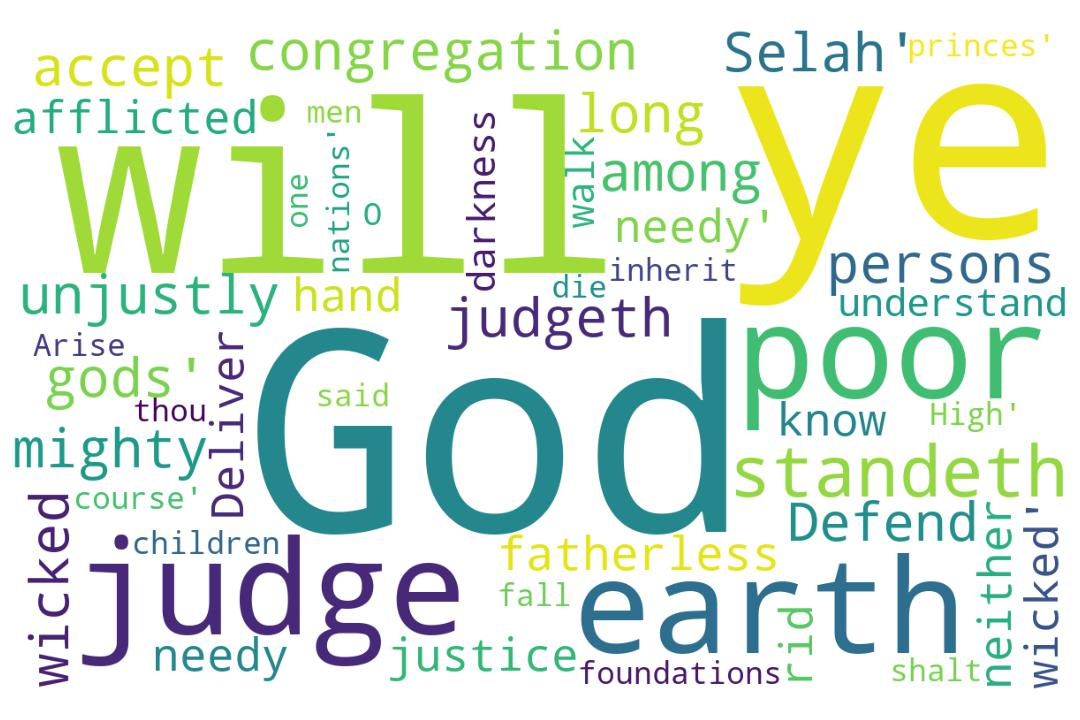
\includegraphics[width=\linewidth]{19OT-Psalms/Psalm82-WordCloud.jpg}
  \caption{Psalm 82 Word Cloud}
  \label{fig:Psalm 82 word Cloud}
\end{figure}

\marginpar{\scriptsize \centering \fcolorbox{bone}{lime}{\textbf{GOD IN CHARGE}}\\ (Psalm 81) \begin{compactenum}[I.][8]
   \item The \textbf{Realm of Leadership} \index[scripture]{Psalms!Psa 082:01}(Psa 82:1) 
    \item The \textbf{Ruin of a Leader} \index[scripture]{Psalms!Psa 082:02}(Psa 82:2) 
    \item The (Proper) \textbf{Regard of a Leader} \index[scripture]{Psalms!Psa 082:03}(Psa 82:3) 
    \item The \textbf{Rebuke of Leaders} \index[scripture]{Psalms!Psa 082:05}(Psa 82:5) 
    \item The \textbf{Reasons for Bad Leaders} \index[scripture]{Psalms!Psa 082:05}(Psa 82:5) 
    \item The \textbf{Return of THE LEADER} \index[scripture]{Psalms!Psa 082:08}(Psa 82:8) 
\end{compactenum}}

\marginpar{\scriptsize \centering \fcolorbox{bone}{yellow}{\textbf{COURT IN SESSION}}\\ (Psalm 81) \begin{compactenum}[I.][8]
   \item The \textbf{Delay} \index[scripture]{Psalms!Psa 082:02}(Psa 82:2) 
   \item The \textbf{Defense} \index[scripture]{Psalms!Psa 082:03}(Psa 82:3) 
   \item The \textbf{Deliverance} \index[scripture]{Psalms!Psa 082:04}(Psa 82:4) 
   \item The \textbf{Darkness} \index[scripture]{Psalms!Psa 082:05}(Psa 82:5) 
   \item The \textbf{Descent} \index[scripture]{Psalms!Psa 082:06}(Psa 82:6) 
   \item The \textbf{Death} \index[scripture]{Psalms!Psa 082:07}(Psa 82:7) 
   \item The \textbf{Disposing} \index[scripture]{Psalms!Psa 082:08}(Psa 82:8) 
\end{compactenum}}


\footnote{\textcolor[rgb]{0.00,0.25,0.00}{\hyperlink{PsalmsTOC}{Return to end of Table of Contents.}}}\footnote{\href{https://audiobible.com/bible/psalms_82.html}{\textcolor[cmyk]{0.99998,1,0,0}{Psalm 82 Audio}}}\textcolor[cmyk]{0.99998,1,0,0}{A Psalm of Asaph.}\\
\\
\textcolor[cmyk]{0.99998,1,0,0}{God standeth in the congregation of the mighty; he judgeth among the gods.}\footnote{\textbf{1 Kings 22:19} - And he said, Hear thou therefore the word of the LORD: I saw the LORD sitting on his throne, and all the host of heaven standing by him on his right hand and on his left.} %\footnote{But here, the spiritual truths give way to Biblical doctrines that are hard to hear, so those “dull of hearing” (Heb. 5:11) are now about to “bomb out” right and left. One will abort, one will miscarry, one will throw in the sponge, and another will move through the Psalm like a drugged sleep walker.\cite{Ruckman1992Psalms}}
[2] \textcolor[cmyk]{0.99998,1,0,0}{How long will ye judge unjustly, and accept the persons of the wicked? Selah.} %\footnote{“The congregation of the mighty” is not any congregation of earthly judges, and  when “he judgeth among the gods,” there is no reference to Israelite judges, any of Aaron’s seed, or anything else. Look at 1 Kings 22:19 for the Holy Spirit’s description of the “congregation of the mighty.” Verse 6 is what destroyed the spiritual sensibilities of Kroll, Duhm, Motyer, Clarke, Lange, Dummelow, Yates, Baethgen, Hengstenberg, and Charles Haddon Spurgeon. You will note that God often makes Charlie pay for his sin of leaning on the corrupt RV, at times, and occasionally aping Westcott and Hort by talking about “better renderings” and “better translations.” There is a price to pay for strutting like a peacock before the Holy Spirit. No man states the truth concerning the power and authority of the King James Bible any better than Spurgeon when he is in his right mind (see the Bible Believers’ Bulletin, September 1990), but alas, “all flesh is grass” and “all have sinned,” etc., so when Charlie tries to impress the stupid apostates of his day—who taught the faculties and staffs of every major Christian college and seminary everything they know—God puts him down as a candidate for blindness at a later date. This is one of those dates. That is the date line. It quickly eliminates every Nicolaitan who was trying to “bring out the intent of the original author” by “translating the Hebrew text in up to date language, so it might communicate to the receptor,” etc. (Interpretation: “He’s got a job that takes a lot of guts: he strings tennis rackets.”) \cite{Ruckman1992Psalms}}
[3] \textcolor[cmyk]{0.99998,1,0,0}{Defend the poor and fatherless: do justice to the afflicted and needy.}
[4] \textcolor[cmyk]{0.99998,1,0,0}{Deliver the poor and needy: rid \emph{them} out of the hand of the wicked.}
[5] \textcolor[cmyk]{0.99998,1,0,0}{They know not, neither will they understand; they walk on in darkness: all the foundations of the earth are out of course.}
[6] \textcolor[cmyk]{0.99998,1,0,0}{I have said, Ye \emph{are} gods; and all of you \emph{are} children of the most High.}
[7] \textcolor[cmyk]{0.99998,1,0,0}{But ye shall die like men, and fall like one of the princes.}\footnote{\textbf{Job 22:15-17} - Hast thou marked the old way which wicked men have trodden? 16 Which were cut down out of time, whose foundation was overflown with a flood: 17 Which said unto God, Depart from us: and what can the Almighty do for them?}\footnote{\textbf{2 Peter 2:4-5} - For if God spared not the angels that sinned, but cast them down to hell, and delivered them into chains of darkness, to be reserved unto judgment; 5 And spared not the old world, but saved Noah the eighth person, a preacher of righteousness, bringing in the flood upon the world of the ungodly;}% \footnote{You do not say: “I have said ye are cats, but ye shall die like cats.” You could say: “I have said ye are dogs, but ye will drown like fishes.” Two things that aren’t the same cannot be equated, so the scholars will have to “fix up” the “men” so they don’t stand in opposition to the “gods.” (That is what Scofield did with Genesis 6:2, so the “daughters of men” could simply be messing around with the “sons of men.” The text said “sons of God.”) This is fourth-grade English. The disjunctive conjunction (“but” vs. 7) shows us that we are not dealing with men; there are no human judges in verses 6–7. The contrast is between someone who might truly be a “god” but he will die like a man—not a “god.” Jamieson, Fausset, and Brown go to bat for every Biblecorrecting Nicolaitan at Liberty University and say that what the Holy Spirit meant to say in verse 7 was “not like any ordinary man.” This solves the problem for the Biblerejecting Fundamentalist who has no grasp of the Scriptures. “I have said you are above ordinary men, but you will die like ordinary men “; i.e., “I will tell you what the Scriptures should have said because as they are written it is impossible for me to understand them.” You see where this type of reasoning winds up? It winds up with “YOU need a different translation because the Holy Bible is impossible for YOU to understand. After all, if I, with my twenty five years of formal education, can’t understand it, how could YOU possibly understand it? Here! Buy this Nutty Imbecile’s Version (NIV). Cash, check, or money order!” See how it’s done? The judges in Genesis 6 corrupted the entire earth with their decisions. They made decisions worse than the ones made by the “nine old men” since 1933. These supernatural “gods” are identified as “gods” in the following places: Genesis 3:5; Exodus 15:11; Psalm 86:8, 95:3, 136:2 (Note THAT one! lmgine thinking those “gods” are Israelite judges!), and Jeremiah 10:11. They are called “the sons of God” in Job 38:7 and Genesis 6:2, so the only way Scofield could remove “children of the most High” from Psalm 82:6 was to pretend that the “gods” were NOT literally “the sons of God.” They were the “sons of Seth”! Had enough of “higher scholarship”? Is this enough from the “recognized scholars” whose “loyalty” to lost pieces of paper is “unquestioned”? Gotta belly full yet, or are you like the little boy who was told “If you eat one more bite, you are going to bust wide open”? He replied, “Please pass the cake and everybody stand back. “ The “gods” have been here before and will be here again. Idols are the mementos that man has used since the flood to commemorate their presence (see Isa. 44:10; Ps. 96:5, 97:7). They came down “in the likeness of men” according to the New Testament (Acts 14:11), so every angel in the Bible appears as a young man (Judg. 13:6; Gen. 19:5; Acts 1:10; Luke 24:4, etc.). Scofield got rid of them again by saying “angels are sexless.” But when he says “ye shall die like men,” he meant they would drown in the flood (2 Pet. 2:4–5; Job 22:15– 17), and so they did. At the time they were judging, Enoch was prophesying the Second Coming of Jesus Christ (see Jude 14). There is a chance that this Psalm may be a pre Deluge Psalm written by Enoch (see remarks under Ps. 90). All the commentators “blew it.” It is evident that once a man begins to mess with the King James text that the Author of Scripture begins to mess with his mind, and pretty soon he cannot get the simplest doctrinal and prophetic truths in order. This statement is proved the moment some blockhead on the faculty at Bob Jones, PCC, Santa Rosa, BBC, or Tennessee Temple tries to cover up his infidelity. We will cite an A 1 example, honed to perfection at Liberty University. Having been told that “all the foundations of the earth are out of course” (vs. 5)—which matches Isaiah 24:19–20—Kroll, of Liberty University, alters them to “the fabric of the nation.” (So help me, Delitzsch and Keil, that is what Lynchburg did with “the Hebrew text.”) ``Yet in the highly poetic language of the Psalm...when the fundamental basis of society, the very principles of morality, are not followed by the judges, the very fabric of the nation is shaken.'' Go sit on a tack. That is modern, “militant Fundamentalist” scholarship in 1992. It is a combination of stupidity, unbelief, arrogance, blindness, and equivocation wrapped up in one neat ball of piety and propagated by men who “don’t like Brother Ruckman’s language.” (I hope to God they don’t, and I hope to God they never will.) \cite{Ruckman1992Psalms}}
[8] \textcolor[cmyk]{0.99998,1,0,0}{Arise, O God, judge the earth: for thou shalt inherit all nations.} %\footnote{There it goes again, in case you missed the “Selah.” But at Liberty University they can’t find EITHER expression in ANY version. Kroll (absolutely spaced out) says that “Arise, O God” is just a “metaphor taken from the common gesture of judges who sit as they hear a case and rise up to pronounce a sentence.” No, that is exactly what the expression didn’t mean one time anywhere in the entire Bible. See Psalm 3:7, 7:6, 9:19, 10:12, 12:5, 17:13, 44:23, 26, 68:1, and 74:22. It wasn’t a “metaphor” one time out of ten. Trust Lynchburg to steal your money as well as your Bible. “For thou shalt inherit all nations” gave you the third clue as to the time, and Kroll still missed it. He had to apply the second half of verse 8 to the Second Advent because he was Premillennial, but being carnal (as well as stupid), he had to limit the first half of the verse to human judges before the Church Age. He, as everyone of his peers, ignored the fact that the ``gods'' will be here in the Tribulation, and they will be reigning not only as kings but as absolute authorities over all judicial matters on earth (Rev. 17:12). They will be in the same position as in Genesis 6:1--6. (Note the word “mighty,” as in Ps. 82:1.) When Christ applied the verse to human judges to prove His own deity (John 10:34--36), He knocked every translator, every reviser, every commentator, and every ``exegete'' slap out of the rink. At no time did God ever say “all of you Israelite judges are children of the most High.” To tell the truth, none of them were; not even the saved ones. The judges in Israel were Levites (Mal. 2:4, 7–8; Deut. 1:16, 21:5), and not one of them was a “child of God.” When John uses the expression (John 11:52), he uses it in a Jewish sense that was not doctrinal. Jesus Christ Himself allows that the Jews of that time were not only NOT the “children of God” (John 8:42--44), they were not even the children of Abraham (John 8:39). That isn’t all: “all the foundations of the earth” (vs. 5) were NOT “out of course” at anytime between Asaph and Paul, and they are not now, nor were they when Moses appointed human judges over Israel (Exodus 18:22, 25; Num. 11:16--17). Someone is “off their trolley” again; they have “one oar in the water.” The problem came from Exodus 22:28. With this and John 10:34, the Bible-correcting apostates took the liberty to throw out the entire context of Psalm 82, since they couldn’t understand it. The context (vss. 1, 5–6, 8) was the Second Advent, and the type was “the days of Noah,” for there the “gods” drowned like “men” (see vs. 7), at least according to 2 Peter 3:6; Jude 6; Job 22:16;  and Revelation 20:13 in the English text. There is nothing like Elizabethan English to make a debacle out of a seminary; especially if it is a bunch of book mad stuffed shirts who think the sun rises and sets on ``plenary, verbally inspired, original autographs.'' (A duck is a bird that walks like he has been riding a horse all day.) Dual application: The judges in Israel could be ``gods'' in the sense that Moses was a “god” to Pharaoh and Aaron (Exod. 7:1). You can be a ``son'' of God because you represent THE Son of God. (The Pope is not shy in the least; he simply applies God’s titles to himself, John 17:11.) The human judges could judge ``the poor and fatherless...the afflicted and needy...the poor and needy,'' so they acted as gods for these people. Final Authority. Get it? You got it yet? Christ merely quotes the passage to show that they have no right to accuse Him of claiming to be something that He is not. He doesn’t tell you one thing about the Psalm or what the Psalm was dealing with. So the Nicolaitans—who have been correcting the Psalms now for ten to three hundred years—can’t find out what is going on. When Christ says that it is written in the Law ``I said, ye are gods,'' the ``ye'' doesn’t have anything to do with anyone to whom He is talking who got ``the word of God.'' The ``ye'' was a reference to angels from Genesis 6 who will show up in the Tribulation. \cite{Ruckman1992Psalms}}


\index[NWIV]{13!Psalms!Psa 82:1}\index[AWIP]{God!Psalms!Psa 82:1}\index[AWIP]{standeth!Psalms!Psa 82:1}\index[AWIP]{in!Psalms!Psa 82:1}\index[AWIP]{the!Psalms!Psa 82:1}\index[AWIP]{the!Psalms!Psa 82:1 (2)}\index[AWIP]{the!Psalms!Psa 82:1 (3)}\index[AWIP]{congregation!Psalms!Psa 82:1}\index[AWIP]{of!Psalms!Psa 82:1}\index[AWIP]{mighty!Psalms!Psa 82:1}\index[AWIP]{he!Psalms!Psa 82:1}\index[AWIP]{judgeth!Psalms!Psa 82:1}\index[AWIP]{among!Psalms!Psa 82:1}\index[AWIP]{gods!Psalms!Psa 82:1}

\index[NWIV]{14!Psalms!Psa 82:2}\index[AWIP]{How!Psalms!Psa 82:2}\index[AWIP]{long!Psalms!Psa 82:2}\index[AWIP]{will!Psalms!Psa 82:2}\index[AWIP]{ye!Psalms!Psa 82:2}\index[AWIP]{judge!Psalms!Psa 82:2}\index[AWIP]{unjustly!Psalms!Psa 82:2}\index[AWIP]{and!Psalms!Psa 82:2}\index[AWIP]{accept!Psalms!Psa 82:2}\index[AWIP]{the!Psalms!Psa 82:2}\index[AWIP]{the!Psalms!Psa 82:2 (2)}\index[AWIP]{persons!Psalms!Psa 82:2}\index[AWIP]{of!Psalms!Psa 82:2}\index[AWIP]{wicked?!Psalms!Psa 82:2}\index[AWIP]{Selah!Psalms!Psa 82:2}

\index[NWIV]{12!Psalms!Psa 82:3}\index[AWIP]{Defend!Psalms!Psa 82:3}\index[AWIP]{the!Psalms!Psa 82:3}\index[AWIP]{the!Psalms!Psa 82:3 (2)}\index[AWIP]{poor!Psalms!Psa 82:3}\index[AWIP]{and!Psalms!Psa 82:3}\index[AWIP]{and!Psalms!Psa 82:3 (2)}\index[AWIP]{fatherless!Psalms!Psa 82:3}\index[AWIP]{do!Psalms!Psa 82:3}\index[AWIP]{justice!Psalms!Psa 82:3}\index[AWIP]{to!Psalms!Psa 82:3}\index[AWIP]{afflicted!Psalms!Psa 82:3}\index[AWIP]{needy!Psalms!Psa 82:3}

\index[NWIV]{14!Psalms!Psa 82:4}\index[AWIP]{Deliver!Psalms!Psa 82:4}\index[AWIP]{the!Psalms!Psa 82:4}\index[AWIP]{the!Psalms!Psa 82:4 (2)}\index[AWIP]{the!Psalms!Psa 82:4 (3)}\index[AWIP]{poor!Psalms!Psa 82:4}\index[AWIP]{and!Psalms!Psa 82:4}\index[AWIP]{needy!Psalms!Psa 82:4}\index[AWIP]{rid!Psalms!Psa 82:4}\index[AWIP]{\emph{them}!Psalms!Psa 82:4}\index[AWIP]{out!Psalms!Psa 82:4}\index[AWIP]{of!Psalms!Psa 82:4}\index[AWIP]{of!Psalms!Psa 82:4 (2)}\index[AWIP]{hand!Psalms!Psa 82:4}\index[AWIP]{wicked!Psalms!Psa 82:4}\index[AWIP]{\emph{them}!Psalms!Psa 82:4}

\index[NWIV]{22!Psalms!Psa 82:5}\index[AWIP]{They!Psalms!Psa 82:5}\index[AWIP]{know!Psalms!Psa 82:5}\index[AWIP]{not!Psalms!Psa 82:5}\index[AWIP]{neither!Psalms!Psa 82:5}\index[AWIP]{will!Psalms!Psa 82:5}\index[AWIP]{they!Psalms!Psa 82:5}\index[AWIP]{they!Psalms!Psa 82:5 (2)}\index[AWIP]{understand!Psalms!Psa 82:5}\index[AWIP]{walk!Psalms!Psa 82:5}\index[AWIP]{on!Psalms!Psa 82:5}\index[AWIP]{in!Psalms!Psa 82:5}\index[AWIP]{darkness!Psalms!Psa 82:5}\index[AWIP]{all!Psalms!Psa 82:5}\index[AWIP]{the!Psalms!Psa 82:5}\index[AWIP]{the!Psalms!Psa 82:5 (2)}\index[AWIP]{foundations!Psalms!Psa 82:5}\index[AWIP]{of!Psalms!Psa 82:5}\index[AWIP]{of!Psalms!Psa 82:5 (2)}\index[AWIP]{earth!Psalms!Psa 82:5}\index[AWIP]{are!Psalms!Psa 82:5}\index[AWIP]{out!Psalms!Psa 82:5}\index[AWIP]{course!Psalms!Psa 82:5}

\index[NWIV]{16!Psalms!Psa 82:6}\index[AWIP]{I!Psalms!Psa 82:6}\index[AWIP]{have!Psalms!Psa 82:6}\index[AWIP]{said!Psalms!Psa 82:6}\index[AWIP]{Ye!Psalms!Psa 82:6}\index[AWIP]{\emph{are}!Psalms!Psa 82:6}\index[AWIP]{\emph{are}!Psalms!Psa 82:6 (2)}\index[AWIP]{gods!Psalms!Psa 82:6}\index[AWIP]{and!Psalms!Psa 82:6}\index[AWIP]{all!Psalms!Psa 82:6}\index[AWIP]{of!Psalms!Psa 82:6}\index[AWIP]{of!Psalms!Psa 82:6 (2)}\index[AWIP]{you!Psalms!Psa 82:6}\index[AWIP]{children!Psalms!Psa 82:6}\index[AWIP]{the!Psalms!Psa 82:6}\index[AWIP]{most!Psalms!Psa 82:6}\index[AWIP]{High!Psalms!Psa 82:6}\index[AWIP]{\emph{are}!Psalms!Psa 82:6}\index[AWIP]{\emph{are}!Psalms!Psa 82:6 (2)}

\index[NWIV]{13!Psalms!Psa 82:7}\index[AWIP]{But!Psalms!Psa 82:7}\index[AWIP]{ye!Psalms!Psa 82:7}\index[AWIP]{shall!Psalms!Psa 82:7}\index[AWIP]{die!Psalms!Psa 82:7}\index[AWIP]{like!Psalms!Psa 82:7}\index[AWIP]{like!Psalms!Psa 82:7 (2)}\index[AWIP]{men!Psalms!Psa 82:7}\index[AWIP]{and!Psalms!Psa 82:7}\index[AWIP]{fall!Psalms!Psa 82:7}\index[AWIP]{one!Psalms!Psa 82:7}\index[AWIP]{of!Psalms!Psa 82:7}\index[AWIP]{the!Psalms!Psa 82:7}\index[AWIP]{princes!Psalms!Psa 82:7}

\index[NWIV]{12!Psalms!Psa 82:8}\index[AWIP]{Arise!Psalms!Psa 82:8}\index[AWIP]{O!Psalms!Psa 82:8}\index[AWIP]{God!Psalms!Psa 82:8}\index[AWIP]{judge!Psalms!Psa 82:8}\index[AWIP]{the!Psalms!Psa 82:8}\index[AWIP]{earth!Psalms!Psa 82:8}\index[AWIP]{for!Psalms!Psa 82:8}\index[AWIP]{thou!Psalms!Psa 82:8}\index[AWIP]{shalt!Psalms!Psa 82:8}\index[AWIP]{inherit!Psalms!Psa 82:8}\index[AWIP]{all!Psalms!Psa 82:8}\index[AWIP]{nations!Psalms!Psa 82:8}


\section{Psalm 82 Outlines}

\subsection{My Outlines}

\subsubsection{God in Charge}

\index[speaker]{Keith Anthony!Psalm 082 (God in Charge)}
\index[series]{Psalms (Keith Anthony)!Psalm 082 (God in Charge)}
\index[date]{2016/08/26!Psalm 082 (God in Charge) (Keith Anthony)}

\begin{compactenum}[I.][7]
    \item The \textbf{Realm of Leadership} \index[scripture]{Psalms!Psa 082:01}(Psa 82:1) 
    \item The \textbf{Ruin of a Leader} \index[scripture]{Psalms!Psa 082:02}(Psa 82:2) 
    \item The (Proper) \textbf{Regard of a Leader} \index[scripture]{Psalms!Psa 082:03}(Psa 82:3) 
    \item The \textbf{Rebuke of Leaders} \index[scripture]{Psalms!Psa 082:05}(Psa 82:5) 
    \item The \textbf{Reasons for Bad Leaders} \index[scripture]{Psalms!Psa 082:05}(Psa 82:5) 
    \item The \textbf{Return of THE LEADER} \index[scripture]{Psalms!Psa 082:08}(Psa 82:8) 
\end{compactenum}


\subsubsection{Court in Session}

\index[speaker]{Keith Anthony!Psalm 082 (Court in Session)}
\index[series]{Psalms (Keith Anthony)!Psalm 082 (Court in Session)}
\index[date]{2020/09/09!Psalm 082 (Court in Session) (Keith Anthony)}

\begin{compactenum}[I.][8]
   \item The \textbf{Delay} \index[scripture]{Psalms!Psa 082:02}(Psa 82:2) 
   \item The \textbf{Defense} \index[scripture]{Psalms!Psa 082:03}(Psa 82:3) 
   \item The \textbf{Deliverance} \index[scripture]{Psalms!Psa 082:04}(Psa 82:4) 
   \item The \textbf{Darkness} \index[scripture]{Psalms!Psa 082:05}(Psa 82:5) 
   \item The \textbf{Descent} \index[scripture]{Psalms!Psa 082:06}(Psa 82:6) 
   \item The \textbf{Death} \index[scripture]{Psalms!Psa 082:07}(Psa 82:7) 
   \item The \textbf{Disposing} \index[scripture]{Psalms!Psa 082:08}(Psa 82:8) 
\end{compactenum}

\subsection{Outlines from Others}


\section{Psalm 82 Comments}

\subsection{Numeric Nuggets}
There are 13 words in verses 1 and 7, along with 13 unique words in verse 2. The 13$^{th}$ word in the psalm is ``gods.''  The 26$^{th}$ (2 x 13) word in the psalm is ``wicked.'' The 13$^{th}$ word in verse 7 is ``princes.''

\subsection{Introduction}
The context of Psalm 82 (as seen in verses 1, 5-6, and 8) is the Second Advent of Jesus Christ and these mysterious creatures called ``gods''.  Does the psalm actually  acknowledge that there are other deities with and despite whom the Lord works and over whom He presides and rules? 

Hints to the context of the psalm include the use of the word ``Selah'' in verse 2, a call for judgment against the wicked, a description of the ``foundations of the earth'', a mention of ``gods'', and a mention of the inheritance of God in verse 8. In the middle of the conflict, the victims, are the poor and fatherless, and the afflicted and needy, the poor and needy in verses 3 and 4. 

The ``fatherless' are first seen in Exodus 22:22-24, as a group which has a unique concern of the Lord.\footnote{\textbf{Exodus 22:22-24} - Ye shall not afflict any widow, or fatherless child. [23] If thou afflict them in any wise, and they cry at all unto me, I will surely hear their cry; [24 ] And my wrath shall wax hot, and I will kill you with the sword; and your wives shall be widows, and your children fatherless.} They are last seen in scripture in the tribulation context in James 1:27.\footnote{\textbf{James 1:27} - Pure religion and undefiled before God and the Father is this, To visit the fatherless and widows in their affliction, and to keep himself unspotted from the world.} The ``fatherless' are found in, notably, 13 books in the AV. 

Psalm 82 presents an accusation against God. He is judging among the ``gods'' but judging unjustly. The persons of the wicked are afflicting people and are apparently being allowed to do it.  But the situation is temporary, and the godly order of things will be restored.

\subsection{Psalm 82:1}
The meaning of ``the wicked'' is established in Job 8:22 (among the 103 references in the AV) with a specific dwelling place. They are the children of the ``wicked one'' in Matthew 13:38.\footnote{\textbf{Matthew 13:38} - he field is the world; the good seed are the children of the kingdom; but the tares are the children of the wicked one;} They are ``children of pride'' in Job 41:34.\footnote{\textbf{Job 41:34} - He beholdeth all high things: he is a king over all the children of pride.} The word ``mighty'' in the verse makes an immediate connection back to the mighty men in Genesis 6:4.\footnote{\textbf{Genesis 6:4} - There were giants in the earth in those days; and also after that, when the sons of God came in unto the daughters of men, and they bare children to them, the same became mighty men which were of old, men of renown.} Another connection is to Nimrod in Genesis 10.\footnote{\textbf{Genesis 10:8-9} - And Cush begat Nimrod: he began to be a mighty one in the earth. [ 9] He was a mighty hunter before the LORD: wherefore it is said, Even as Nimrod the mighty hunter before the LORD.}

The short answer to the question posed earlier in ``yes.'' 

\subsection{Psalm 82:2}
The question ``how long'' is one of the famous questions contained in scripture, asked first to Pharaoh In Exodus 10:3, and last in the Great tribulation in Revelation 6:2.\footnote{\textbf{Revelation 6:2} - And they cried with a loud voice, saying, How long, O Lord, holy and true, dost thou not judge and avenge our blood on them that dwell on the earth?} ``Unjustly'' is used twice, here and in Isaiah 26:16, describing favour and mercy being shown to the wicked in an effort to unsuccessfully stimulate repentance.\footnote{\textbf{Isaiah 26:10} - Let favour be shewed to the wicked, yet will he not learn righteousness: in the land of uprightness will he deal unjustly, and will not behold the majesty of the LORD.}

\subsection{Psalm 82:5}
The phrase ``most High'' is first used in the story of Abraham and Melchisedek in Genesis 14.\footnote{\textbf{Genesis 14:18-22} - And Melchizedek king of Salem brought forth bread and wine: and he was the priest of the most high God. [19] And he blessed him, and said, Blessed be Abram of the most high God, possessor of heaven and earth: [20 ]And blessed be the most high God, which hath delivered thine enemies into thy hand. And he gave him tithes of all. [21] And the king of Sodom said unto Abram, Give me the persons, and take the goods to thyself. [22] And Abram said to the king of Sodom, I have lift up mine hand unto the LORD, the most high God, the possessor of heaven and earth, }


\subsection{Psalm 82:6, 7}
Who are these ``gods''? For starters, verse 7 distinguishes them from ``men'' and from ``princes.'' It may well be that this psalm may be a pre-Deluxe psalm, composed by Enoch. This is supported by the fact that the death referred to was the be Noah's flood. The ``gods'' die like mean because they have ``given up their first estate'' spoken of in Jude 6 and 7.\footnote{\textbf{Jude 6,7} - And the angels which kept not their first estate, but left their own habitation, he hath reserved in everlasting chains under darkness unto the judgment of the great day. [7] Even as Sodom and Gomorrha, and the cities about them in like manner, giving themselves over to fornication, and going after strange flesh, are set forth for an example, suffering the vengeance of eternal fire.} These are the ``sons of God'' in Genesis 6, evidently judges, and judging badly. For other evidence, see Genesis 3:5.\footnote{\textbf{Genesis 3:5} - For God doth know that in the day ye eat thereof, then your eyes shall be opened, and ye shall be as gods, knowing good and evil.} See Exodus 15:11.\footnote{\textbf{Exodus 15:11} - Who is like unto thee, O LORD, among the gods? who is like thee, glorious in holiness, fearful in praises, doing wonders?} See Psalm 86:8, 95:3,and 136:2.\footnote{\textbf{Psalm 86:8} - (Psalms 86:8) "Among the gods there is none like unto thee, O Lord; neither are there any works like unto thy works."}\footnote{\textbf{Psalm 95:3} - For the LORD is a great God, and a great King above all gods.}\footnote{\textbf{Psalm 136:2} - O give thanks unto the God of gods: for his mercy endureth for ever.}

The verses confront the standard interpretation that these ``gods'' were human judges, given the titles as God's representatives. The standard view is the same nonsense as the ``godly line of Seth'' in Genesis 4 and 5, a view regarded as absurd by John Calvin.

The ``gods'' are among the ``principalities and powers'' of Ephesians 6:12.\footnote{\textbf{Ephesians 6:12} - For we wrestle not against flesh and blood, but against principalities, against powers, against the rulers of the darkness of this world, against spiritual wickedness in high places.}

\subsection{Psalm 82:8}
The phrase ``Arise, O God'' or ``Arise, O LORD'' is found 9 times in scripture, and is anything but symbolic or metaphoric. In each instance, it refers to judgment and deliverance. Notably, the bookends for the references refer to thy resting place or rest, pointing to the Millennium:
\begin{compactenum}[1.]
	\item  \textbf{2 Chronicles 6:41} Now therefore arise, O LORD God, into thy resting place, thou, and the ark of thy strength: let thy priests, O LORD God, be clothed with salvation, and let thy saints rejoice in goodness.
	\item \textbf{Psalm 3:7} Arise, O LORD; save me, O my God: for thou hast smitten all mine enemies upon the cheek bone; thou hast broken the teeth of the ungodly.
	\item \textbf{Psalm 7:6} Arise, O LORD, in thine anger, lift up thyself because of the rage of mine enemies: and awake for me to the judgment that thou hast commanded
	\item \textbf{Psalm 9:19}  Arise, O LORD; let not man prevail: let the heathen be judged in thy sight.
	\item \textbf{Psalm 10:12} Arise, O LORD; O God, lift up thine hand: forget not the humble.
	\item \textbf{Psalm 17:13} Arise, O LORD, disappoint him, cast him down: deliver my soul from the wicked, which is thy sword: 
	\item \textbf{Psalm 74:22} Arise, O God, plead thine own cause: remember how the foolish man reproacheth thee daily. 
	\item \textbf{Psalm 82:8}  Arise, O God, judge the earth: for thou shalt inherit all nations.
	\item \textbf{Psalm 132:8}Arise, O LORD, into thy rest; thou, and the ark of thy strength.
\end{compactenum}
\subsection{Psalm 82 Repeated Phrases}


%%%%%%%%%%
%%%%%%%%%%
\normalsize
 
\begin{center}
\begin{longtable}{|p{3.0in}|p{0.5in}|}
\caption[Psalm8 2 Repeated Phrases]{Psalm 82 Repeated Phrases}\label{table:Repeated Phrases Psalm 82} \\
\hline \multicolumn{1}{|c|}{\textbf{Phrase}} & \multicolumn{1}{c|}{\textbf{Frequency}} \\ \hline 
\endfirsthead
 
\multicolumn{2}{c}
{{\bfseries \tablename\ \thetable{} -- continued from previous page}} \\  
\hline \multicolumn{1}{|c|}{\textbf{Phrase}} & \multicolumn{1}{c|}{\textbf{Frequency}} \\ \hline 
\endhead
 
\hline \multicolumn{2}{c}{{ }} \\ \hline
\endfoot 
of the & 7\\ \hline 
\end{longtable}
\end{center}



%%%%%%%%%%
%%%%%%%%%%



\section{Psalm 82 Statistics}

%%%%%%%%%%%%%%%%%%%%%%%%%%%
%%%%% Word Statistics
%%%%%%%%%%%%%%%%%%%%%%%%%%


\normalsize



\subsection{Chapter Word Statistics}


%%%%%%%%%%
%%%%%%%%%%
 
\begin{center}
\begin{longtable}{l|c|c|c|c}
\caption[Stats for Psalm 82]{Stats for Psalm 82} \label{table:Stats for Psalm 82} \\ 
\hline \multicolumn{1}{|c|}{\textbf{Verse(s)}} & \multicolumn{1}{|c|}{\textbf{Count}} & \multicolumn{1}{|c|}{\textbf{Unique}} & \multicolumn{1}{|c|}{\textbf{Italics}} & \multicolumn{1}{|c|}{\textbf{Uniq Italic}}  \\ \hline 
\endfirsthead
 
\multicolumn{5}{c}
{{\bfseries \tablename\ \thetable{} -- continued from previous page}} \\  
\hline \multicolumn{1}{|c|}{\textbf{Verse(s)}} & \multicolumn{1}{|c|}{\textbf{Count}} & \multicolumn{1}{|c|}{\textbf{Unique}} & \multicolumn{1}{|c|}{\textbf{Italics}} & \multicolumn{1}{|c|}{\textbf{Uniq Italic}}  \\ \hline 
\endhead
 
\hline \multicolumn{5}{|r|}{{Continued if needed}} \\ \hline
\endfoot 
1 & 13 & 11 & 0 & 0\\ \hline
2 & 14 & 13 & 0 & 0\\ \hline
3 & 12 & 10 & 0 & 0\\ \hline
4 & 14 & 11 & 1 & 1\\ \hline
5 & 22 & 19 & 0 & 0\\ \hline
6 & 16 & 14 & 2 & 1\\ \hline
7 & 13 & 12 & 0 & 0\\ \hline
8 & 12 & 12 & 0 & 0\\ \hline
\hline \hline
Total & 116 & 73 & 3 & 2



\end{longtable}
\end{center}

%%%%%%%%%%
%%%%%%%%%%
 
\subsection{Words by Frequency}

\begin{center}
\begin{longtable}{l|r}
\caption[Word Frequencies in Psalm 82]{Word Frequencies in Psalm 82} \label{table:WordsIn-Psalm-82} \\ 
\hline \multicolumn{1}{|c|}{\textbf{Word}} & \multicolumn{1}{c|}{\textbf{Frequency}} \\ \hline 
\endfirsthead
 
\multicolumn{2}{c}
{{\bfseries \tablename\ \thetable{} -- continued from previous page}} \\ 
\hline \multicolumn{1}{|c|}{\textbf{Word}} & \multicolumn{1}{c|}{\textbf{Frequency}} \\ \hline 
\endhead
 
\hline \multicolumn{2}{|r|}{{Continued if needed}} \\ \hline
\endfoot
 
\hline \hline
\endlastfoot
the & 15 \\ \hline
of & 9 \\ \hline
and & 6 \\ \hline
all & 3 \\ \hline
God & 2 \\ \hline
in & 2 \\ \hline
gods & 2 \\ \hline
will & 2 \\ \hline
ye & 2 \\ \hline
judge & 2 \\ \hline
wicked & 2 \\ \hline
poor & 2 \\ \hline
needy & 2 \\ \hline
out & 2 \\ \hline
they & 2 \\ \hline
earth & 2 \\ \hline
\emph{are} & 2 \\ \hline
like & 2 \\ \hline
standeth & 1 \\ \hline
congregation & 1 \\ \hline
mighty & 1 \\ \hline
he & 1 \\ \hline
judgeth & 1 \\ \hline
among & 1 \\ \hline
How & 1 \\ \hline
long & 1 \\ \hline
unjustly & 1 \\ \hline
accept & 1 \\ \hline
persons & 1 \\ \hline
Selah & 1 \\ \hline
Defend & 1 \\ \hline
fatherless & 1 \\ \hline
do & 1 \\ \hline
justice & 1 \\ \hline
to & 1 \\ \hline
afflicted & 1 \\ \hline
Deliver & 1 \\ \hline
rid & 1 \\ \hline
\emph{them} & 1 \\ \hline
hand & 1 \\ \hline
They & 1 \\ \hline
know & 1 \\ \hline
not & 1 \\ \hline
neither & 1 \\ \hline
understand & 1 \\ \hline
walk & 1 \\ \hline
on & 1 \\ \hline
darkness & 1 \\ \hline
foundations & 1 \\ \hline
are & 1 \\ \hline
course & 1 \\ \hline
I & 1 \\ \hline
have & 1 \\ \hline
said & 1 \\ \hline
Ye & 1 \\ \hline
you & 1 \\ \hline
children & 1 \\ \hline
most & 1 \\ \hline
High & 1 \\ \hline
But & 1 \\ \hline
shall & 1 \\ \hline
die & 1 \\ \hline
men & 1 \\ \hline
fall & 1 \\ \hline
one & 1 \\ \hline
princes & 1 \\ \hline
Arise & 1 \\ \hline
O & 1 \\ \hline
for & 1 \\ \hline
thou & 1 \\ \hline
shalt & 1 \\ \hline
inherit & 1 \\ \hline
nations & 1 \\ \hline
\end{longtable}
\end{center}



\normalsize



\subsection{Words Alphabetically}

\begin{center}
\begin{longtable}{l|r}
\caption[Word Alphabetically in Psalm 82]{Word Alphabetically in Psalm 82} \label{table:WordsIn-Psalm-82} \\ 
\hline \multicolumn{1}{|c|}{\textbf{Word}} & \multicolumn{1}{c|}{\textbf{Frequency}} \\ \hline 
\endfirsthead
 
\multicolumn{2}{c}
{{\bfseries \tablename\ \thetable{} -- continued from previous page}} \\ 
\hline \multicolumn{1}{|c|}{\textbf{Word}} & \multicolumn{1}{c|}{\textbf{Frequency}} \\ \hline 
\endhead
 
\hline \multicolumn{2}{|r|}{{Continued if needed}} \\ \hline
\endfoot
 
\hline \hline
\endlastfoot
Arise & 1 \\ \hline
But & 1 \\ \hline
Defend & 1 \\ \hline
Deliver & 1 \\ \hline
God & 2 \\ \hline
High & 1 \\ \hline
How & 1 \\ \hline
I & 1 \\ \hline
O & 1 \\ \hline
Selah & 1 \\ \hline
They & 1 \\ \hline
Ye & 1 \\ \hline
\emph{are} & 2 \\ \hline
\emph{them} & 1 \\ \hline
accept & 1 \\ \hline
afflicted & 1 \\ \hline
all & 3 \\ \hline
among & 1 \\ \hline
and & 6 \\ \hline
are & 1 \\ \hline
children & 1 \\ \hline
congregation & 1 \\ \hline
course & 1 \\ \hline
darkness & 1 \\ \hline
die & 1 \\ \hline
do & 1 \\ \hline
earth & 2 \\ \hline
fall & 1 \\ \hline
fatherless & 1 \\ \hline
for & 1 \\ \hline
foundations & 1 \\ \hline
gods & 2 \\ \hline
hand & 1 \\ \hline
have & 1 \\ \hline
he & 1 \\ \hline
in & 2 \\ \hline
inherit & 1 \\ \hline
judge & 2 \\ \hline
judgeth & 1 \\ \hline
justice & 1 \\ \hline
know & 1 \\ \hline
like & 2 \\ \hline
long & 1 \\ \hline
men & 1 \\ \hline
mighty & 1 \\ \hline
most & 1 \\ \hline
nations & 1 \\ \hline
needy & 2 \\ \hline
neither & 1 \\ \hline
not & 1 \\ \hline
of & 9 \\ \hline
on & 1 \\ \hline
one & 1 \\ \hline
out & 2 \\ \hline
persons & 1 \\ \hline
poor & 2 \\ \hline
princes & 1 \\ \hline
rid & 1 \\ \hline
said & 1 \\ \hline
shall & 1 \\ \hline
shalt & 1 \\ \hline
standeth & 1 \\ \hline
the & 15 \\ \hline
they & 2 \\ \hline
thou & 1 \\ \hline
to & 1 \\ \hline
understand & 1 \\ \hline
unjustly & 1 \\ \hline
walk & 1 \\ \hline
wicked & 2 \\ \hline
will & 2 \\ \hline
ye & 2 \\ \hline
you & 1 \\ \hline
\end{longtable}
\end{center}



\normalsize



\subsection{Word Lengths in Chapter}
\normalsize
\begin{longtable}{l|p{3.75in}}
\caption[Words by Length in Psalm 82]{Words by Length in Psalm 82} \label{table:WordsIn-Psalm-82} \\ 
\hline \multicolumn{1}{|c|}{\textbf{Length}} & \multicolumn{1}{c|}{\textbf{Words}} \\ \hline 
\endfirsthead
 
\multicolumn{2}{c}
{{\bfseries \tablename\ \thetable{} -- continued from previous page}} \\ 
\hline \multicolumn{1}{|c|}{\textbf{Length}} & \multicolumn{1}{c|}{\textbf{Words}} \\ \hline 
\endhead
 
\hline \multicolumn{2}{|r|}{{Continued if needed}} \\ \hline
\endfoot
 
\hline \hline
\endlastfoot
1 & I, O \\ \hline
2 & in, of, he, ye, do, to, on, Ye \\ \hline
3 & God, the, How, and, rid, out, not, all, are, \emph{are}, you, But, die, men, one, for \\ \hline
4 & gods, long, will, poor, \emph{them}, hand, They, know, they, walk, have, said, most, High, like, fall, thou \\ \hline
5 & among, judge, Selah, needy, earth, shall, Arise, shalt \\ \hline
6 & mighty, accept, wicked, Defend, course \\ \hline
7 & judgeth, persons, justice, Deliver, neither, princes, inherit, nations \\ \hline
8 & standeth, unjustly, darkness, children \\ \hline
9 & afflicted \\ \hline
10 & fatherless, understand \\ \hline
11 & foundations \\ \hline
12 & congregation \\ \hline
\end{longtable}






%%%%%%%%%%
%%%%%%%%%%
 



%%%%%%%%%%
%%%%%%%%%%
\subsection{Verses with 13 Words in Chapter}
\normalsize
\begin{longtable}{l|p{3.75in}}
\caption[Verses with 13 Words  in Psalm 82]{Verses with 13 Words  in Psalm 82} \label{table:Verses with 13 Words in-Psalm-82} \\ 
\hline \multicolumn{1}{|c|}{\textbf{Reference}} & \multicolumn{1}{c|}{\textbf{Verse}} \\ \hline 
\endfirsthead
 
\multicolumn{2}{c}
{{\bfseries \tablename\ \thetable{} -- continued from previous page}} \\ 
\hline \multicolumn{1}{|c|}{\textbf{Reference}} & \multicolumn{1}{c|}{\textbf{Verse}} \\ \hline 
\endhead
 
\hline \multicolumn{2}{|r|}{{Continued if needed}} \\ \hline
\endfoot
 
\hline \hline
\endlastfoot
Psalms 082:1 & God standeth in the congregation of the mighty; he judgeth among the gods. \\ \hline
Psalms 082:7 & But ye shall die like men, and fall like one of the princes. \\ \hline
\end{longtable}






%%%%%%%%%%
%%%%%%%%%%

\chapter{Proverb 22}

\begin{figure}
  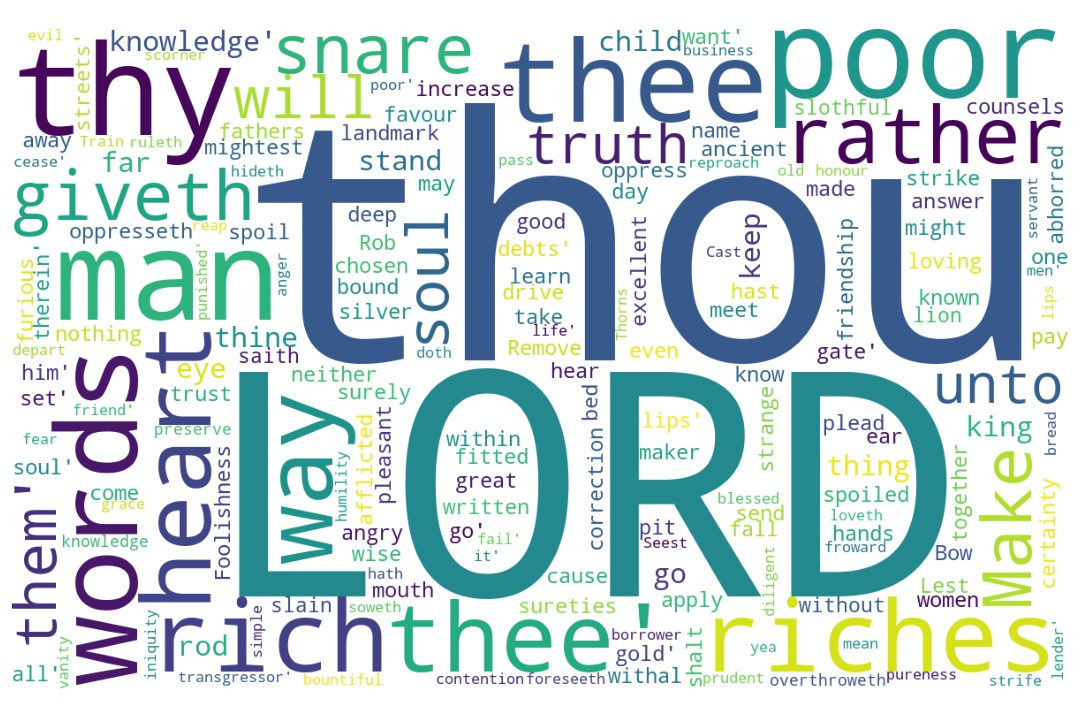
\includegraphics[width=\linewidth]{20OT-Proverbs/Proverb22-WordCloud.jpg}
  \caption{Proverb 22 Word Cloud}
  \label{fig:Proverb 22 word Cloud}
\end{figure}


\marginpar{\scriptsize \centering \fcolorbox{bone}{lime}{\textbf{AN ALL-SEEING GOD}}\\ (Proverb 22:1-29) \begin{compactenum}[I.][8]
    \item \textbf{Are all Around!}(\index[scripture]{Proverbs!Pro 05:21}  \index[scripture]{Proverbs!Pro 15:03}  \index[scripture]{Zechariah!Zch 04:10} (Pro 5:21, Pro 15:3, Zech 4:10)
    \item \textbf{Appraise the Situation} \index[scripture]{1 Kings!1Kng 16:25} \index[scripture]{2 Chronicles!2Chr 14:2}  \index[scripture]{2 Chronicles!2 Chr 21:06}  \index[scripture]{2 Chronicles!2 Chr 29:06} (1Kng 16:25, 2Chr 14:2, 2Chr 21:16, 2Chr 29:6)
    \item \textbf{Are Active} \index[scripture]{Proverbs!Pro 22:12} (Pro 22:12)
    \item \textbf{Approve} \index[scripture]{2 Samuel!2 Sam 15:25} \index[scripture]{Isaiah!Isa 49:05} (2Sam 15:25, Isa 49:5)
    \item \textbf{Are Attentive} (\index[scripture]{Genesis!Gen 6:8}Genesis 06:08, \index[scripture]{2 Chronicles!2 Chr 16:09}2 Chronicles 16:9, \index[scripture]{Psalm!Psa 34:15}Psa 34:15, \index[scripture]{1 Peter!1Pet 03:12}1Pet 3:12)
    \item \textbf{Are Aware} \index[scripture]{Zechariah!Zech 04:10} (Zech 4:10)
    \item \textbf{Analyze} \index[scripture]{Amos!Amo 09:08} (Amos 9:8)
\end{compactenum}}

\marginpar{\scriptsize \centering \fcolorbox{bone}{yellow}{\textbf{SOME ADVICE}}\\ (Proverb 22:1-29) \begin{compactenum}[I.][8]
    \item \textbf{Choice} \index[scripture]{Proverbs!Pro 22:01} (Pro 22:1)
    \item \textbf{Child} \index[scripture]{Proverbs!Pro 22:06}\index[scripture]{Proverbs!Pro 22:15} (Pro 22:6, 15)
    \item \textbf{Contention} \index[scripture]{Proverbs!Pro 22:10} (Pro 22:10)
    \item \textbf{Correction} \index[scripture]{Proverbs!Pro 22:15} (Pro 22:15)
    \item \textbf{Counsels} \index[scripture]{Proverbs!Pro 22:20} (Pro 22:20)
    \item \textbf{Certainty} \index[scripture]{Proverbs!Pro 22:21} (Pro 22:21)
    \item \textbf{Cause} \index[scripture]{Proverbs!Pro 22:23} (Pro 22:23)
\end{compactenum}}

\footnote{\textcolor[cmyk]{0.99998,1,0,0}{\hyperlink{TOC}{Return to end of Table of Contents.}}}\footnote{\href{https://audiobible.com/bible/proverbs_22.html}{\textcolor[cmyk]{0.99998,1,0,0}{Proverbs Audio}}}\textcolor[cmyk]{0.99998,1,0,0}{A \emph{good} name \emph{is} rather to be \fcolorbox{bone}{lime}{chosen} than great riches, \emph{and} loving favour rather than silver and gold.}
[2] \textcolor[cmyk]{0.99998,1,0,0}{The rich and poor meet together: the LORD \emph{is} the maker of them all.}
[3] \textcolor[cmyk]{0.99998,1,0,0}{A prudent \emph{man} foreseeth the evil, and hideth himself: but the simple pass on, and are punished.}
[4] \textcolor[cmyk]{0.99998,1,0,0}{By humility \emph{and} the fear of the LORD \emph{are} riches, and honour, and life.}
[5] \textcolor[cmyk]{0.99998,1,0,0}{Thorns \emph{and} snares \emph{are} in the way of the froward: he that doth keep his soul shall be far from them.}
[6] \textcolor[cmyk]{0.99998,1,0,0}{Train up a \fcolorbox{bone}{lime}{child} in the way he should go: and when he is old, he will not depart from it.}
[7] \textcolor[cmyk]{0.99998,1,0,0}{The rich ruleth over the poor, and the borrower \emph{is} servant to the lender.}
[8] \textcolor[cmyk]{0.99998,1,0,0}{He that soweth iniquity shall reap vanity: and the rod of his anger shall fail.}
[9] \textcolor[cmyk]{0.99998,1,0,0}{He that hath a bountiful eye shall be blessed; for he giveth of his bread to the poor.}\footnote{See Proverbs 21:26 and 14:21. The Roman Vulgate and Alexandrian Septuagint add about eleven to fifteen words not found in the Bible and prove, again, that “Western” and “Alexandrian” manuscripts for the New Testament have the same type of writers, admirers, “preservers,” and believers. For 22:9, the LXX has: ``He that has pity on the poor shall himself be maintained; for he has given of his own bread to the poor. He that gives liberally secures victory an honour; but he takes away the life of them that posses.''}\footnote{\textbf{Proverb 14:21} - He that despiseth his neighbour sinneth: but he that hath mercy on the poor, happy is he.}\footnote{\textbf{Proverb 21:26} - He coveteth greedily all the day long: but the righteous giveth and spareth not.}
[10] \textcolor[cmyk]{0.99998,1,0,0}{Cast out the scorner, and \fcolorbox{bone}{lime}{contention} shall go out; yea, strife and reproach shall cease.}
[11] \textcolor[cmyk]{0.99998,1,0,0}{He that loveth pureness of heart, \emph{for} the grace of his lips the king \emph{shall} \emph{be} his friend.}\footnote{The proverb is clear; especially so in the light of Matthew 5:8 and 2 Samuel 22:27 (see further comment under 21:8). Since God is pure (Hab. 1:13) and the word of God is pure (Psa. 119:140), the “king” (see comments under 20:2, 8 and 21:1) will accept the “pure in heart.” “For the grace of his lips” implies that the pure in heart speaks out of the abundance of his heart (Matt. 5:8). These “lips” are found again in Proverbs 8:6, 10:13, 10:21, 32, 12:19, 14:3, 15:7, and 16:10.}
[12] \textcolor[cmyk]{0.99998,1,0,0}{The eyes of the LORD preserve knowledge, and he overthroweth the words of the transgressor.}
[13] \textcolor[cmyk]{0.99998,1,0,0}{The slothful \emph{man} saith, \emph{There} \emph{is} a lion without, I shall be slain in the streets.}
[14] \textcolor[cmyk]{0.99998,1,0,0}{The mouth of strange women \emph{is} a deep pit: he that is abhorred of the LORD shall fall therein.}
[15] \textcolor[cmyk]{0.99998,1,0,0}{Foolishness \emph{is} bound in the heart of a \fcolorbox{bone}{lime}{child}; \emph{but} the rod of \fcolorbox{bone}{lime}{correction} shall drive it far from him.}
[16] \textcolor[cmyk]{0.99998,1,0,0}{He that oppresseth the poor to increase his \emph{riches,} \emph{and} he that giveth to the rich, \emph{shall} surely \emph{come} to want.}
[17] \textcolor[cmyk]{0.99998,1,0,0}{Bow down thine ear, and hear the words of the wise, and apply thine heart unto my knowledge.}
[18] \textcolor[cmyk]{0.99998,1,0,0}{For \emph{it} \emph{is} a pleasant thing if thou keep them within thee; they shall withal be fitted in thy lips.}
[19] \textcolor[cmyk]{0.99998,1,0,0}{That thy trust may be in the LORD, I have made known to thee this day, even to thee.}
[20] \textcolor[cmyk]{0.99998,1,0,0}{Have not I written to thee excellent things in \fcolorbox{bone}{lime}{counsels} and knowledge,}
[21] \textcolor[cmyk]{0.99998,1,0,0}{That I might make thee know the \fcolorbox{bone}{lime}{certainty} of the words of truth; that thou mightest answer the words of truth to them that send unto thee?}
[22] \textcolor[cmyk]{0.99998,1,0,0}{Rob not the poor, because he \emph{is} poor: neither oppress the afflicted in the gate:}
[23] \textcolor[cmyk]{0.99998,1,0,0}{For the LORD will plead their \fcolorbox{bone}{lime}{cause}, and spoil the soul of those that spoiled them.}
[24] \textcolor[cmyk]{0.99998,1,0,0}{Make no friendship with an angry man; and with a furious man thou shalt not go:}
[25] \textcolor[cmyk]{0.99998,1,0,0}{Lest thou learn his ways, and get a snare to thy soul.}
[26] \textcolor[cmyk]{0.99998,1,0,0}{Be not thou \emph{one} of them that strike hands, \emph{or} of them that are sureties for debts.}
[27] \textcolor[cmyk]{0.99998,1,0,0}{If thou hast nothing to pay, why should he take away thy bed from under thee?}
[28] \textcolor[cmyk]{0.99998,1,0,0}{Remove not the ancient landmark, which thy fathers have set.}\footnote{\textbf{Deuteronomy 19:14} - Thou shalt not remove thy neighbour’s landmark, which they of old time have set in thine inheritance, which thou shalt inherit in the land that the LORD thy God giveth thee to possess it.}\footnote{\textbf{Deuteronomy 27:17} - Cursed be he that removeth his neighbour’s landmark. And all the people shall say, Amen.}\footnote{\textbf{Proverb 23:10} - Remove not the old landmark; and enter not into the fields of the fatherless:}
[29] \textcolor[cmyk]{0.99998,1,0,0}{Seest thou a man diligent in his business? he shall stand before kings; he shall not stand before mean \emph{men}.}\footnote{\textbf{Proverb 21:5} - he thoughts of the diligent tend only to plenteousness; but of every one that is hasty only to want.}\footnote{\textbf{Proverb 27:23} - Be thou diligent to know the state of thy flocks, and look well to thy herds.}\footnote{\textbf{2 Peter 3:14} - Wherefore, beloved, seeing that ye look for such things, be diligent that ye may be found of him in peace, without spot, and blameless.}



\index[NWIV]{19!Proverbs!Pro 22:1}\index[AWIP]{A!Proverbs!Pro 22:1}\index[AWIP]{\emph{good}!Proverbs!Pro 22:1}\index[AWIP]{name!Proverbs!Pro 22:1}\index[AWIP]{\emph{is}!Proverbs!Pro 22:1}\index[AWIP]{rather!Proverbs!Pro 22:1}\index[AWIP]{rather!Proverbs!Pro 22:1 (2)}\index[AWIP]{to!Proverbs!Pro 22:1}\index[AWIP]{be!Proverbs!Pro 22:1}\index[AWIP]{chosen!Proverbs!Pro 22:1}\index[AWIP]{than!Proverbs!Pro 22:1}\index[AWIP]{than!Proverbs!Pro 22:1 (2)}\index[AWIP]{great!Proverbs!Pro 22:1}\index[AWIP]{riches!Proverbs!Pro 22:1}\index[AWIP]{\emph{and}!Proverbs!Pro 22:1}\index[AWIP]{loving!Proverbs!Pro 22:1}\index[AWIP]{favour!Proverbs!Pro 22:1}\index[AWIP]{silver!Proverbs!Pro 22:1}\index[AWIP]{and!Proverbs!Pro 22:1}\index[AWIP]{gold!Proverbs!Pro 22:1}\index[AWIP]{\emph{good}!Proverbs!Pro 22:1}\index[AWIP]{\emph{is}!Proverbs!Pro 22:1}\index[AWIP]{\emph{and}!Proverbs!Pro 22:1}

\index[NWIV]{14!Proverbs!Pro 22:2}\index[AWIP]{The!Proverbs!Pro 22:2}\index[AWIP]{rich!Proverbs!Pro 22:2}\index[AWIP]{and!Proverbs!Pro 22:2}\index[AWIP]{poor!Proverbs!Pro 22:2}\index[AWIP]{meet!Proverbs!Pro 22:2}\index[AWIP]{together!Proverbs!Pro 22:2}\index[AWIP]{the!Proverbs!Pro 22:2}\index[AWIP]{the!Proverbs!Pro 22:2 (2)}\index[AWIP]{LORD!Proverbs!Pro 22:2}\index[AWIP]{\emph{is}!Proverbs!Pro 22:2}\index[AWIP]{maker!Proverbs!Pro 22:2}\index[AWIP]{of!Proverbs!Pro 22:2}\index[AWIP]{them!Proverbs!Pro 22:2}\index[AWIP]{all!Proverbs!Pro 22:2}\index[AWIP]{\emph{is}!Proverbs!Pro 22:2}

\index[NWIV]{17!Proverbs!Pro 22:3}\index[AWIP]{A!Proverbs!Pro 22:3}\index[AWIP]{prudent!Proverbs!Pro 22:3}\index[AWIP]{\emph{man}!Proverbs!Pro 22:3}\index[AWIP]{foreseeth!Proverbs!Pro 22:3}\index[AWIP]{the!Proverbs!Pro 22:3}\index[AWIP]{the!Proverbs!Pro 22:3 (2)}\index[AWIP]{evil!Proverbs!Pro 22:3}\index[AWIP]{and!Proverbs!Pro 22:3}\index[AWIP]{and!Proverbs!Pro 22:3 (2)}\index[AWIP]{hideth!Proverbs!Pro 22:3}\index[AWIP]{himself!Proverbs!Pro 22:3}\index[AWIP]{but!Proverbs!Pro 22:3}\index[AWIP]{simple!Proverbs!Pro 22:3}\index[AWIP]{pass!Proverbs!Pro 22:3}\index[AWIP]{on!Proverbs!Pro 22:3}\index[AWIP]{are!Proverbs!Pro 22:3}\index[AWIP]{punished!Proverbs!Pro 22:3}\index[AWIP]{\emph{man}!Proverbs!Pro 22:3}

\index[NWIV]{14!Proverbs!Pro 22:4}\index[AWIP]{By!Proverbs!Pro 22:4}\index[AWIP]{humility!Proverbs!Pro 22:4}\index[AWIP]{\emph{and}!Proverbs!Pro 22:4}\index[AWIP]{the!Proverbs!Pro 22:4}\index[AWIP]{the!Proverbs!Pro 22:4 (2)}\index[AWIP]{fear!Proverbs!Pro 22:4}\index[AWIP]{of!Proverbs!Pro 22:4}\index[AWIP]{LORD!Proverbs!Pro 22:4}\index[AWIP]{\emph{are}!Proverbs!Pro 22:4}\index[AWIP]{riches!Proverbs!Pro 22:4}\index[AWIP]{and!Proverbs!Pro 22:4}\index[AWIP]{and!Proverbs!Pro 22:4 (2)}\index[AWIP]{honour!Proverbs!Pro 22:4}\index[AWIP]{life!Proverbs!Pro 22:4}\index[AWIP]{\emph{and}!Proverbs!Pro 22:4}\index[AWIP]{\emph{are}!Proverbs!Pro 22:4}

\index[NWIV]{21!Proverbs!Pro 22:5}\index[AWIP]{Thorns!Proverbs!Pro 22:5}\index[AWIP]{\emph{and}!Proverbs!Pro 22:5}\index[AWIP]{snares!Proverbs!Pro 22:5}\index[AWIP]{\emph{are}!Proverbs!Pro 22:5}\index[AWIP]{in!Proverbs!Pro 22:5}\index[AWIP]{the!Proverbs!Pro 22:5}\index[AWIP]{the!Proverbs!Pro 22:5 (2)}\index[AWIP]{way!Proverbs!Pro 22:5}\index[AWIP]{of!Proverbs!Pro 22:5}\index[AWIP]{froward!Proverbs!Pro 22:5}\index[AWIP]{he!Proverbs!Pro 22:5}\index[AWIP]{that!Proverbs!Pro 22:5}\index[AWIP]{doth!Proverbs!Pro 22:5}\index[AWIP]{keep!Proverbs!Pro 22:5}\index[AWIP]{his!Proverbs!Pro 22:5}\index[AWIP]{soul!Proverbs!Pro 22:5}\index[AWIP]{shall!Proverbs!Pro 22:5}\index[AWIP]{be!Proverbs!Pro 22:5}\index[AWIP]{far!Proverbs!Pro 22:5}\index[AWIP]{from!Proverbs!Pro 22:5}\index[AWIP]{them!Proverbs!Pro 22:5}\index[AWIP]{\emph{and}!Proverbs!Pro 22:5}\index[AWIP]{\emph{are}!Proverbs!Pro 22:5}

\index[NWIV]{21!Proverbs!Pro 22:6}\index[AWIP]{Train!Proverbs!Pro 22:6}\index[AWIP]{up!Proverbs!Pro 22:6}\index[AWIP]{a!Proverbs!Pro 22:6}\index[AWIP]{child!Proverbs!Pro 22:6}\index[AWIP]{in!Proverbs!Pro 22:6}\index[AWIP]{the!Proverbs!Pro 22:6}\index[AWIP]{way!Proverbs!Pro 22:6}\index[AWIP]{he!Proverbs!Pro 22:6}\index[AWIP]{he!Proverbs!Pro 22:6 (2)}\index[AWIP]{he!Proverbs!Pro 22:6 (3)}\index[AWIP]{should!Proverbs!Pro 22:6}\index[AWIP]{go!Proverbs!Pro 22:6}\index[AWIP]{and!Proverbs!Pro 22:6}\index[AWIP]{when!Proverbs!Pro 22:6}\index[AWIP]{is!Proverbs!Pro 22:6}\index[AWIP]{old!Proverbs!Pro 22:6}\index[AWIP]{will!Proverbs!Pro 22:6}\index[AWIP]{not!Proverbs!Pro 22:6}\index[AWIP]{depart!Proverbs!Pro 22:6}\index[AWIP]{from!Proverbs!Pro 22:6}\index[AWIP]{it!Proverbs!Pro 22:6}

\index[NWIV]{14!Proverbs!Pro 22:7}\index[AWIP]{The!Proverbs!Pro 22:7}\index[AWIP]{rich!Proverbs!Pro 22:7}\index[AWIP]{ruleth!Proverbs!Pro 22:7}\index[AWIP]{over!Proverbs!Pro 22:7}\index[AWIP]{the!Proverbs!Pro 22:7}\index[AWIP]{the!Proverbs!Pro 22:7 (2)}\index[AWIP]{the!Proverbs!Pro 22:7 (3)}\index[AWIP]{poor!Proverbs!Pro 22:7}\index[AWIP]{and!Proverbs!Pro 22:7}\index[AWIP]{borrower!Proverbs!Pro 22:7}\index[AWIP]{\emph{is}!Proverbs!Pro 22:7}\index[AWIP]{servant!Proverbs!Pro 22:7}\index[AWIP]{to!Proverbs!Pro 22:7}\index[AWIP]{lender!Proverbs!Pro 22:7}\index[AWIP]{\emph{is}!Proverbs!Pro 22:7}

\index[NWIV]{15!Proverbs!Pro 22:8}\index[AWIP]{He!Proverbs!Pro 22:8}\index[AWIP]{that!Proverbs!Pro 22:8}\index[AWIP]{soweth!Proverbs!Pro 22:8}\index[AWIP]{iniquity!Proverbs!Pro 22:8}\index[AWIP]{shall!Proverbs!Pro 22:8}\index[AWIP]{shall!Proverbs!Pro 22:8 (2)}\index[AWIP]{reap!Proverbs!Pro 22:8}\index[AWIP]{vanity!Proverbs!Pro 22:8}\index[AWIP]{and!Proverbs!Pro 22:8}\index[AWIP]{the!Proverbs!Pro 22:8}\index[AWIP]{rod!Proverbs!Pro 22:8}\index[AWIP]{of!Proverbs!Pro 22:8}\index[AWIP]{his!Proverbs!Pro 22:8}\index[AWIP]{anger!Proverbs!Pro 22:8}\index[AWIP]{fail!Proverbs!Pro 22:8}

\index[NWIV]{18!Proverbs!Pro 22:9}\index[AWIP]{He!Proverbs!Pro 22:9}\index[AWIP]{that!Proverbs!Pro 22:9}\index[AWIP]{hath!Proverbs!Pro 22:9}\index[AWIP]{a!Proverbs!Pro 22:9}\index[AWIP]{bountiful!Proverbs!Pro 22:9}\index[AWIP]{eye!Proverbs!Pro 22:9}\index[AWIP]{shall!Proverbs!Pro 22:9}\index[AWIP]{be!Proverbs!Pro 22:9}\index[AWIP]{blessed!Proverbs!Pro 22:9}\index[AWIP]{for!Proverbs!Pro 22:9}\index[AWIP]{he!Proverbs!Pro 22:9}\index[AWIP]{giveth!Proverbs!Pro 22:9}\index[AWIP]{of!Proverbs!Pro 22:9}\index[AWIP]{his!Proverbs!Pro 22:9}\index[AWIP]{bread!Proverbs!Pro 22:9}\index[AWIP]{to!Proverbs!Pro 22:9}\index[AWIP]{the!Proverbs!Pro 22:9}\index[AWIP]{poor!Proverbs!Pro 22:9}

\index[NWIV]{15!Proverbs!Pro 22:10}\index[AWIP]{Cast!Proverbs!Pro 22:10}\index[AWIP]{out!Proverbs!Pro 22:10}\index[AWIP]{out!Proverbs!Pro 22:10 (2)}\index[AWIP]{the!Proverbs!Pro 22:10}\index[AWIP]{scorner!Proverbs!Pro 22:10}\index[AWIP]{and!Proverbs!Pro 22:10}\index[AWIP]{and!Proverbs!Pro 22:10 (2)}\index[AWIP]{contention!Proverbs!Pro 22:10}\index[AWIP]{shall!Proverbs!Pro 22:10}\index[AWIP]{shall!Proverbs!Pro 22:10 (2)}\index[AWIP]{go!Proverbs!Pro 22:10}\index[AWIP]{yea!Proverbs!Pro 22:10}\index[AWIP]{strife!Proverbs!Pro 22:10}\index[AWIP]{reproach!Proverbs!Pro 22:10}\index[AWIP]{cease!Proverbs!Pro 22:10}

\index[NWIV]{18!Proverbs!Pro 22:11}\index[AWIP]{He!Proverbs!Pro 22:11}\index[AWIP]{that!Proverbs!Pro 22:11}\index[AWIP]{loveth!Proverbs!Pro 22:11}\index[AWIP]{pureness!Proverbs!Pro 22:11}\index[AWIP]{of!Proverbs!Pro 22:11}\index[AWIP]{of!Proverbs!Pro 22:11 (2)}\index[AWIP]{heart!Proverbs!Pro 22:11}\index[AWIP]{\emph{for}!Proverbs!Pro 22:11}\index[AWIP]{the!Proverbs!Pro 22:11}\index[AWIP]{the!Proverbs!Pro 22:11 (2)}\index[AWIP]{grace!Proverbs!Pro 22:11}\index[AWIP]{his!Proverbs!Pro 22:11}\index[AWIP]{his!Proverbs!Pro 22:11 (2)}\index[AWIP]{lips!Proverbs!Pro 22:11}\index[AWIP]{king!Proverbs!Pro 22:11}\index[AWIP]{\emph{shall}!Proverbs!Pro 22:11}\index[AWIP]{\emph{be}!Proverbs!Pro 22:11}\index[AWIP]{friend!Proverbs!Pro 22:11}\index[AWIP]{\emph{for}!Proverbs!Pro 22:11}\index[AWIP]{\emph{shall}!Proverbs!Pro 22:11}\index[AWIP]{\emph{be}!Proverbs!Pro 22:11}

\index[NWIV]{15!Proverbs!Pro 22:12}\index[AWIP]{The!Proverbs!Pro 22:12}\index[AWIP]{eyes!Proverbs!Pro 22:12}\index[AWIP]{of!Proverbs!Pro 22:12}\index[AWIP]{of!Proverbs!Pro 22:12 (2)}\index[AWIP]{the!Proverbs!Pro 22:12}\index[AWIP]{the!Proverbs!Pro 22:12 (2)}\index[AWIP]{the!Proverbs!Pro 22:12 (3)}\index[AWIP]{LORD!Proverbs!Pro 22:12}\index[AWIP]{preserve!Proverbs!Pro 22:12}\index[AWIP]{knowledge!Proverbs!Pro 22:12}\index[AWIP]{and!Proverbs!Pro 22:12}\index[AWIP]{he!Proverbs!Pro 22:12}\index[AWIP]{overthroweth!Proverbs!Pro 22:12}\index[AWIP]{words!Proverbs!Pro 22:12}\index[AWIP]{transgressor!Proverbs!Pro 22:12}

\index[NWIV]{16!Proverbs!Pro 22:13}\index[AWIP]{The!Proverbs!Pro 22:13}\index[AWIP]{slothful!Proverbs!Pro 22:13}\index[AWIP]{\emph{man}!Proverbs!Pro 22:13}\index[AWIP]{saith!Proverbs!Pro 22:13}\index[AWIP]{\emph{There}!Proverbs!Pro 22:13}\index[AWIP]{\emph{is}!Proverbs!Pro 22:13}\index[AWIP]{a!Proverbs!Pro 22:13}\index[AWIP]{lion!Proverbs!Pro 22:13}\index[AWIP]{without!Proverbs!Pro 22:13}\index[AWIP]{I!Proverbs!Pro 22:13}\index[AWIP]{shall!Proverbs!Pro 22:13}\index[AWIP]{be!Proverbs!Pro 22:13}\index[AWIP]{slain!Proverbs!Pro 22:13}\index[AWIP]{in!Proverbs!Pro 22:13}\index[AWIP]{the!Proverbs!Pro 22:13}\index[AWIP]{streets!Proverbs!Pro 22:13}\index[AWIP]{\emph{man}!Proverbs!Pro 22:13}\index[AWIP]{\emph{There}!Proverbs!Pro 22:13}\index[AWIP]{\emph{is}!Proverbs!Pro 22:13}

\index[NWIV]{19!Proverbs!Pro 22:14}\index[AWIP]{The!Proverbs!Pro 22:14}\index[AWIP]{mouth!Proverbs!Pro 22:14}\index[AWIP]{of!Proverbs!Pro 22:14}\index[AWIP]{of!Proverbs!Pro 22:14 (2)}\index[AWIP]{strange!Proverbs!Pro 22:14}\index[AWIP]{women!Proverbs!Pro 22:14}\index[AWIP]{\emph{is}!Proverbs!Pro 22:14}\index[AWIP]{a!Proverbs!Pro 22:14}\index[AWIP]{deep!Proverbs!Pro 22:14}\index[AWIP]{pit!Proverbs!Pro 22:14}\index[AWIP]{he!Proverbs!Pro 22:14}\index[AWIP]{that!Proverbs!Pro 22:14}\index[AWIP]{is!Proverbs!Pro 22:14}\index[AWIP]{abhorred!Proverbs!Pro 22:14}\index[AWIP]{the!Proverbs!Pro 22:14}\index[AWIP]{LORD!Proverbs!Pro 22:14}\index[AWIP]{shall!Proverbs!Pro 22:14}\index[AWIP]{fall!Proverbs!Pro 22:14}\index[AWIP]{therein!Proverbs!Pro 22:14}\index[AWIP]{\emph{is}!Proverbs!Pro 22:14}

\index[NWIV]{20!Proverbs!Pro 22:15}\index[AWIP]{Foolishness!Proverbs!Pro 22:15}\index[AWIP]{\emph{is}!Proverbs!Pro 22:15}\index[AWIP]{bound!Proverbs!Pro 22:15}\index[AWIP]{in!Proverbs!Pro 22:15}\index[AWIP]{the!Proverbs!Pro 22:15}\index[AWIP]{the!Proverbs!Pro 22:15 (2)}\index[AWIP]{heart!Proverbs!Pro 22:15}\index[AWIP]{of!Proverbs!Pro 22:15}\index[AWIP]{of!Proverbs!Pro 22:15 (2)}\index[AWIP]{a!Proverbs!Pro 22:15}\index[AWIP]{child!Proverbs!Pro 22:15}\index[AWIP]{\emph{but}!Proverbs!Pro 22:15}\index[AWIP]{rod!Proverbs!Pro 22:15}\index[AWIP]{correction!Proverbs!Pro 22:15}\index[AWIP]{shall!Proverbs!Pro 22:15}\index[AWIP]{drive!Proverbs!Pro 22:15}\index[AWIP]{it!Proverbs!Pro 22:15}\index[AWIP]{far!Proverbs!Pro 22:15}\index[AWIP]{from!Proverbs!Pro 22:15}\index[AWIP]{him!Proverbs!Pro 22:15}\index[AWIP]{\emph{is}!Proverbs!Pro 22:15}\index[AWIP]{\emph{but}!Proverbs!Pro 22:15}

\index[NWIV]{21!Proverbs!Pro 22:16}\index[AWIP]{He!Proverbs!Pro 22:16}\index[AWIP]{that!Proverbs!Pro 22:16}\index[AWIP]{that!Proverbs!Pro 22:16 (2)}\index[AWIP]{oppresseth!Proverbs!Pro 22:16}\index[AWIP]{the!Proverbs!Pro 22:16}\index[AWIP]{the!Proverbs!Pro 22:16 (2)}\index[AWIP]{poor!Proverbs!Pro 22:16}\index[AWIP]{to!Proverbs!Pro 22:16}\index[AWIP]{to!Proverbs!Pro 22:16 (2)}\index[AWIP]{to!Proverbs!Pro 22:16 (3)}\index[AWIP]{increase!Proverbs!Pro 22:16}\index[AWIP]{his!Proverbs!Pro 22:16}\index[AWIP]{\emph{riches}!Proverbs!Pro 22:16}\index[AWIP]{\emph{and}!Proverbs!Pro 22:16}\index[AWIP]{he!Proverbs!Pro 22:16}\index[AWIP]{giveth!Proverbs!Pro 22:16}\index[AWIP]{rich!Proverbs!Pro 22:16}\index[AWIP]{\emph{shall}!Proverbs!Pro 22:16}\index[AWIP]{surely!Proverbs!Pro 22:16}\index[AWIP]{\emph{come}!Proverbs!Pro 22:16}\index[AWIP]{want!Proverbs!Pro 22:16}\index[AWIP]{\emph{riches}!Proverbs!Pro 22:16}\index[AWIP]{\emph{and}!Proverbs!Pro 22:16}\index[AWIP]{\emph{shall}!Proverbs!Pro 22:16}\index[AWIP]{\emph{come}!Proverbs!Pro 22:16}

\index[NWIV]{18!Proverbs!Pro 22:17}\index[AWIP]{Bow!Proverbs!Pro 22:17}\index[AWIP]{down!Proverbs!Pro 22:17}\index[AWIP]{thine!Proverbs!Pro 22:17}\index[AWIP]{thine!Proverbs!Pro 22:17 (2)}\index[AWIP]{ear!Proverbs!Pro 22:17}\index[AWIP]{and!Proverbs!Pro 22:17}\index[AWIP]{and!Proverbs!Pro 22:17 (2)}\index[AWIP]{hear!Proverbs!Pro 22:17}\index[AWIP]{the!Proverbs!Pro 22:17}\index[AWIP]{the!Proverbs!Pro 22:17 (2)}\index[AWIP]{words!Proverbs!Pro 22:17}\index[AWIP]{of!Proverbs!Pro 22:17}\index[AWIP]{wise!Proverbs!Pro 22:17}\index[AWIP]{apply!Proverbs!Pro 22:17}\index[AWIP]{heart!Proverbs!Pro 22:17}\index[AWIP]{unto!Proverbs!Pro 22:17}\index[AWIP]{my!Proverbs!Pro 22:17}\index[AWIP]{knowledge!Proverbs!Pro 22:17}

\index[NWIV]{20!Proverbs!Pro 22:18}\index[AWIP]{For!Proverbs!Pro 22:18}\index[AWIP]{\emph{it}!Proverbs!Pro 22:18}\index[AWIP]{\emph{is}!Proverbs!Pro 22:18}\index[AWIP]{a!Proverbs!Pro 22:18}\index[AWIP]{pleasant!Proverbs!Pro 22:18}\index[AWIP]{thing!Proverbs!Pro 22:18}\index[AWIP]{if!Proverbs!Pro 22:18}\index[AWIP]{thou!Proverbs!Pro 22:18}\index[AWIP]{keep!Proverbs!Pro 22:18}\index[AWIP]{them!Proverbs!Pro 22:18}\index[AWIP]{within!Proverbs!Pro 22:18}\index[AWIP]{thee!Proverbs!Pro 22:18}\index[AWIP]{they!Proverbs!Pro 22:18}\index[AWIP]{shall!Proverbs!Pro 22:18}\index[AWIP]{withal!Proverbs!Pro 22:18}\index[AWIP]{be!Proverbs!Pro 22:18}\index[AWIP]{fitted!Proverbs!Pro 22:18}\index[AWIP]{in!Proverbs!Pro 22:18}\index[AWIP]{thy!Proverbs!Pro 22:18}\index[AWIP]{lips!Proverbs!Pro 22:18}\index[AWIP]{\emph{it}!Proverbs!Pro 22:18}\index[AWIP]{\emph{is}!Proverbs!Pro 22:18}

\index[NWIV]{19!Proverbs!Pro 22:19}\index[AWIP]{That!Proverbs!Pro 22:19}\index[AWIP]{thy!Proverbs!Pro 22:19}\index[AWIP]{trust!Proverbs!Pro 22:19}\index[AWIP]{may!Proverbs!Pro 22:19}\index[AWIP]{be!Proverbs!Pro 22:19}\index[AWIP]{in!Proverbs!Pro 22:19}\index[AWIP]{the!Proverbs!Pro 22:19}\index[AWIP]{LORD!Proverbs!Pro 22:19}\index[AWIP]{I!Proverbs!Pro 22:19}\index[AWIP]{have!Proverbs!Pro 22:19}\index[AWIP]{made!Proverbs!Pro 22:19}\index[AWIP]{known!Proverbs!Pro 22:19}\index[AWIP]{to!Proverbs!Pro 22:19}\index[AWIP]{to!Proverbs!Pro 22:19 (2)}\index[AWIP]{thee!Proverbs!Pro 22:19}\index[AWIP]{thee!Proverbs!Pro 22:19 (2)}\index[AWIP]{this!Proverbs!Pro 22:19}\index[AWIP]{day!Proverbs!Pro 22:19}\index[AWIP]{even!Proverbs!Pro 22:19}

\index[NWIV]{12!Proverbs!Pro 22:20}\index[AWIP]{Have!Proverbs!Pro 22:20}\index[AWIP]{not!Proverbs!Pro 22:20}\index[AWIP]{I!Proverbs!Pro 22:20}\index[AWIP]{written!Proverbs!Pro 22:20}\index[AWIP]{to!Proverbs!Pro 22:20}\index[AWIP]{thee!Proverbs!Pro 22:20}\index[AWIP]{excellent!Proverbs!Pro 22:20}\index[AWIP]{things!Proverbs!Pro 22:20}\index[AWIP]{in!Proverbs!Pro 22:20}\index[AWIP]{counsels!Proverbs!Pro 22:20}\index[AWIP]{and!Proverbs!Pro 22:20}\index[AWIP]{knowledge!Proverbs!Pro 22:20}

\index[NWIV]{27!Proverbs!Pro 22:21}\index[AWIP]{That!Proverbs!Pro 22:21}\index[AWIP]{I!Proverbs!Pro 22:21}\index[AWIP]{might!Proverbs!Pro 22:21}\index[AWIP]{make!Proverbs!Pro 22:21}\index[AWIP]{thee!Proverbs!Pro 22:21}\index[AWIP]{know!Proverbs!Pro 22:21}\index[AWIP]{the!Proverbs!Pro 22:21}\index[AWIP]{the!Proverbs!Pro 22:21 (2)}\index[AWIP]{the!Proverbs!Pro 22:21 (3)}\index[AWIP]{certainty!Proverbs!Pro 22:21}\index[AWIP]{of!Proverbs!Pro 22:21}\index[AWIP]{of!Proverbs!Pro 22:21 (2)}\index[AWIP]{of!Proverbs!Pro 22:21 (3)}\index[AWIP]{words!Proverbs!Pro 22:21}\index[AWIP]{words!Proverbs!Pro 22:21 (2)}\index[AWIP]{truth!Proverbs!Pro 22:21}\index[AWIP]{truth!Proverbs!Pro 22:21 (2)}\index[AWIP]{that!Proverbs!Pro 22:21}\index[AWIP]{that!Proverbs!Pro 22:21 (2)}\index[AWIP]{thou!Proverbs!Pro 22:21}\index[AWIP]{mightest!Proverbs!Pro 22:21}\index[AWIP]{answer!Proverbs!Pro 22:21}\index[AWIP]{to!Proverbs!Pro 22:21}\index[AWIP]{them!Proverbs!Pro 22:21}\index[AWIP]{send!Proverbs!Pro 22:21}\index[AWIP]{unto!Proverbs!Pro 22:21}\index[AWIP]{thee?!Proverbs!Pro 22:21}

\index[NWIV]{15!Proverbs!Pro 22:22}\index[AWIP]{Rob!Proverbs!Pro 22:22}\index[AWIP]{not!Proverbs!Pro 22:22}\index[AWIP]{the!Proverbs!Pro 22:22}\index[AWIP]{the!Proverbs!Pro 22:22 (2)}\index[AWIP]{the!Proverbs!Pro 22:22 (3)}\index[AWIP]{poor!Proverbs!Pro 22:22}\index[AWIP]{poor!Proverbs!Pro 22:22 (2)}\index[AWIP]{because!Proverbs!Pro 22:22}\index[AWIP]{he!Proverbs!Pro 22:22}\index[AWIP]{\emph{is}!Proverbs!Pro 22:22}\index[AWIP]{neither!Proverbs!Pro 22:22}\index[AWIP]{oppress!Proverbs!Pro 22:22}\index[AWIP]{afflicted!Proverbs!Pro 22:22}\index[AWIP]{in!Proverbs!Pro 22:22}\index[AWIP]{gate!Proverbs!Pro 22:22}\index[AWIP]{\emph{is}!Proverbs!Pro 22:22}

\index[NWIV]{16!Proverbs!Pro 22:23}\index[AWIP]{For!Proverbs!Pro 22:23}\index[AWIP]{the!Proverbs!Pro 22:23}\index[AWIP]{the!Proverbs!Pro 22:23 (2)}\index[AWIP]{LORD!Proverbs!Pro 22:23}\index[AWIP]{will!Proverbs!Pro 22:23}\index[AWIP]{plead!Proverbs!Pro 22:23}\index[AWIP]{their!Proverbs!Pro 22:23}\index[AWIP]{cause!Proverbs!Pro 22:23}\index[AWIP]{and!Proverbs!Pro 22:23}\index[AWIP]{spoil!Proverbs!Pro 22:23}\index[AWIP]{soul!Proverbs!Pro 22:23}\index[AWIP]{of!Proverbs!Pro 22:23}\index[AWIP]{those!Proverbs!Pro 22:23}\index[AWIP]{that!Proverbs!Pro 22:23}\index[AWIP]{spoiled!Proverbs!Pro 22:23}\index[AWIP]{them!Proverbs!Pro 22:23}

\index[NWIV]{16!Proverbs!Pro 22:24}\index[AWIP]{Make!Proverbs!Pro 22:24}\index[AWIP]{no!Proverbs!Pro 22:24}\index[AWIP]{friendship!Proverbs!Pro 22:24}\index[AWIP]{with!Proverbs!Pro 22:24}\index[AWIP]{with!Proverbs!Pro 22:24 (2)}\index[AWIP]{an!Proverbs!Pro 22:24}\index[AWIP]{angry!Proverbs!Pro 22:24}\index[AWIP]{man!Proverbs!Pro 22:24}\index[AWIP]{man!Proverbs!Pro 22:24 (2)}\index[AWIP]{and!Proverbs!Pro 22:24}\index[AWIP]{a!Proverbs!Pro 22:24}\index[AWIP]{furious!Proverbs!Pro 22:24}\index[AWIP]{thou!Proverbs!Pro 22:24}\index[AWIP]{shalt!Proverbs!Pro 22:24}\index[AWIP]{not!Proverbs!Pro 22:24}\index[AWIP]{go!Proverbs!Pro 22:24}

\index[NWIV]{12!Proverbs!Pro 22:25}\index[AWIP]{Lest!Proverbs!Pro 22:25}\index[AWIP]{thou!Proverbs!Pro 22:25}\index[AWIP]{learn!Proverbs!Pro 22:25}\index[AWIP]{his!Proverbs!Pro 22:25}\index[AWIP]{ways!Proverbs!Pro 22:25}\index[AWIP]{and!Proverbs!Pro 22:25}\index[AWIP]{get!Proverbs!Pro 22:25}\index[AWIP]{a!Proverbs!Pro 22:25}\index[AWIP]{snare!Proverbs!Pro 22:25}\index[AWIP]{to!Proverbs!Pro 22:25}\index[AWIP]{thy!Proverbs!Pro 22:25}\index[AWIP]{soul!Proverbs!Pro 22:25}

\index[NWIV]{17!Proverbs!Pro 22:26}\index[AWIP]{Be!Proverbs!Pro 22:26}\index[AWIP]{not!Proverbs!Pro 22:26}\index[AWIP]{thou!Proverbs!Pro 22:26}\index[AWIP]{\emph{one}!Proverbs!Pro 22:26}\index[AWIP]{of!Proverbs!Pro 22:26}\index[AWIP]{of!Proverbs!Pro 22:26 (2)}\index[AWIP]{them!Proverbs!Pro 22:26}\index[AWIP]{them!Proverbs!Pro 22:26 (2)}\index[AWIP]{that!Proverbs!Pro 22:26}\index[AWIP]{that!Proverbs!Pro 22:26 (2)}\index[AWIP]{strike!Proverbs!Pro 22:26}\index[AWIP]{hands!Proverbs!Pro 22:26}\index[AWIP]{\emph{or}!Proverbs!Pro 22:26}\index[AWIP]{are!Proverbs!Pro 22:26}\index[AWIP]{sureties!Proverbs!Pro 22:26}\index[AWIP]{for!Proverbs!Pro 22:26}\index[AWIP]{debts!Proverbs!Pro 22:26}\index[AWIP]{\emph{one}!Proverbs!Pro 22:26}\index[AWIP]{\emph{or}!Proverbs!Pro 22:26}

\index[NWIV]{16!Proverbs!Pro 22:27}\index[AWIP]{If!Proverbs!Pro 22:27}\index[AWIP]{thou!Proverbs!Pro 22:27}\index[AWIP]{hast!Proverbs!Pro 22:27}\index[AWIP]{nothing!Proverbs!Pro 22:27}\index[AWIP]{to!Proverbs!Pro 22:27}\index[AWIP]{pay!Proverbs!Pro 22:27}\index[AWIP]{why!Proverbs!Pro 22:27}\index[AWIP]{should!Proverbs!Pro 22:27}\index[AWIP]{he!Proverbs!Pro 22:27}\index[AWIP]{take!Proverbs!Pro 22:27}\index[AWIP]{away!Proverbs!Pro 22:27}\index[AWIP]{thy!Proverbs!Pro 22:27}\index[AWIP]{bed!Proverbs!Pro 22:27}\index[AWIP]{from!Proverbs!Pro 22:27}\index[AWIP]{under!Proverbs!Pro 22:27}\index[AWIP]{thee?!Proverbs!Pro 22:27}

\index[NWIV]{10!Proverbs!Pro 22:28}\index[AWIP]{Remove!Proverbs!Pro 22:28}\index[AWIP]{not!Proverbs!Pro 22:28}\index[AWIP]{the!Proverbs!Pro 22:28}\index[AWIP]{ancient!Proverbs!Pro 22:28}\index[AWIP]{landmark!Proverbs!Pro 22:28}\index[AWIP]{which!Proverbs!Pro 22:28}\index[AWIP]{thy!Proverbs!Pro 22:28}\index[AWIP]{fathers!Proverbs!Pro 22:28}\index[AWIP]{have!Proverbs!Pro 22:28}\index[AWIP]{set!Proverbs!Pro 22:28}

\index[NWIV]{20!Proverbs!Pro 22:29}\index[AWIP]{Seest!Proverbs!Pro 22:29}\index[AWIP]{thou!Proverbs!Pro 22:29}\index[AWIP]{a!Proverbs!Pro 22:29}\index[AWIP]{man!Proverbs!Pro 22:29}\index[AWIP]{diligent!Proverbs!Pro 22:29}\index[AWIP]{in!Proverbs!Pro 22:29}\index[AWIP]{his!Proverbs!Pro 22:29}\index[AWIP]{business?!Proverbs!Pro 22:29}\index[AWIP]{he!Proverbs!Pro 22:29}\index[AWIP]{he!Proverbs!Pro 22:29 (2)}\index[AWIP]{shall!Proverbs!Pro 22:29}\index[AWIP]{shall!Proverbs!Pro 22:29 (2)}\index[AWIP]{stand!Proverbs!Pro 22:29}\index[AWIP]{stand!Proverbs!Pro 22:29 (2)}\index[AWIP]{before!Proverbs!Pro 22:29}\index[AWIP]{before!Proverbs!Pro 22:29 (2)}\index[AWIP]{kings!Proverbs!Pro 22:29}\index[AWIP]{not!Proverbs!Pro 22:29}\index[AWIP]{mean!Proverbs!Pro 22:29}\index[AWIP]{\emph{men}!Proverbs!Pro 22:29}\index[AWIP]{\emph{men}!Proverbs!Pro 22:29}


\section{Proverbs 22 Outlines}

\subsection{My Outlines}

\subsubsection{An All-Seeing God}
%\textbf{Introduction: }
\index[speaker]{Keith Anthony!Proverb 22 (An All-Seeing God)}
\index[series]{Proverbs (Keith Anthony)!Pro 22 (An All-Seeing God)}
\index[date]{2016/05/21!Proverb 22 (An All-Seeing God) (Keith Anthony)}
\textbf{Introduction:} The phrase ``eyes of the Lord'' is found 22 times in scripture, with each  on describing what these ``eyes of the Lord'' are all about. Every wonder if someone was watching? Someone is. These eyes:\begin{compactenum}[I.]
    \item \textbf{Are all Around!} (\index[scripture]{Proverbs!Pro 05:21}Prov 5:21, \index[scripture]{Proverbs!Prov 15:03}Pro 15:3, \index[scripture]{Zechariah!Zch 04:10}Zech  4:10)
    \item \textbf{Appraise the Situation} (\index[scripture]{1 Kings!1 Kng 16:25}1 Kings 16:25, \index[scripture]{2 Chronicles!2 Chr 14:2}2 Chron 14:2, \index[scripture]{2 Chronicles!2 Chr 21:06}2 Chron 21:6, \index[scripture]{2 Chronicles!2 Chr 29:06}2 Chron 29:6)
    \item \textbf{Are Active} (\index[scripture]{Proverbs!Pro 22:12}Pro 22:12)
    \item \textbf{Approve} (\index[scripture]{2 Samuel!2 Sam 15:25}2 Sam 15:25, \index[scripture]{Isaiah!Isa 49:05}Isa 49:5)
    \item \textbf{Are Attentive} (\index[scripture]{Genesis!Gen 6:8}Gen 06:08, \index[scripture]{2 Chronicles!2 Chr 16:09}2 Chron 16:9, \index[scripture]{Psalm!Psa 34:15}Psalm 34:15, \index[scripture]{1 Peter!1 Pet 03:12}1 Pet 3:12)
    \item \textbf{Are Aware} (\index[scripture]{Zechariah!Zch 04:10}Zech 4:10)
    \item \textbf{Analyze} (\index[scripture]{Amos!Amo 09:08}Amos 9:8)
\end{compactenum}


\subsection{Outlines from Others}



\section{Proverb 22 Comments}

\subsection{Numeric Nuggets}
\textbf{500: } Psalm 22 is the 500$^{th}$ chapter in the Bible.\\
\noindent \textbf{13:} Verse 2 has 13 unique words.

\subsection{Proverb 22 Repeated Phrases}


%%%%%%%%%%
%%%%%%%%%%
\normalsize
 
\begin{center}
\begin{longtable}{|p{3.0in}|p{0.5in}|}
\caption[Proverb 22 Repeated Phrases]{Proverb 22 Repeated Phrases}\label{table:Repeated Phrases Proverb 22} \\
\hline \multicolumn{1}{|c|}{\textbf{Phrase}} & \multicolumn{1}{c|}{\textbf{Frequency}} \\ \hline 
\endfirsthead
 
\multicolumn{2}{c}
{{\bfseries \tablename\ \thetable{} -- continued from previous page}} \\  
\hline \multicolumn{1}{|c|}{\textbf{Phrase}} & \multicolumn{1}{c|}{\textbf{Frequency}} \\ \hline 
\endhead
 
\hline \multicolumn{2}{c}{{ }} \\ \hline
\endfoot 
of the & 7\\ \hline 
the LORD & 6\\ \hline 
in the & 6\\ \hline 
the poor & 4\\ \hline 
He that & 4\\ \hline 
the words & 4\\ \hline 
the words of & 4\\ \hline 
words of & 4\\ \hline 
of them & 3\\ \hline 
of the LORD & 3\\ \hline 
he that & 3\\ \hline 
shall be & 3\\ \hline 
to the & 3\\ \hline 
of his & 3\\ \hline 
\emph{is} a & 3\\ \hline 
to thee & 3\\ \hline 
them that & 3\\ \hline 
\end{longtable}
\end{center}



%%%%%%%%%%
%%%%%%%%%%



%\newpage
\section{Proverb 22 Statistics}

%%%%%%%%%%%%%%%%%%%%%%%%%%%
%%%%% Word Statistics
%%%%%%%%%%%%%%%%%%%%%%%%%%

\normalsize
\subsection{Chapter Word Statistics}


%%%%%%%%%%
%%%%%%%%%%
 
\begin{center}
\begin{longtable}{l|c|c|c|c}
\caption[Stats for Proverb 22]{Stats for Proverb 22} \label{table:Stats for Proverb 22} \\ 
\hline \multicolumn{1}{|c|}{\textbf{Verse(s)}} & \multicolumn{1}{|c|}{\textbf{Count}} & \multicolumn{1}{|c|}{\textbf{Unique}} & \multicolumn{1}{|c|}{\textbf{Italics}} & \multicolumn{1}{|c|}{\textbf{Uniq Italic}}  \\ \hline 
\endfirsthead
 
\multicolumn{5}{c}
{{\bfseries \tablename\ \thetable{} -- continued from previous page}} \\  
\hline \multicolumn{1}{|c|}{\textbf{Verse(s)}} & \multicolumn{1}{|c|}{\textbf{Count}} & \multicolumn{1}{|c|}{\textbf{Unique}} & \multicolumn{1}{|c|}{\textbf{Italics}} & \multicolumn{1}{|c|}{\textbf{Uniq Italic}}  \\ \hline 
\endhead
 
\hline \multicolumn{5}{|r|}{{Continued if needed}} \\ \hline
\endfoot 
1 & 19 & 17 & 3 & 3\\ \hline
2 & 14 & 13 & 1 & 1\\ \hline
3 & 17 & 15 & 1 & 1\\ \hline
4 & 14 & 12 & 2 & 2\\ \hline
5 & 21 & 20 & 2 & 2\\ \hline
6 & 21 & 19 & 0 & 0\\ \hline
7 & 14 & 12 & 1 & 1\\ \hline
8 & 15 & 14 & 0 & 0\\ \hline
9 & 18 & 18 & 0 & 0\\ \hline
10 & 15 & 12 & 0 & 0\\ \hline
11 & 18 & 15 & 3 & 3\\ \hline
12 & 15 & 12 & 0 & 0\\ \hline
13 & 16 & 16 & 3 & 3\\ \hline
14 & 19 & 18 & 1 & 1\\ \hline
15 & 20 & 18 & 2 & 2\\ \hline
16 & 21 & 17 & 4 & 4\\ \hline
17 & 18 & 15 & 0 & 0\\ \hline
18 & 20 & 20 & 2 & 2\\ \hline
19 & 19 & 17 & 0 & 0\\ \hline
20 & 12 & 12 & 0 & 0\\ \hline
21 & 27 & 19 & 0 & 0\\ \hline
22 & 15 & 12 & 1 & 1\\ \hline
23 & 16 & 15 & 0 & 0\\ \hline
24 & 16 & 14 & 0 & 0\\ \hline
25 & 12 & 12 & 0 & 0\\ \hline
26 & 17 & 14 & 2 & 2\\ \hline
27 & 16 & 16 & 0 & 0\\ \hline
28 & 10 & 10 & 0 & 0\\ \hline
29 & 20 & 16 & 1 & 1\\ \hline
\hline \hline
Total & 495 & 244 & 29 & 16




\end{longtable}
\end{center}

%%%%%%%%%%
%%%%%%%%%%


\subsection{Words by Frequency}


\begin{center}
\begin{longtable}{l|r}
\caption[Word Frequencies in Proverb 22]{Word Frequencies in Proverb 22} \label{table:WordsIn-Proverb-22} \\ 
\hline \multicolumn{1}{|c|}{\textbf{Word}} & \multicolumn{1}{c|}{\textbf{Frequency}} \\ \hline 
\endfirsthead
  
\multicolumn{2}{c}  
{{\bfseries \tablename\ \thetable{} -- continued from previous page}} \\   
\hline \multicolumn{1}{|c|}{\textbf{Word}} & \multicolumn{1}{c|}{\textbf{Frequency}} \\ \hline   
\endhead  
  
\hline \multicolumn{2}{|r|}{{Continue}} \\ \hline  
\endfoot  
  
\hline \hline  
\endlastfoot  
  
the & 38\\ \hline 
of & 20\\ \hline 
and & 18\\ \hline 
to & 12\\ \hline 
he & 12\\ \hline 
that & 12\\ \hline 
shall & 12\\ \hline 
in & 9\\ \hline 
a & 9\\ \hline 
\emph{is} & 8\\ \hline 
his & 8\\ \hline 
them & 7\\ \hline 
not & 7\\ \hline 
thou & 7\\ \hline 
thee & 7\\ \hline 
be & 6\\ \hline 
poor & 6\\ \hline 
LORD & 6\\ \hline 
The & 5\\ \hline 
thy & 5\\ \hline 
\emph{and} & 4\\ \hline 
from & 4\\ \hline 
He & 4\\ \hline 
words & 4\\ \hline 
I & 4\\ \hline 
rich & 3\\ \hline 
soul & 3\\ \hline 
go & 3\\ \hline 
heart & 3\\ \hline 
knowledge & 3\\ \hline 
man & 3\\ \hline 
A & 2\\ \hline 
rather & 2\\ \hline 
than & 2\\ \hline 
riches & 2\\ \hline 
\emph{man} & 2\\ \hline 
are & 2\\ \hline 
\emph{are} & 2\\ \hline 
way & 2\\ \hline 
keep & 2\\ \hline 
far & 2\\ \hline 
child & 2\\ \hline 
should & 2\\ \hline 
is & 2\\ \hline 
will & 2\\ \hline 
it & 2\\ \hline 
rod & 2\\ \hline 
for & 2\\ \hline 
giveth & 2\\ \hline 
out & 2\\ \hline 
lips & 2\\ \hline 
\emph{shall} & 2\\ \hline 
thine & 2\\ \hline 
unto & 2\\ \hline 
For & 2\\ \hline 
That & 2\\ \hline 
have & 2\\ \hline 
truth & 2\\ \hline 
with & 2\\ \hline 
stand & 2\\ \hline 
before & 2\\ \hline 
\emph{good} & 1\\ \hline 
name & 1\\ \hline 
chosen & 1\\ \hline 
great & 1\\ \hline 
loving & 1\\ \hline 
favour & 1\\ \hline 
silver & 1\\ \hline 
gold & 1\\ \hline 
meet & 1\\ \hline 
together & 1\\ \hline 
maker & 1\\ \hline 
all & 1\\ \hline 
prudent & 1\\ \hline 
foreseeth & 1\\ \hline 
evil & 1\\ \hline 
hideth & 1\\ \hline 
himself & 1\\ \hline 
but & 1\\ \hline 
simple & 1\\ \hline 
pass & 1\\ \hline 
on & 1\\ \hline 
punished & 1\\ \hline 
By & 1\\ \hline 
humility & 1\\ \hline 
fear & 1\\ \hline 
honour & 1\\ \hline 
life & 1\\ \hline 
Thorns & 1\\ \hline 
snares & 1\\ \hline 
froward & 1\\ \hline 
doth & 1\\ \hline 
Train & 1\\ \hline 
up & 1\\ \hline 
when & 1\\ \hline 
old & 1\\ \hline 
depart & 1\\ \hline 
ruleth & 1\\ \hline 
over & 1\\ \hline 
borrower & 1\\ \hline 
servant & 1\\ \hline 
lender & 1\\ \hline 
soweth & 1\\ \hline 
iniquity & 1\\ \hline 
reap & 1\\ \hline 
vanity & 1\\ \hline 
anger & 1\\ \hline 
fail & 1\\ \hline 
hath & 1\\ \hline 
bountiful & 1\\ \hline 
eye & 1\\ \hline 
blessed & 1\\ \hline 
bread & 1\\ \hline 
Cast & 1\\ \hline 
scorner & 1\\ \hline 
contention & 1\\ \hline 
yea & 1\\ \hline 
strife & 1\\ \hline 
reproach & 1\\ \hline 
cease & 1\\ \hline 
loveth & 1\\ \hline 
pureness & 1\\ \hline 
\emph{for} & 1\\ \hline 
grace & 1\\ \hline 
king & 1\\ \hline 
\emph{be} & 1\\ \hline 
friend & 1\\ \hline 
eyes & 1\\ \hline 
preserve & 1\\ \hline 
overthroweth & 1\\ \hline 
transgressor & 1\\ \hline 
slothful & 1\\ \hline 
saith & 1\\ \hline 
\emph{There} & 1\\ \hline 
lion & 1\\ \hline 
without & 1\\ \hline 
slain & 1\\ \hline 
streets & 1\\ \hline 
mouth & 1\\ \hline 
strange & 1\\ \hline 
women & 1\\ \hline 
deep & 1\\ \hline 
pit & 1\\ \hline 
abhorred & 1\\ \hline 
fall & 1\\ \hline 
therein & 1\\ \hline 
Foolishness & 1\\ \hline 
bound & 1\\ \hline 
\emph{but} & 1\\ \hline 
correction & 1\\ \hline 
drive & 1\\ \hline 
him & 1\\ \hline 
oppresseth & 1\\ \hline 
increase & 1\\ \hline 
\emph{riches} & 1\\ \hline 
surely & 1\\ \hline 
\emph{come} & 1\\ \hline 
want & 1\\ \hline 
Bow & 1\\ \hline 
down & 1\\ \hline 
ear & 1\\ \hline 
hear & 1\\ \hline 
wise & 1\\ \hline 
apply & 1\\ \hline 
my & 1\\ \hline 
\emph{it} & 1\\ \hline 
pleasant & 1\\ \hline 
thing & 1\\ \hline 
if & 1\\ \hline 
within & 1\\ \hline 
they & 1\\ \hline 
withal & 1\\ \hline 
fitted & 1\\ \hline 
trust & 1\\ \hline 
may & 1\\ \hline 
made & 1\\ \hline 
known & 1\\ \hline 
this & 1\\ \hline 
day & 1\\ \hline 
even & 1\\ \hline 
Have & 1\\ \hline 
written & 1\\ \hline 
excellent & 1\\ \hline 
things & 1\\ \hline 
counsels & 1\\ \hline 
might & 1\\ \hline 
make & 1\\ \hline 
know & 1\\ \hline 
certainty & 1\\ \hline 
mightest & 1\\ \hline 
answer & 1\\ \hline 
send & 1\\ \hline 
Rob & 1\\ \hline 
because & 1\\ \hline 
neither & 1\\ \hline 
oppress & 1\\ \hline 
afflicted & 1\\ \hline 
gate & 1\\ \hline 
plead & 1\\ \hline 
their & 1\\ \hline 
cause & 1\\ \hline 
spoil & 1\\ \hline 
those & 1\\ \hline 
spoiled & 1\\ \hline 
Make & 1\\ \hline 
no & 1\\ \hline 
friendship & 1\\ \hline 
an & 1\\ \hline 
angry & 1\\ \hline 
furious & 1\\ \hline 
shalt & 1\\ \hline 
Lest & 1\\ \hline 
learn & 1\\ \hline 
ways & 1\\ \hline 
get & 1\\ \hline 
snare & 1\\ \hline 
Be & 1\\ \hline 
\emph{one} & 1\\ \hline 
strike & 1\\ \hline 
hands & 1\\ \hline 
\emph{or} & 1\\ \hline 
sureties & 1\\ \hline 
debts & 1\\ \hline 
If & 1\\ \hline 
hast & 1\\ \hline 
nothing & 1\\ \hline 
pay & 1\\ \hline 
why & 1\\ \hline 
take & 1\\ \hline 
away & 1\\ \hline 
bed & 1\\ \hline 
under & 1\\ \hline 
Remove & 1\\ \hline 
ancient & 1\\ \hline 
landmark & 1\\ \hline 
which & 1\\ \hline 
fathers & 1\\ \hline 
set & 1\\ \hline 
Seest & 1\\ \hline 
diligent & 1\\ \hline 
business & 1\\ \hline 
kings & 1\\ \hline 
mean & 1\\ \hline 
\emph{men} & 1\\ \hline 
\end{longtable}  
\end{center}  


  
\normalsize  

  
  


\subsection{Words Alphabetically}


\begin{center}
\begin{longtable}{l|r}
\caption[Word Frequencies in Proverb 22]{Word Frequencies in Proverb 22} \label{table:WordsIn-Proverb-22} \\ 
\hline \multicolumn{1}{|c|}{\textbf{Word}} & \multicolumn{1}{c|}{\textbf{Frequency}} \\ \hline 
\endfirsthead
  
\multicolumn{2}{c}  
{{\bfseries \tablename\ \thetable{} -- continued from previous page}} \\   
\hline \multicolumn{1}{|c|}{\textbf{Word}} & \multicolumn{1}{c|}{\textbf{Frequency}} \\ \hline   
\endhead  
  
\hline \multicolumn{2}{|r|}{{Continue}} \\ \hline  
\endfoot  
  
\hline \hline  
\endlastfoot  
  
A & 2\\ \hline 
Be & 1\\ \hline 
Bow & 1\\ \hline 
By & 1\\ \hline 
Cast & 1\\ \hline 
Foolishness & 1\\ \hline 
For & 2\\ \hline 
Have & 1\\ \hline 
He & 4\\ \hline 
I & 4\\ \hline 
If & 1\\ \hline 
LORD & 6\\ \hline 
Lest & 1\\ \hline 
Make & 1\\ \hline 
Remove & 1\\ \hline 
Rob & 1\\ \hline 
Seest & 1\\ \hline 
That & 2\\ \hline 
The & 5\\ \hline 
Thorns & 1\\ \hline 
Train & 1\\ \hline 
\emph{There} & 1\\ \hline 
\emph{and} & 4\\ \hline 
\emph{are} & 2\\ \hline 
\emph{be} & 1\\ \hline 
\emph{but} & 1\\ \hline 
\emph{come} & 1\\ \hline 
\emph{for} & 1\\ \hline 
\emph{good} & 1\\ \hline 
\emph{is} & 8\\ \hline 
\emph{it} & 1\\ \hline 
\emph{man} & 2\\ \hline 
\emph{men} & 1\\ \hline 
\emph{one} & 1\\ \hline 
\emph{or} & 1\\ \hline 
\emph{riches} & 1\\ \hline 
\emph{shall} & 2\\ \hline 
a & 9\\ \hline 
abhorred & 1\\ \hline 
afflicted & 1\\ \hline 
all & 1\\ \hline 
an & 1\\ \hline 
ancient & 1\\ \hline 
and & 18\\ \hline 
anger & 1\\ \hline 
angry & 1\\ \hline 
answer & 1\\ \hline 
apply & 1\\ \hline 
are & 2\\ \hline 
away & 1\\ \hline 
be & 6\\ \hline 
because & 1\\ \hline 
bed & 1\\ \hline 
before & 2\\ \hline 
blessed & 1\\ \hline 
borrower & 1\\ \hline 
bound & 1\\ \hline 
bountiful & 1\\ \hline 
bread & 1\\ \hline 
business & 1\\ \hline 
but & 1\\ \hline 
cause & 1\\ \hline 
cease & 1\\ \hline 
certainty & 1\\ \hline 
child & 2\\ \hline 
chosen & 1\\ \hline 
contention & 1\\ \hline 
correction & 1\\ \hline 
counsels & 1\\ \hline 
day & 1\\ \hline 
debts & 1\\ \hline 
deep & 1\\ \hline 
depart & 1\\ \hline 
diligent & 1\\ \hline 
doth & 1\\ \hline 
down & 1\\ \hline 
drive & 1\\ \hline 
ear & 1\\ \hline 
even & 1\\ \hline 
evil & 1\\ \hline 
excellent & 1\\ \hline 
eye & 1\\ \hline 
eyes & 1\\ \hline 
fail & 1\\ \hline 
fall & 1\\ \hline 
far & 2\\ \hline 
fathers & 1\\ \hline 
favour & 1\\ \hline 
fear & 1\\ \hline 
fitted & 1\\ \hline 
for & 2\\ \hline 
foreseeth & 1\\ \hline 
friend & 1\\ \hline 
friendship & 1\\ \hline 
from & 4\\ \hline 
froward & 1\\ \hline 
furious & 1\\ \hline 
gate & 1\\ \hline 
get & 1\\ \hline 
giveth & 2\\ \hline 
go & 3\\ \hline 
gold & 1\\ \hline 
grace & 1\\ \hline 
great & 1\\ \hline 
hands & 1\\ \hline 
hast & 1\\ \hline 
hath & 1\\ \hline 
have & 2\\ \hline 
he & 12\\ \hline 
hear & 1\\ \hline 
heart & 3\\ \hline 
hideth & 1\\ \hline 
him & 1\\ \hline 
himself & 1\\ \hline 
his & 8\\ \hline 
honour & 1\\ \hline 
humility & 1\\ \hline 
if & 1\\ \hline 
in & 9\\ \hline 
increase & 1\\ \hline 
iniquity & 1\\ \hline 
is & 2\\ \hline 
it & 2\\ \hline 
keep & 2\\ \hline 
king & 1\\ \hline 
kings & 1\\ \hline 
know & 1\\ \hline 
knowledge & 3\\ \hline 
known & 1\\ \hline 
landmark & 1\\ \hline 
learn & 1\\ \hline 
lender & 1\\ \hline 
life & 1\\ \hline 
lion & 1\\ \hline 
lips & 2\\ \hline 
loveth & 1\\ \hline 
loving & 1\\ \hline 
made & 1\\ \hline 
make & 1\\ \hline 
maker & 1\\ \hline 
man & 3\\ \hline 
may & 1\\ \hline 
mean & 1\\ \hline 
meet & 1\\ \hline 
might & 1\\ \hline 
mightest & 1\\ \hline 
mouth & 1\\ \hline 
my & 1\\ \hline 
name & 1\\ \hline 
neither & 1\\ \hline 
no & 1\\ \hline 
not & 7\\ \hline 
nothing & 1\\ \hline 
of & 20\\ \hline 
old & 1\\ \hline 
on & 1\\ \hline 
oppress & 1\\ \hline 
oppresseth & 1\\ \hline 
out & 2\\ \hline 
over & 1\\ \hline 
overthroweth & 1\\ \hline 
pass & 1\\ \hline 
pay & 1\\ \hline 
pit & 1\\ \hline 
plead & 1\\ \hline 
pleasant & 1\\ \hline 
poor & 6\\ \hline 
preserve & 1\\ \hline 
prudent & 1\\ \hline 
punished & 1\\ \hline 
pureness & 1\\ \hline 
rather & 2\\ \hline 
reap & 1\\ \hline 
reproach & 1\\ \hline 
rich & 3\\ \hline 
riches & 2\\ \hline 
rod & 2\\ \hline 
ruleth & 1\\ \hline 
saith & 1\\ \hline 
scorner & 1\\ \hline 
send & 1\\ \hline 
servant & 1\\ \hline 
set & 1\\ \hline 
shall & 12\\ \hline 
shalt & 1\\ \hline 
should & 2\\ \hline 
silver & 1\\ \hline 
simple & 1\\ \hline 
slain & 1\\ \hline 
slothful & 1\\ \hline 
snare & 1\\ \hline 
snares & 1\\ \hline 
soul & 3\\ \hline 
soweth & 1\\ \hline 
spoil & 1\\ \hline 
spoiled & 1\\ \hline 
stand & 2\\ \hline 
strange & 1\\ \hline 
streets & 1\\ \hline 
strife & 1\\ \hline 
strike & 1\\ \hline 
surely & 1\\ \hline 
sureties & 1\\ \hline 
take & 1\\ \hline 
than & 2\\ \hline 
that & 12\\ \hline 
the & 38\\ \hline 
thee & 7\\ \hline 
their & 1\\ \hline 
them & 7\\ \hline 
therein & 1\\ \hline 
they & 1\\ \hline 
thine & 2\\ \hline 
thing & 1\\ \hline 
things & 1\\ \hline 
this & 1\\ \hline 
those & 1\\ \hline 
thou & 7\\ \hline 
thy & 5\\ \hline 
to & 12\\ \hline 
together & 1\\ \hline 
transgressor & 1\\ \hline 
trust & 1\\ \hline 
truth & 2\\ \hline 
under & 1\\ \hline 
unto & 2\\ \hline 
up & 1\\ \hline 
vanity & 1\\ \hline 
want & 1\\ \hline 
way & 2\\ \hline 
ways & 1\\ \hline 
when & 1\\ \hline 
which & 1\\ \hline 
why & 1\\ \hline 
will & 2\\ \hline 
wise & 1\\ \hline 
with & 2\\ \hline 
withal & 1\\ \hline 
within & 1\\ \hline 
without & 1\\ \hline 
women & 1\\ \hline 
words & 4\\ \hline 
written & 1\\ \hline 
yea & 1\\ \hline 
\end{longtable}  
\end{center}  


  
\normalsize  

  
  
\subsection{Word Lengths in Chapter} 
\normalsize 
\begin{center} 
\begin{longtable}{l|p{3.75in}} 
\caption[Words by Length in Proverb 22]{Words by Length in Proverb 22} \label{table:WordsIn-Proverb-22} \\ 
\hline \multicolumn{1}{|c|}{\textbf{Length}} & \multicolumn{1}{c|}{\textbf{Words}} \\ \hline 
\endfirsthead 
 
\multicolumn{2}{c} 
{{\bfseries \tablename\ \thetable{} -- continued from previous page}} \\ 
\hline \multicolumn{1}{|c|}{\textbf{Length}} & \multicolumn{1}{c|}{\textbf{Words}} \\ \hline 
\endhead 
 
\hline \multicolumn{2}{|r|}{{Continued}} \\ \hline 
\endfoot 
 
\hline \hline 
\endlastfoot 
1 & A, a, I\\ \hline 
2 & \emph{is}, to, be, of, on, By, in, he, up, go, is, it, He, \emph{be}, my, \emph{it}, if, no, an, Be, \emph{or}, If\\ \hline 
3 & \emph{and}, and, The, the, all, \emph{man}, but, are, \emph{are}, way, his, far, old, not, rod, eye, for, out, yea, \emph{for}, pit, \emph{but}, him, Bow, ear, For, thy, may, day, Rob, man, get, \emph{one}, pay, why, bed, set, \emph{men}\\ \hline 
4 & \emph{good}, name, than, gold, rich, poor, meet, LORD, them, evil, pass, fear, life, that, doth, keep, soul, from, when, will, over, reap, fail, hath, Cast, lips, king, eyes, lion, deep, fall, \emph{come}, want, down, hear, wise, unto, thou, thee, they, That, have, made, this, even, Have, make, know, send, gate, Make, with, Lest, ways, hast, take, away, mean\\ \hline 
5 & great, maker, shall, Train, child, anger, bread, cease, heart, grace, \emph{shall}, words, saith, \emph{There}, slain, mouth, women, bound, drive, thine, apply, thing, trust, known, might, truth, plead, their, cause, spoil, those, angry, shalt, learn, snare, hands, debts, under, which, Seest, stand, kings\\ \hline 
6 & rather, chosen, riches, loving, favour, silver, hideth, simple, honour, Thorns, snares, should, depart, ruleth, lender, soweth, vanity, giveth, strife, loveth, friend, \emph{riches}, surely, within, withal, fitted, things, answer, strike, Remove, before\\ \hline 
7 & prudent, himself, froward, servant, blessed, scorner, without, streets, strange, therein, written, because, neither, oppress, spoiled, furious, nothing, ancient, fathers\\ \hline 
8 & together, punished, humility, borrower, iniquity, reproach, pureness, preserve, slothful, abhorred, increase, pleasant, counsels, mightest, sureties, landmark, diligent, business\\ \hline 
9 & foreseeth, bountiful, knowledge, excellent, certainty, afflicted\\ \hline 
10 & contention, correction, oppresseth, friendship\\ \hline 
11 & Foolishness\\ \hline 
12 & overthroweth, transgressor\\ \hline 
\end{longtable} 
\end{center} 




%%%%%%%%%%
%%%%%%%%%%
 

%\input{20OT-Proverbs/Example-DEVOTIONAL-Psalm3-DEVOTIONAL-BryanChapel}


%%% For Indexes

%\index[DEVOTIONAL]{TGIF1!Os Hillman (Living for a Cause Greater Than Yourself) - Proverb 19:17!2021/12/21}

%\index[DEVOTIONAL]{TGIF1!Os Hillman (Living for a Cause Greater Than Yourself) - Proverb 19:17!2021/12/21}

















%%% colour: cardinal red - \textcolor[cmyk]{0,0.85,0.70,0.23}{text}


%%%% Example marginpar with a compactenum list --- green color text
%\marginpar{\scriptsize \textcolor[rgb]{0.00,0.545,0.269}{$\rightarrow$7 Abominations: 
%\begin{compactenum}
%	\item A proud look,
%	\item a lying tongue,
%	\item hands that shed innocent blood,
%	\item An heart that deviseth wicked imaginations,
%	\item feet that be swift in running to mischief,
%	\item A false witness that speaketh lies, and
%	\item he that soweth discord among brethren.
%\end{compactenum}}}



%\newpage

%\begin{mdframed}[style=MyFrame]
%\begin{center}
%\begin{longtable}{|p{.5in}|p{3.5in}|}

%\caption[Corruption Alert: Proverbs 18:1]{Corruption Alert: Proverbs 18:1} \label{table:CorruptionProv18:1} \\ 

%\hline  
%\multicolumn{1}{|c|}{\textbf{Version}} & 
%\multicolumn{1}{c|}{\textbf{Corruption}}  \\ \hline 
%\endfirsthead
 
%\multicolumn{2}{c}
%{{\bfseries \tablename\ \thetable{} -- continued from previous page}} \\  \hline  
%\multicolumn{1}{|c|}{\textbf{Version}} & 
%\multicolumn{1}{c|}{\textbf{Corruption}}  \\ \hline 
%\endhead
 
%\hline \multicolumn{2}{|r|}{{Continued on next page}} \\ \hline
%\endfoot 
%\textcolor[rgb]{0.00,0.00,1.00}{AV} & \textcolor[rgb]{0.00,0.00,1.00}{Through desire a man, having separated himself, seeketh \emph{and} intermeddleth with all wisdom.} \\ \hline
%
%ASV &  He that separateth himself seeketh his own desire, And  rageth against all sound wisdom. \\ \hline
%
%CEB &  Unfriendly people look out for themselves; they bicker with sensible people.\\ \hline
%
%ESV & Whoever isolates himself seeks his own desire;  he breaks out against all sound judgment. \\ \hline
%
%NASV &  He who separates himself seeks his own desire, He quarrels against all sound wisdom.\\ \hline
%
%MEV & He who separates himself seeks his own desire; he seeks and quarrels against all wisdom.\\ \hline
%
%NIV &  An unfriendly person pursues selfish ends and against all sound judgment starts quarrels. \\ \hline
%
%NKJV &  A man who isolates himself seeks his own desire; He rages against all wise judgment.\\ \hline
%
%RSV &  He who is estranged seeks pretexts  to break out against all sound judgment.\\ \hline

% \multicolumn{2}{p{4.3in}}{{Modern translations, such as the ASV and others, strike out the first part of the verse, concealing the intent of mankind in genewisdom clearly revealed in scripture. How wonderful is the obfuscated RSV text: ``He who is estranged seeks pretexts.'' What does THAT mean?}} \\ %\hline

%\hline

%\end{longtable}
%\end{center}

%\normalsize 
%\end{mdframed}

%\marginpar{\scriptsize \centering \fcolorbox{black}{lime}{\textbf{OUTIDE THE PLACE OF PROMISE}}\\ (Psalm 137:1--9) 
%\begin{compactenum}[I.][8]
%	\item \textbf{Plight \& Distress} \index[scripture]{Psalms!Psa 137:01} (Psalm 137:1)
%	\item The \textbf{Place Desired} \index[scripture]{Psalms!Psa 137:01} (Psalm 137:1)
%	\item \textbf{Pining \& Despiar} \index[scripture]{Psalms!Psa 137:02} (Psalm 137:2)
%	\item \textbf{Provoked \& Degraded}\index[scripture]{Psalms!Psa 137:03} (Psalm 137:3)
%	\item The \textbf{Predicament Described}\index[scripture]{Psalms!Psa 137:04} (Psalm 137:4)
%	\item A \textbf{Preference Decided}\index[scripture]{Psalms!Psa 137:06} (Psalm 137:6)
%	\item A \textbf{Prediction of Destruction}\index[scripture]{Psalms!Psa 137:08} (Psalm 137:8)
%\end{compactenum} }


%\subsection{Outlines from Others}

%\subsubsection{Words on Wisdom}
%\index[speaker]{John Battles!Proverbs 01 (Words on Wisdom)}
%\index[series]{Proverbs (John Battles)!Proverbs 01 (Words on Wisdom)}
%\index[date]{2016/01/20!Proverbs 01 (Words on Wisdom) (John Battles)}
%\textbf{Lineage}: adpated from S. Conway\\
%\textbf{Introduction}: Proverbs distinctly points out things that a fool does:
%\begin{compactenum}[I.][4]
%	\item \textbf{Welcome to Wisdom} \index[scripture]{Proverbs!Pro 01:01-09}(Proverbs 1:1-9)
%	\item \textbf{Warnings of Wisdom} \index[scripture]{Proverbs!Pro 01:10-19}(Proverbs 1:10-19).
%	\item \textbf{Woe of Wisdom} \index[scripture]{Proverbs!Pro 01:24-32}(Proverbs 1:24-32)
%	\item \textbf{Watchcare of Wisdom} \index[scripture]{Proverbs!Pro 01:33}(Proverbs 1:33).
%\end{compactenum}


%%%%% COLOR FOR MARGINPAR OUTLINES
%% 1  LIME - \marginpar{\scriptsize \centering \fcolorbox{black}{lime}{\textbf{TITLE}}\\ (Passage) 
%% 2. YELLOW - \marginpar{\scriptsize \centering \fcolorbox{black}{yellow}{\textbf{TITLE}}\\ (Passage) 
%% 3. Blue BGND, WHITE LETTERS - \marginpar{\scriptsize \centering \fcolorbox{black}{blue}{\textbf{\textcolor[cmyk]{0,0,0,0}{TITLE}}}\\ (Passage) 
%% 4. black BGND, WHITE LETTERS - \marginpar{\scriptsize \centering \fcolorbox{black}{black}{\textbf{\textcolor[cmyk]{0,0,0,0}{TITLE}}}\\ (Passage) 
%% 5. red BGND, WHITE LETTERS - \marginpar{\scriptsize \centering \fcolorbox{black}{red}{\textbf{\textcolor[cmyk]{0,0,0,0}{TITLE}}}\\ (Passage) 

%%%%%% INCLUSION OF GRAPHIC
%\newpage

%\begin{figure}
%\begin{center}
%\includegraphics[scale=0.5, angle=90]{07OT-Judges/References/b201107i1-large}
%\caption[Summary of the 13 Judges]{Summary of the 13 Judges}
%\label{fig:Summary of the 13 Judges}
%\end{center}
%\end{figure}


%%%%%%%%%%%
%%%%%%%%%%%

% SYTEMATIC THEOLOGY (10 + 2)
% Theology proper – The study of the character of God
% Angelology – The study of angels
% Biblical theology – The study of the Bible
% Christology – The study of Christ
% Ecclesiology – The study of the church
% Eschatology – The study of the end times[5]
% Hamartiology – The study of sin
% Pneumatology – The study of the Holy Spirit
% Soteriology – The study of salvation
% Theological anthropology – The study of the nature of humanity.
% ++
% Moral theology
% Bilical cosomolgy

%%%%%%%%%%%%%%
%%%%%%%%%%%%%%

% \footnote{\href{https://audiobible.com/bible/psalms_91.html}{\textcolor[cmyk]{0.99998,1,0,0}{Psalm 91 Audio}}}

% \marginpar{\scriptsize \centering \fcolorbox{black}{lime}{\textbf{JERUSALEM}}\\
% \fcolorbox{black}{lime}{\textbf{DON'T GO BACK TO EGYPT}} \\ (Isaiah 31:1--9) 

%%%%%%%%%%%%%%
%%% Extra Colors
%%% from https://latexcolor.blogspot.com/2019/10/list-of-latex-colors.html
%%%%%%%%%%%%%%
% \definecolor{champagne}{rgb}{0.97,0.91,0.81}
% \definecolor{bone}{rgb}{0.89,0.85,0.79}
%\titleJE
%

%%%%% EXAMPLE Index entry:
% \index[DOCTRINES]{Eschatology - Millennium!Psalms!Psa 069:036}

%%% for things found 13 times
%\fcolorbox{black}{bone}{TEXT}
\scriptsize

%%%%%%%%%%%%%%%%%%%%%%%%%%%%%
%Indices

\chapter{Indexes}
\printindex[DOCTRINES]
\printindex[scripture]
\printindex[speaker]
%\printindex[series]

\printindex[FACEBOOK]
\printindex[LOCATION]
\printindex[DEVOTIONAL]
\printindex[AWIP]

\printbibliography
\end{document}

